\documentclass[12pt]{book}
\usepackage[pdfa]{hyperref}
\usepackage{standalone}
\usepackage{apacite}
\usepackage{etoolbox}% for the \patchcmd
\makeatletter
% Patch after apacite got loaded!
\patchcmd{\nocite}{\@onlypreamble\document}{\documentclass\sa@documentclass}{}{}
\makeatother
\usepackage{graphicx}
\usepackage{subcaption}
\graphicspath{{/Users/huawei/Desktop/images/}} 
\usepackage{setspace}
\usepackage{booktabs}
\usepackage{tabularx}
\usepackage{xcolor}
\usepackage{amsmath}
\usepackage{pdflscape}
\usepackage[margin=3cm]{geometry}
\usepackage{multirow}
\usepackage{times}
\usepackage{fancyhdr}
\usepackage{color}
\usepackage{dcolumn}
\usepackage{siunitx}
\usepackage{array}
\usepackage{longtable}
\usepackage{tikz}
\usepackage{multicol}
\usepackage{tikzsymbols}
\usepackage{bm}
\usepackage{subcaption}
\usepackage{listings}
\usepackage{array}
\usepackage{siunitx}
\usepackage{titlesec}
\usepackage{regexpatch}
\usepackage[a-1a]{pdfx}
\captionsetup[table]{format=plain, labelsep=newline, justification=RaggedRight, labelfont=bf, textfont=it,  singlelinecheck=off}

\makeatletter
\xpatchcmd{\@@cite}{\def\BCA##1##2{{\@BAstyle ##1}}}{\def\BCA##1##2{{\@BAstyle ##2}}}{}{}
\makeatother

\lstset{language=R,
	basicstyle=\small\ttfamily,
	stringstyle=\color{black},
	%otherkeywords={0,1,2,3,4,5,6,7,8,9},
	morekeywords={TRUE,FALSE, glmer, lmer},
	deletekeywords={data,frame,length,as,character},
	keywordstyle=\color{black}\bfseries,
	commentstyle=\color{black},
}


\hypersetup{
	colorlinks=false, % make the links colored
	linkcolor=black, % color TOC links in blue
	urlcolor=black, % color URLs in red
	linktoc=black, % 'all' will create links for everything in the TOC
	citecolor = none
}
\titleformat*{\subparagraph}{\itshape}

\usetikzlibrary{shapes.geometric, arrows}
\tikzstyle{startstop} = [rectangle, minimum width=1.5cm, minimum height=1cm,text centered, draw=black]
\tikzstyle{process} = [rectangle, rounded corners, minimum width=0.5cm, minimum height=1cm, text width =2.5cm, text centered, draw=black]
\tikzstyle{arrow} = [thick,->,>=stealth]
\usepackage{titlesec}    
\titleformat{\chapter}[display]
{\normalfont%
	\huge% %change this size to your needs for the first line
	\bfseries}{\chaptertitlename\ \thechapter}{20pt}{%
	\LARGE %change this size to your needs for the second line
}
\titlespacing{\chapter}{0pt}{-15pt}{25.5pt}
\titlespacing{name=\chapter}{0pt}{16pt}{15pt}
\raggedbottom

\renewcommand\baselinestretch{1.5}

\newcolumntype{d}[1]{D{.}{.}{#1}}
\def\sym#1{\ifmmode^{#1}\else\(^{#1}\)\fi}

\title{Inglorious Measures: \\ A Linear Mixed-Effects Models approach for modeling implicit measure data within a Rasch framework}
\author{Ottavia M. Epifania}


\begin{document}
	
	
	\frontmatter
	
	%\vspace*{3mm}
	\thispagestyle{empty}
	
	\begin{center}
		
\includegraphics[width=0.25\linewidth]{unipd.png}
	\end{center}
	
	\begin{center}
		\begin{Large}
			\textbf{University of Padova}
			
			Department of Philosophy, Sociology, Education, and Applied Psychology (FISPPA)
		\end{Large}
		
	\end{center}
	
	\vspace{3mm}
	\begin{center}
		\begin{large}
			Ph.D. Course in Psychological Sciences (XXXIII Cycle)
		\end{large}
		
		\begin{huge}
			\bfseries
			Inglorious Measures: \\ A Linear Mixed-Effects Model approach for a Rasch analysis of implicit measure accuracy and time responses
		\end{huge}
		
		
	\end{center}
	
	\vspace{2cm}
	\begin{multicols}{2}
		\begin{flushleft}
%			\begin{large}
				\textbf{Advisor:} Prof. Egidio Robusto
				
				\textbf{Co-Advisor:} Prof. Gianmarco Altoè
	%		\end{large}
			
		\end{flushleft}
		\columnbreak
		\begin{flushright}
			\vspace{1.5cm}
			
				\textbf{Ph.D. Candidate:} Ottavia M. Epifania 
			
		\end{flushright}
		
	\end{multicols}

\vspace{2cm}
	
	\begin{center}
		Academic Year: 2019/2020
	\end{center}
	
	
\newpage 

\ 
\thispagestyle{empty}

\newpage
	
	
	\vspace*{5cm}
	\thispagestyle{empty}
	
	\begin{multicols}{2}
		\vspace*{\textheight}
		\columnbreak
		\begin{flushright}
			\slshape \onehalfspacing
			Muchos años después, frente al pelotón de fusilamiento, el coronel Aureliano Buendía había de recordar aquella tarde remota en que su padre lo llevó a conocer el hielo.
			\\ \vspace{2cm} A Francesco Epifania, \\ che ha trovato il modo di scampare alla lettura di questa Tesi. \\
		\end{flushright}
		
	\end{multicols}
	

	
	\tableofcontents
	

%	\thispagestyle{empty}
	
	\chapter{Preface} \label{chap:preface}
	The advent of measures able to infer mental processes from  speed-categorization tasks opened to the assessment of processes that lie beyond people's awareness, but that can still influence their attitudes and social behaviors. 
	These measures are known as implicit measures, and their use became vastly popular in social sciences.
	Despite the popularity implicit measures gained throughout the past decades, a lot of work still needs to be done to find a psychometrically sound approach to their modeling.
	
	Usually, implicit measures are scored by averaging the response times across stimuli to obtain respondent-specific scores. 
	This approach is extremely easy and provides a clear and interpretable measure of the implicit construct under investigation.  
	However, it overlooks the dependencies related to the systematic variability at both the respondent and stimulus levels, compromising the reliability and replicability of the results  \cite{judd2012}. 
	Given the replicability crisis that has been hitting social psychology from the past few years, the need for more sound, accurate, and reliable methods for the analyses of implicit measure data is of the uttermost importance. 
	The main objective of the thesis is to provide such rigorous methods  by following three paths: (i) the \emph{sound path} for a psychometrically more sound approach to implicit measure data, (ii) the \emph{fair path} for a fairer comparison between implicit measures, and (iii) the \emph{easy path} for an easier, more rigorous, and open source way to score implicit measures.
	
	The sound path constitutes the core of the thesis. It is an attempt at finding new approaches for the analysis of implicit measure data by combining a classic of psychometric theories, the Rasch model, with a Linear Mixed-Effects Model (LMM) approach. The focus is mostly on one of the most popular, used, and studied implicit measure, the Implicit Association Test \cite<IAT;>{Greenwald1998} and on its single category variant, the Single Category IAT \cite<SC-IAT;>{karpinski2006}. Given their structures, the IAT always results in a comparative measure of the preference for one object in comparison to its opposite, while the SC-IAT provides an absolute measure of how much an object is liked. As such, the SC-IAT is often used as an alternative to the IAT when the focus is on the absolute positive or negative evaluation of one object or when a ``natural'' contrast category for the object of interest is not available. 
%	By dropping one of the target category
%	Given its structure, the IAT always results in a relative measure of the preference towards one target object contrasted to its (alleged) opposite. 
%However, there are cases in which the object under investigation does not have a ``natural'' category against which it can be contrasted to or where the focus is on the absolute . 
%In these occurrences, the SC-IAT  is used as an alternative to the IAT for obtaining the measure of interest. 

	Traditionally, Item Response Theory and Rasch modeling treat items (stimuli) as fixed factors (i.e., unknown constants that do not vary as a function of the observational units), while respondents are treated as random factors (i.e., effects that vary according to the observational units, drawn from a larger distribution) \cite{DeBoeck2011}.
	In this work, a slightly different approach is followed, consistent with the data structure of implicit measures. 
	The fully-crossed design characterizing the IAT (see Section \ref{sec:cross}) allows for conceptualizing the stimuli as a manifestation of the super-ordered category they represent. Thus, the specific set of stimuli used in an IAT can be taken as just one the possible sets drawn from the population of stimuli.  The sampling variability of the stimuli should be acknowledged by considering them as random factors and by treating them as random effects to make inferences on the larger population to which they belong. 
	Besides being a statistically more sound approach,
	the acknowledgment of the sampling variability of the stimuli implies that each stimulus potentially has a different functioning and, consequently, a different impact on the observed responses.
	By treating the stimuli as random factors, their sampling variability is accounted for and it can be used to gather the information conveyed by each of them and to investigate their impact on the observed responses \cite{wols2017}. 
    LMMs allow for considering both the respondents and the stimuli as random factors and for treating both of them as random effects at the same time, leading to more detailed and generalizable information at both levels. Moreover, the flexibility of LMMs makes possible to model together data derived from different implicit measures administered at the same time, hence accounting for the between--measures variability typical of \emph{within-subjects} experimental designs.

	However, the use of LMMs for the conjoint analysis of multiple implicit measures administered at the same time is not a common approach. 
	Effect size measures, the so-called \emph{D} scores, are the most popular scoring procedures for the IAT and the SC-IAT, and they are often employed for comparing the  performance of these measures on several variables used as criteria (e.g., the prediction of behavioral outcomes). 
	Beyond being affected by the systematic variability at the stimulus and respondent levels, these scoring procedures present other differences potentially affecting the comparison between the two implicit measures and leading to puzzling results. 
The fair path aims at a fairer comparison between the IAT and the SC-IAT by introducing new scoring algorithms for the IAT and the SC-IAT that minimize the (non-necessary) scoring differences potentially affecting the comparison between the two measures.
The alignment of the IAT and the SC-IAT scoring methods should provide a means for a fairer comparison between the IAT and  the SC-IAT, producing (potentially) more reliable results on the performance of the two measures on different criteria. 
	
Finally, the easy path is oriented at providing open source and easy-to-use tools for the computation of the IAT and SC-IAT scores. By automating the computational procedure and providing it open source, computational mistakes are prevented and the algorithms always result in the same scores that can be easily replicated. %In the long term, this is expected to have beneficial effects on the replicability of the results obtained with implicit measures. 

Taken together, the three paths can enhance the replicability of the results obtained with implicit measures by either introducing psychometrically more valid approaches or by improving the existing ones. The structure of the thesis is as follows.

	In Chapter \ref{chap:intro}, brief definitions of automatic and controlled processes are provided. The main theoretical frameworks that have been proposed for conceptualizing the distinction between the two processes are outlined.  
	The description of the IAT follows, along with the results of a literature review where the use of the IAT in different fields of application was investigated. 
	The SC-IAT is described as well.  
	The chapter ends with a description of the fully-crossed design characterizing implicit measures, and with the reasons why this structure might undermine the replicability of the results if it is not correctly accounted for. 
	
	Both the fair and easy paths are presented in Chapter \ref{chap:classicscore}.  
	The typical and modified scoring procedures of the IAT and the SC-IAT are illustrated.
	The alignment between the administration and scoring procedures of the IAT and the SC-IAT should provide a comparison between the predictive abilities of the two measures  centered on the implicit measures themselves and not on the differences ascribable to the scoring and/or administration procedures.
	The results of an empirical study reported in this chapter highlighted a better performance of the IAT than the SC-IAT in predicting behavioral outcomes. 
% An empirical study aimed at comparing the predictive abilities of the typical and modified scoring procedures is reported. The measure obtained from the IAT always outperformed that obtained from the SC-IAT, regardless of the algorithms.  

	The easy path in Chapter \ref{chap:classicscore} presents two open source alternatives for the computation of the IAT and the SC-IAT typical scoring procedures. 
	One is a Shiny app  \cite<i.e., DscoreApp;>{dscoreapp, shinyfront} for the computation of the IAT \emph{D} score, while the other is an \verb*|R| package for the computation of the IAT and SC-IAT \emph{D} scores \cite<the \texttt{implicitMeasures} package; >{implicitMeasures}. 
	DscoreApp provides the researchers using the IAT with an open source tools able to make the \emph{D} score computation easy, without requiring for any programming experience.
%	Additionally, the replicability of the results is undermined by the many steps that are required for cleaning and preparing the data \cite{ellithorpe2015}.
	% Despite the actual computation of the \emph{D} score is not complicated \emph{per se}, many steps are required for cleaning and preparing the data. 
	%The overall procedure for computing the \emph{D} score is a long and error-prone procedure, which can easily raise issues related to the reproducibibility of the results \cite{ellithorpe2015}. 
	By automating the procedure and providing clear labels and descriptions for the identification of each scoring algorithm, the computational mistakes due to the long and error-prone procedure for cleaning and preparing the data are prevented, and researchers can always be aware of the specific algorithm they use for scoring their data. Taken together, these features might enhance the replicability of the results.
	DscoreApp presents two main shortcomings nonetheless. 
	Firstly, since the code is put into the Shiny interface, it is not possible to call and run it from the command line, hence making impossible to reproduce it. 
	While this might not constitute a problem for the average user, it is a critical issue in an open science framework, according to which all the codes used for the analyses should be accessible at any time.
	Nevertheless, this issue can be overcome by storing the code in a public repository, such as GitHub, as it was done for DscoreApp.
 Secondly, DscoreApp only computes the score for the IAT. 
		The \verb*|implicitMeasures| package is an \verb*|R| package developed for overcoming the two main limitations of DscoreApp. The package also includes functions for cleaning the data sets of the IAT and SC-IAT and for plotting their results at either the individual  or sample level.
	
	Chapter \ref{chap:formalModel} provides an overview of the main modeling frameworks that have been introduced for modeling IAT data. 
	These frameworks can be distinguished according to the type of responses used for the estimation of the parameters. 
	The Quad model \cite{Conrey2005} and the ReAL model \cite{Meissner2013} are based on accuracy responses, while the Diffusion model \cite{Klauer2007} and the Discrimination-Association model \cite{stefanutti2013} account for both the accuracy and time responses. 
	Regardless of the type of responses they consider, these models are able to disentangle the most automatic processes from the most controlled ones intervening during the performance at the IAT. 
	A common finding of these models is that the automatic associations are just one of the possible processes captured by the IAT. Other controlled processes, such as the recoding of the stimuli (ReAL, Diffusion Model) or the suppression of the automatically activated responses (Quad model), play an important role as well. 
	Despite their usefulness for the disentanglement of the cognitive processes underlying the IAT effect, none of these models  provides a detailed information at the level of the individual stimulus. 
	Given the importance of the stimuli selection for a correct functioning of the IAT \cite<e.g.,>{bluemke2006}, the need for models able to provide detailed information at the stimulus level is crucial.  
 Moreover, all these models neglect the variability due to the fully-crossed structure of the IAT data. 
	A Rasch modeling of the IAT data provides fine-grained information on the functioning of the stimuli, allowing for the identification of the stimuli that give the highest contribution to the IAT effect. This information can be used for delving deeper on the automatic associations driving the IAT effect, and hence to obtain a better understanding of the measure itself. 
	However, the applications of the Rasch model to the IAT data are not save from criticisms. The most outstanding one is related to the discretization of the time responses needed for the application of this model, which might cause a large loss of information.
	Moreover, also this approach does not account for the variability in the IAT data. 
	
	An introduction to the Rasch and log-normal models is provided in the first section of Chapter \ref{chap:modelsIAT}. 
	The limitations of the application of the Rasch model to complex data structures such as that of the IAT and its similarities with the structure of Generalized Linear (Mixed-Effects) Models are illustrated. 
	Given that the Rasch model is equivalent to a Generalized Linear Model (GLM) with a \emph{logit} link function (i.e., the natural link function for binomial accuracy responses), the model matrix of the GLM can be extended to include the random effects able to address the sampling variability of the random factors in the IAT data. As such, the Rasch model estimates from IAT data can be obtained by employing Generalized Linear Mixed-Effects Models (GLMMs). 
	The use of GLMMs for estimating the Rasch model parameters accounts for the variability generating local dependence at the trial level, hence resulting in more reliable estimates. 
 By considering the normal density distribution of the log-time responses, the log-normal model allows for obtaining a parametrization of the data analogous to that provided by the Rasch model, while avoiding the discretization of the time responses needed for the application of the Rasch Model. 
	The estimates of the log-normal model parameters can be obtained by applying Linear Mixed-Effects Models (LMMs) to the log-transformed time responses of the IAT.
	The estimates of the Rasch and log-normal models do not directly result from the application of the (G)LMMs to the accuracy or log-time responses, but are obtained by adding the marginal modes of each level of the random effects (\emph{Best Linear Unbiased Predictors}, BLUP) to the estimates of the fixed effects. The specification of  models with different random structures allows for obtaining information at different levels of granularity on either the respondents or the stimuli.
	
	The second section of Chapter \ref{chap:modelsIAT} presents the specification of models with different random structures for a meaningful Rasch and log-normal analysis of the IAT data. 
	Three models for accuracy responses and three models for log-time responses are specified for obtaining the estimates of the Rasch and log-normal models, respectively. 
	Besides the assumption on the distribution of the error term, the random structures of the accuracy and log-time models are identical. 
	The error term for the accuracy responses is modeled by assuming a logistic distribution, while the one for the log-time responses is supposed to follow a normal distribution. 
	The random structures of the models are ordered according to their complexity, with the first one being the simplest one (i.e., Null model). 
	The second and third models have the same degree of complexity. They differ from each other according to the random factor on which they allow for the multidimensionality of the error variance, either the stimuli or the respondents. 
	
	Two empirical applications of the models presented in the second section of Chapter \ref{chap:modelsIAT} are illustrated in Chapter \ref{chap:IATempirical}.
	The first application was aimed at investigating the validity of the proposed models for the analysis of the IAT data. To pursue this aim, a Race IAT was employed and the relationship between the estimates obtained from the Rasch and log-normal models and the typical IAT scoring was investigated. By obtaining condition--specific stimulus estimates of the Rasch model, it was possible to investigate the contribution given by each stimulus to the IAT effect, resulting in a better understanding of the measure itself and in the identification of  malfunctioning stimuli that should be replaced or removed. The condition--specific respondent estimates of the log-normal model, combined with the overall respondent estimates of the Rasch model, brought further evidence in favor of the speed-accuracy trade-off and allowed for a better understanding of the IAT measure as expressed by the typical scoring algorithm. 
	
	The second application was aimed at understanding whether the estimates provided by the proposed modeling framework do result in a better inference of the implicit construct under investigation. As such, the model estimates are expected to lead to a better prediction of behavioral outcomes than the typical scoring procedure of the IAT. 
	The second application was also aimed at testing the usefulness of the condition--specific stimulus estimates. If the stimulus estimates truly allow for pinpointing the most informative stimuli, as well as the least informative ones, a higher amount of information should be obtained by selecting only the former ones to create smaller but highly informative data sets. The \emph{D} score computed on the reduced data set should be more reliable than the one computed on the entire data set, and  potentially results in a better prediction of behavioral outcomes.  
	An IAT for the implicit assessment of the preference for dark or milk chocolate (Chocolate IAT) was employed for pursuing these aims. 
	The Rasch and log-normal model estimates resulted in a better measure of the implicit preference, which in turn led to a better prediction of the behavioral outcome than the one provided by the typical scoring procedure. 
	Moreover, the information on the contribution of each stimulus to the IAT effect allowed  for reducing the across-trial variability by creating smaller data sets with only the most informative stimuli. 
	The \emph{D} scores computed on the reduced data set resulted in a better prediction than those computed on the entire data set, further highlighting the sensitivity of the typical scoring measures to the across-trial variability in the IAT data. 

Despite the approach presented in Chapter \ref{chap:classicscore} provides a fairer comparison between the predictive abilities of the IAT and the SC-IAT, the \emph{post-hoc} separation of measures originally administered together represents its main fallacy. 
	When multiple measures are administered concurrently in a \emph{within-subjects} experimental design, each of them comes with its peculiar data structure and related variability. 
	Additionally, other sources of variability have to be expected, such as the within--respondents between--measures variability and the within--stimuli between--measures variability, if the same sample of stimuli is used across measures.
	Therefore, sources of variability other the ones within each measure should be taken into account to obtain reliable estimates.  
	Chapter \ref{chap:comprehensiveModels} presents a comprehensive modeling approach for multiple implicit measures administered together. 
	The chapter firstly introduces the use of the models presented in Chapter \ref{chap:modelsIAT} for the separate modeling of the IAT and the SC-IAT. This was done for mainly two reasons. Firstly, to investigate the soundness of the proposed approach for modeling measures other than the IAT. Secondly, to investigate whether and how the model estimates change when the within--respondents between--measures variability and the within--stimuli between--measures variability are not accounted for. 
	Despite this approach overlooks the within--respondents between--measures variability, it should result in more reliable estimates than the \emph{D} score.
	However, the estimates from the application of distinct models are not directly comparable between each other. Consequently, the performances of the respondents between implicit measures cannot be compared, and the stimulus estimates might include uncontrolled variance leading to meaningless (and potentially puzzling) results. 
	The extension of the models to account for other sources of variability, hence allowing for the inclusion of multiple implicit measures in the same model, is illustrated. 
	In these models, the focus is on the respondents, hence the multidimensionality of the error variance is allowed only at the respondent level. 
	
Chapter \ref{chap:comprehensiveApplications} presents an empirical application of the modeling approach presented in Chapter \ref{chap:comprehensiveModels}. Data are the same as those in Chapter \ref{chap:classicscore}, hence including one IAT and two SC-IATs. The predictive abilities of the  model estimates and the typical scoring of each measure were compared.
Both the single measure modeling and the comprehensive approach resulted in condition--specific respondent estimates, although the estimates obtained with the former approach are not directly comparable. 
Furthermore, just by accounting for the method specific variance of each implicit measure is possible to obtain more reliable estimates than the \emph{D} score, as it can be inferred from their better prediction of the behavioral outcome. 
By analyzing the data from each implicit measure separately, it is not possible to rule out whether the different functioning of the stimuli between measures is ascribable to an actual different functioning or to uncontrolled error variance. 
The comprehensive modeling allows for directly comparing the estimates at both the respondent and stimulus levels. Consequently, a better understating of the functioning of each implicit measure is obtained, and more meaningful inferences can be made.  
	Besides resulting in a better prediction of the behavioral outcome than the typical \emph{D} scores, the estimates obtained from the single modeling of implicit measures and from their comprehensive modeling allowed for highlighting the contribution of one of the SC-IATs to the prediction of the behavior. The contribution of the SC-IAT to the prediction of the behavior was completely lost when the typical scoring methods were used. 
	
	
	Finally, Chapter \ref{chap:conclusions} summarizes the findings of the studies reported throughout the thesis, and draws general conclusions based on the evidence reported in all studies. The limitations of the studies are addressed and possible future directions are outlined. 


	\mainmatter
	\thispagestyle{empty}

\newpage

\chapter[Psychological implicit assessment]{Psychological implicit assessment} \label{chap:intro}

In this introductory chapter, a brief definition of automatic and controlled processes is provided, along with a summary of the main theoretical frameworks concerning the distinction of these processes. 

The Implicit Association Test \cite<IAT;>{Greenwald1998} and an overview of its use from the year of its first introduction (1998) to current days are then presented. The main fields of application of the IAT are illustrated as well. 
The issues related to the comparative measure that is gathered from the IAT is addressed by presenting an implicit measure able to provide an absolute evaluation towards one target object, namely the Single Category Implicit Association Test \cite<SC-IAT;>{karpinski2006}. The chapter ends with the illustration of the fully-crossed structure that characterizes the IAT and SC-IAT data.


\section{Automatic and controlled processes}
Throughout the past decades, social sciences have seen a growing interest in the possibility of assessing people's attitudes, preferences, opinions, personality traits and other psychological constructs by inferring them from respondents' performance to computerized categorization tasks (i.e., implicit measures). 
Usually, implicit measures are tasks in which respondents are called to sort stimuli representing different categories. The stimuli are specifically selected to trigger the activation of implicit processes, which are defined as processes operating outside of people's awareness but that can still affect behaviors, decisions, and social judgments \cite{greenwald95, greenwald2020}. The use of response times for inferring mental processes activated by a stimulus has a long tradition in psychology \cite<see >{greenwald2020}.
The implicit investigation of psychological and social constructs has been now widely recognized and it earned the label of ``implicit social cognition'' \cite{greenwald95}.

%The peculiarity of implicit processes is that they can be activated by a triggering stimulus, but they can remain outside of people's awareness. Despite the lack of awareness, implicit processes 

According to dual process theories \cite<e.g.>{devine1989, fazio2003}, two distinct but mutually reliant processes are involved in people's social behaviors and attitudes. 
This implies that implicit and explicit processes are different manifestations deriving from the same single--representation. These processes usually happen simultaneously and involve automatic and controlled components.
Differently from implicit processes, which do not require the availability of cognitive resources for being activated, controlled processes require a cognitive effort, resulting from the interaction between the person's willingness to engage in that process and the availability of cognitive resources and time for engaging in the  process \cite{fazio2003}. 
Moreover, controlled processes allow one to compare new information with previous experience and to make inferences on the environment in which they occur, making them more sensitive to social judgment and social desirability \cite<e.g.,>{greenwald2009}.

Controlled processes are usually assessed by means of the so-called direct measures, such as self-report scales. Consistently with the definition of controlled processes reported so far, direct measures assess the construct under investigation by directly giving an instruction to report it, presuming a certain degree of awareness of the construct itself \cite{greenwald2020}. 
Conversely, automatic processes are assessed with measures that assume no introspective awareness of the construct itself, and, most importantly, they measure the construct of interest without directly asking to report it \cite{greenwald2020}. 

A common trend for concurrently assessing controlled and automatic processes underlying psychological constructs is to administer a direct measure for capturing the former ones and an indirect measure for capturing the latter ones \cite{brownstein2019}. 

The controlled components of psychological constructs assessed by direct measures have been found to be highly correlated with the automatic components of the same psychological constructs assessed by indirect measures  \cite<e.g.,>{nosek2007implicit}. 
However, this correlation is reduced when the psychological constructs under investigation involve socially sensitive topics, such as racial prejudice \cite{greenwald2009, nosek2007implicit}. 
Another evidence pointing towards a dissociation between controlled and implicit processes comes from the type of behaviors predicted by these processes. 
Controlled processes assessed by direct measures have been found to be good predictors of deliberate behaviors (i.e., behaviors on which people have a certain degree of control), such as brand choice or food preference. Conversely, non-deliberate behaviors (i.e., spontaneous behaviors on which people do not have a control), such as nonverbal communication and social distance in the interaction with members of stigmatized groups \cite<e.g.,>{dovidio2002} are best predicted by implicit processes assessed with indirect measures \cite<e.g.,>{meissner2019, perugini2005, wilson2000model}.
Different hypotheses have been formulated for explaining the worse predictive ability of implicit measures in respect to deliberate behavioral choices. 
For instance, \citeA{greenwald2017} claim that the automatic associations assessed by indirect measures can trigger deliberate thoughts about the associations themselves but they are unlike to predict behaviors. Conversely, decisions and choices might be more ascribable to the deliberate thoughts triggered by the automatic associations.  
\citeA{meissner2019} ascribe the scarce predictive ability of implicit measures to the type of implicit processes that these measures tap. Indeed, by the way in which they are designed, indirect measures tap the \emph{liking} component towards the target objects, that is how much an object is positively or negatively evaluated. Behaviors and choices are rather guided by a \emph{wanting} component, that is how much a target object is desired. 

The apparent dissociation between automatic and controlled processes is still not solved, despite different theoretical frameworks having tried to provide a conceptualization of these processes able to explain the peculiar patterns of associations with external criteria \cite{perugini2005}.

According to dual process theories, it should not be surprising to observe such different patterns between controlled and automatic processes, and their predictive ability might change according to each and every kind of behaviors. Despite the two manifestations of the same attitude should provide a distinctive and unique prediction of the behavior, there might be cases in which one overrides the other in predicting the behavioral outcome. 
Moreover, controlled and automatic processes can be affected differently by other variables which are not directly accounted for by either the direct or indirect assessment, such as social desirability (direct measures) or a moment of distraction (indirect measures). 
Besides the external variables that can differently affect the direct and indirect assessment, the low correlation between the two measures of the same psychological construct can be due to the discriminant validity between two different type of measures, one based on introspection and on explicit and controlled responses, the other one based on response times and automatic responses.

Alternative explanations posit the coexistence of both explicit and implicit attitudes towards the same attitude objects \cite<Dual Attitudes Model;>{wilson2000model}. 
The combination between the degree of awareness of an implicit attitude and the extent to which motivation and cognitive resources are needed for overcoming the implicit attitude in favor of the explicit one generates different types of dual attitudes, namely repression, independent systems, motivated overriding, and automatic overriding.
The first dual attitude, \emph{repression}, requires the capacity of the explicit attitude to override the implicit one, which is kept outside of awareness. 
The dual attitude \emph{independent systems} requires the presence of two attitudes towards the same object, one within awareness (explicit), and the other one outside of awareness (implicit). However, in this case, both systems develop evaluations, and they influence different type of responses (i.e., explicit and implicit responses). 
In the dual attitudes \emph{repression} and \emph{independent systems}, the implicit attitude does not reach awareness. 
In \emph{motivated overriding}, people are completely aware of the existence of the implicit attitude, but they are motivated to override it because they view it as illegitimate or they are ashamed of it. 
Clearly, this process requires the availability of cognitive resources for the explicit attitude to override the implicit one.
The difference between the dual attitudes \emph{motivated overriding} and \emph{automatic overriding} lies in the automaticity of the overriding process. In the former case, it is a motivated and aware process, while in the latter case, it occurs outside of people's awareness.

Two main assumptions underlie all dual attitudes. First, once an implicit attitude is formed from previous experience, it does not require for cognitive resources to be activated, and it is activated every time the attitude object is encountered. 
Second, the explicit attitudes do require cognitive capacity and motivation to be retrieved. 
Both assumptions are in line with the conceptualizations of implicit and explicit processes presented so far.
The independence assumed between implicit and explicit attitudes towards the same attitudes object allows for speculating a double dissociation pattern in the prediction of behaviors. 
It follows that implicit attitudes can solely predict behaviors that are not under people's awareness and control, while explicit attitudes are directly related to behavioral responses under people's awareness and control. 



\section{The Implicit Association Test}\label{sec:iat}

%The assumption underlying the IAT functioning is rather simple: People tend to be faster in associating concepts that are related between each than in associating concepts that are poorly related, and the IAT has been specifically designed to capture and measure this tendency. Specifically, by observing the response latencies in a computed administered categorization task, the IAT assesses the strength of associations between concepts. 
Several implicit measures have been introduced for tapping the implicit component of attitudes, preferences, self-esteem, and other psychological constructs, such as the IAT \cite{Greenwald1998}, the Go/No-go Association Task \cite<GNAT;>{gnat}, and the Sorting Paired Features task \cite<SPF;>{spf}, just to name a few. 
Nonetheless, the IAT is the implicit measure that presents the best psychometric properties when compared to other commonly employed implicit measures \cite{bar2014}. 
Moreover, by appropriately changing the labels of the attitude objects and leaving its structure unaltered, the IAT is easily adaptable for the investigation of a broad range of topics \cite{zog}, such as stereotypes, attitudes, and self-concept. This characteristic of the IAT fostered its use in many different fields of applications, including law, criminal justice, education, marketing, and business  \cite<e.g.>{Epifania2020, greenwald2009, greenwald2020}.
%The IAT is specifically designed to tap the automatic aspects of attitudes, making it more resistant to self-presentation biases \cite<e.g.,>{greenwald2009}. As such, its use is particularly appealing for the investigation of socially sensitive topics, such as racial prejudice.

The IAT measures the strength of the associations between concepts by considering the speed and accuracy with which prototypical exemplars of two objects  categories (e.g., \emph{Coke} and \emph{Pepsi} images in a Coke-Pepsi IAT) and of two evaluative dimensions (i.e., \emph{Good} and \emph{Bad} attributes) are sorted in the category to which they belong by means of two response keys. 

The usual structure of an IAT (illustrated in Table \ref{tab:iatstructure}) is composed of 7 blocks.
\begin{table}[h!]
	\centering \doublespacing
	\caption{Coke-Pepsi IAT structure \protect\cite<adapted from >{Greenwald2003}.}
	\label{tab:iatstructure}
	\begin{tabular}{p{1cm}  p{4cm} p{4cm} p{4cm}}
		\toprule
		Block  & Function  & Left Response key & Right Response key \\
		\midrule
		B1  & Pure practice & Coke & Pepsi \\
		B2  & Pure practice 	& Good words & Bad words \\
		B3  & Associative practice & Good \& Coke & Bad \& Pepsi \\
		B4 & Associative test & Good \& Coke & Bad \& Pepsi \\
		B5 & Pure practice & Pepsi & Coke \\
		B6 & Associative practice & Good \& Pepsi & Bad \& Coke \\
		B7 & Associative test & Good \& Pepsi & Bad \& Coke \\
		\bottomrule
		\multicolumn{4}{p{14cm}}{\onehalfspacing\emph{Note:} The order of presentation of Blocks B3 and B4 and blocks B6 and B7 are counterbalanced across respondents.}
	\end{tabular}
\end{table}
The labels of the four categories, both the evaluative ones and the target objects ones, are fixed at the top left and right corners of the computer screen. 
The stimuli are presented sequentially at the center of the screen. 

The first two blocks are pure practice blocks in which respondents have to sort the exemplars belonging to either the  object categories (Block B1) or the exemplars belonging to the evaluative dimensions (Block B2). These blocks have the purpose of letting the respondents familiarize with the stimuli and the task. Blocks B3 and B4 from the first associative condition. In these blocks, the object category \emph{Coke} shares the response key with \emph{Good} attributes, while the object category \emph{Pepsi} shares the response key with \emph{Bad} attributes (Coke/Good-Pepsi/Bad condition, CGPB). 
In Block B5, the labels of the object categories switch their positions on the computer screen. This block is a practice block  that lets respondents familiarize with the new locations of the labels. 
Blocks B6 and B7 constitute the contrasting associative condition, in which the categorization task is reversed. In these blocks, \emph{Pepsi} and \emph{Good} exemplars are sorted with the same response key, while \emph{Coke} and \emph{Bad} exemplars are sorted with the other response key (Pepsi/Good-Coke/Bad condition, PGCB). 
The assumption underlying the IAT functioning is that it is easier to sort together the exemplars of two categories when these categories are strongly associated with each other than when they are not. Consequently, respondents are supposed to perform better, in terms of faster time responses and higher accuracy, in the condition consistent with their automatically activated association(s) than in the opposite one.
The so-called IAT effect results from the difference in respondents' performance between the two conditions, and it is usually interpreted by means of the \emph{D} score \cite[see Section \ref{sec:iatD}]{Greenwald2003}.

The two associative conditions of the Coke-Pepsi IAT in Table \ref{tab:iatstructure} are depicted in Figure \ref{fig:IAT}. 

\begin{figure}[h!]
	\centering
	\begin{subfigure}[b]{0.4\linewidth}
		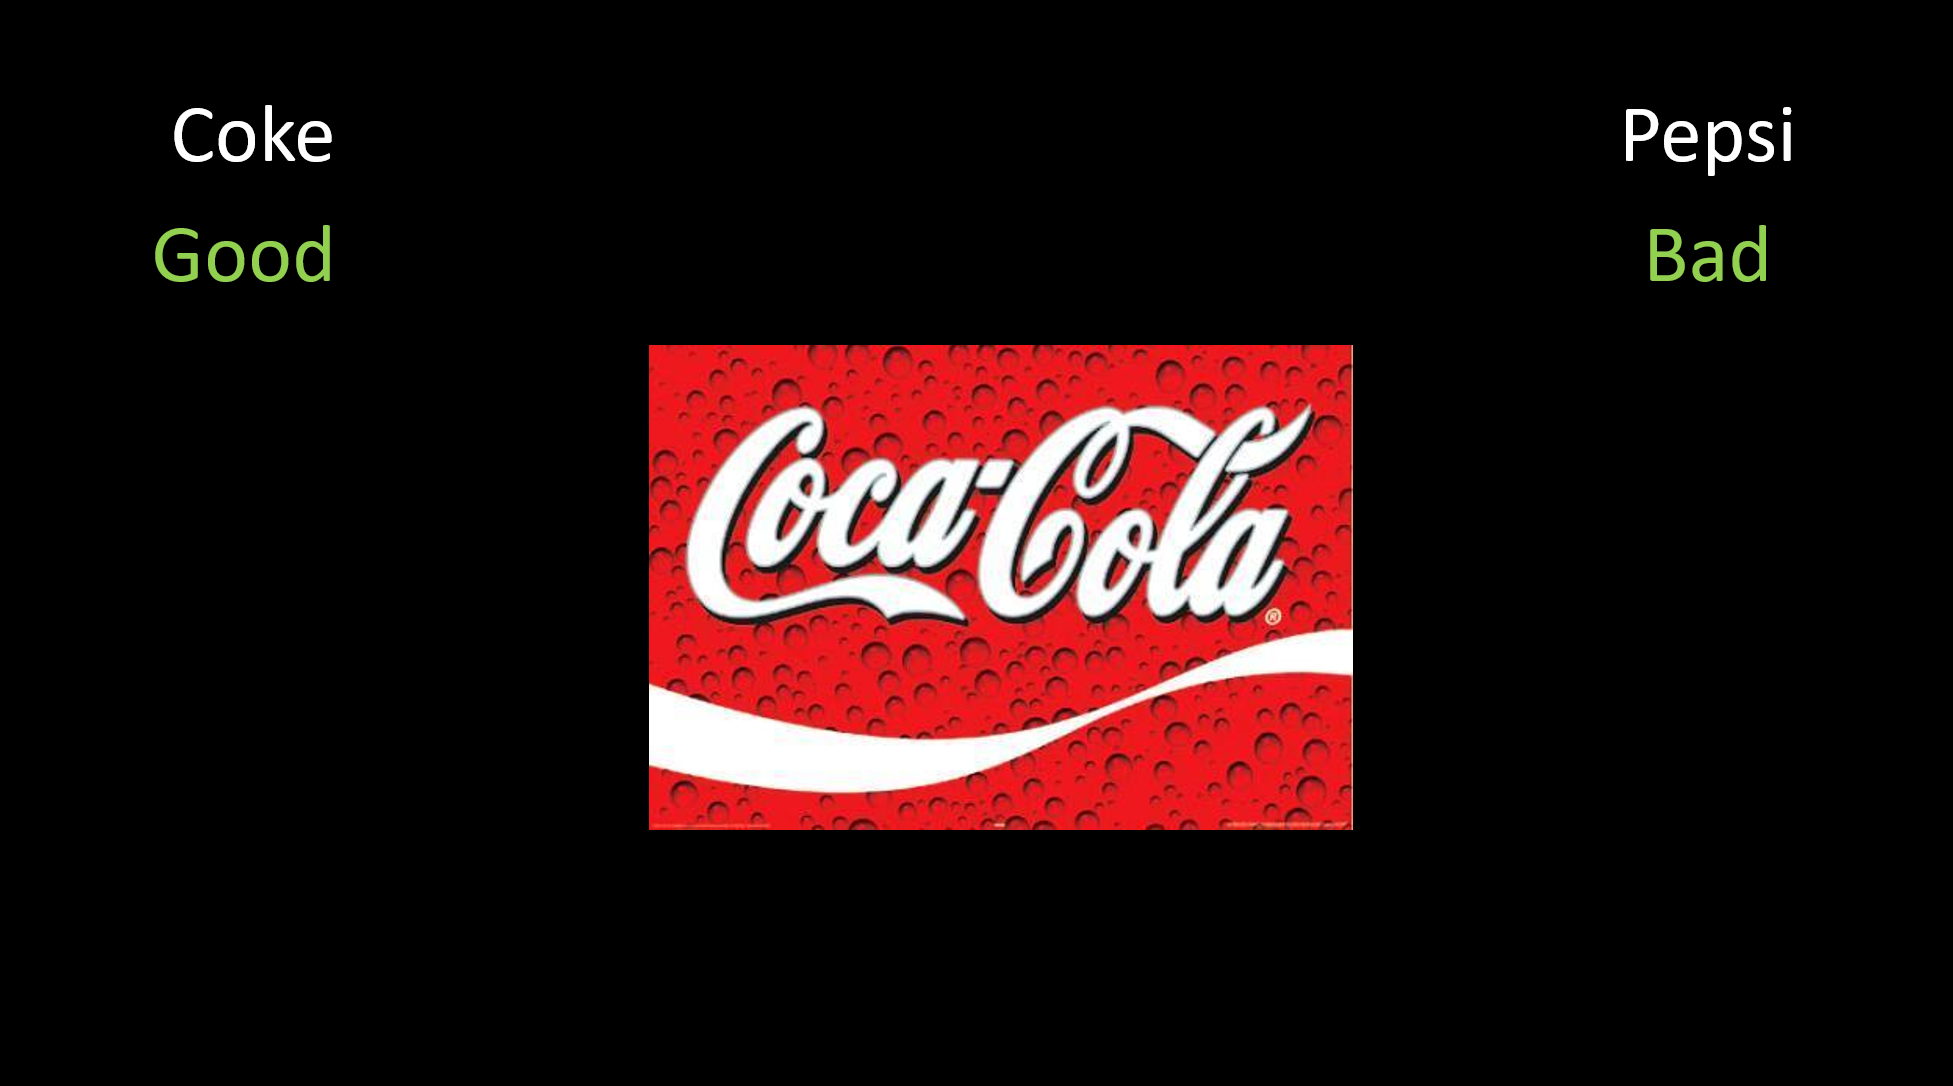
\includegraphics[width=\linewidth]{cocagood.png}
		\caption{Coke-Good/Pepsi-Bad condition}
		\label{cgpb}
	\end{subfigure}
	~ %add desired spacing between images, e. g. ~, \quad, \qquad, \hfill etc. 
	%(or a blank line to force the subfigure onto a new line)
	\begin{subfigure}[b]{0.4\linewidth}
		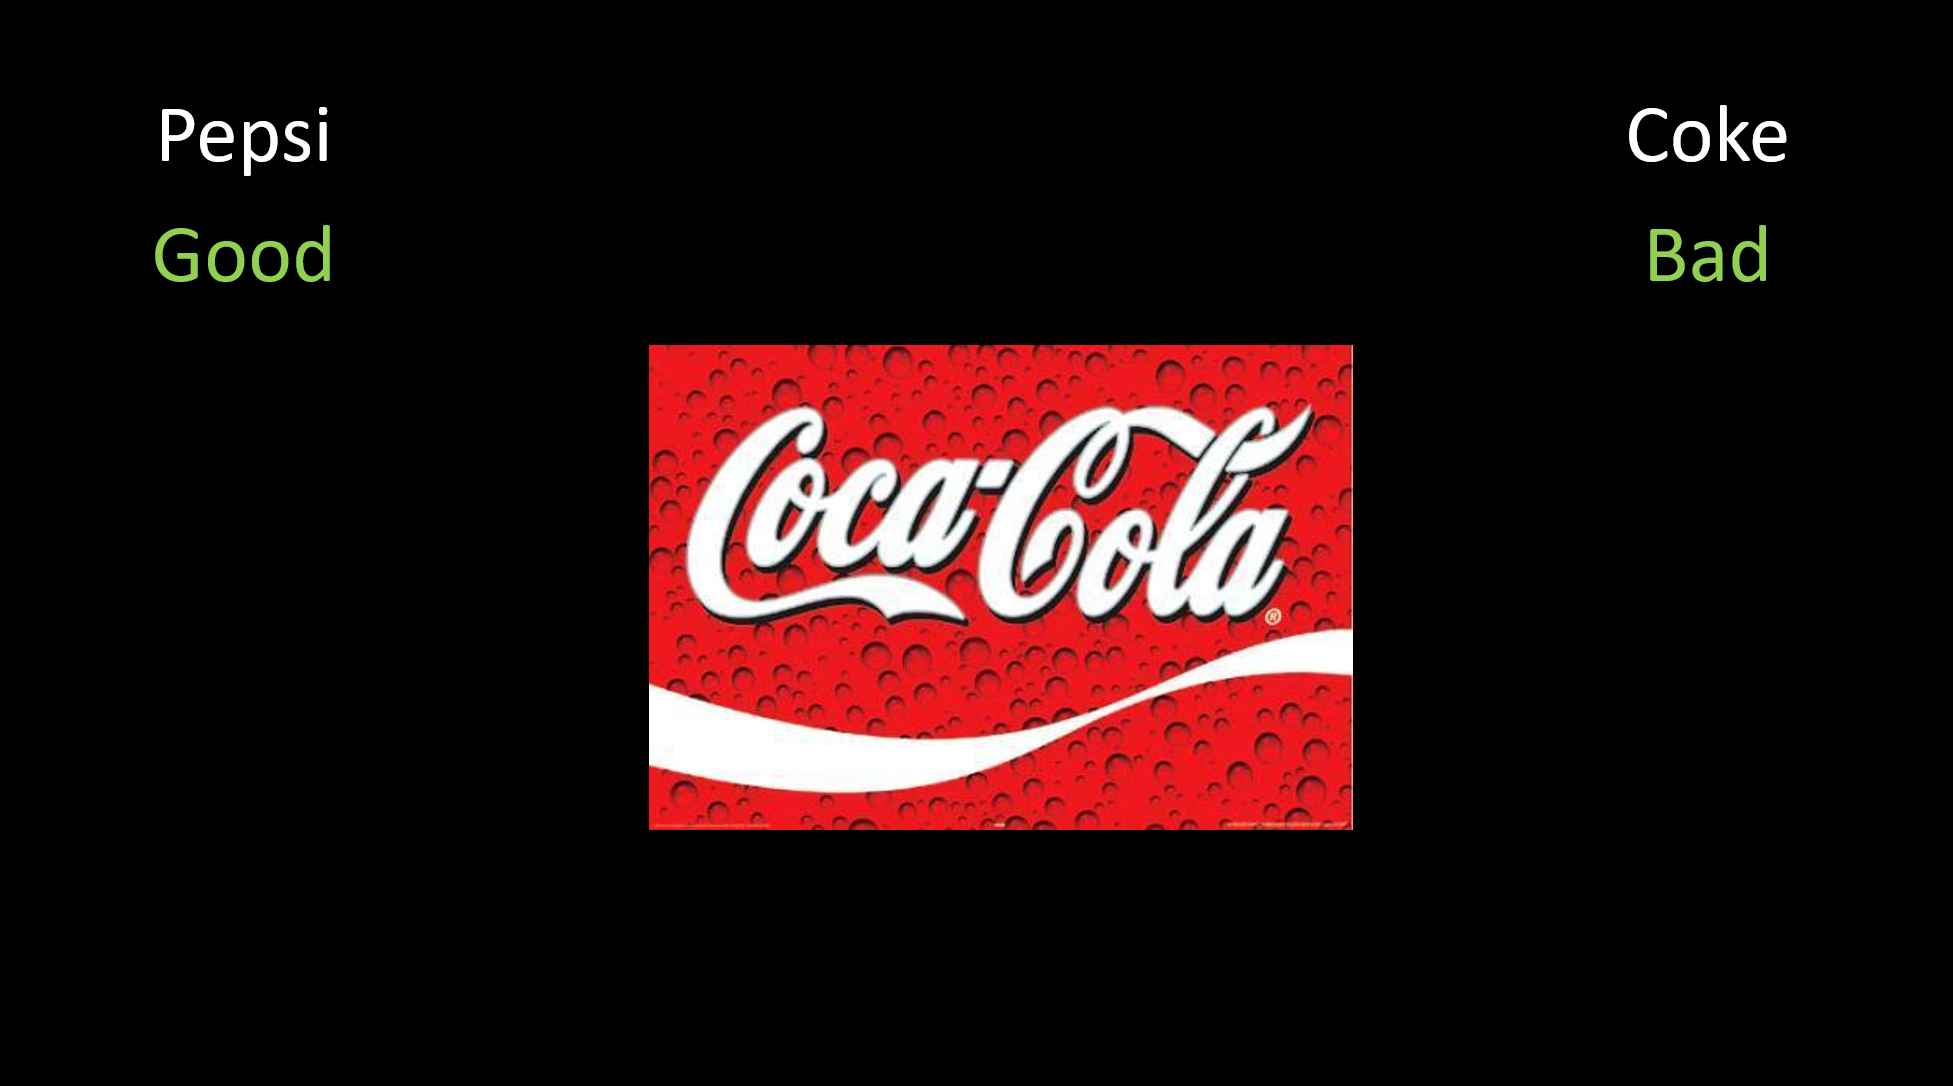
\includegraphics[width=\linewidth]{cocabad.png}
		\caption{Pepsi-Good/Coke-Bad condition}
	\end{subfigure}
	\caption{\label{fig:IAT} Associative conditions of a Coke-Pepsi IAT.}
\end{figure}



During the administration of the IAT, respondents might be given feedback of their performance. If the IAT administration includes the feedback presentation, a red ``X'' appears every time an incorrect response is registered (i.e., the stimulus is assigned to a category other than its belonging one). To proceed with the experiment, the respondents have to assign the stimulus to the category to which it belongs. When the IAT does not include feedback in the administration, respondents are not notified when they commit errors, and they keep going with the experiment. 



\subsection{Fields of application}

A recent literature review \cite{Epifania2020} showed an increased use of the IAT in wider and more varied fields of application.
Since the year of its first introduction (1998), the IAT has been used in more than 1,400 studies, investigating different topics. By reading the abstracts of the 1,418 papers citing and using the IAT (i.e., number of citations from 1998 to October 25\textsuperscript{th} 2019, date of the search on Scopus database), it was possible to identify 6 main fields of application of the IAT: Social psychology (i.e., studies aimed at the investigation of attitudes, their creations and change, regardless of the specific context, outgroup , or sample, $n = 513$), Clinical and personality psychology (i.e., studies aimed at the assessment of personality traits, both functional and dysfunctional, and mood disorders, $n = 290$), Addiction (i.e., studies on addiction, regardless of the substance, and the sample, $n = 113$) , Food research (i.e., studies on food perception and food preference, $n = 43$), Marketing research (i.e., studies on brand perception, decision making and brand preference, $n = $34), and Other applications (i.e., studies on all the topics not exhausted by the other macro-areas, $n = 425$). 
Figure \ref{fig:topicyear} depicts the trend lines of  each field of application from 1998 to 2019. 
\begin{figure}[!h]
	\centering
	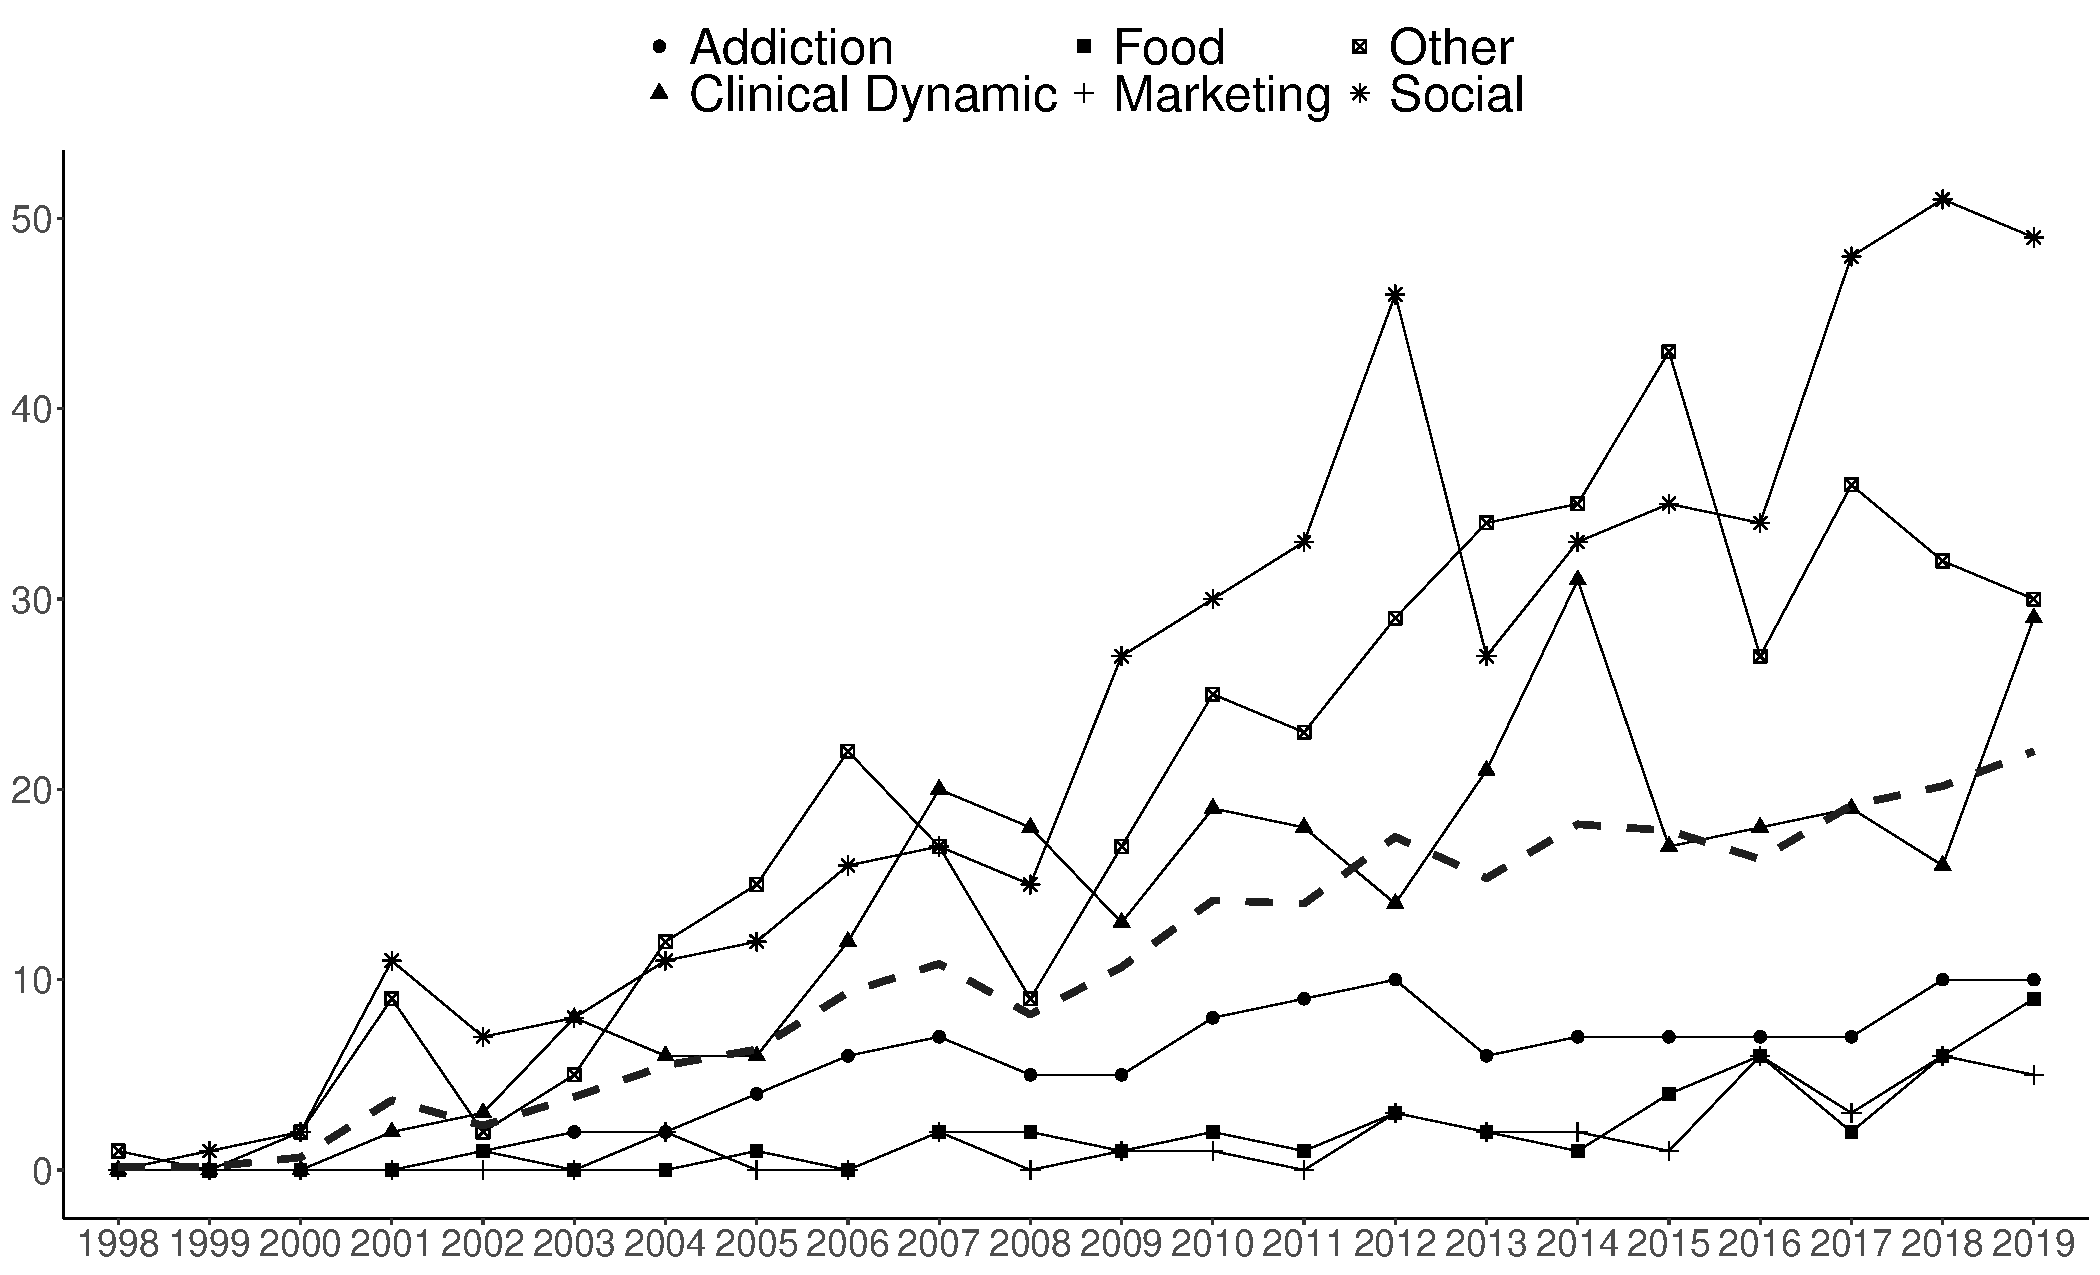
\includegraphics[width=\linewidth]{yearIATtopic.pdf}
	\caption{\label{fig:topicyear} Trend lines of each field of application of the IAT throughout from 1998 to 2019. }
\end{figure}
The dashed line in Figure \ref{fig:topicyear} represents the average trend of the IAT use across the fields of applications, pointing at a constant and on-going growth in IAT use throughout the years. 

The trend lines of the macro-areas Social psychology and Other appeared always above the mean trend line, while the trend line of the macro-area Clinical and personality psychology is the most inconsistent one throughout the years. 
The trend lines of the macro-areas Food and Marketing are similar between each other, and they both point at an increased use of the IAT in these fields during the past few years. 

Besides the general fields of applications of the IAT, it is interesting to delve deeper on the specific topics for which the IAT was employed (depicted in Figure \ref{fig:wordcloud}).

\begin{figure}[h!]
	\centering
	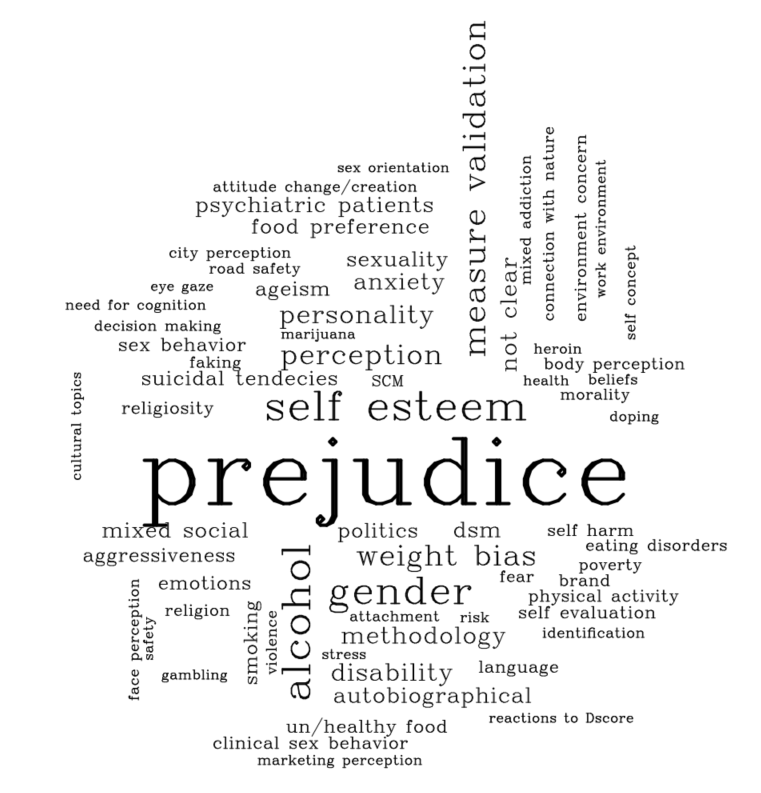
\includegraphics[width=0.5\linewidth]{wordcloudtopic.png}
	\caption{\label{fig:wordcloud} Word cloud of the fields of application of the IAT.  The bigger the word font, the more common the use of the IAT for the investigation of that specific topic.}
\end{figure}

Not surprisingly, the IAT was mostly used for investigating  implicit stereotypes and attitudes, such as implicit racial prejudice, gender stereotypes, attitudes towards obese people and other social groups (i.e., psychiatric patients and people with disabilities). 

The IAT has also been used for investigating addiction, unhealthy behaviors (i.e., smoking, alcohol consumption), personality traits, and self-perception.

The following paragraphs outline a brief summary of the IAT use in each field of application. The complete report of the fields of application of the IAT, along with the samples used in the studies, can be found in \citeA{Epifania2020}.

\paragraph{The IAT in the macro-area Social psychology.} The resistance of the IAT to self-presentation strategies \cite<e.g.,>{greenwald2009} made it particularly appealing for investigating socially sensitive topics, such as racial prejudice and, more generally, stereotypes and attitudes towards different out-groups. 
Studies on this topic are followed by studies focused on gender stereotypes, and on the investigation of illness-related attitudes. 
In this thesis, illness-related attitudes is a label used for indicating attitudes towards people with either mental or physical disabilities, psychiatric patients, people with HIV, cancer patients and patients in general, and suicide survivals.

Despite with lower frequency, the IAT is also used to assess attitudes towards people professing different religions, towards non-native English speakers, and bias towards people with low incomes. 
Papers composed of multiple studies in which attitudes towards multiple out-groups (e.g., out-group prejudice and weight bias) were concurrently investigated were common. The IAT was also used to investigate topics related to the Stereotype Content Model  \cite<SCM;>{fiske2002}, including infra-humanization, and to investigate the effectiveness of experimental manipulation to change/induce attitudes, even towards non-real groups.

\paragraph{The IAT in the macro-ares Clinical and personality psychology.} The IAT was mostly used for the implicit assessment of self-esteem. Personality traits (e.g., Big Five personality traits), anxiety, and personality and mood disorders according to Axes I and II of the Diagnostic and Statistical Manual of Mental Disorders (DSM) definition were fairly investigated as well. 
The IAT was also commonly used for the implicit assessment of suicidal tendencies, aggressiveness, emotions, and clinical sex behavior (e.g., pedophilia). 

\paragraph{The IAT in the macro-area Addiction.} The vast majority of studies using the IAT in this field were focused on the investigation of alcohol addiction, followed by studies on nicotine and smoking addiction. The concurrent investigation of multiple addictions, such as drinking with smoking or drinking with gambling, was quite uncommon. 

\paragraph{The IAT in the macro-area Food research.} The IAT was mainly used to investigate the preference for different kinds of food, the preference for healthy over unhealthy food, or food perception in general. The IAT was also employed for investigating attitudes towards dieting. Less common topics were food craving, food self--control, and the effect of the time of day on food preference. 

\paragraph{The IAT in the macro-area Marketing.} Marketing research is one of the most recent fields of applications of the IAT. Most of the studies are focused on the implicit evaluation of the preference between different brands. Additionally, the IAT has been employed for studying the processes driving the decision to purchase products, and the role of products labels and packaging in influencing the purchase of that specific product.

\paragraph{The IAT in the macro-area Other.} The studies included in this macro-ares cover a broad and extensive range of topics, from gender perception of odds and even numbers \cite{gendernumber} to work related stress \cite{workstress} and romantic attachment \cite{romantic}.
Studies aimed at the validation of the IAT are included as well, and they compose the vast majority of studies in this field of applications. They are followed by studies on human perception and studies on methodology. The distinction between measure validation papers and methodology papers is quite subtle. Measure validation studies include papers aimed at the validation of the IAT procedure \cite<e.g.,>{Greenwald1998}, its score \cite<e.g.,>{Greenwald2003}, and the factors that may affect the IAT effect \cite<e.g.,>{bluemke2006}. 
Methodology papers includes studies in which existing formal models were used for modeling IAT data, such as the application of the Many-Facet Rasch Measurement Model \cite{linacre1989} in \citeA{anselmi2011} or the application of the Diffusion Model \cite{ratcliff1978} in \citeA{Klauer2007}. Studies aimed at the validation of \emph{ad-hoc} models for IAT data, such as the Quad Model \cite{Conrey2005} or the Discrimination-Association Model \cite{stefanutti2013} are included under the label methodology as well.

\section{The Single-Category Implicit Association Test}\label{sec:sciat}

The IAT has vastly proven its effectiveness and usefulness in providing a relative measure of the preference towards one object category compared with a contrasted one. 
%Many attitudes or preference objects present a clear contrasted category, so that it is meaningful and useful to investigate the relative preference/attitudes \cite{greenwald2000}. 
However, the measure obtained from the IAT presents two main shortcomings.
%However, the relative measure provided by the IAT is not able to understand whether the performance is driven by a positive evaluation towards one of the objects, a negative evaluation towards the opposite one, or a combination of the two evaluations.
%The resulting IAT effect is not able to actually acknowledge for the specific preference/dislike driving the responses.
First, the relative measure provided by the IAT is not able to disentangle whether the performance is driven by a positive evaluation towards one of the objects, a negative evaluation towards the opposite one, or a combination of the two evaluations.
Sticking with the Coke-Pepsi IAT example in Section \ref{sec:iat}, faster responses in the Coke/Good-Pepsi/Bad associative condition might be due to either a preference for Coke (faster responses in sorting \emph{Coke} images and \emph{Good} attributes with the same response key), a dislike for Pepsi (faster responses in sorting \emph{Pepsi} images and \emph{Bad} attributes with the same response key), or even a combination of the two attitudes.  One could try to decompose the IAT effect by computing separate scores for the trials in which \emph{Good} attributes and \emph{Coke} (\emph{Pepsi}) images are associated and in which \emph{Bad} attributes and \emph{Coke} (\emph{Pepsi}) images are associated. Even by doing so, it is not possible to obtain an absolute measure of the preference towards one of the two beverages \cite{nosek2005}. The IAT is based on a comparative task and, as such, it can only result in a comparative measure.
Consequently, the IAT is not the most appropriate measure when the focus in on the assessment of the absolute positive or negative evaluation of a single object. 
Consider the implicit assessment of self-esteem.
In this instance, the interest would be on how much a person values himself/herself. 
However, studies that employed the IAT for implicitly investigating this construct contrasted the category \emph{Self} or \emph{Me} with a generic category, like \emph{Other} \cite<e.g.,>{selfesteemOther} or \emph{Not Me} \cite<e.g.,>{selfesteemME}. 
Consequently, the measure resulted in an indirect evaluation of how much a person valued himself/herself in comparison to others, and not in how much a person valued himself/herself \cite{karpinski2006}. 

Second, since the IAT effect depends on the relative evaluation between the two categories, the choice of the contrasted category is of the uttermost importance. In some cases, a clear contrasted category is not available, and the researcher has to make arbitrary choices. 
Sticking with the Coke-Pepsi IAT example in Section \ref{sec:iat}, the relative attitude towards Coke strongly depends on the attitude towards Pepsi (and vice-versa). For instance, a respondent indifferent to Coke but with a very strong dislike for Pepsi might result in a strong positive IAT effect. 
However, this effect would be mostly due to a dislike for Pepsi and not to a true positive evaluation of Coke. By replacing Pepsi with another soft drink, the resulting IAT effect for the very same respondent might change, and even result in a negative score.

Different alternatives have been introduced to overcome the issue of the relativeness of the IAT measure, such as the SC-IAT \cite{karpinski2006}. 
The SC-IAT results from a slight modification of the IAT procedure. It is aimed at assessing  the strength of associations between concepts by considering the speed and accuracy with which different stimuli are sorted in their reference categories. 
The assumption that underlies the functioning of the SC-IAT is the same as that underlying the functioning of the IAT, namely, that it is easier to sort together exemplars of two categories when they are strongly associated with each other than when they are not. However, differently from the IAT, the exemplars of only one object category (e.g., \emph{Coke} in a Coke SC-IAT), along with the exemplars of two evaluative dimensions, are presented. 
The usual structure of a SC-IAT is illustrated in Table \ref{tab:sciatstructure}. 
\begin{table}[h!]
	\centering \doublespacing
	\caption{Coke SC-IAT structure \protect\cite<adapted from >{karpinski2006}.}
	\label{tab:sciatstructure}
	\begin{tabularx}{\textwidth}{p{1cm} p{4cm} p{4cm} p{4cm}}
		\toprule
		Block  & Function  & Left Response key & Right Response key \\
		\midrule
		B1  & Associative practice & Good \& Coke & Bad \\
		B2  & Associative Test & Good \& Coke & Bad \\
		B3  & Associative practice & Good  & Bad \& Coke \\
		B4  & Associative Test & Good  & Bad \& Coke \\
		\bottomrule
		\multicolumn{4}{p{14cm}}{\onehalfspacing\emph{Note:} The order of presentation of Blocks B1 and B2 and Blocks B3 and B4 are counterbalanced across respondents.}
	\end{tabularx}
\end{table}
The SC-IAT is usually composed of 4 blocks. 
In the first two Blocks (B1 and B2), the target object \emph{Coke} and \emph{Good} attributes share the same response key, while \emph{Bad} attributes are sorted with the opposite response key (Coke/Good-Bad condition, CG). 
In the last two blocks (B3 and B4), target object \emph{Coke} is sorted with the same response key as \emph{Bad} attributes, while \emph{Good} words are sorted with the opposite response key (Coke/Bad-Good condition, CB).  
  
Blocks B1 and B3 are associative practice blocks, while Blocks B2 and B4 are the actual critical blocks that constitute the two associative conditions. 
%In the first critical block (B2), that is, the first critical condition, the target object \emph{Coke} and \emph{Good} attributes share the same response key, while \emph{Bad} attributes are sorted with the opposite response key (Coke/Good-Bad condition, CG). 
%In the contrasting associative condition (B4), target object \emph{Coke} is sorted with the same response key as \emph{Bad}, while \emph{Good} words are sorted with the opposite response key (Coke/Bad-Good condition, CB).  

The two conditions of the Coke SC-IAT described in Table \ref{tab:sciatstructure} are depicted in Figure \ref{fig:SCIAT}. 

\begin{figure}[h!]
	\centering
	\begin{subfigure}[b]{0.4\linewidth}
		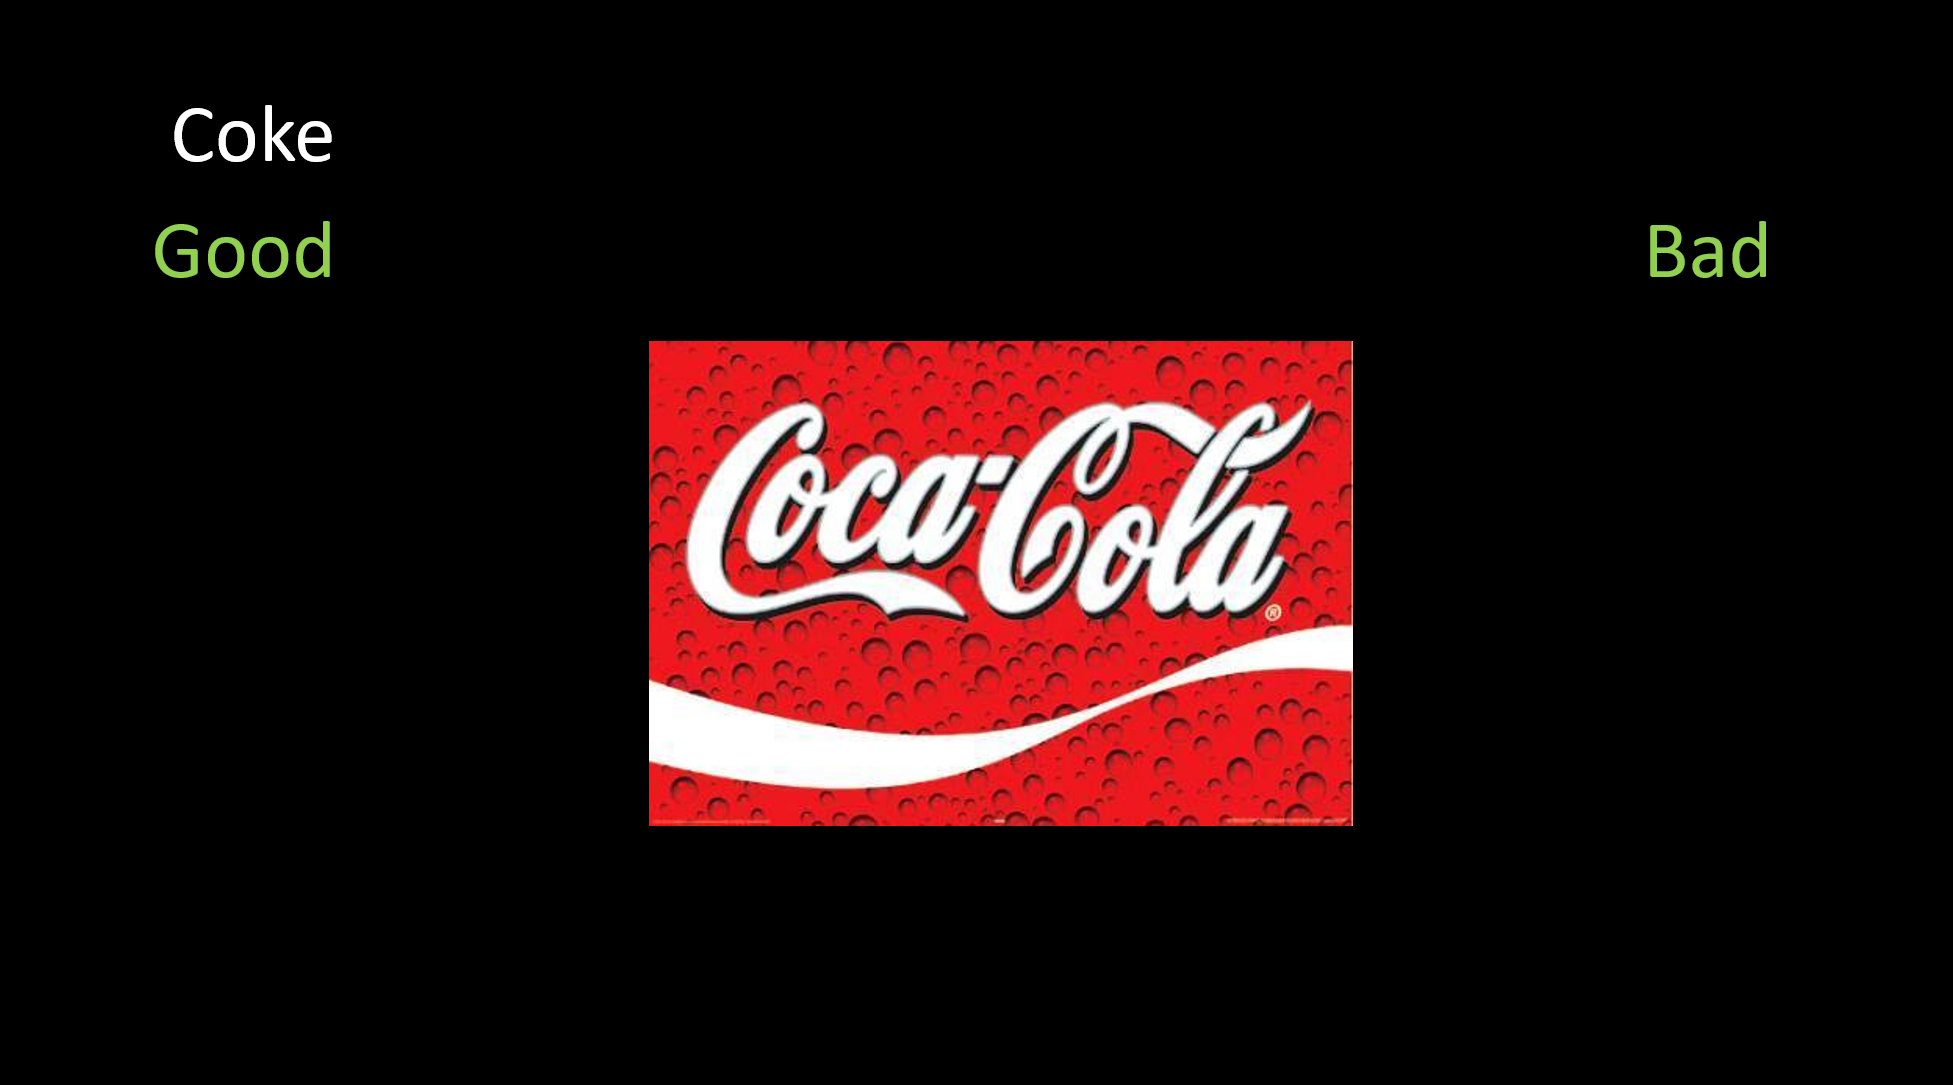
\includegraphics[width=\linewidth]{sccokegood.png}
		\caption{Coke-Good/Bad condition}
	\end{subfigure}
	~ %add desired spacing between images, e. g. ~, \quad, \qquad, \hfill etc. 
	%(or a blank line to force the subfigure onto a new line)
	\begin{subfigure}[b]{0.4\linewidth}
		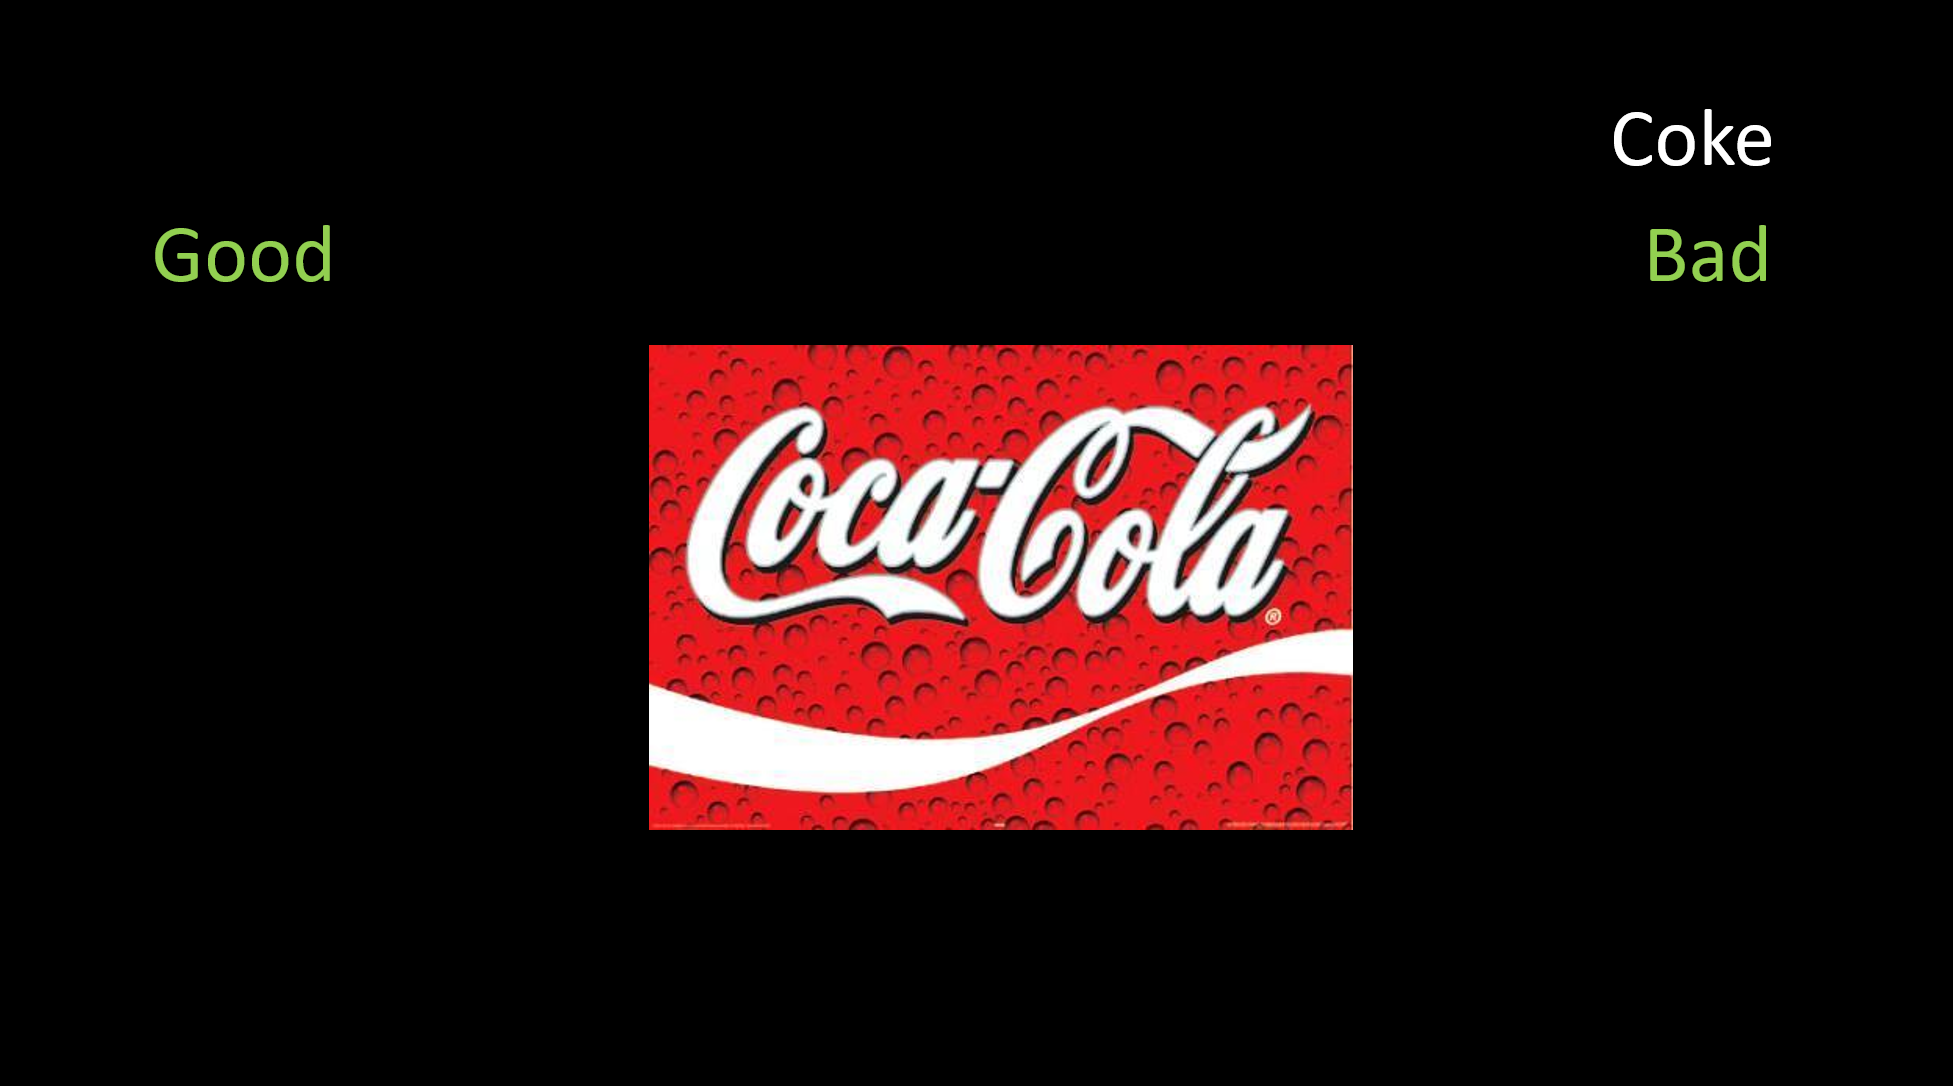
\includegraphics[width=\linewidth]{sccokebad.png}
		\caption{Coke-Bad/Good condition}
	\end{subfigure}
	\caption{\label{fig:SCIAT} Associative conditions of a Coke SC-IAT.}
\end{figure}

The SC-IAT administration usually includes a response time window (rtw) at 1,500 ms, after which the stimulus disappears and a warning message (e.g., ``Respond more quickly!'') is given to the respondent.
Every correct response is signaled by a green ``O'', while every incorrect response is signaled by a red ``X''. Differently from the IAT, respondents do not have to correct their incorrect responses to go on with the experiment. 

The rtw and feedback for every response differentiate the SC-IAT from the Single Target IAT \cite<ST-IAT;>{stiat}. Nonetheless, the names (and procedures) of the two measures are used interchangeably \cite<e.g.,>{bar2014}.
The SC-IAT effect results from the difference in respondents' performance between the two contrasting conditions, and it is usually expressed by a modification of the IAT \emph{D} score algorithm \cite[see Section \ref{sec:sciatD}]{karpinski2006}.

\section[Fully-crossed design]{The fully-crossed design of implicit measures}\label{sec:cross}

Suppose that two respondents, Lara and Francesco, are presented with the Coke-Pepsi IAT in Section \ref{sec:iat}. 

On average, Lara might be more accurate (or faster) than Francesco. 
The difference in the overall performances of Lara and Francesco  is ascribable to their individual differences and their characteristics. 
The between--respondents variability is the expression of the differences due to these individual characteristics, irrespective of the associative conditions. 

The set of exemplars chosen for representing each category presents their own variability as well. 
The \emph{Coke} logo can be immediately recognized and sorted in its own category, while an image of an old fashioned can of Coke might be less familiar and hence might need more time for being recognized and sorted. 
Similarly, the attribute \emph{evil} might be immediately recognized as belonging to the evaluative dimension \emph{Bad}, while the attribute \emph{wicked} might not be immediately recognized as belonging to the evaluative dimension \emph{Bad} \footnote{The attribute \emph{evil} is the English translation of the Italian word \emph{cattivo}. The attribute \emph{wicked} is the English translation of the Italian word \emph{malvagio}. 
	The spread Index (which varies from 0 to 1, where 1 indicates a high spread) for the former one is 0.85, while for the latter is 0.36 \cite{colfis}, indicating that the  word \emph{cattivo} (\emph{evil}) is more spread and used than the word \emph{malvagio} (\emph{wicked}). As such, the meaning of the former word might be more familiar than the meaning of the latter one (in Italian).}. 
The between--stimuli variability is the expression of the sampling variability due to stimuli characteristics, irrespective of the associative conditions. 

So far, only the between--respondents variability and the between--stimuli variability have been considered as the expression of the individual and stimulus differences, respectively.
The effect of the IAT associative condition has not been mentioned yet. Nevertheless, the main object of investigation in IAT studies is the variation in the performance of the respondents between the associative conditions.

The individual differences of the respondents might be exacerbated or diminished by the effect of the associative condition. 
Recall that Lara showed a better overall performance than Francesco. 
However, the difference in their performances might be attenuated in the Coke-Good/Pepsi-Bad condition, potentially due to several reasons. 
For instance, Lara might keep her performance unaltered because she is neither fond of Coke nor disgusted by Pepsi, while Francesco might show a better performance because he particularly likes Coke over Pepsi. 
In the opposite condition, the difference between the performances of Lara and Francesco might be exacerbated. Lara might still keep her performance unaltered, while Francesco might struggle in associating his favorite soda with negative attributes. 
The within--respondents between--conditions variability is hence the expression of the variability in the performance of the respondents ascribable to the effect of the associative condition. 
Usually, to investigate whether the associative condition had an effect on the performance of the respondents, a \emph{by-participant} approach is undertaken \cite<i.e., a score for each respondent is obtained by taking the difference between the across-trial average response time in each condition;>{judd2012}.

There are no reasons to suppose that stimuli are immune to the effect of the associative condition. 
Some of the stimuli might be more easily sorted in one associative condition than the other for a number of reasons, including the specific attitudes of the respondents. 
The within--stimuli between--conditions variability indicates whether the  functioning of the stimuli changes according to the associative condition in which they are presented. 
By exploiting this information, it is possible to obtain a measure of the contribution given by each stimulus to the IAT effect. The more (less) a stimulus functioning changes between the conditions, the higher (lower) its contribution to the IAT effect. 
Often, to investigate the effect of an experimental variable on the functioning of the stimuli a \emph{by-stimulus} approach is undertaken \cite<i.e., a score for each stimulus is obtained by taking the difference between the across-respondents average response time in each condition;>{judd2012}. 

One source of variability (i.e., the variability due to the reactions of each respondent to each stimulus) has not been mentioned yet.
Lara is a better respondent than Francesco, but she also does not have a particular preference for any of the sodas. As such, Lara might generally react in the same way to each of the stimuli representing the two brand of sodas. 
On the other hand, Francesco has a strong preference for Coke. As such, he might be more able than Lara in recognizing even the above-mentioned old-fashioned can of Coke. 
Consequently, he would have a better performance than Lara on this specific stimulus. 
The interaction between the respondent and stimulus variabilities is the expression of the interaction between the respondent and stimulus characteristics. 

This practical example provided a clear overview of how the sources of variability in the IAT data are generated, and it can be used as a starting point for further illustrating the IAT data structure and its sources of random variability. 

In the IAT\footnote{The SC-IAT presents the same data structure, although one of the target categories is dropped.}, the respondents are presented multiple times with the stimuli nested in two levels of two independent variables, namely the evaluative dimensions (\emph{Good} vs \emph{Bad}) and the target objects (e.g., \emph{Coke} vs \emph{Pepsi}). In a multilevel modeling perspective, the respondents and the stimuli can be considered at the same level.
%Since respondents are presented multiple times with the stimuli representing each of these categories, they are crossed with each level of the independent variables. Individual stimuli and individual respondents are at the same level and they are crossed with each other. 

The associative conditions constitutes another independent variable, composed of two levels (e.g., the CGPB and PGCB associative conditions of the Coke-Pepsi IAT). 
Being at a higher level, this variable includes both the respondents and the stimuli, and its effect on the performance of the respondents is usually the main focus of investigation in IAT studies. 

The stimuli representing each of the categories are presented multiple times to the respondents both within and between the associative conditions. 
As such, the stimuli are crossed with both the respondents and the associative condition. 
%Similarly, the respondents are presented multiple times with the stimuli, both within and between the associative conditions. Therefore, also the respondents are crossed with the stimuli and the associative condition. 
Besides being crossed with each other, the respondents and the stimuli are both crossed with the associative conditions \cite<fully-crossed design;>{Westfall2014}.
%This data structure is usually referred to as a fully-crossed design, where all the levels of the independent variables are crossed with each other \cite{Westfall2014}. 

The responses $x_{ps}$ of three participants $p_p$ to three stimuli $s_s$ (i.e., \Cat, \Snowman[1.5], \NiceReapey) in the two IAT associative conditions $c$ are represented in Table \ref{tab:fully} to exemplify the fully-crossed structure characterizing the measure.  
\begin{table}[h!]
	\caption{Fully-crossed design.}
	\label{tab:fully} \centering \onehalfspacing
	\begin{tabular}{p{1cm} p{0.05cm} p{1.5cm} p{1.5cm} p{1.5cm} p{0.05cm} p{1.5cm} p{1.5cm} p{1.5cm}}
		\toprule
		& \multicolumn{3}{c}{Condition A} & & \multicolumn{3}{c}{Condition B}\\
		\midrule
		\multirow{2}{*}{$p_1$} &  \multicolumn{1}{|c}{} & \Cat[2] & \Snowman[2.5] & \NiceReapey[2] & &  \Cat[2]  & \Snowman[2.5] & \NiceReapey[2] \\
		&  \multicolumn{1}{|c}{} & \Cat[2] & \Snowman[2.5] & \NiceReapey[2] & & \Cat[2] & \Snowman[2.5] & \NiceReapey[2] \\
		\hline
		\multirow{2}{*}{$p_2$} &  \multicolumn{1}{|c}{} & \Cat[2] & \Snowman[2.5] & \NiceReapey[2] & & \Cat[2] & \Snowman[2.5] & \NiceReapey[2] \\
		& \multicolumn{1}{|c}{} & \Cat[2] & \Snowman[2.5] & \NiceReapey[2] & & \Cat[2] & \Snowman[2.5] & \NiceReapey[2] \\
		\hline
		\multirow{2}{*}{$p_3$} & \multicolumn{1}{|c}{} & \Cat[2] & \Snowman[2.5] & \NiceReapey[2] & & \Cat[2] & \Snowman[2.5] & \NiceReapey[2] \\
		& \multicolumn{1}{|c}{} & \Cat[2] & \Snowman[2.5] & \NiceReapey[2] & & \Cat[2] & \Snowman[2.5] & \NiceReapey[2] \\
		\bottomrule
		\multicolumn{8}{p{10cm}}{\emph{Note:} $p$: Respondents.}
	\end{tabular}
\end{table}
Each cell of Table \ref{tab:fully} contains the unique combination respondent $\times$ stimulus for every repetition of the stimulus in each associative condition ($x_{psc}$, the response to each  trial of the IAT). 
The trials of the IAT are at the lowest level of observation resulting from the crossing between the stimuli, the respondents, and the associative conditions.
The illustration in Table \ref{tab:fully} represents how the dependency at the level of the single observations is generated by the random noise in the data. 

Data deriving from a fully-crossed design, such as that of the IAT, should be carefully analyzed to account for the sources of variability related to the participants, the stimuli, the associative conditions, and their interactions \cite{Baayen2008, Barr2013, judd2017,  Westfall2014, wols2017}.  
These sources of variability generate dependencies between the observations that violate the assumption of conditional independence. 
This assumption is the basic assumption underlying data analysis in Social sciences, according to which, once the effect of the variability due to one latent variable is accounted for, the remaining variability can be explained by means of the experimental factors.
Conditional independence is often referred to as local independence as well. The two terms are used interchangeably throughout the thesis.

%As depicted in Table \ref{tab:fully}, the fully-crossed design characterizing the IAT (SC-IAT) results in a unique combination respondent $\times$ stimulus for every repetition of the stimuli in each associative condition, and different  sources of variability and dependency in the observed responses -- related to participants, stimuli, conditions, and to their interaction -- should be expected \cite{Barr2013, Westfall2014, wols2017}. 



%These are the main sources of variability that can be found in IAT or SC-IAT data and that have to be accounted for in order to obtain reliable estimates. 
%However, there is a part of variability that is due to the reactions of each respondent to each stimulus 
%Nonetheless, there's still a part of variability that is left out, which is the variability due to the presentation of each stimulus to each participant, or, in other words, the reaction of each respondent to each stimulus. 
Usually, the IAT (or SC-IAT) effect is expressed by an effect size measure obtained by aggregating the responses across the trials in each associative condition, and dividing these quantities by the standard deviation computed on the pooled trials of both blocks. 
These measures are the so-called \emph{D} score \cite<Chapter \ref{chap:classicscore};>{Greenwald2003, karpinski2006} that provide an easy-to-compute and easy-to-interpret measure of the bias assessed by the implicit measure. 

However, the easiness with which the \emph{D} score is computed and interpreted comes with drawbacks that cannot be ignored. 
The computation procedure of the \emph{D} score implicitly entails that the stimuli are taken as the exhaustive representation of the population of stimuli (i.e., fixed factors), while the respondents are considered as just one of the possible samples that can be drawn from a population (i.e., random factors) \cite{judd2012}. 
Assuming that the respondents are random factors (to be treated as random effects) and the stimuli are fixed factors (to be treated as fixed effects) defines a \emph{by-participant} analysis. 
However, taking the stimuli as fixed factors has important consequences, both theoretically and statistically. 
Firstly,  all the stimuli are assumed to have the same functioning and the same effect on the observed measure.
Moreover, only inferences concerning the population of the respondents are allowed. As such, the results are generalizable at the respondent level and their replicability  is bounded to the use of the same exact set of stimuli \cite{judd2012}. 
Finally, by averaging across the trials in each condition, the between--stimuli variation is left uncontrolled. As such, all the information that can be gathered from the stimuli is lost \cite{wols2017}.  
Moreover, when the unaccounted by-stimulus variation is confounded with the effect of interest (the effect of the IAT associative conditions), the risk of committing Type I error is inflated, and any significant difference between the means can be due to the sources of error variance and not to the experimental effect \cite{Barr2013, judd2012,mc1989}. 
Not accounting for the sources of error variance has important consequences also when the uncontrolled source is orthogonal (i.e., independent) to the effect of interest. In this case, the un-controlled error variance reduces the power for testing the relevance of the effect of interest. Consequently, the importance of the experimental manipulation is underestimated \cite{Barr2013}. 

%In the IAT (SC-IAT) case, the investigation at the stimulus level is not aimed at the functioning of each individual stimulus. Rather, the aim is to gather the information provided by each of the stimulus categories. Since the individual stimulus is taken to be the manifestation of its own category, the stimuli of the IAT (SC-IAT) can be conceptualized as samples drawn from the populations defined by their belonging category \cite{wols2017}.
%As such, it makes sense to conceptualize the stimuli used in an IAT (SC-IAT) as possible samples drawn from the populations defined by the category to which they belong \cite{wols2017}. 
%Given this conceptualization, considering stimuli as fixed factors and not accounting for their sampling variation appear to be great fallacies when treating IAT (SC-IAT) data. 
%Moreover, when the by-stimulus variation is not accounted for, all the information that can be gathered from them is overlooked \cite{wols2017}.
% the response given to a single, individual stimulus is not important \emph{per se}. Rather, the interest is on the categories that the stimuli are supposed to represent, with each individual stimulus being a realization of its category. The stimuli used in an implicit measure can be conceptualized as drawn from the population of stimuli representing their belonging category \cite{wols2017}. Moreover, by overlooking the sampling variation related to the stimuli, the information that can be gathered from them is completely neglected \cite{wols2017}.

Potentially, the between--stimuli variability can be accounted for by performing \emph{by-stimulus} analyses \cite{judd2012}. 
Differently from the \emph{by-participant} approach (respondents are treated as random factors and stimuli as fixed factors by averaging per participant across stimuli), the \emph{by-stimulus} approach treats the stimuli as random factors and the participants as fixed factors by averaging per stimulus across participants. 
The stimuli are hence taken to be just one of the possible sets of stimuli that can be drawn from a population of stimuli. 
Clearly, the same pitfalls highlighted for the \emph{by-participant} approach apply for this instance, but reversed. 
Not considering the between--participants variability affects the computation of the mean score for each stimulus and the results of the statistical tests that are performed.  
However, the \emph{by-stimulus} analyses allow for the generalization of the results at the stimulus level, and  inferences can be made on the population from which the stimuli are drawn. This makes the results replicable with other sets of stimuli drawn from the same population, but only if they are administered to the same sample of respondents \cite{judd2012}. 

As an attempt to overcome the replicability and generalizability issues concerning either the \emph{by-participant} approach or the \emph{by-stimulus} one, \citeA{raaijmakers1999} suggested to report the results obtained with both the \emph{by-participant} and the \emph{by-stimulus} analyses. The results are accepted as significant only if both the analyses yield significant results. 
The underlying logic appears to be quite straightforward. 
Given that the \emph{by-participant} analysis allows for generalizing to other populations of respondents (but only if the same stimuli are employed) and the \emph{by-stimulus} analysis allows for generalizing to others population of stimuli (but only if the same sample of respondents is used), if they are both significant it is possible to generalize across both of them (i.e., to new samples of respondents and to new samples of stimuli concurrently).
Quite blatantly, this approach cannot do what it claims to do \cite{raaijmakers1999, raaijmakers2003}. 
The \emph{by-participant} analysis keeps ignoring the sampling variation of the stimuli and the \emph{by-stimulus} analysis keeps ignoring the sampling variation of the respondents. As such, their results are still flawed by uncontrolled sources of error variance.
Besides, this approach presents also theoretical fallacies. 
%Significant \emph{by-participant} results do suggest would replicate only if the same set of stimuli is used. 
%Conversely, significant \emph{by-stimulus} results would replicate only if the same sample of respondents is used. 
The syllogistic reasoning according to which if both the premises are true (both the \emph{by-participant} and the \emph{by-stimulus} analyses are simultaneously significant and hence the results can  be replicated on different samples of respondents and stimuli, respectively) then also their conjunction would hold true (i.e., the results can be replicated on new samples of respondents and stimuli concurrently) appears too bold. 

A solution to this impasse is to consider both the respondents and the stimuli as random factors. 
By doing so, all the sources of variability at different levels and their potential interactions can be accounted for, resulting in more reliable estimates \cite{Barr2013, judd2012, wols2017}.
Moreover, considering the respondents and the stimuli as random factors implies that both levels are assumed to be drawn from larger populations \cite{judd2012, wols2017}. 
While the implications of treating the respondents as random factors are immediately clear, since they are typically considered as samples drawn from larger population, the same cannot be said for the stimuli. 
Treating stimuli as random factors entails that their functioning can vary for each observational unit. Consequently, they can differently affect the observed measure, and their functioning and relevance to the observed measure can be directly investigated \cite{judd2012}.  
Assuming that all the employed stimuli in the IAT have the same effect on the outcome measure (i.e., the difference in the average response time in each associative condition) is an already proved fallacy \cite<e.g.,>{bluemke2006, ellithorpe2015}. As such, both the stimuli and the respondents should be considered as random factors for a meaningful and reliable analysis of the IAT data. 

The scores presented in Chapter \ref{chap:classicscore} are all affected by the above mentioned issues, as well as the formal models for the analysis of the IAT data presented in Chapter \ref{chap:formalModel}. 
The approach used to address the fully-crossed structure of the IAT is presented in Chapter \ref{chap:modelsIAT}.


\subsection{More than one implicit measure}
It is not uncommon to find studies in which the IAT and the SC-IAT are used concurrently to obtain both a comparative measure of the attitudes towards one object in comparison to its opposite, as well as an absolute measure of the positive/negative evaluations towards each of them  \cite<e.g.,>{bulmer2018implicit, fairer, glashouwer2013low}. 
To pursue this aim, one IAT and two SC-IATs, one for each of the target objects, are administered to the same respondents. The data of each implicit measure are analyzed separately by computing individual scores for each measure, which are  employed for further analysis.

When both implicit measures are administered together, the fully-crossed structure represented in Table \ref{tab:fully} is repeated for each of them. 
Each implicit measure comes with its own sources of variability due to its fully-crossed structure.
Moreover, a super-ordinate variable above the associative condition is added. The new super-ordinate variable is the type of measure. 
The associative conditions are hence nested within the specific implicit measure, while the respondents, besides being crossed with the stimuli and the measure-specific associative conditions, are also crossed with the implicit measures. Moreover, since the same stimuli are usually employed to represent the target objects and the evaluative dimensions in all implicit measures, also the stimuli are crossed with the implicit measures.
However, not all the stimuli are crossed with all implicit measures. While the stimuli belonging to the evaluative dimensions are crossed with all implicit measures (i.e., they are administered in all implicit measures), the stimuli representing the target objects are presented only according to the specific measure. 
Specifically, stimuli representing both target objects are presented in the IAT, while only one of the target object categories is presented in each SC-IAT. The variable type of measure hence introduces a nesting related to the stimuli. 

The implicit measure tends to be a variable of interest only in studies aimed at either the validation of the measure itself or at the investigation of their different functioning.
Nevertheless, the by-measure variability that has been introduced needs to be taken into account to obtain reliable estimates and scores.

%When the IAT and the SC-IAT are administered together, each of them comes with its sources of dependence and variability due to the fully-crossed design characterizing each of them. 
%Moreover, if the IAT and the SC-IAT are administered with a \emph{within--subject} design, other sources of variability and dependency affect the data. 
%Firstly, the administration of each measure to the each respondent generates a variability within the responses of the same individual and between the implicit measures considered. This variability reflects the impact of each implicit measure on respondents' performance. 
%Moreover, since the same stimuli are usually employed for representing both the evaluative dimensions and the target object(s) in each measure, a within--stimuli between--measures variability should be expected as well. The within--stimuli between--measures variability should be considered as an indicator of a different functioning of the stimuli according to the specific implicit measure in which they have been presented. 

If the by-measure variability is left unaccounted, the scores computed on each implicit measure include the sources of random variation due to both the fully-crossed design of each measure and the variability that should be expected by the multiple administration of the same set of stimuli to the same sample of respondents. 
The approach aimed at overcoming these issues with a comprehensive modeling of multiple implicit measures is presented in Chapter \ref{chap:comprehensiveModels}.

\chapter{Typical scoring of implicit measures}\label{chap:classicscore}
This chapter presents the scoring procedures for the IAT and the SC-IAT data and the development of new open source tools for easily scoring the IAT and the SC-IAT.

It is not unusual to find studies in which both the IAT and the SC-IAT are administered together, and their predictive performances in respect to different criteria are compared. 
However, this comparison might be biased by many differences concerning both the administration and the scoring procedures of the two implicit measures. 
Therefore, new scoring algorithms are introduced with the aim of reducing the noise due to external factors (i.e., the scoring procedure itself) in the comparison between implicit measures. 
The results of an empirical study in which the performance of typical and modified scoring algorithms have been compared in respect to the prediction of a behavioral outcome are reported.

The core computation of both the IAT and the SC-IAT scores is rather easy. Nonetheless, the many steps that have to be undertaken for preparing and cleaning the data make it an error-prone procedure, and compromise the reproducibility of the results. Since there is a lack of easy-to-use and open source tools for their computation, a Shiny app and an \verb*|R| package have been developed for the computation of the IAT and the SC-IAT \emph{D} scores. These tools are presented at the end of the chapter.

\section{The IAT \emph{D} score}\label{sec:iatD}
\citeA{Greenwald2003} introduced different variations of the \emph{D} score algorithm (Table \ref{tab:Doverview}), resulting from the combination of the error correction strategy (``Error replacement'' in the table) and the treatment for fast responses (``Lower tail treatment'' in the table).
\begin{table}[th!]
	\centering \doublespacing
	\caption{\label{tab:Doverview} Overview of the typical \emph{D} score algorithms. }
	\begin{tabularx}{\textwidth}{p{4cm} p{4cm} p{4cm}}
		\toprule
		Algorithm & Error replacement & Lower tail treatment\\\hline
		\emph{D}1 & Built-in correction & No \\
		\emph{D}2 & Built-in correction & Delete trials $<$ 400ms \\
		\emph{D}3 & Mean $+$ 2\emph{sd} & No\\
		\emph{D}4 & Mean $+$ 600ms & No \\
		\emph{D}5 & Mean $+$ 2\emph{sd} & Delete trials $<$ 400ms\\
		\emph{D}6 & Mean $+$ 600ms & Delete trials $<$ 400ms \\
		\bottomrule
		\multicolumn{3}{p{\textwidth}}{\onehalfspacing\emph{Note:} For all algorithms trials with a latency $>$ 10,000 ms are discarded. For the algorithms in which incorrect responses are replaced with the average response time inflated by a fixed penalty, the average response time is computed on the correct responses only.}
	\end{tabularx}
\end{table}

Blocks B1, B2, and B5 in Table \ref{tab:iatstructure} are considered as pure practice blocks and are discarded from the computation. Only trials from Blocks B3, B4 (i.e., Mapping A) and B6, B7 (i.e., Mapping B ) are used for the computation.  

The error correction strategies based on built-in correction (\emph{D1} and \emph{D2} in Table \ref{tab:Doverview}) refer to the IAT procedure including feedback, according to which  respondents have to correct their incorrect responses to continue with the experiment. 
The response time considered for the computation of the \emph{D} score is the response time at the first (incorrect) response inflated by the time required to correct it. All other algorithms (from \emph{D1} to \emph{D6} in Table \ref{tab:Doverview}) use a \emph{post-hoc} error correction strategy, for which the incorrect responses are replaced by the average response time of the correct responses in the block in which the error occurred increased by a standard penalty (i.e., either 600 ms or twice the standard deviation).
The other feature differentiating the \emph{D} score algorithms is the lower tail treatment, according to which fast trials (trials faster than 400 ms) are discarded or not.

Regardless of the specific features of each algorithm, the core procedure for computing the \emph{D} score is the same. Firstly, the \emph{D} scores of the associative practice blocks (Eq. \ref{eq:practice}):
%
\begin{equation}\label{eq:practice}
	D_{\text{practice}} = \frac{M_{\text{B6}} - M_{\text{B3}}}{\text{\emph{SD}}_{\text{B6, B3}}}, 
\end{equation}
%
and of the associative test blocks (Eq. \ref{eq:test}):
%
\begin{equation}\label{eq:test}
	D_{\text{test}} = \frac{M_{\text{B7}} - M_{\text{B4}}}{\text{\emph{SD}}_{\text{B7, B4}}},
\end{equation}
are computed.
In both cases, the difference in the average response time between the two critical blocks is divided by the standard deviation computed on the pooled trials of both blocks. Once the $D_{\text{practice}}$ and the $D_{\text{test}}$ are obtained, it is possible to compute the actual \emph{D} score: 
%
\begin{equation}\label{eq:dscore}
	\text{\emph{D} score} = \frac{D_{\text{practice}} + D_{\text{test}}}{2}.
\end{equation}
The block order in Equation \ref{eq:practice} and Equation \ref{eq:test} is arbitrary and can be reversed. The resulting \emph{D} has to be interpreted accordingly. 
In the Coke-Pepsi IAT in Chapter \ref{chap:intro}, Blocks B3 and B4 constituted the Coke-Good/Pepsi-Bad condition. 
Conversely, the Pepsi-Good/Coke-Bad condition was composed of Blocks B6 and B7.
If the \emph{D} score is computed following the order of the blocks in Equation \ref{eq:practice} (i.e., $M_{\text{B6}} - M_{\text{B3}}$) and in Equation \ref{eq:test} (i.e.,$M_{\text{B7}} - M_{\text{B4}}$), a positive score would indicate slower responses in the Pepsi/Good-Coke/Bad condition than in the Coke/Good-Pepsi/Bad one, probably indicating a preference for Coke over Pepsi. Vice versa, if the order of the Block in Equations \ref{eq:practice} and \ref{eq:test} is reversed (i.e., $M_{\text{B3}} - M_{\text{B6}}$ and $M_{\text{B4}} - M_{\text{B7}}$, respectively), a positive score would indicate slower responses in the Coke/Good-Pepsi/Bad condition than in the Pepsi/Good-Coke/Bad condition, indicating a possible preference for Pepsi over Coke.


\section{The SC-IAT \emph{D} score}\label{sec:sciatD}

Since blocks B1 and B3 (Table \ref{tab:sciatstructure}) are considered as pure practice blocks, they are discarded from the computation of the SC-IAT \emph{D} score. If a rtw is included in the administration procedure, all responses exceeding it are considered as non-responses and are discarded from the computation. All responses with a latency faster than 350ms are discarded, and incorrect responses are replaced with the average response time of the block in which the error occurred inflated by a standard penalty of 400ms. 

After cleaning and preparing the data, the SC-IAT \emph{D} score is simply computed as the difference in the average response time of the two critical blocks (i.e., $M_{\text{B4}} - M_{\text{B2}}$) divided by the standard deviation computed on the correct trials of both blocks. As for the IAT, the order of the critical blocks is arbitrary and the interpretation of the \emph{D} score changes accordingly. 

In the Coke SC-IAT example illustrated in Chapter \ref{chap:intro}, Block B2 was the Coke-Good condition, while Block B4 was the Coke-Bad condition.
Following this structure, if the \emph{D} score is computed by taking the difference between Blocks B4 and B2, a positive score would indicate slower responses in the Bad/Coke condition than in the Good/Coke one, standing for a positive evaluation of Coke. Vice versa, if the score is computed in the opposite direction (i.e., $M_{\text{B2}} - M_{\text{B4}}$), a positive score would indicate slower responses in the Good/Coke condition than in the Bad/Coke condition, indicating a plausible negative evaluation of Coke. 


\section[A fairer comparison between the IAT and the SC-IAT]{A fairer comparison between the IAT and the SC-IAT}

In Study 1, \citeA{karpinski2006} directly investigated and compared the predictive abilities of a Coke-Pepsi IAT, a Coke SC-IAT, and a Pepsi SC-IAT. 
The behavioral outcome was the choice between a can of Coke and a can of Pepsi.
As their results suggested, the measures obtained from the Coke-Pepsi IAT and the Pepsi SC-IAT played  a role in predicting the soda choice, while the measure obtained from the Coke SC-IAT did not contribute to the choice prediction. 
%\citeA[Study 1]{karpinski2006} provided a direct comparison between the IAT and the SC-IAT. These authors investigated the capacity of a Coke-Pepsi IAT, a Coke SC-IAT and a Pepsi SC-IAT of predicting the soda choice between Coke and Pepsi. Results showed that both the Coke-Pepsi IAT and the Pepsi SC-IAT allowed for predicting the soda choice, while the Coke SC-IAT was unrelated to the choice. 
Drawing on these results, authors speculated that the soda choice is more guided by a positive evaluation of Pepsi than by a negative evaluation of Coke. Nonetheless, the direct comparison between the predictive ability of the two implicit measures has been poorly investigated. 

Despite the study by \citeA{karpinski2006} provided interesting information on the functioning of implicit processes and the comparison between implicit measures, it also had some shortcomings that might have undermined the validity of their results. 
The aim of the study reported in this section was to to provide a fairer comparison of the predictive ability of the IAT and the SC-IAT in respect to a behavioral choice by presenting new  scoring algorithms for the two implicit measures. This study is published in \citeA{fairer}.

Among the shortcomings in \citeA{karpinski2006}, the sample size was rather small. Moreover, the comparison between the predictive abilities of the implicit measures might have been affected by issues concerning their administration and scoring procedures. 
The IAT and SC-IAT differed in the number of trials, the number of blocks, and the number of exemplars representing each category. 
The SC-IAT employed more trials and more stimuli than the IAT, for both the evaluative dimensions (twenty-one exemplars for each SC-IAT evaluative dimension versus five exemplars for each IAT evaluative dimension) and the object categories (seven exemplars for each SC-IAT target object category and five exemplars for each IAT target object category). 
Furthermore, the administration of the SC-IAT included a rtw, while that of the IAT did not have such a constraint on the responses. Since the presence of a rtw makes the task more difficult and produces a sense of urgency that is otherwise missing \cite{karpinski2006}, the performance at the two implicit measures might have differed also according to this variable.
Additionally, in the SC-IAT respondents were given feedback for each correct and incorrect response, while the IAT administration procedure did not include any feedback. 
The labels used for representing the positive and negative evaluative dimensions changed across implicit measures (\emph{Pleasant} vs \emph{Unpleasant} for the IAT and \emph{Good} vs \emph{Bad} for the SC-IAT), as well as the response keys used for sorting the stimuli.  The IAT \emph{D} score was computed according to the \emph{D} score procedure in \citeA{Greenwald2003}, despite \citeA{karpinski2006} failed to report the exact algorithm they employed. The SC-IAT \emph{D} score presented in Section \ref{sec:sciatD} was used for computing the SC-IAT \emph{D} score.

%To the best of our knowledge, only \citeA{karpinski2006} provided a systematic comparison between the predictive ability of the two implicit measures. However, their study presented some drawbacks that might have undermined the validity of their results. Firstly, the sample size was rather small, and results should hence be interpreted with caution. Moreover, the comparison between the predictive ability of the two implicit measures might have been affect by issues concerning bothe their administration and scoring procedures. The IAT and the SC-IAT differed in both the number of trials and the number of stimuli used for representing each category. The SC-IAT employed more stimuli than the IAT, for both the evaluative dimensions (twenty-one stimuli for each SC-IAT evaluative dimension versus five stimuli for each IAT evaluative dimension), and the object stimuli (seven stimuli for each SC-IAT target object category and five stimuli for each IAT target object category). Furthermore, the administration of the SC-IAT included a response time window (RTW), for which after 1,500ms the stimulus on the screen disappeared. Conversely, the IAT did not have such a constraint on the responses. Beyond making the task more difficult, the presence of a RTW induce a sense of urgency of giving the response which is missing when the RTW is not included \cite{karpinski2006}. According to SC-IAT administration procedure presented in Section \ref{sec:sciat}, respondents were given feedback for each correct and incorrect response,while this was not done in the IAT case. The procedures differed also on the labels used for representing the positive and negative attribute categories (\emph{Pleasant} and \emph{Unpleasant} for the IAT and \emph{Good} and \emph{Bad} for the SC-IAT), and on the response keys used for sorting the stimuli.  The IAT \emph{D} scores were computed according to the \emph{D} score procedure in \citeA{Greenwald2003}, despite \citeA{karpinski2006} fails to report the exact algorithm they have employed. The SC-IAT \emph{D} score presented in Section \ref{sec:sciatD} was used for computing the SC-IAT \emph{D} score.

Given the differences between administration and scoring, the comparison between the ability of the IAT and that of the SC-IAT to predict a behavioral outcome might have been unfair. To the best of our knowledge, there is neither a scoring procedure employing the same criteria for both the IAT and the SC-IAT, nor an attempt to align the two implicit procedures to allow for a fairer comparison between their predictive ability. 
It would be interesting to compare the predictive ability of the two implicit measures by using the same scoring procedure on their data and by keeping the administration as similar as possible, while acknowledging their key features (e.g., block types and usual length of the blocks). 
If by using the same scoring procedure and by reducing the administration-related differences there are still differences in the predictive ability of the two measures, these differences can be reasonably attributed to the implicit procedure itself.

To obtain a fairer comparison between the two implicit measures, both administration (e.g., stimuli, rtw, feedback) and scoring of the two procedures have been aligned.

\subsection{Method}\label{sub:fairerMethod}

To test the predictive ability of the new scoring procedures, one Chocolate IAT, one Dark chocolate SC-IAT, and one Milk chocolate SC-IAT were developed. 
The decision to use chocolate as the object category was driven by different reasons. Firstly, chocolate preference should not be sensitive to social desirability, and hence respondents would have no concerns in explicitly reporting their actual chocolate preference. Moreover, it offers the chance to ask for a behavioral choice disguised as a reward for the participation.

Inquisit 3.0 \cite{inquisit3} was used for administering the implicit measures (i.e., the IAT and the two SC-IATs) and the demographic questionnaire.


\paragraph{Participants.}

Participants were recruited at the University of Padova. One-hundred and sixty-one people (F $= 63.55$\%, Age $= 23.95 \pm 2.83$) volunteered to take part in the study, with no compensation. Participants were informed about the confidentiality of the data, and they were given the possibility to withdraw from the experiment at any time they wished. They were asked for their consent to take part in the study. Majority of the participants were students ($94.08$\%), including both undergraduates, master, and Ph.D. students. Only two participants reported a Ph.D. title, while the majority reported a bachelor’s degree (43.42\%), immediately followed by those who reported a high school diploma (32.24\%) or a master’s degree (23.03\%). 

\paragraph{Materials and Procedure.}
Seven images of chocolate were properly modified to represent the \emph{Dark} and \emph{Milk} object categories, for a total of fourteen chocolate images. 
Three independent judges evaluated the stimuli regarding their properties, specifically whether they were clearly identifiable as dark or milk chocolate images. The three judges agreed on the representativeness of the stimulus in respect to the category to which it was supposed to belong. All chocolate images were presented on a white background. 

In the Chocolate IAT, both dark and milk chocolate images were used. 
In the two SC-IATs, only either dark (Dark SC-IAT) or milk (Milk SC-IAT) chocolate images were used. Object categories were labeled \emph{Dark} or \emph{Milk}. 
Evaluative attributes categories were composed of 13 stimuli each. The evaluative categories were labeled as \emph{Positive} (i.e., ``good'', ``laughter'', ``pleasure'', ``glory'', ``peace'', ``happiness'', ``joy'', ``love'', ``wonderful'', ``beautiful'', ``excellent'', ``heaven'', ``marvelous'') or \emph{Negative} (i.e., ``evil'', ``bad'', ``horrible'', ``terrible'', ``annoying'', ``pain'', ``failure'', ``hate'', ``nasty'', ``disaster'', ``agony'', ``ugly'', ``disgust'').  
Response key ``E'' was used for sorting the stimuli belonging to the categories represented on the left-side of the screen. Response key ``I'' was used for sorting the stimuli belonging to the categories represented on the right side of the screen.  
The SC-IAT practice Blocks B1 and B3 were composed of 20 trials, as for the practice blocks of the IAT. 
Neither the IAT nor the SC-IATs included any feedback or rtw. Respondents were asked to be as fast and accurate as they could in performing the tasks. 

Respondents were explicitly asked to report their evaluation for dark and milk chocolate on two distinct items (``How much do you like dark chocolate?'' and ``How much do you like milk chocolate?'') rated from 0 – \emph{Not at all} to 5 – \emph{Very much}. The order of presentation of the implicit measures was counterbalanced across participants, while the demographic questionnaire and the choice were kept constant at the end of the experiment.

As a reward for their participation, respondents were offered with either a free dark chocolate bar or a milk chocolate one. The experimenter registered their choices after they left the laboratory.

\noindent \emph{Chocolate IAT:}
The critical blocks were composed of 60 trials each (20 practice and 40 test), defining the Dark-Good/Milk-Bad condition (DGMB), and the Milk-Good/Dark-Bad condition (MGDB). 

\noindent \emph{Dark SC-IAT:} The critical blocks were composed of 72 trials each, defining the Dark-Good/Bad (DG) and the Good/Dark-Bad (DB) conditions.

\noindent \emph{Milk SC-IAT:} As for the Dark chocolate SC-IAT, the critical blocks were composed of 72 trials each, defining the Milk-Good/Bad (MG) and the Good/Milk-Bad (MB) conditions.

\subsection{Data analysis}
\subsubsection{Data cleaning and \emph{D} score}

All the IAT \emph{D} score algorithms not including a built-in correction (algorithms \emph{D}3, \emph{D}4, \emph{D}5 and \emph{D}6 in Table~\ref{tab:Doverview}) were computed. The procedure described in Section \ref{sec:sciatD} was followed for computing the SC-IAT \emph{D} score.

The scoring algorithms that have been introduced in this study result from different combinations of two main characteristics. One concerns the trials on which the standard deviation for the replacement of the incorrect responses is computed (i.e., only correct trials vs. all trials). The other concerns the quantity used for standardizing the difference in the response times between the associative conditions (i.e., Cohen's pooled standard deviation vs. pooled trials standard deviation). 
Cohen's pooled standard deviation for two groups of size $n_1$ and $n_2$ is computed as: 

\begin{equation}
	\text{\emph{SD}}_{\text{\emph{pooled}}} = \sqrt\frac{(n_1-1)SD_1^2 + (n_2 -1)SD_2^2}{n_1 + n_2 -2}
\end{equation}
The resulting eight combinations (identified by letter ``\emph{m}'', \emph{modified}) are illustrated in Table~\ref{tab:modified}. 
\begin{table}[h!]
	\centering \doublespacing 
	\caption{\label{tab:modified} Overview of modified algorithms for computing the IAT and the SC-IAT scores.}
	\begin{tabularx}{\textwidth}{l| p{0.9cm} p{0.9cm}p{0.9cm} p{0.9cm}| p{0.9cm} p{0.9cm}p{0.9cm} p{0.9cm}}
		\toprule
		Feature & \emph{m}1 & \emph{m}2  & \emph{m}3 & \emph{m}4 & \emph{m}5 & \emph{m}6 & \emph{m}7 & \emph{m}8 \\
		\midrule
		\multicolumn{1}{l|}{Lower tail treatment} & \multicolumn{8}{c}{$<$ 350 ms}\\
		\multicolumn{1}{l|}{Upper tail treatment} & \multicolumn{8}{c}{$>$ 10,000 ms}\\
		\hline
		\multicolumn{1}{l|}{Error treatment} & \multicolumn{4}{c|}{Mean (Correct) $+$ 2 \emph{sd} (Correct)}  &  \multicolumn{4}{c}{Mean (Correct) $+$ 2 \emph{sd}}\\
		\hline
		\multicolumn{1}{l|}{Denominator} & \multicolumn{2}{c|}{Pooled trials} & \multicolumn{2}{c|}{Cohen} & \multicolumn{2}{c|}{Pooled trials} & \multicolumn{2}{c}{Cohen}\\  
		\hline
		\multicolumn{1}{l|}{Denominator trials} & \multicolumn{1}{c|}{Correct} & \multicolumn{1}{c}{All}  & \multicolumn{1}{c|}{Correct} & \multicolumn{1}{c|}{All} & \multicolumn{1}{c|}{Correct} & \multicolumn{1}{c|}{All} & \multicolumn{1}{c|}{Correct} & \multicolumn{1}{c}{All} \\
		\bottomrule
	\end{tabularx}
\end{table}

While the typical procedure for the SC-IAT includes a default lower tail treatment, the lower tail treatment for the IAT depends on the specific \emph{D} score algorithm (see Table~\ref{tab:Doverview}). To have a comparable score, a common lower tail treatment for both procedures is set (i.e., responses with a latency less than 350 ms are discarded). 
Since it is not uncommon to find SC-IATs with no rtw, a common upper tail treatment for response times was proposed for both implicit measures (i.e., responses over 10,000 ms were discarded). Concerning the SC-IAT upper tail treatment, it might be argued that the deletion of the responses higher than 1,500 ms (i.e., the rtw cut-off) would be a more appropriate threshold for slow responses. Nonetheless, the presence of the rtw itself produce an urge to respond that is missing when the rtw is not included in the administration procedure \cite{karpinski2006}. 

Since the SC-IAT is known to be an easier task than the IAT \cite{karpinski2006}, the latency of the responses in the SC-IAT tend to be faster than the latency of the responses in the IAT. Therefore, assuming 600 ms as a reasonable time for correcting the incorrect response might be a too strong assumption for the SC-IAT data. Conversely, the penalty used in the SC-IAT (400 ms) might be not enough for acknowledging the response time needed for correcting the incorrect response in the IAT. For this reason, the incorrect responses are replaced by the average response times in the block in which the error occurred inflated by two times the standard deviation of the block.  

The pooled trials standard deviation and the Cohen’s pooled standard deviation were computed either considering only correct responses or all trials. In the former case, the variability due to incorrect responses is not accounted for, while it is addressed in the latter case.
Finally, the IAT modified procedures were computed as the difference between the two associative conditions, instead of as the mean of the standardized average response time differences between the practice and test blocks.

The IAT scores (typical and modified) were computed so that positive scores indicated faster responses in associating milk chocolate with positive attributes and dark chocolate with negative attributes, hence an implicit preference for milk chocolate over dark chocolate. Conversely, negative scores indicated faster responses in associating dark chocolate with positive attributes and milk chocolate with negative attributes, hence an implicit preference for dark chocolate over milk chocolate. 

For the SC-IATs, both typical and modified procedures were computed so that positive scores indicated faster responses in associating the target chocolate with positive attributes than with negative attributes, hence an implicit positive evaluation of the target chocolate. Conversely, negative scores indicated faster responses when the target chocolate was associated with negative attributes, hence an implicit negative evaluation of the target chocolate.

\subsubsection{Consistency between modified and typical scores, and relationship with explicit measures}

Pearson's correlations between explicit chocolate evaluations, typical and modified scoring are computed. 
Pearson's correlations are computed between the typical and modified scores to check for their consistency. 


\subsubsection{Prediction of the behavioral outcome}\label{subsub:predchoice}

The typical and modified scores are regressed on the  chocolate choice, coded as 0 for the dark chocolate choice (DCC) and as 1 for the milk chocolate choice (MCC).
Each score is regressed on the choice in a separate logistic regression. 
Since the choice is presented as a dichotomous task in which dark chocolate is contrasted with milk chocolate, it is plausible that the relative preference for one chocolate over the other plays a role in determining the actual choice. 
The score of each SC-IAT conveys a unique information on the absolute positive or negative evaluation of one type of chocolate. As such, each of them lacks a part of information that might be crucial in predicting the choice. 
The use of the linear combination of both SC-IATs scores or a combined SC-IAT score might solve this issue. However, since the SC-IATs scores are obtained from two different experiments, their combination, either linear or in a comprehensive score, might be considered a stretch.
Consequently, both the linear combination of the Dark SC-IAT and Milk SC-IAT scores and each of them individually are used for predicting the choice.

Nagelkerke’s \emph{R}$^2$ \cite{nagel} and model accuracy of prediction \cite{faraway2006} are used as criteria for investigating the scores best accounting for the behavioral choice. 
Specifically, model general accuracy (i.e., the ratio between the number of chocolate choices correctly identified by the model and the total number of choices), DCC accuracy (i.e., the ratio between the number of DCCs correctly identified by the model and the total number of observed DCCs), and MCC accuracy (i.e., the ratio between the number of MCCs correctly identified by the model and the total number of observed MCCs) are computed.

\subsection{Results}\label{fairer:results}

Data from nine participants were discarded. Eight of them explicitly reported not understanding the tasks they were asked to perform in either the IAT or one of the SC-IATs, while one of them registered too many fast responses, specifically in the Dark chocolate SC-IAT (more than 30\% of responses with a latency lower than 350ms). 
The final sample was composed of 152 participants (F $= 63.82$\%, Age $= 24.03 \pm 2.8$2). The milk chocolate bar was chosen by the $48.03$\% of the participants. 

The median for the explicit evaluation of dark chocolate was 3 ($Q_{1}$ = 2, $Q_{3}$ = 5). The median for the explicit evaluation of milk chocolate was 4 ($Q_1$ = 3, $Q_3$ = 4). No trials exceeding the threshold of 10,000 ms were found in the SC-IATs. Three trials exceeding the 10,000 ms threshold were found in the IAT, and they were eliminated. 
The lowest percentages of trials faster than both 400 ms ($1.39$\%) and 350 ms ($0.19$ \%) were found in the IAT. The two SC-IATs showed similar percentages of trials faster that 350 ms ($1.00$\% and $0.90$\% in Milk SC-IAT and Dark SC-IAT, respectively), as well as of trials faster than 400 ms ($4.40$\% and $4.32$\% in Dark SC-IAT and in Milk SC-IAT, respectively).
All implicit measures had the same overall percentage of correct responses ($95$\%).

In the IAT, the overall average response time was $862.03$ ms (\emph{sd} $= 496.50$, \emph{skewness} $= 3.45$, \emph{kurtosis} $= 22.01$). The average response time in the DGMB condition was $976.44$ ms (\emph{sd} $= 555.19$, \emph{skewness} $= 2.88$, \emph{kurtosis} $= 14.01$) and that in the MGDB condition was $747.62$ ms (\emph{sd} $= 398.30$, \emph{skewness} $= 4.76$, \emph{kurtosis} $= 48.62$). 

The overall average response time in the Dark SC-IAT was $679.45$ ms (\emph{sd} $= 328.72$, \emph{skewness} $= 4.10$, \emph{kurtosis} $= 27.94$). The average response time in the DB condition was $673.71$ ms (\emph{sd} $= 322.87$, \emph{skewness} $= 3.90$, \emph{kurtosis} $= 24.46$) and that in the DG condition was $685.19$ ms (\emph{sd} $= 334.39$, \emph{skewness} $= 4.27$, \emph{kurtosis} $= 30.86$). 

The overall average response time in the Milk SC-IAT was $675.90$ ms (\emph{sd} $= 322.31$, \emph{skewness} $= 4.48$, \emph{kurtosis} $= 38.19$). The average response time in the MB condition was $695.72$ ms (\emph{sd} $= 344.84$, \emph{skewness} $= 4.10$, \emph{kurtosis} $= 28.32$) and that in the MG condition was $656.08$ ms (\emph{sd} $= 296.78$, \emph{skewness} $= 4.98$, \emph{kurtosis} $= 54.05$). 

\subsubsection{Relationship with explicit measures}

Descriptive statistics for the typical scoring of all implicit measures, along with their correlation with explicit measures, are reported in Table~\ref{tab:Faircorrclassic}. 
\begin{landscape}
	\thispagestyle{plain}
	\begin{table}[h!]
		\caption{\label{tab:Faircorrclassic} Descriptive statistics of the scores and correlations ($r$) with explicit chocolate evaluations.}
		\centering \onehalfspacing
	%	\resizebox{\linewidth}{!}{
			%\small
			\begin{tabular}{ll d{2.7} d{2.2} d{2.2} d{1.5} d{1.5} l d{2.7} d{2.2}d{2.2}d{1.5}d{1.5}}
				\toprule
				& \emph{m} & \multicolumn{1}{l}{\emph{M (sd)}}& \multicolumn{1}{l}{\emph{Min}} & \multicolumn{1}{l}{\emph{Max}} &\multicolumn{1}{l}{\emph{r}\textsubscript{Milk}} & \multicolumn{1}{l}{\emph{r}\textsubscript{Dark}}  & \emph{D} &\multicolumn{1}{l}{\emph{M (sd)}} & \multicolumn{1}{l}{\emph{Min}} & \multicolumn{1}{l}{\emph{Max}} & \multicolumn{1}{l}{\emph{r}\textsubscript{Milk}} & \multicolumn{1}{l}{\emph{r}\textsubscript{Dark}} \\ \midrule
				IAT  &  \emph{m1}   & 0.64\,(0.62) & -1.91 & 1.72 & 0.40\sym{***}&-0.36\sym{***} &  \emph{D3}   & 0.41\,(0.41)  & -1.29 & 1.25 & 0.42\sym{***} & -0.38\sym{***}\\
				&  \emph{m2}   & 0.64\, (0.60) & -1.86 & 1.69 & 0.40\sym{***}&-0.37\sym{***} &  \emph{D4}   & 0.39\, (0.39)  & -1.26 & 1.27 & 0.41\sym{***} & -0.38\sym{***}\\
				&  \emph{m3}   & 0.73\, (0.73) & -2.25 & 2.84 & 0.39\sym{***}&-0.34\sym{***} &  \emph{D5}   & 0.40\, (0.41)  & -1.29 & 1.29 & 0.42\sym{***} & -0.37\sym{***}\\
				&  \emph{m4}   & 0.72\, (0.70) & -2.12 & 2.59 & 0.39\sym{***}&-0.35\sym{***} &  \emph{D6}   & 0.39\, (0.39) & -1.26 & 1.32 & 0.41\sym{***} & -0.37\sym{***}\\
				& \emph{m5}   & 0.64\, (0.63) & -2.29 & 1.72 & 0.40\sym{***}&-0.35\sym{***} &                  &  &              &    &  & \\
				& \emph{m6}   & 0.64\, (0.60) & -1.85 & 1.69 & 0.40\sym{***}&-0.36\sym{***} &                  &  &              &    &  & \\
				& \emph{m7}   & 0.72\, (0.75) & -2.34 & 2.85 & 0.39\sym{***}&-0.34\sym{***} &                  &  &              &    &  & \\
				& \emph{m8}   & 0.72\, (0.71) & -2.11 & 2.60 & 0.39\sym{***}&-0.35\sym{***} &                  &  &              &    &  & \\
				Dark SC-IAT  &   \emph{m1}   & -0.06\, (0.35) & -0.98 & 1.07 & -0.22\sym{**}&0.18\sym{*} &  \emph{Dark}    & -0.05\,(0.31)  & -0.74 & 0.78 & -0.19\sym{*} & 0.17\sym{*}\\
				& \emph{m2}   & -0.06\, (0.34) & -1.03 & 0.94 & -0.23\sym{**}&0.17\sym{*} &     &     &     &     &     &  \\
				& \emph{m3}   & -0.06\, (0.36) & -1.01 & 1.07 & -0.22\sym{**}&0.17\sym{*} &     &     &     &     &     &  \\
				&  \emph{m4}   & -0.06\, (0.35) & -1.05 & 0.94 & -0.22\sym{**}&0.17\sym{*} &     &     &     &     &     &  \\
				&  \emph{m5}   & -0.06\, (0.36) & -1.00 & 1.13 & -0.20\sym{*}&0.16\sym{*} &     &     &     &     &     &  \\
				&  \emph{m6}   & -0.06\, (0.35) & -0.95 & 0.99 & -0.20\sym{*}&0.16 &     &     &     &     &     &  \\
				&  \emph{m7}   & -0.06\, (0.36) & -1.04 & 1.13 & -0.19\sym{*}&0.16 &     &     &     &     &     &  \\
				&  \emph{m8}   & -0.06\, (0.35) & -0.97 & 1.00 & -0.20\sym{*}&0.16 &     &     &     &     &     &  \\
				Milk SC-IAT  &   \emph{m1}   & 0.16\,(0.39) & -1.92 & 1.22 & 0.17\sym{*}&0.04 &  \emph{Milk}    & 0.15\, (0.33)  & -0.93 & 1.21 & 0.13 & 0.06\\
				&   \emph{m2}   & 0.16\, (0.39) & -1.93 & 1.13 & 0.17\sym{*}&0.04 &     &     &     &     &     &  \\
				&  \emph{m3}   & 0.16\, (0.41) & -1.92 & 1.5 & 0.17\sym{*}&0.04 &     &     &     &     &     &  \\
				&   \emph{m4}   & 0.16\, (0.40) & -1.94 & 1.38 & 0.17\sym{*}&0.04 &     &     &     &     &     &  \\
				&  \emph{m5}   & 0.16\, (0.38) & -1.39 & 1.23 & 0.15&0.05 &     &     &     &     &     &  \\
				&  \emph{m6}   & 0.16\, (0.37) & -1.40 & 1.14 & 0.15&0.05 &     &     &     &     &     &  \\
				&  \emph{m7}   & 0.17\, (0.39) & -1.39 & 1.51 & 0.16\sym{*}&0.05 &     &     &     &     &     &  \\
				&   \emph{m8}   & 0.16\, (0.39) & -1.40 & 1.39 & 0.16\sym{*}&0.05 &     &     &     &     &     &  \\
				\bottomrule
				\multicolumn{13}{p{18cm}}{\emph{Note:} $\sym{***}$ $p < .001$, $\sym{**}$ $p < .01$, $\sym{*}$ $p < .05$. \emph{m}: Modified scoring algorithms; \emph{D}: Typical scoring algorithms}
			\end{tabular}
	%	}
	\end{table}
\end{landscape}
Regardless of the scoring algorithm, the SC-IAT scores tended to have smaller effect sizes than the IAT scores.
The IAT modified scores showed higher effect sizes than the IAT typical scores. The modified and typical SC-IAT scores were more consistent between each other. 

The explicit dark chocolate evaluation negatively and moderately correlated with the explicit milk chocolate evaluation ($r = -.39$, $p < .001$). The IAT and the Dark SC-IAT typical scores significantly correlated with both explicit chocolate evaluations. 
The Milk SC-IAT typical score correlated with neither the Dark nor the Milk explicit evaluations. 
The IAT modified scores significantly and moderately correlated with the explicit evaluations of both dark and milk chocolate.
The modified scores of both SC-IATs significantly correlated with the explicit evaluation of milk chocolate. Only the first four modified scores of the Dark SC-IAT significantly correlated with the explicit evaluation of dark chocolate. 
The correlation between the explicit evaluation of dark chocolate and the scores of the Milk SC-IAT (both typical and modified) was near zero. 

\subsubsection{Consistency between typical scores, modified scores, and explicit measures}

The correlation coefficients between the typical IAT \emph{D} scores ranged between $.99$ and $1.00$ (all $p$s $< .001$). The correlations between the typical IAT scores and the Dark SC-IAT typical score were all $-.21$ (all $p$s $<.01$). 
No correlations were found between the typical IAT \emph{D} scores and the typical Milk SC-IAT score (correlations ranged between $-.04$ and $-.03$, all $p$s $>.05$). The typical \emph{D-Dark} and \emph{D-Milk} scores positively correlated between each other ($r = .15$, $p > .05$), but the correlation was not significant. 
The correlations between IAT modified scores ranged between $.97$ and $.99$ (all $p$s $< .001$). 
Their correlations with modified the \emph{D-Dark} scores ranged between $-.31$ and $-.28$ (all $p$s $<.001$). 
The modified \emph{D-Milk} scores and the modified IAT \emph{D} scores did not correlate with each other (correlation coefficients ranged between $-.01$ and $.01$, all $p$s $> .050$). 
The correlations between modified \emph{D-Dark} scores ranged between $.98$ and $1.00$ (all $p$s $<.001$). The correlations between modified \emph{D-Milk} scores ranged between $.99$ and $1.00$ (all $p$s $<.001$). The correlations between modified \emph{D-Milk} and \emph{D-Dark} scores showed the same direction as the correlation between typical SC-IAT scores, ranging between $.15$ and $.20$. 
Interestingly, the correlation between all modified \emph{D-Milk} and modified \emph{D-Dark} score from 5 to 8 (i.e., the scores in which  incorrect responses were replaced by the mean added with twice the standard deviation computed on all trials) showed slightly stronger and significant correlations, ranging from $.18$ and $.20$ (all $p$s $<.010$). 

\subsubsection{Behavioral outcome}

Results of the logistic regressions for predicting the chocolate choice are reported in Table \ref{tab:Fairsingchoice}.
\begin{landscape}
	\thispagestyle{plain}
	\begin{table}
		\caption{\label{tab:Fairsingchoice} Choice prediction results, single predictors..}
		\centering \onehalfspacing
	%	\resizebox{\linewidth}{!}{
	\small
			\begin{tabular}{p{1.2cm} D{,}{.}{1} D{,}{.}{1} D{,}{.}{1}  D{,}{.}{1}  D{,}{.}{1}  p{1cm}  D{,}{.}{1}  D{,}{.}{1}  D{,}{.}{1}  D{,}{.}{1}  D{,}{.}{1} }
				\toprule
				\emph{m} & \multicolumn{1}{r}{\emph{B} \emph{(SE)}} & \multicolumn{1}{r}{\emph{R}$^2$} & \multicolumn{1}{r}{\emph{Gen}} & \multicolumn{1}{r}{\emph{DCC}} & \multicolumn{1}{r}{\emph{MCC}} & \emph{D} & \multicolumn{1}{r}{\emph{B} \emph{(SE)}}  & \multicolumn{1}{r}{\emph{R}$^2$} & \multicolumn{1}{r}{\emph{Gen}} & \multicolumn{1}{r}{\emph{DCC}} & \multicolumn{1}{r}{\emph{MCC}} \\
				\midrule
				IAT \emph{1}  	 & 	  1.35 \sym{***} \, (0.34)  	  & 	0.16	  & 	0.64	  & 	0.65	  & 	0.63	 & 	\emph{D3}  	 & 	  2.23 \sym{***} \, (0.54)  	  & 	0.18	  & 	0.64	  & 	0.63	  & 	0.66	  \\
				IAT \emph{2}  	 & 	  1.38 \sym{***} \, (0.35)   	  & 	0.16	  & 	0.62	  & 	0.62	  & 	0.63	 & 	\emph{D4}  	 & 	  2.26\sym{***} \,(0.55)   	  & 	0.18	  & 	0.64	  & 	0.66	  & 	0.63	  \\
				IAT \emph{3}  	 & 	  1.07 \sym{***} \, (0.28)  	  & 	0.15	  & 	0.63	  & 	0.65	  & 	0.62	 & 	\emph{D5}  	 & 	  2.18\sym{***} \, (0.53)  	  & 	0.18	  & 	0.63	  & 	0.63	  & 	0.63	  \\
				IAT \emph{4}  	 & 	  1.12 \sym{***} \, (0.29)   	  & 	0.15	  & 	0.64	  & 	0.66	  & 	0.63	 & 	\emph{D6}  	 & 	  2.22\sym{***} \, (0.55)   	  & 	0.17	  & 	0.64	  & 	0.65	  & 	0.63	  \\
				IAT \emph{5}  	 & 	  1.35 \sym{***} \, (0.34)   	  & 	0.16	  & 	0.64	  & 	0.65	  & 	0.63	 & 		 & 		  & 		  & 		  & 		  & 		  \\
				IAT \emph{6}  	 & 	  1.38 \sym{***} \, (0.35)  	  & 	0.16	  & 	0.64	  & 	0.63	  & 	0.64	 & 		 & 		  & 		  & 		  & 		  & 		  \\
				IAT \emph{7}  	 & 	  1.07 \, (0.28)   	  & 	0.15	  & 	0.63	  & 	0.65	  & 	0.62	 & 		 & 		  & 		  & 		  & 		  & 		  \\
				IAT \emph{8}  	 & 	  1.12\, (0.29)  	  & 	0.15	  & 	0.64	  & 	0.66	  & 	0.63	 & 		 & 		  & 		  & 		  & 		  & 		  \\
				Dark \emph{1}  	 & 	  -0.73\, (0.48)   	  & 	0.02	  & 	0.53	  & 	0.62	  & 	0.44	 & 	\emph{Dark}   	 & 	  -0.70 \sym{***} \, (0.54)   	  & 	0.01	  & 	0.53	  & 	0.65	  & 	0.41	  \\
				Dark \emph{2}  	 & 	  -0.72\, (0.49)   	  & 	0.02	  & 	0.53	  & 	0.62	  & 	0.42	 & 		 & 		  & 		  & 		  & 		  & 		  \\
				Dark \emph{3}  	 & 	  -0.70\, (0.47)   	  & 	0.02	  & 	0.53	  & 	0.62	  & 	0.44	 & 		 & 		  & 		  & 		  & 		  & 		  \\
				Dark \emph{4}  	 & 	  -0.69\, (0.48)   	  & 	0.02	  & 	0.52	  & 	0.62	  & 	0.41	 & 		 & 		  & 		  & 		  & 		  & 		  \\
				Dark \emph{5}  	 & 	  -0.62\, (0.47)   	  & 	0.02	  & 	0.52	  & 	0.63	  & 	0.40	 & 		 & 		  & 		  & 		  & 		  & 		  \\
				Dark \emph{6}  	 & 	  -0.63\, (0.48)  	  & 	0.02	  & 	0.52	  & 	0.63	  & 	0.40	 & 		 & 		  & 		  & 		  & 		  & 		  \\
				Dark \emph{7}  	 & 	  -0.60\, (0.46)   	  & 	0.02	  & 	0.51	  & 	0.63	  & 	0.38	 & 		 & 		  & 		  & 		  & 		  & 		  \\
				Dark \emph{8}  	 & 	  -0.60\, (0.47)   	  & 	0.01	  & 	0.51	  & 	0.63	  & 	0.38	 & 		 & 		  & 		  & 		  & 		  & 		  \\
				Milk \emph{1}  	 & 	  0.33\, (0.42)   	  & 	0.01	  & 	0.53	  & 	0.77	  & 	0.26	 & 	\emph{Milk}   	 & 	  0.35 \sym{***} \, (0.49)  	  & 	0.01	  & 	0.53	  & 	0.78	  & 	0.26	  \\
				Milk \emph{2}  	 & 	  0.33\, (0.43)  	  & 	0.01	  & 	0.53	  & 	0.77	  & 	0.26	 & 		 & 		  & 		  & 		  & 		  & 		  \\
				Milk \emph{3}  	 & 	  0.32\, (0.40)  	  & 	0.01	  & 	0.52	  & 	0.76	  & 	0.26	 & 		 & 		  & 		  & 		  & 		  & 		  \\
				Milk \emph{4}  	 & 	  0.32\, (0.41)   	  & 	0.01	  & 	0.53	  & 	0.77	  & 	0.26	 & 		 & 		  & 		  & 		  & 		  & 		  \\
				Milk \emph{5}  	 & 	  0.31 \,(0.44)   	  & 	0.00	  & 	0.50	  & 	0.75	  & 	0.23	 & 		 & 		  & 		  & 		  & 		  & 		  \\
				Milk \emph{6}  	 & 	  0.31 \, (0.44)  	  & 	0.00	  & 	0.52	  & 	0.76	  & 	0.26	 & 		 & 		  & 		  & 		  & 		  & 		  \\
				Milk \emph{7}  	 & 	  0.30\, (0.42)  	  & 	0.00	  & 	0.50  & 	0.75	  & 	0.23	 & 		 & 		  & 		  & 		  & 		  & 		  \\
				Milk \emph{8}  	 & 	  0.30 \, (0.42)  	  & 	0.00	  & 	0.51	  & 	0.76	  & 	0.25	 & 		 & 		  & 		  & 		  & 		  & 		  \\
				
				
				\bottomrule
				\multicolumn{12}{p{20cm}}{\emph{Note}: \sym{***} $p < .001$. $B$s are the log-odds for the probability of choosing milk chocolate; \emph{R}$^2$: Nagelkerke's \emph{R}$^2$, \emph{m}: Modified scoring algorithms; \emph{D}: Typical scoring algorithms, Gen: General accuracy of prediction, DCC: Dark Chocolate Choice accuracy of prediction, MCC: ilk Chocolate Choice accuracy of prediction.}
			\end{tabular}
	%	}
		
	\end{table}
\end{landscape}
The IAT scores outperformed the scores of both SC-IATs  in predicting the chocolate choice. 
The models including the IAT scores showed the highest values of Nagelkerke's \emph{R}$^2$, and they resulted in a better accuracy of the prediction of both types of chocolate. Both SC-IATs scores showed low values of Nagelkerke's \emph{R}$^2$, particularly the Milk SC-IAT one. 

The typical and modified IAT scores tended to have similar values of both Nagelkerke’s \emph{R}$^2$ and accuracy of prediction. 
All the modified scores of the Dark SC-IAT resulted in slightly higher values of Nagelkerke’s \emph{R}$^2$. Only the first four modified Milk  SC-IAT scores showed slightly higher Nagelkerke's \emph{R}$^2$ than the typical ones. 
The modified SC-IATs scores showed a slightly worse performance than the typical ones. 

The results of the choice prediction provided by the linear combination of the scores of each SC-IAT are reported in Table \ref{tab:sciatpredFair}.
\begin{table}[h!]
	\caption{Choice prediction results: SC-IAT scores linear combination.}
	\label{tab:sciatpredFair}
	%	\resizebox{\linewidth}{!}{
	\centering \onehalfspacing
	\begin{tabularx}{\linewidth}{l m{2.5cm} m{2.5cm} m{1.5cm} m{1.2cm} m{1.2cm} m{1.2cm}}
		\toprule
		& \multicolumn{1}{c}{$B_{\text{Dark}}$ \emph{(SE)}}  & \multicolumn{1}{c}{$B_{\text{Milk}}$ \emph{(SE)}}   & \multicolumn{1}{c}{\emph{R}$^2$} & \multicolumn{1}{l}{Gen} & \multicolumn{1}{l}{DCC} & \multicolumn{1}{l}{MCC}\\
		\midrule
		\emph{D-Dark} $+$ \emph{D-Milk} &  $-0.77 \, (0.55) $ &  $0.46\, (0.50)$  &$0.02$ &$0.55$ &$0.67$ & $0.41$\\
		\emph{m1}$_{\text{Dark}} +$ \emph{m1}$_{\text{Milk}}$  &  $-0.81 \, (0.49) $  &  $0.44 \,(0.43)$   &$0.03$ &$0.56$ &$0.66$ &  $0.45$\\
		\emph{m2}$_{\text{Dark}} +$ \emph{m2}$_{\text{Milk}}$  &  $-0.80\, (0.50)   $&  $0.44 \,(0.44)$   &$0.03$ &$0.53$ &$0.66$ &  $0.40$\\
		\emph{m3}$_{\text{Dark}} +$ \emph{m3}$_{\text{Milk}}$  &  $-0.78 \,(0.48)   $&  $0.43\, (0.41)$   &$0.03$ &$0.54$ &$0.66$ &  $0.41$\\
		\emph{m4}$_{\text{Dark}} +$ \emph{m4}$_{\text{Milk}}$  &  $-0.77\, (0.49)   $&  $0.43\, (0.42)$   &$0.03$&  $0.54$ &$0.67$ &  $0.40$\\
		\emph{m5}$_{\text{Dark}} +$ \emph{m5}$_{\text{Milk}}$  &  $-0.71\, (0.48)   $&  $0.44\, (0.45)$   &$0.02$ &$0.55$ &$0.68$ &  $0.40$\\
		\emph{m6}$_{\text{Dark}} +$ \emph{m6}$_{\text{Milk}}$  &  $-0.72\, (0.49)  $&  $0.44 \,(0.45)$   &$0.02$ &$0.54$ &$0.68$ &  $0.38$\\
		\emph{m7}$_{\text{Dark}} +$ \emph{m7}$_{\text{Milk}}$  &  $-0.68\, (0.47) $ &  $0.42\, (0.43)$   &$0.02$ &$0.55$ &$0.68$ &  $0.40$\\
		\emph{m8}$_{\text{Dark}} +$ \emph{m8}$_{\text{Milk}}$  &  $-0.69\, (0.48)$  &  $0.42\, (0.44)$   &$0.02$ &$0.54$ &$0.68$ &  $0.38$\\
		\bottomrule
		\multicolumn{7}{p{\linewidth}}{\emph{Note:} $B$s are the log-odds for the probability of choosing milk chocolate; \emph{R}$^2$: Nagelkerke's \emph{R}$^2$, \emph{m}: Modified scoring algorithms; \emph{D}: Typical scoring algorithms, Gen: General accuracy of prediction, DCC: Dark Chocolate Choice accuracy of prediction, MCC: ilk Chocolate Choice accuracy of prediction.}
	\end{tabularx}%}
\end{table}
The linear combination of the SC-IATs scores resulted in a better prediction of the chocolate choice than that provided by their singular scores. Their performance was still outperformed by that of the IAT.
The coefficients of the typical and the modified \emph{D-Dark} scores tended to be higher than the coefficients of the typical and the modified \emph{D-Milk} scores. 
The linear combination of the first four scores resulted in higher Nagelkerke's \emph{R}$^2$ values, both in comparison with the typical scores and with the last four modified scores. 
The general accuracy and the DCC accuracy were similar across all scores, while the MCC accuracy showed a higher variability. Specifically, the linear combination of modified scores \emph{m6} and that of modified scores \emph{m8} showed the worst performance of all. The linear combination of \emph{m1} resulted in the highest MCC accuracy. 

As a final analysis, the incremental validity of the IAT and the two SC-IATs in respect to the self-report chocolate evaluations was investigated. 
Four hierarchical multiple logistic regressions for predicting the chocolate choice were specified for each of the scoring procedure. In the first step, the explicit evaluations of dark and milk chocolate were included. 
The IAT \emph{D} scores entered at the second step. The \emph{D-Dark} entered at the third step, and the \emph{D-Milk} entered at the fourth step. 
This procedure was followed for both typical and modified scores. Nagelkerke’s \emph{R}$^2$ was used as a criterion to decide whether the added predictor was useful to account for the chocolate choice. 
Nagelkerke’s \emph{R}$^2$ at the first step (i.e., the model including only the explicit chocolate evaluations) was 0.83. From the second step on, Nagelkerke’s \emph{R}$^2$ remained 0.84 for both typical and modified scores. 
It is reasonable to argue that the scores of implicit measures do not add anything to the prediction given by the explicit measures. However, this result should be interpreted with caution because the explicit chocolate evaluations were asked right before the behavioral choice.

\subsection{Final remarks}
By aligning the administration and the scoring procedures of the IAT and the SC-IAT as much as possible it was possible to fairly investigate their relationship with explicit measures and their ability to predict behavioral outcomes.
Consistently with the assumptions underlying the functioning of the two measures, the IAT scores highly correlated with both explicit chocolate evaluations, while the scores of the SC-IAT tended to correlate with just one of the explicit chocolate evaluations.

The IAT outperformed both the SC-IATs in the prediction of the behavioral choice. 
Taking these considerations together, it is possible to argue that the IAT has a better predictive ability than the SC-IAT. 

However, the higher predictive ability of the IAT scores might be due to the characteristics of the choice task itself. 
Since participants were presented with two different bowls of chocolate bars and were invited to take just one of them, their like and/or dislike for both types of chocolate were concurrently playing a role in determining the choice. A measure able to include the comparative evaluation of both chocolate types, like the IAT, might hence best account for the actual chocolate preference from which it derives a better predictive ability. 
Conversely,  measures dealing with only one of the components of the chocolate evaluation, like the SC-IAT, might be disadvantaged. 
However, even when SC-IAT scores were considered concurrently the general accuracy of prediction was similar to the one obtained when the single scores were considered. 
This result support the claim according to which a measure accounting for the relative attitudes towards two contrasting objects results in a better prediction of the choice between alternative options.

Since the better performance of the IAT might have been due to both the choice task and the type of preference assessed, it would be interesting to compare the performance of the two implicit measures when a clearly contrasted category is not identifiable, such as in the self-esteem case.
In such cases, the absolute measure provided by the SC-IAT should outperform the relative one provided by the IAT in predicting behavioral outcomes.
Additionally, the SC-IAT might outperform the IAT in predicting behavioral outcomes when the choice task is not strictly dichotomous. 
For instance, respondents might be left free to choose between two chocolate bars, both or none of them, or even between different types of candy bars, including dark and milk chocolate ones.

Both in \citeA{karpinski2006} and this study, the predictive validity of implicit measures was assessed for non-socially relevant stimuli, like soda and chocolate preference. Future studies should investigate the IAT and SC-IAT predictive validity in respect to socially relevant stimuli, such as members of stigmatized social groups. 
In pursuing this aim, different behavioral indicators might be used as a dependent variable, such as the willingness to affiliate with members of the stigmatized social group. 

Finally, \citeA{karpinski2006} administered the SC-IAT with a rtw at 1,500ms, while in this study it was not used. We could have applied an a posterior threshold for upper tail responses as if a rtw had been used in the administration. However, we decided not to do so because using a rtw affects the performance of the respondents. Indeed, \citeA{karpinski2006} observed that the presentation of the rtw produced a sense of urgency for giving the response that was missing when the rtw was not included. Future research on the systematic comparison between the two implicit measures might include a response time window for both the IAT and the SC-IAT.


\section{\texttt{R} development}
\subsection{DscoreApp}\label{sec:dscoreapp}


Different options are available for computing the IAT \emph{D} score, including SPSS syntax, Inquisit scripts, and \texttt{R} packages. 

Inquisit scripts are  the most straightforward way for obtaining the \emph{D} score, since they compute it right after the IAT administration procedure, store the results along with other information on participants' performance (e.g., response time for each IAT trial, correct and incorrect responses), and do not require any programming skills. Nonetheless, these scripts work only when associated with the Inquisit administration procedure, can compute just one of the available \emph{D} score algorithms at the time, and do not provide functions for visually inspecting the results. Additionally, Inquisit requires a license to be used. 

SPSS syntaxes provide several information on the performance of the respondents, and they are not tied to a specific administration software, even though their use requires the SPSS license and a certain degree of expertise with the SPSS language. They allow for computing different \emph{D} score algorithms by providing different scripts for the computation of each algorithm. No functions for directly plotting the results are provided.

The \verb*|R| packages (illustrated in Table \ref{tab:dscorepkg}) provides the open source alternative to both Inquisit and SPSS syntaxes.  
However, their use is not always straightforward because they require quite advanced programming skills, their functions are limited and they are often not well defined and understandable.
\begin{landscape}
	\pagestyle{plain}
	\begin{longtable}{p{3cm} p{10cm} p{1.5cm} p{1.5cm} p{2cm}}
		\caption{\label{tab:dscorepkg} Overview of the available packages for computing the IAT \emph{D} score.}\\
		\toprule
		Package    &  Functions  & Multiple \emph{D} score   &    Plot   &  Reliability\\
		\midrule
		\endhead
\verb*|IATanalytics|  \cite{iatanalytics} 	&	  \verb*|IATanalytics|: Function to analyze raw data from an IAT  	&	    No    	&	    No    	&	  No\\
&	  \verb*|sampledata|: Sample data set from a typical IAT  	&	  	&	  	&	 \\
\verb*|IATScore|  \cite{iatscore}	&	  \verb*|BriefIAT|: Sample Brief IAT Data set (Abbreviated IAT)  	&	    No    	&	    No    	&	  No\\
&	  \verb*|IAT|: Sample IAT Data set (Typical) 	&	  	&	  	&	 \\
&	  \verb*|IATScore|: Score Implicit Association Test (IAT) output  	&	  	&	  	&	 \\
&	  \verb*|TooFastIAT|: Sample IAT data set (Participant went too fast)  	&	  	&	  	&	 \\
\verb*|IAT|  \cite{iat}	&	   \verb*|cleanIAT|: Clean IAT data using the updated D-Scoring algorithm 	&	    Yes    	&	  Yes  	&	  Yes\\
&	  \verb*|IATData|: Sample Gender Stereotype Implicit Association Test data  	&	  	&	  	&	 \\
&	  \verb*|plotIIV|: Plot intra-individual variability of reaction time  	&	  	&	  	&	 \\
&	  \verb*|plotIndVar|:  Plot individual variability in the IAT  	&	  	&	  	&	 \\
&	  \verb*|plotItemErr|: Plot proportion of errors per item in the IAT   	&	  	&	  	&	 \\
&	  \verb*|plotItemVar|:  Plot IAT item variability  	&	  	&	  	&	 \\
\verb*|IATScores|  	\cite{iatscores} &	  \verb*|alg2param|: Convert the algorithm names to the generating parameters 	&	    Yes    	&	    Yes    	&	  Yes\\
&	 \verb*|Pretreatment|: Pretreat the IAT data in input   	&	  	&	  	&	 \\
&	  \verb*|RobustScores|: Compute the Robust IAT scores   	&	  	&	  	&	 \\
&	  \verb*|SplitHalf|: Split half reliability   	&	  	&	  	&	 \\
&	  \verb*|TestRetest|: Test-Retest reliability   	&	  	&	  	&	 \\
&	  \verb*|Tgraph|: Layout \verb*|qgraph| for multiple comparisons by package  \verb*|nparcomp|  	&	  	&	  	&	 \\

		\bottomrule
	\end{longtable}	
	%	}
	%	\end{table}
\end{landscape}
The \verb*|IATanalytics| and \verb*|IATscore| packages require for a specific arrangement of the columns of the data set to compute the \emph{D} score, and they both include only the functions for computing the \emph{D} score. The \verb*|IATscore| package includes also a function for scoring the Brief IAT \cite<B-IAT;>{biat}.
Both packages compute the \emph{D} score for one respondent at a time, and no details on the specific algorithm are provided.
The \verb*|IAT| package includes functions for cleaning the original data set, for plotting the data, and for computing different \emph{D} score algorithms. 
It does not provide a clear labeling of each of the algorithms, but it allows the users to specify whether to discard the trials under 400 ms or the error penalty to use. The combinations of these options result in the different \emph{D} score algorithms, even though is not a convenient solution for the users.
The \verb*|IAT| package asks for a counter-intuitive coding of accuracy responses (i.e., 0 for correct responses, 1 for incorrect responses). The plotting functions included in this package are not meant for plotting the \emph{D} score results but the raw data. 

The  \verb*|IATScores| package appears to be the most complete one. 
Besides the functions for cleaning the data and for computing the typical IAT \emph{D} score algorithms, it includes functions for the computation of the robust \emph{D} score algorithms presented in \citeA{richetin2015}. 
Additionally, it includes functions for computing the IAT reliability (i.e., test-retest reliability and split half).
As for the \verb*|IAT| package, the plotting functions in the \verb*|IATScores| package are not meant for plotting the results of the \emph{D} score computation. 


DscoreApp \cite{dscoreapp} was developed in \verb*|R| by means of the \verb*|shiny| \cite{shiny} and \verb*|shinyjs| \cite{shinyjs} packages with the aim of providing an open source tool able to make the \emph{D} score computation easier for researchers who commonly employ the IAT but have little or no programming experience. Furthermore, by providing an immediate representation of the results, it allows for a glimpse of the IAT results. 
DscoreApp can be retrieved at  \url{http://fisppa.psy.unipd.it/DscoreApp/}. The source code of DscoreApp is available on GitHub 
(\url{https://github.com/OttaviaE/DscoreApp}). An overview of the functioning of DscoreApp has been published in \citeA{dscoreapp}. A more exahustive illustration of the app can be found in \citeA{shinyfront}.

DscoreApp is organized in different panels (``Input'', ``Read Me First'', ``D-score results'', and ``Descriptive statistics''). 
The setting options and the functions in the ``Input'' panel, as well as the menu in the ``Read Me First'' panel, are interactive, so that users can easily access the information on
DscoreApp functions and amenities.

The ``Read Me First" panel  provides important information on DscoreApp functioning, including an overview of the \emph{D} score algorithms.
A downloadable template suggested for using the app is provided (i.e., the \textbf{Download template} button), even though it is not necessary to use it. 
DscoreApp is designed to work as long as the uploaded data set is in a CSV format, and includes the following variables: \texttt{participant} (i.e., participants' IDs), \texttt{latency} (i.e., latency of the responses in milliseconds), \texttt{correct} (i.e., accuracy of the responses, either 0 for incorrect responses or 1 for correct responses), \texttt{block} (i.e., the labels identifying the four associative blocks of the IAT, B3, B4, and B6, B7 in Table \ref{tab:iatstructure}). This panel also contains information on the downloadable file containing the results of the \emph{D} score computation.

Users can either upload their own data set (i.e., by using the \textbf{Browse} button), or use the toy data set included in DscoreApp (i.e., by checking the \texttt{Race IAT dataset} checkbox) in ``Input''  panel.
Once the data set is read, the app automatically populates the drop-down menus for choosing the labels denoting the four associative blocks, and the \textbf{Prepare data} button becomes clickable. 
When data are ready for the \emph{D} score computation, the  ``Data are ready'' message appears next to  the \textbf{Prepare data} button, and all options for its computation and graphical display become active. 
Once a \emph{D} score algorithm is chosen from the  ``Select your D'' drop-down menu, the \textbf{Calculate \& Update} button becomes active. 
Users can decide whether to eliminate participants whose error percentage exceeds a specified threshold \cite<default is 25\% according to>{Nosek2002} or whose fast responses (trials with latency $< 300$ms) exceed 10\% of the total responses \cite{Greenwald2003}. When these options are selected, participants exceeding the thresholds (if any) are not displayed in the ``D-score results'' panel. Every time a change in the configuration is made, the \textbf{Compute \& Update} button must be clicked to apply the changes. 

The ``D-score results'' panel (Figure \ref{fig:dscoreapp}) is populated once the \textbf{Calculate \& Update} button is clicked for the first time.  
%
\begin{figure}[h!]
	\centering 
	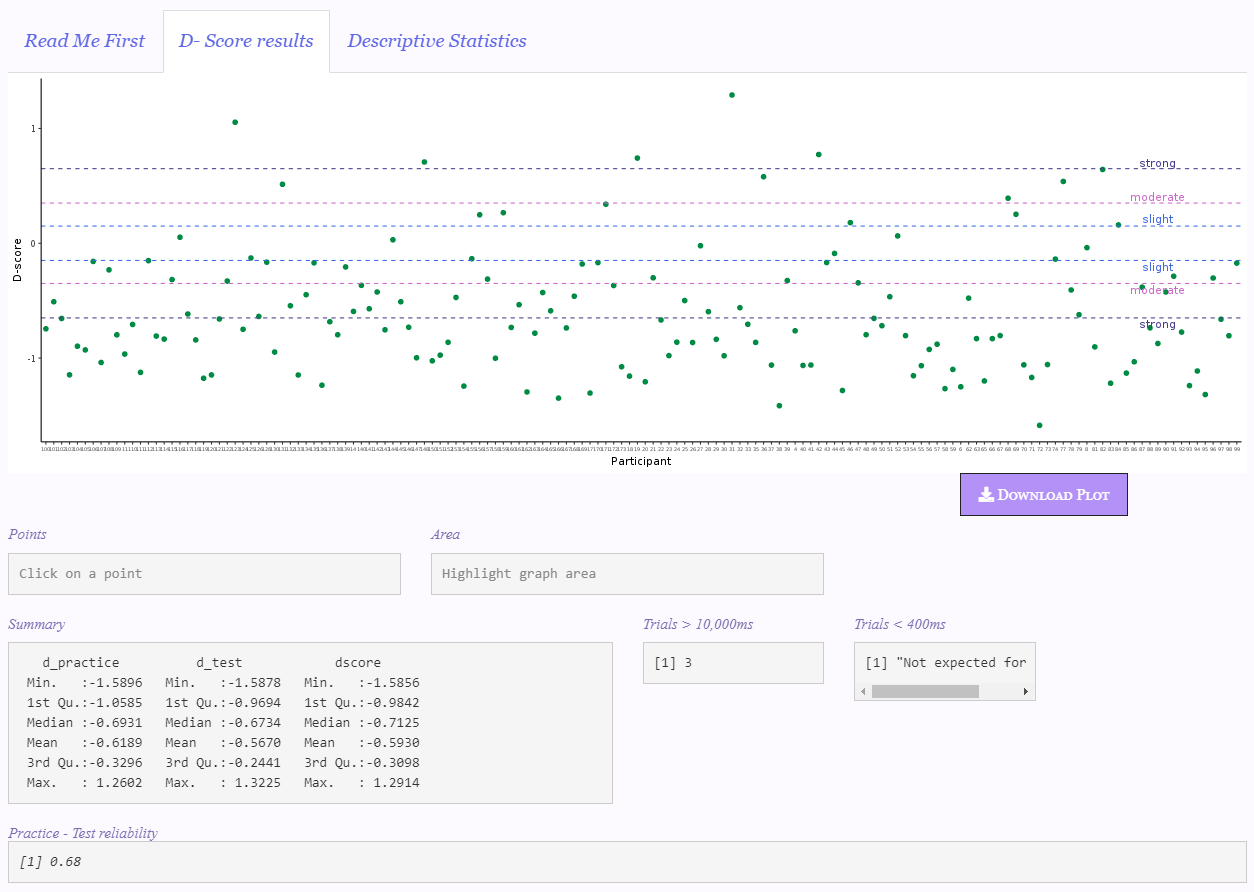
\includegraphics[width=\linewidth]{resultsApp.png}
	\caption{DscoreApp results panel.}
	\label{fig:dscoreapp}
\end{figure}
%
Both descriptive statistics of the results and their graphical representation are available at the same time, and they change interactively as users change the configuration in the ``Input'' panel. 
The \texttt{Summary} box reports the descriptive statistics of the $D_{\text{practice}}$, $D_{\text{test}}$, and the actual \emph{D} score. 
The \texttt{Trials > 10,000ms} box reports the number of trials discarded because of a slow latency (if any), while the \texttt{Trials < 400ms} box reports the number of trials discarded because of fast response times. This box is populated only when a \emph{D} score with fast trials deletion is selected, otherwise the ``Not expected for this \emph{D}'' label is displayed. 
The \texttt{Practice-Test reliability} box contains the IAT reliability computed as the correlation between associative practice and associative test blocks across participants \cite<see>[for further details]{gaw2017}.

Graphical representation is a convenient way to identify extreme scores or particular response patterns. Since it might be difficult to link a particular point (or points area) in the graph with the corresponding respondent ID in the data set, DscoreApp comes with two handy tools designed to access the IDs of the respondents from the graph. By clicking on a point in the graph, the ID of the participant that corresponds to the selected point, and his/her \emph{D} score, appears in the \texttt{Points} box. 
By highlighting an area of the graph, the IDs of participants included in the area, along with their \emph{D} scores appears in  the \texttt{Area} box.
The \texttt{Points} and \texttt{Area} boxes are represented in Figure \ref{fig:dscoreapp}, right underneath the graphical representation of the results.

DscoreApp provides users with different options for the graphical representation of the results (Figure \ref{fig:dscoregraph}), at both the individual (Figure \ref{fig:point}) and sample (Figure \ref{fig:hist}, \ref{fig:dens}, \ref{fig:histdens}) levels. 
\begin{figure}[h!]
	\centering 
	\begin{subfigure}{0.45\linewidth}
		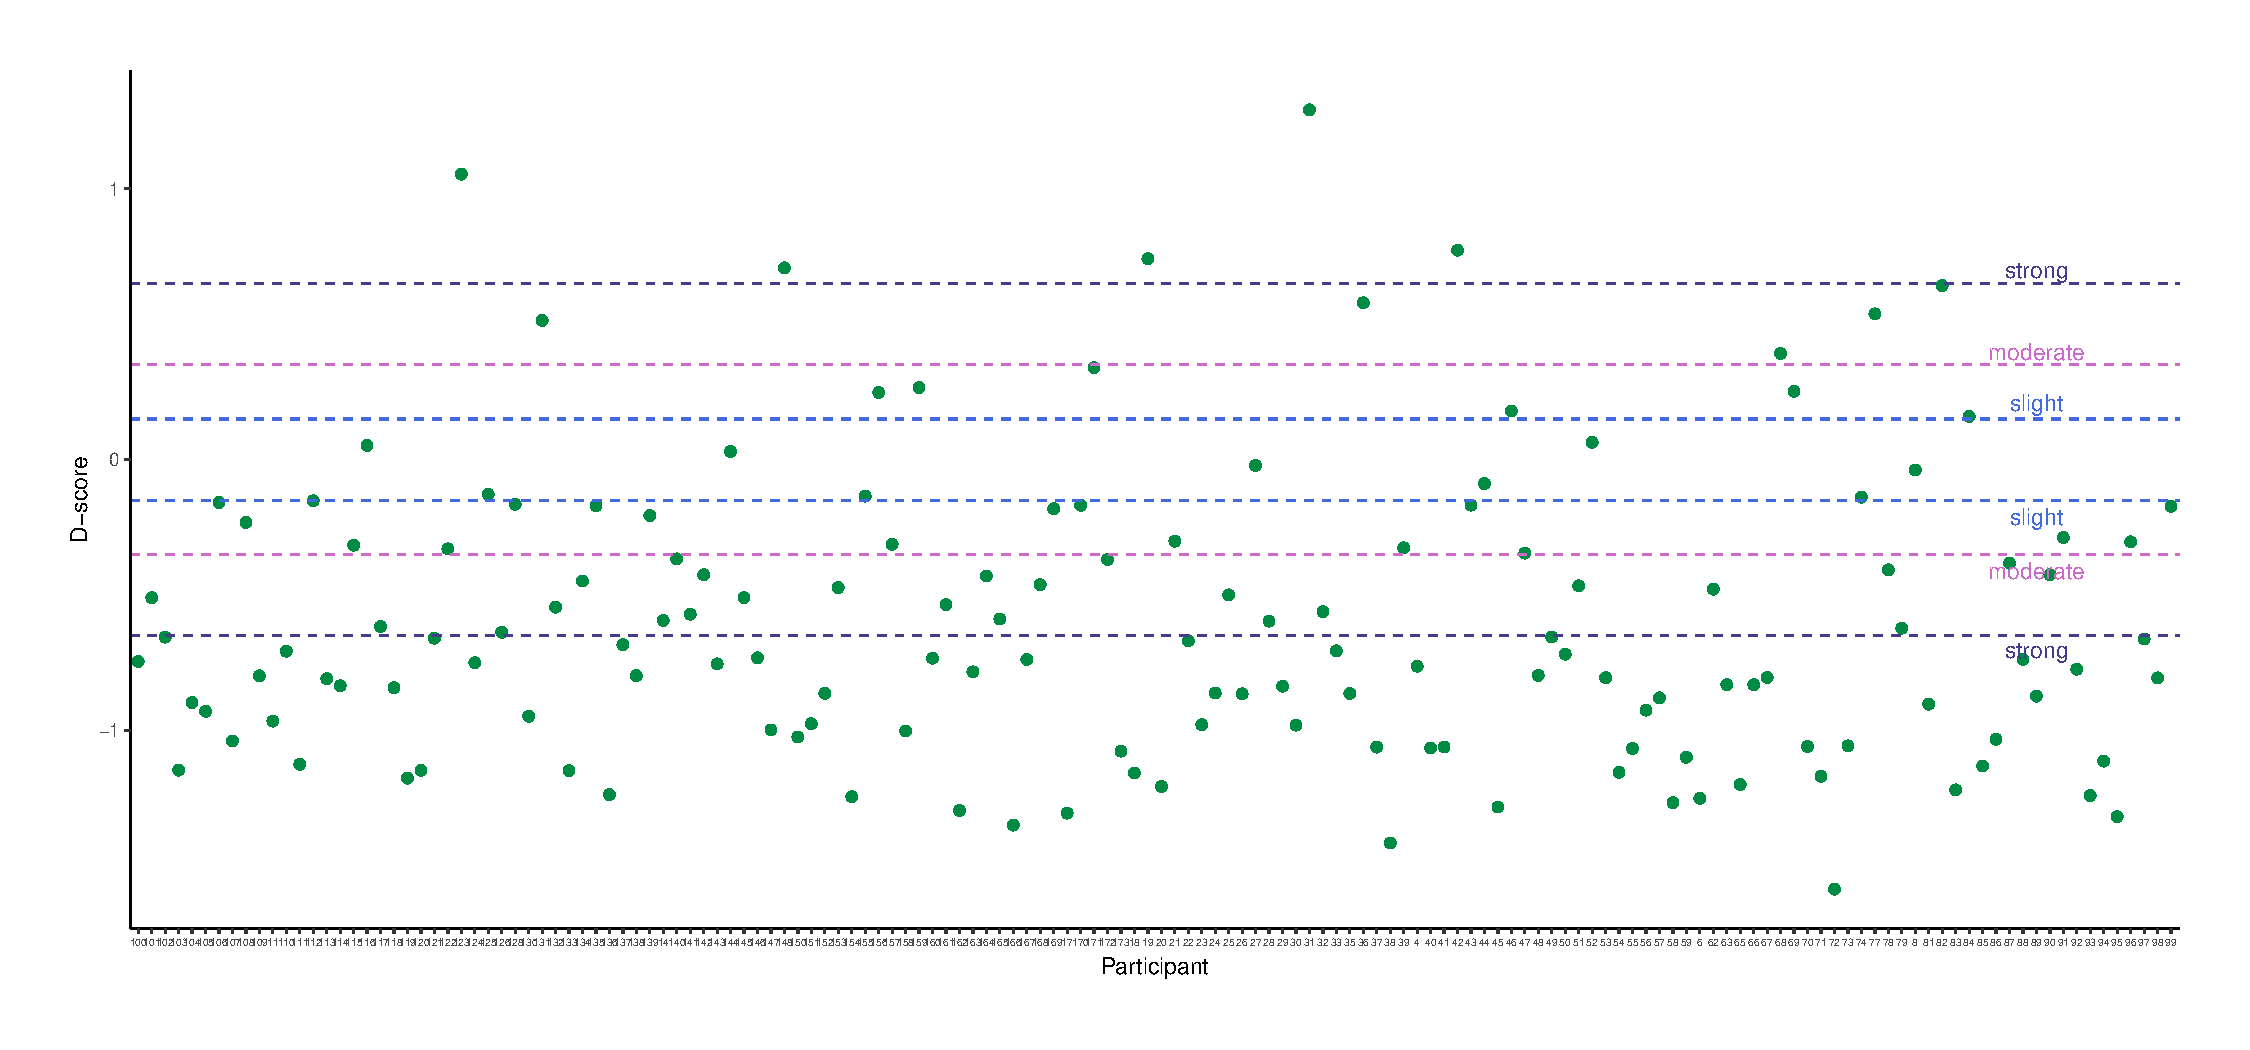
\includegraphics[width=\linewidth]{PointDefaultDscore3.pdf}
		\caption{Points graph.}
		\label{fig:point}
	\end{subfigure}
	\begin{subfigure}{0.45\linewidth}
		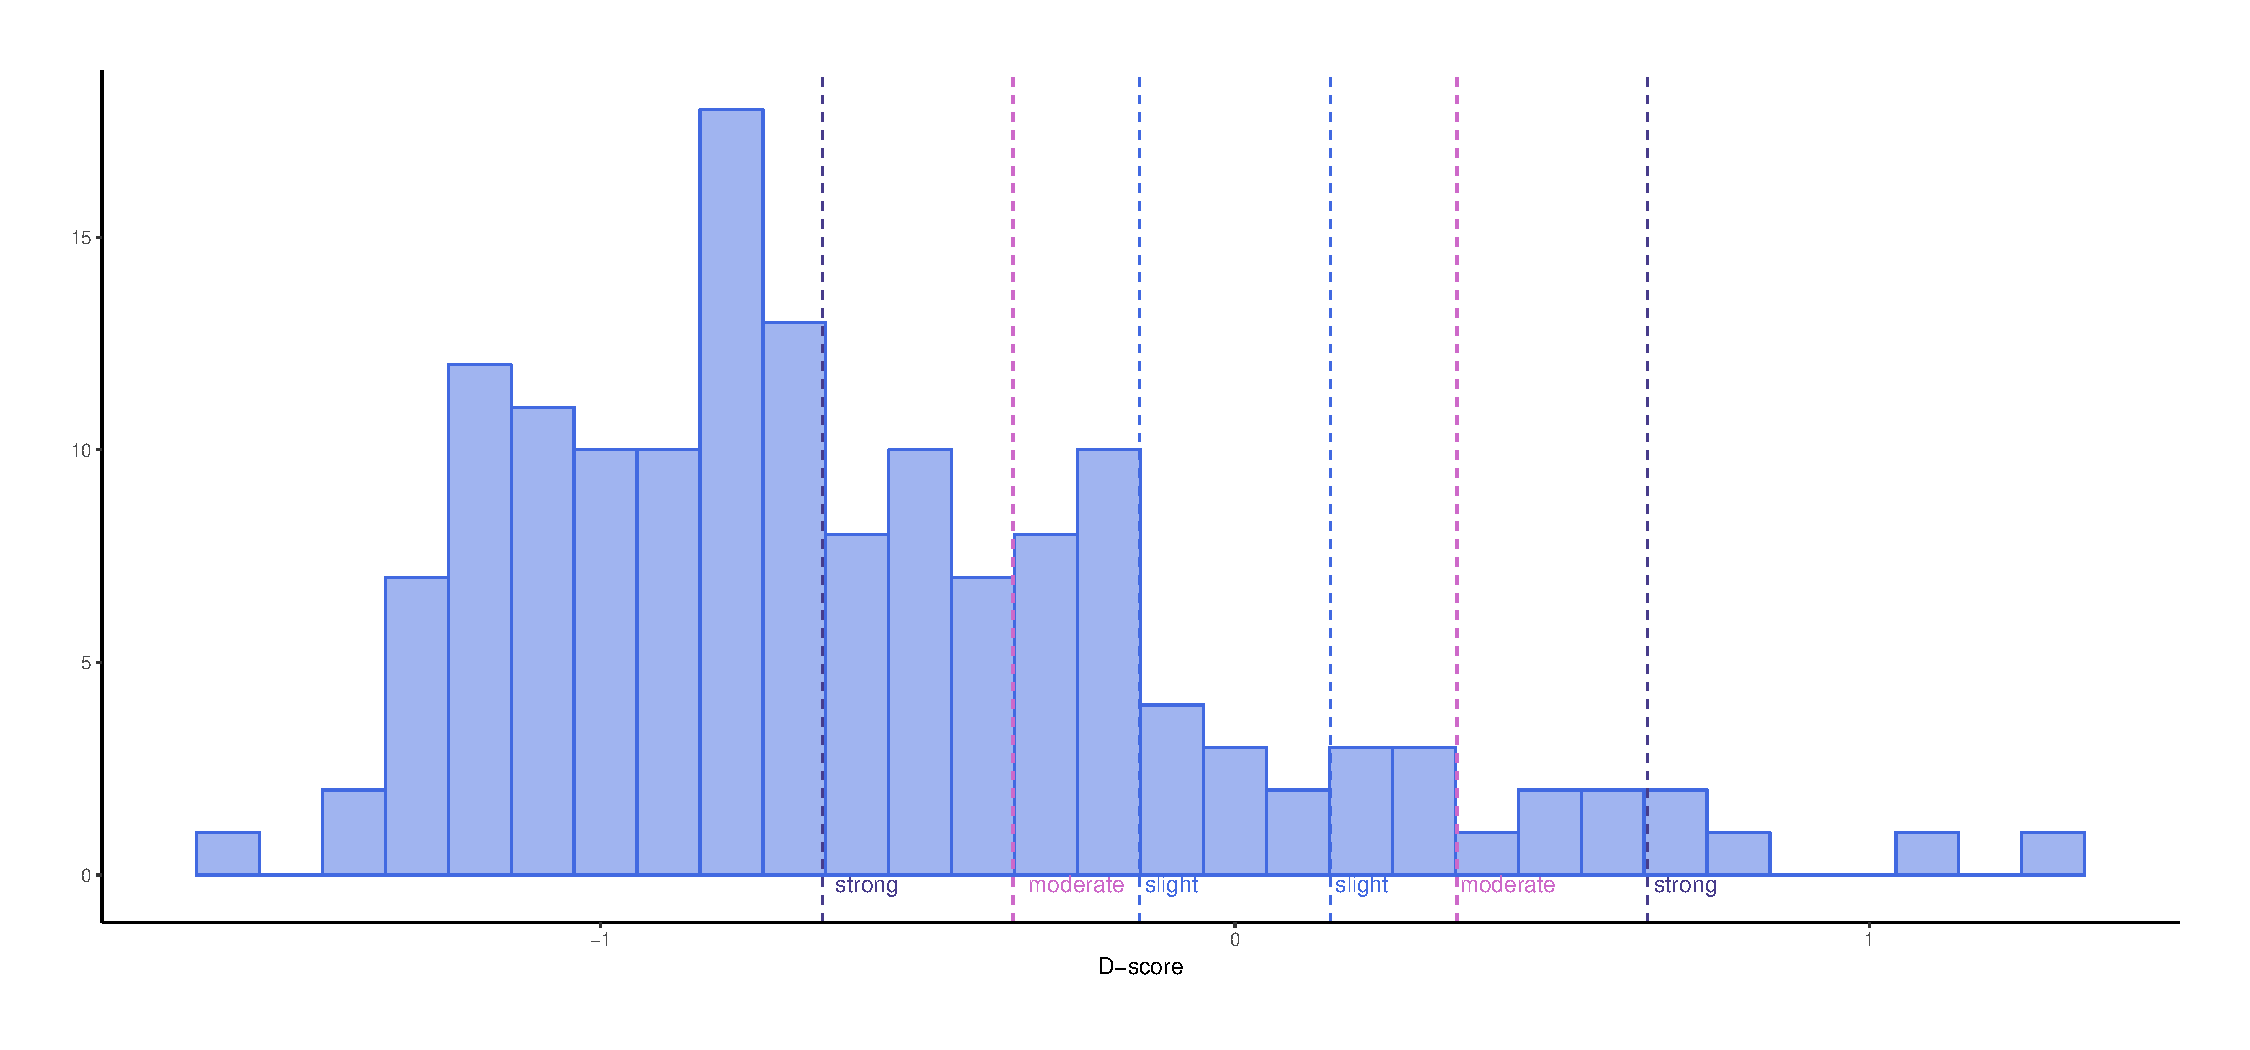
\includegraphics[width=\linewidth]{HistogramDscore3.pdf}
		\caption{Histogram.}
		\label{fig:hist}
	\end{subfigure}
	\begin{subfigure}{0.45\linewidth}
		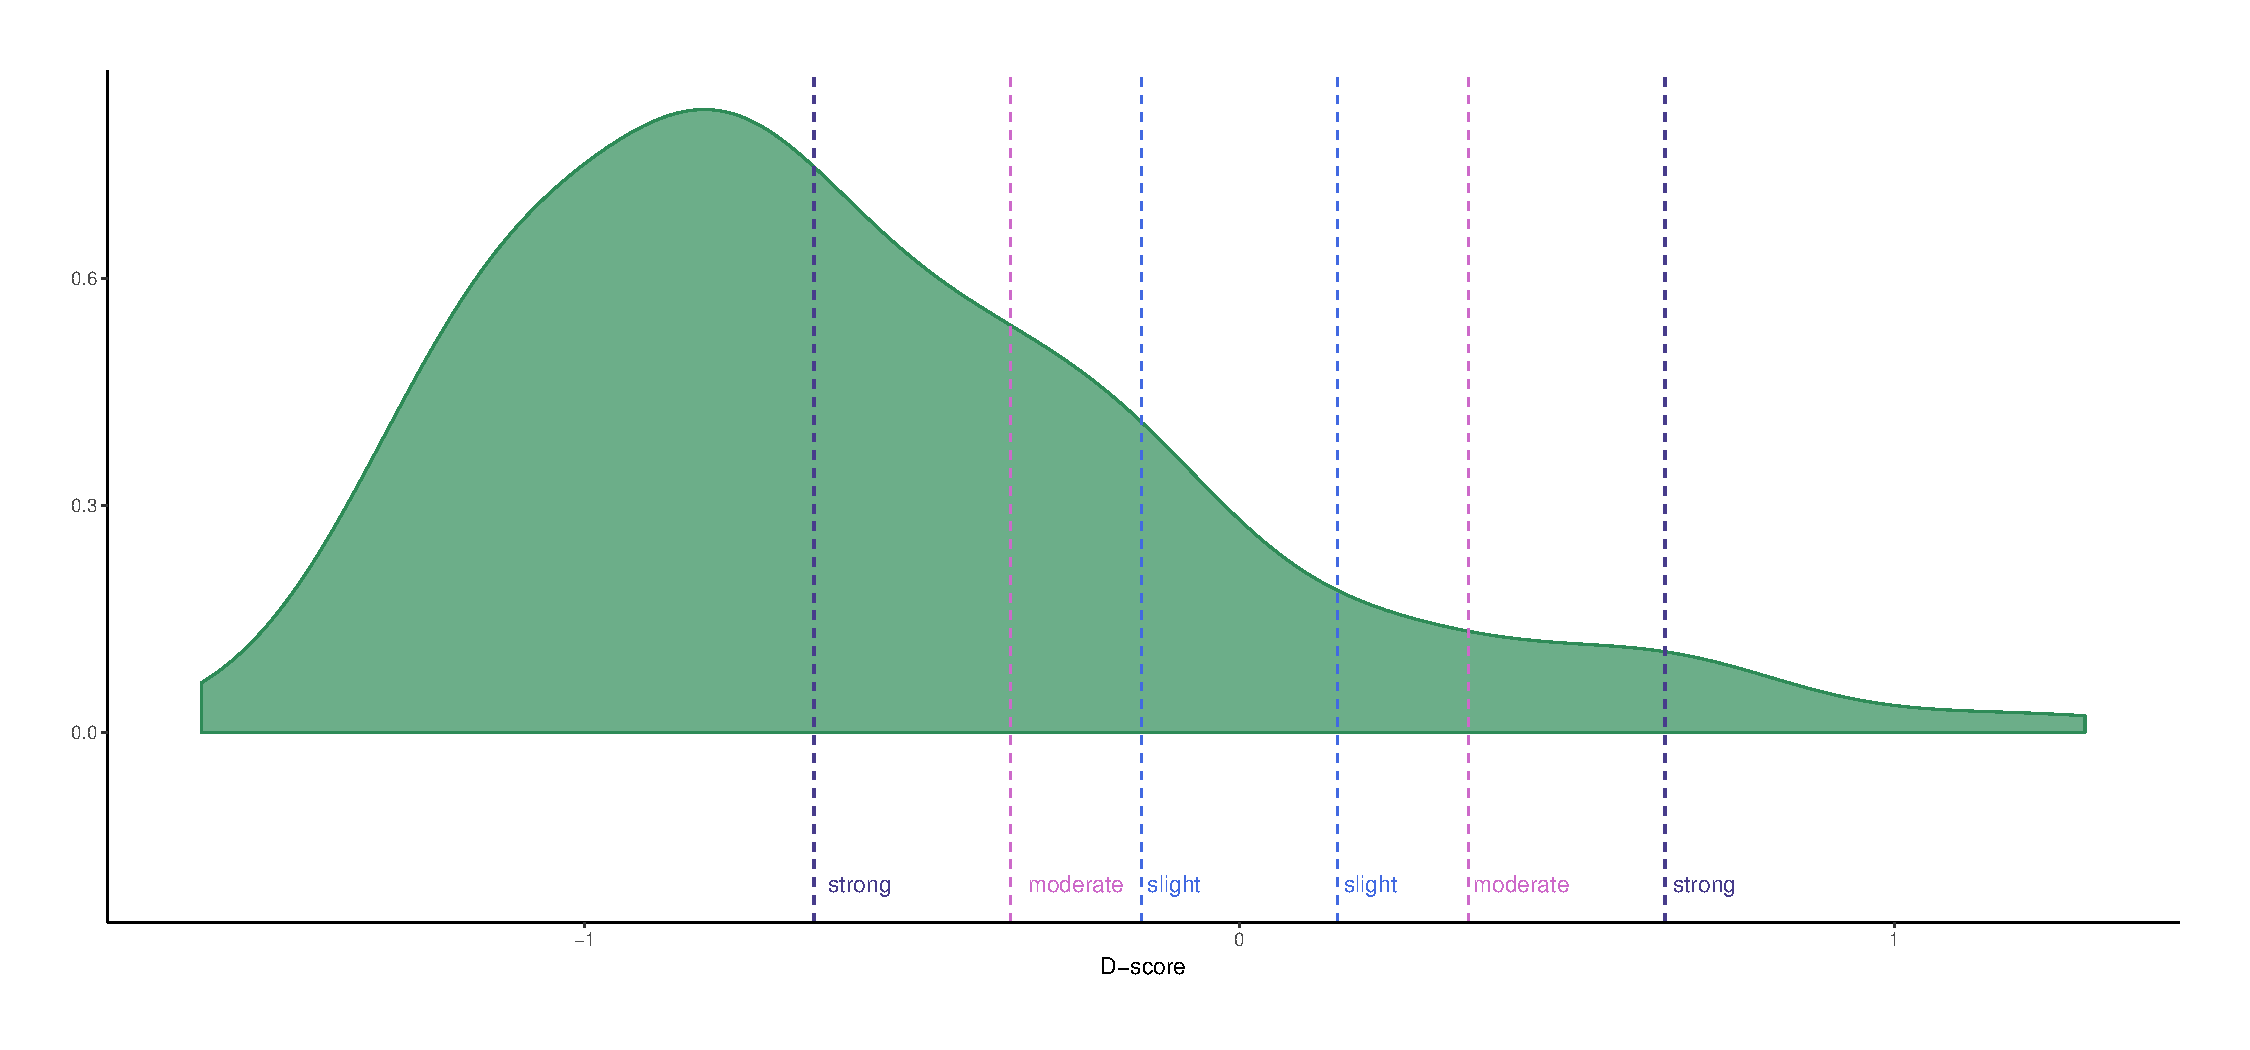
\includegraphics[width=\linewidth]{DensityDscore3.pdf}
		\caption{Density.}
		\label{fig:dens}
	\end{subfigure}
	\begin{subfigure}{0.45\linewidth}
		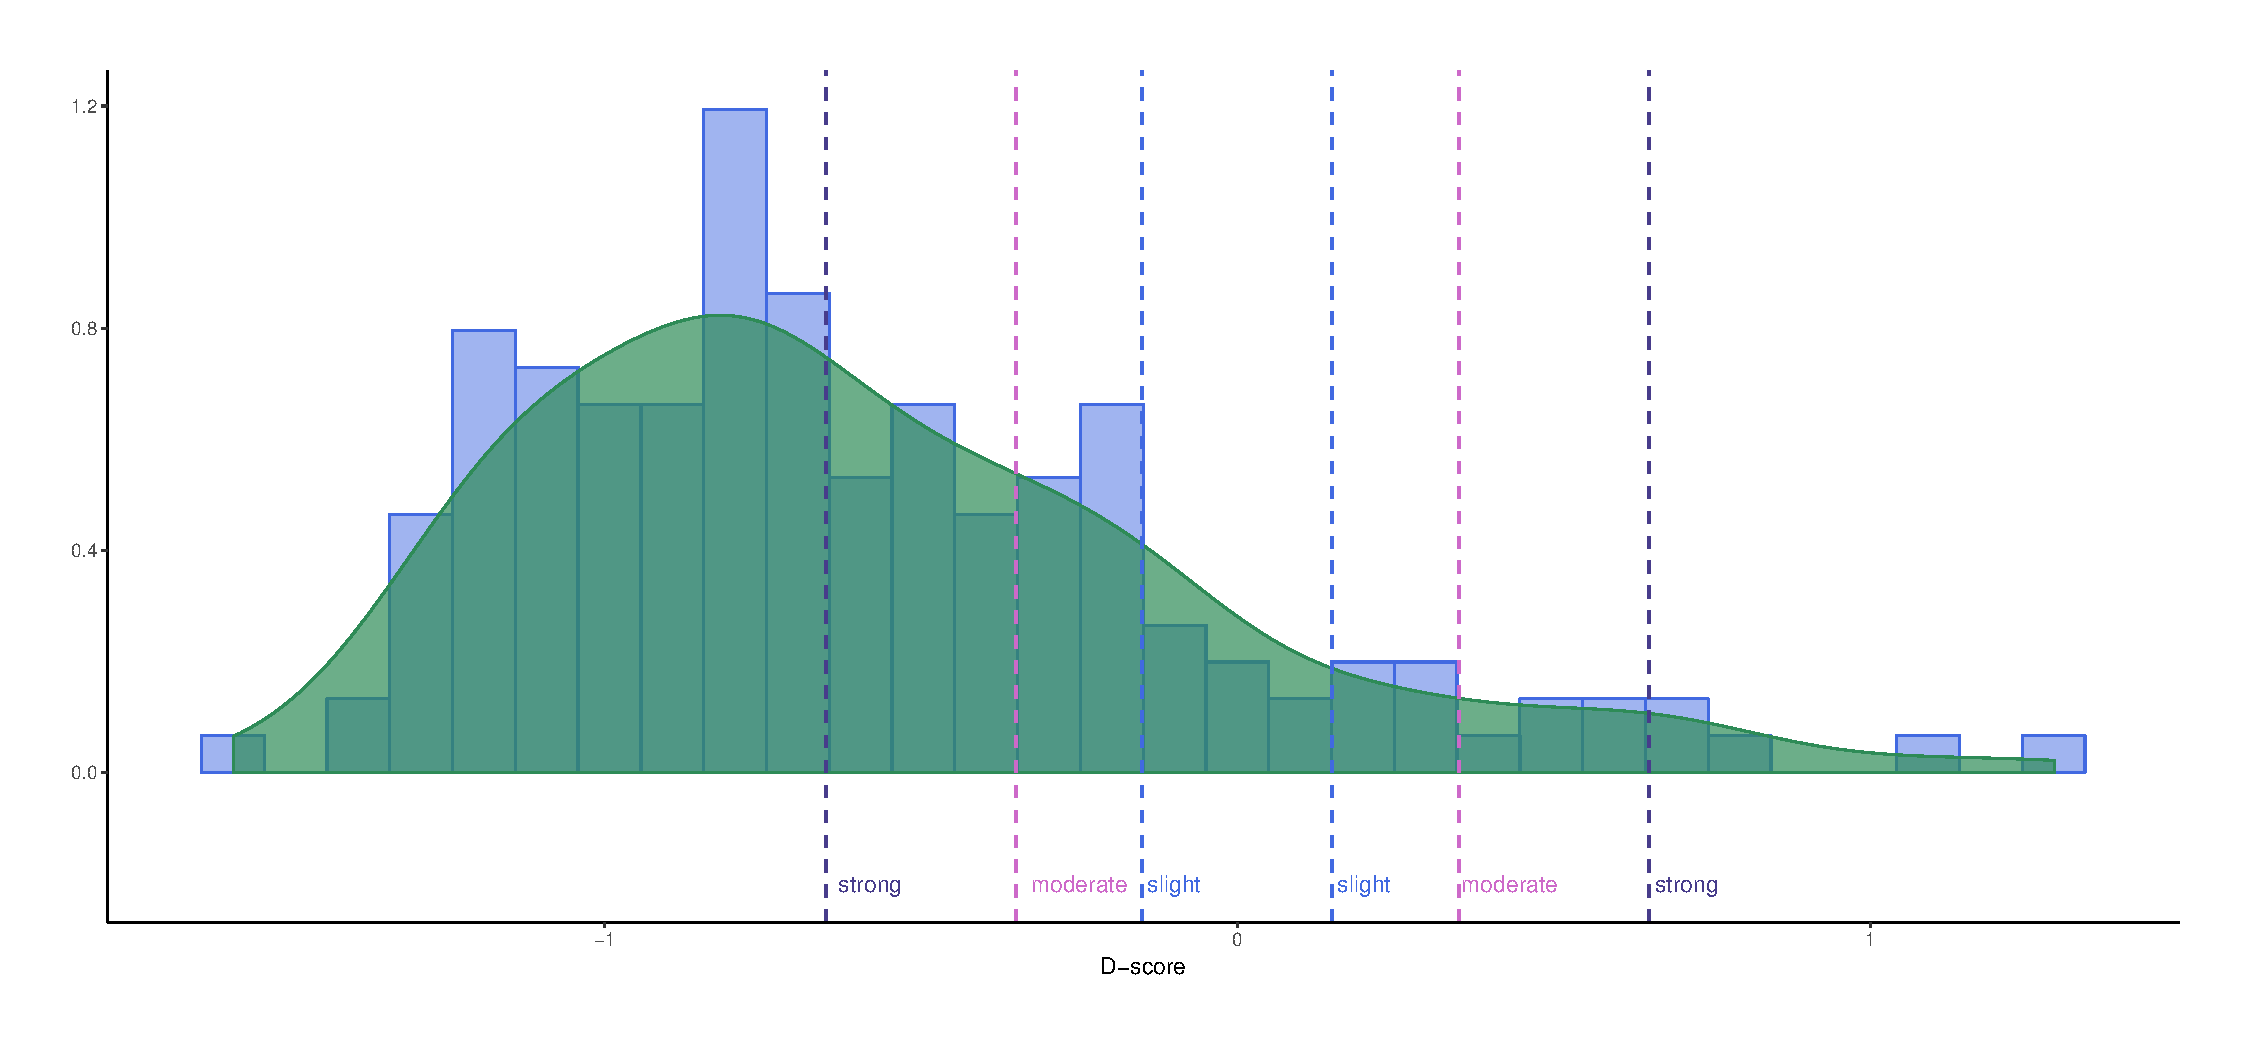
\includegraphics[width=\linewidth]{HistDensDscore3.pdf}
		\caption{Histogram and Density.}
		\label{fig:histdens}
	\end{subfigure}
	\caption{\label{fig:dscoregraph} Available graph representations.}
\end{figure}
All the graphical representations can be downloaded in a .pdf format.

\subsection{The \texttt{implicitMeasures} package}\label{sub:package}

Despite both the IAT and the SC-IAT are commonly used for the implicit assessment of several constructs, \texttt{R} packages for the computation of only the IAT \emph{D} score are available, while there are no packages for computing the SC-IAT \emph{D} score.

Besides the above-mentioned shortcomings of the \verb*|R| packages for computing the IAT \emph{D} score, there are also issues related to the replicability of the results.
The choice on which IAT \emph{D} score algorithm to compute might influence the results and the conclusions that are drawn from them \cite{ellithorpe2015}. Moreover, in many cases researchers fail to report of the exact \emph{D} score algorithm they decided to use \cite{ellithorpe2015}. 
Replicability issues might also rise from mistakes that might be caused by the many steps needed to clean and prepare the starting data set for computing the \emph{D} score \cite{ellithorpe2015}. 

Despite DscoreApp addresses the majority of the replicability issues, it presents some drawbacks as well. Firstly, since the code is into the Shiny interface, it cannot be called from the command line, making  impossible to replicate it and the results obtained with its use. 
To be fair, this is a general and outstanding issue concerning Shiny apps in general. 
This might not be a concern for general users, but it is indeed a problem in an open science framework where every code should be accessible and replicable with no effort at any time.
Moreover, the downloadable graphical representations are provided in a pdf format. As such, they cannot be further modified.

The \verb*|implicitMeasures| package \cite{implicit, implicitMeasures} was aimed at addressing the issues concerning both \verb*|R| packages and DscoreApp. It provides an easy and open source way to clean and score both the IAT and the SC-IAT, to easily compare different algorithms of the  IAT \emph{D} score, and to provide clear and customizable plots. The \verb*|implicitMeasures| package has been published in \citeA{implicitMeasures}.


The source code of \verb*|implicitMeasures| is available on GitHub (\url{https://github.com/OttaviaE/implicitMeasures}). The package is downloadable from CRAN  (\url{https://cran.r-project.org/web/packages/implicitMeasures/index.html}).

Table \ref{tab:implicitmeasures} provides an overview of the functions included in the \verb*|implicitMeasures| package.
\begin{table}[h!]
	\centering \onehalfspacing
	\caption{\label{tab:implicitmeasures} Contents and functions \texttt{implicitMeasures}.}
	\begin{tabular}{p{5cm} p{9cm}}
		\hline
		Function & Description \\
		\hline
		
		\verb*|clean_iat()|& Prepare and clean IAT data\\
		\verb*|clean_sciat()|& Prepare and clean SCIAT data\\
		\verb*|compute_iat()|& Compute IAT \emph{D} score \\
		\verb*|compute_sciat()|& Compute SC-IAT \emph{D} score \\
		\verb*|descript_d()|& Print descriptive table of \emph{D} scores (also in \LaTeX) \\
		\verb*|d_density()|& Plot either IAT or SC-IAT scores (distribution) \\
		\verb*|d_point()|& Plot either IAT or SC-IAT scores (points) \\
		\verb*|IAT_rel()|& Compute IAT reliability \\
		\verb*|multi_dsciat()|& Plot scores resulting from two SC-IATs\\
		\verb*|multi_dscore()|& Compute and plot multiple IAT \emph{D} scores\\
		\verb*|raw_data()|& Example data set \\
		\bottomrule
	\end{tabular}
\end{table}
The \verb*|implicitMeaures| package provides an easy way to compute the algorithms for the both the IAT and the SC-IAT in an automated way. By explicitly referring to the \emph{D} score algorithm that has been used for computing the IAT \emph{D} score, other users can easily replicate the results. 
Additionally, the possibility to compute all available algorithms for the IAT \emph{D} score allows for an easy comparison between them. This makes possible to investigate whether or how the elimination of fast responses or the error replacement strategies affect the results. 

%Indeed, preventing computational mistakes, having a clear reference on the specific \emph{D} score that has been computed, and comparing alternative \emph{D} score algorithms can have a positive influence on the replicability of the results \citeA{ellithorpe2015}.

All objects created with the functions in the \verb*|implicitMeasures| package can be exported in external files. For example, the data frame obtained from the \verb*|clean_iat()| function can be easily exported in a CSV file and then uploaded to DscoreApp (see Section \ref{sec:dscoreapp}).  

The functions for plotting the results are based on \verb*|ggplot2| \cite{ggplot2}, and they can be further modified by users, for instance by taking out the legend, adjusting the figure margins, changing labels and font. All the plots are then exportable as images (.jpg or .png) or as a .pdf.


\chapter{Formal modeling}\label{chap:formalModel}

This chapter provides a brief overview of the formal models introduced for modeling IAT data. 
These models are generally aimed at the investigation of the cognitive processes and the automatic associations involved during the performance at the IAT. Their advantages and drawbacks are outlined and discussed.

Some of these models  are solely based on accuracy responses (Section \ref{sec:multimodel}), while others are able to concurrently model accuracy and time responses (Section \ref{sec:timeacc}).
Despite the important and useful information provided at the sample level and/or the stimulus categories level, none of these models provides detailed information on the singular stimulus.

The Rasch modeling of IAT data can overcome this issue, as illustrated in Section \ref{sec:mfrm}. Although this approach provides stimulus-specific information, it also comes with some drawbacks, mostly related to the discretization of the response times and to the overlooking of the fully-crossed structure of the IAT.


\section{Multinomial Models}\label{sec:multimodel}
\subsection{The Quad Model}\label{sub:quad}
The Quad model \cite{Conrey2005} is a multinomial processing tree model introduced for disentangling the contribution of automatic processes from that of controlled processes to the performance of the respondents at the IAT. 
The Quad model is entirely based on accuracy responses, and it exploits the logic of the assumption on which the IAT is based (i.e., response compatibility, according to which responses are faster and more accurate in the condition consistent with one's automatically activated associations). 

According to this model, the observed accuracy responses are determined by the activation (or lack of thereof) of four qualitatively different processes, characterized by different levels of automaticity and controllability.
These processes are the automatic activation of an association triggered by the target stimulus (\emph{activation association}, \emph{AC}), the ability to correctly identify the category to which the stimulus belongs (\emph{discriminability}, \emph{D}), the ability to overcome any automatically activated associations (\emph{overcoming bias}, \emph{OB}), and the influence of any response bias that may intervene in absence of any other process (\emph{guessing}, \emph{G}). A graphical representation of the Quad model is provided in Figure \ref{fig:quad}.
\begin{landscape}
	\pagestyle{plain}
	\begin{figure}
		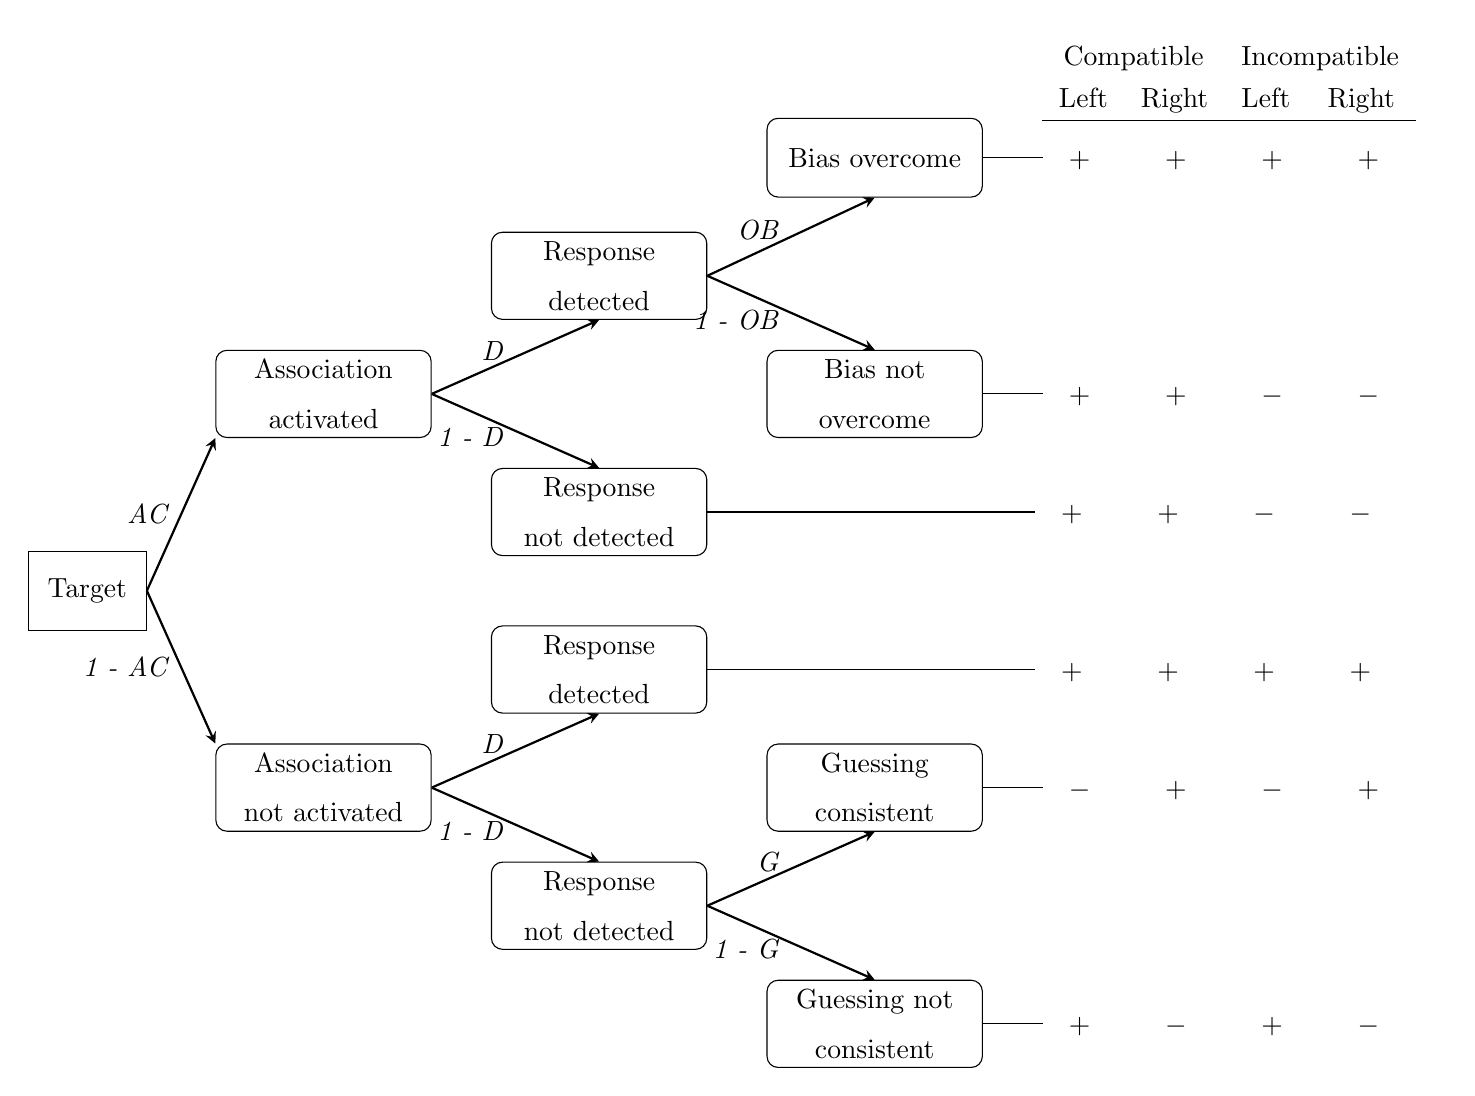
\begin{tikzpicture}[node distance=2cm]
			\node (start) [startstop] {Target};
			\node (ac) [process, right of = start, yshift=2.5cm, xshift = 1cm] {Association activated};
			\node (notac) [process, right of = start, yshift=-2.5cm, xshift = 1cm] {Association not activated};
			\node (d) [process, right of = ac, yshift=1.5cm, xshift = 1.5cm] {Response detected};
			\node (notd) [process, right of = ac, yshift=-1.5cm, xshift = 1.5cm] {Response not detected};
			\node (ob) [process, right of = d, yshift=1.5cm, xshift = 1.5cm] {Bias overcome};
			\node (notob) [process, right of = d, yshift=-1.5cm, xshift = 1.5cm] {Bias not overcome};
			\node (d1) [process, right of = notac, yshift=1.5cm, xshift = 1.5cm] {Response detected};
			\node (notd1) [process, right of = notac, yshift=-1.5cm, xshift = 1.5cm] {Response not detected};
			\node (g) [process, right of = notd1, yshift=1.5cm, xshift = 1.5cm] {Guessing consistent};
			\node (notg) [process, right of = notd1, yshift=-1.5cm, xshift = 1.5cm] {Guessing not consistent};
			\path [arrow] (start.east) edge node[anchor=east] {\emph{AC}} (ac.south west);
			\path [arrow] (start.east) edge node[anchor=east] {\emph{1 - AC}} (notac.north west);
			\path [arrow] (ac.east) edge node[anchor=east, yshift = 0.08cm] {\emph{D}} (d.south);
			\path [arrow] (ac.east) edge node[anchor=east, yshift = -0.08cm] {\emph{1 - D}} (notd.north);
			\path [arrow] (d.east) edge node[anchor=east, yshift = 0.08cm] {\emph{OB}} (ob.south);
			\path [arrow] (d.east) edge node[anchor=east, yshift = -0.09cm] {\emph{1 - OB}} (notob.north);
			\path [arrow] (notac.east) edge node[anchor=east, yshift = 0.08cm] {\emph{D}} (d1.south);
			\path [arrow] (notac.east) edge node[anchor=east, yshift = -0.08cm] {\emph{1 - D}} (notd1.north);
			\path [arrow] (notd1.east) edge node[anchor=east, yshift=0.08cm] {\emph{G}} (g.south);
			\path [arrow] (notd1.east) edge node[anchor=east, yshift = -0.08cm] {\emph{1 - G}} (notg.north);
			
			\node (table) [rectangle ,right of = ob, xshift = 2.5cm, yshift = 1cm]{%
				\onehalfspacing
				\begin{tabular}{c c c c}
					\multicolumn{2}{c}{Compatible} & \multicolumn{2}{c}{Incompatible}\\
					
					\multicolumn{1}{c}{Left} & \multicolumn{1}{c}{Right} & \multicolumn{1}{c}{Left} & \multicolumn{1}{c}{Right} \\
					\hline
				\end{tabular}
			};
			\node (first) [rectangle ,right of = ob, xshift = 2.7cm] {%
				\begin{tabular}{p{0.8cm} p{0.8cm} p{0.8cm} p{0.8cm}}
					$+$ & $+$ & $+$ & $+$ \\
			\end{tabular}};
			\node (second) [rectangle ,right of = notob, xshift = 2.7cm] {%
				\begin{tabular}{p{0.8cm} p{0.8cm} p{0.8cm} p{0.8cm}}
					$+$ & $+$ & $-$ & $-$ \\
			\end{tabular}};
			\node (third) [rectangle ,right of = notd, xshift = 6.1cm] {%
				\begin{tabular}{p{0.8cm} p{0.8cm} p{0.8cm} p{0.8cm}}
					$+$ & $+$ & $-$ & $-$ \\
			\end{tabular}};
			\node (fourth) [rectangle ,right of = d1, xshift = 6.1cm] {%
				\begin{tabular}{p{0.8cm} p{0.8cm} p{0.8cm} p{0.8cm}}
					$+$ & $+$ & $+$ & $+$ \\
			\end{tabular}};
			\node (fifth) [rectangle ,right of = g, xshift = 2.7cm] {%
				\begin{tabular}{p{0.8cm} p{0.8cm} p{0.8cm} p{0.8cm}}
					$-$ & $+$ & $-$ & $+$ \\
			\end{tabular}};
			\node (sixth) [rectangle ,right of = notg, xshift = 2.7cm] {%
				\begin{tabular}{p{0.8cm} p{0.8cm} p{0.8cm} p{0.8cm}}
					$+$ & $-$ & $+$ & $-$ \\
			\end{tabular}};
			\path [-] (ob.east) edge (first.west);
			\path [-] (notob.east) edge (second.west);
			\path [-] (notd.east) edge (third.west);
			\path [-] (d1.east) edge (fourth.west);
			\path [-] (g.east) edge (fifth.west);
			\path [-] (notg.east) edge (sixth.west);
		\end{tikzpicture}
		\caption{\label{fig:quad} Quad Model \protect\cite<adapted from>{Conrey2005}. Parameters with arrows pointing towards them are conditional on all the preceding ones. $+$: correct response (stimulus assigned to the correct category), $-$: incorrect response (stimulus assigned to the incorrect category).}
	\end{figure}
\end{landscape}
Each path in Figure \ref{fig:quad} represents the likelihood that a parameter is activated. The activation of the parameters are conditional on the activation of the parameters preceding them. 

The \emph{AC} parameter describes the probability that an automatic association is activated by the triggering stimulus. This parameter expresses the most automatic component of the model and it is directly related to the strength of the association activated by the stimulus. The stronger the association between the stimulus and a negative/positive attribute, the more likely the activation of the automatic association.

The probability of giving the correct response does not solely depend on the activation of the automatic association, but also on the ability to identify the correct response among the available ones. In turn, this ability depends on the availability of cognitive resources and on the application of some effort in determining the correct response. The \emph{D} parameter represents the likelihood that the correct response \emph{can} be identified, not the likelihood that the correct response \emph{is} identified. The \emph{D} parameter depends on several factors, including the motivation to have a good performance, the attention paid to the stimulus, and the availability of relevant information in memory.

If a negative automatic association is activated by the triggering stimulus, the respondent might try to fake the response in a socially desirable way. The \emph{OB} parameter represents the likelihood that an activated bias is overcome in favor of a deliberate, and probably more desirable, response. 

The processes described by the \emph{D} and \emph{OB} parameters are the ones that are mostly influenced by motivation and that mostly depend on the availability of cognitive resources  to be activated and drive the correct response. They reflect two different aspects of controlled processes. The controlled process involved by the \emph{D} parameter is an active search for the correct response, while the process described by the \emph{OB} parameter  exploits control for the inhibition of the response activated by the automatic association. 

If none of the above-mentioned processes is activated, then the responses can be influenced by a response bias, such as the tendency to respond with the left response key. The \emph{G} parameter represents the likelihood that a response bias, different than the automatic association, is activated and drives the responses. 

As previously mentioned, the parameters of the Quad model are estimated from the observed proportions of a correct response given a stimulus type. Each arrow moving from left to right in Figure \ref{fig:quad} represents the multiplication between the independent probabilities of each process. It results in the prediction of a specific response, either correct or incorrect. 
The sum of all probabilities associated to that response is the total probability of that response.

Consider a respondent with an implicit preference for Pepsi over Coke. For him/her, the incompatible condition is the Coke/Good-Pepsi/Bad condition. The probability that this respondent has of correctly sorting a can of Coke in the incompatible condition is given by the sum of the paths resulting in a correct response. In this case, three processes lead to the correct response. As such, the resulting equation is: $\text{P(correct}|\text{Coke, incompatible)} = AC \times D \times OB + (1-AC)\times D + (1-AC)\times (1-D) \times (1-G)$. 
The first path ($AC \times D \times OB$) represents the probability that an automatic association is activated by the stimulus ($AC$), that the response can be identified ($D$), and that the bias is successfully overcome ($OB$).
The second path  ($(1-AC)\times D$) represents the probability that the automatic association is not activated ($1 - AC$) and that the response can be identified ($D$). 
Finally, the third path ($(1-AC)\times (1-D) \times (1-G)$) represents the probability that the association is not activated ($1-AC$), the correct response cannot be detected ($1-D$), and that automatically responding with the left response key is not an effect of guessing ($1-G$).
The sum of the products of the independent probabilities yielded by each path results in the total probability of a correct response to the stimulus.


By qualitatively disentangling the nature of the processes intervening during the performance at the IAT, the Quad model offers detailed information on the IAT functioning. 
Most importantly, the Quad model explicitly points out that the performance at the IAT should not be taken as the sole expression of automatic processes. Rather, the contribution of controlled processes should be acknowledged and taken into account for the explanation of social phenomena. 

This point has crucial repercussion on applied researches using the IAT.
For instance, in an IAT for the assessment of implicit prejudice, it would be of the uttermost importance to understand whether a resulting negative \emph{D} score (e.g., a \emph{D} score indicating a preference for White people over Black people) is actually due to the automatic activation of the association between one of the targeted groups and negative attributes or to other, more controlled, processes, such as the inability to identify the correct response.  
The information provided by the \emph{OB} parameter allows for understanding whether a positive \emph{D} score is the expression of genuinely automatic associations between the stigmatized group and positive attributes or by the desire to conceal negative attitudes towards the stigmatized group.
Both the \emph{AC} and \emph{OB} parameters are associated with the typical IAT \emph{D} score \cite{Conrey2005}.
The \emph{D} score was found to be positively associated with the \emph{AC} parameter (i.e., the stronger the association activated by the stimulus, the higher the \emph{D} score value). 
Moreover, the \emph{AC} parameter allowed for pinpointing the contribution of distinct associations in a Race IAT, according to which both White-pleasant automatic associations and Black-unpleasant ones were related with the \emph{D} score. The \emph{D} score is hence capturing two distinct associations, and it is confounding them into a unique score. 
The \emph{D} score was negatively associated to the ability of suppressing an automatic activated association described by the \emph{OB} parameter. The higher the ability to overcome the bias, and hence the value of \emph{OB}, the lower the IAT effect as expressed by the \emph{D} score.

This evidence suggests that the \emph{D} score confounds different information into a single generic score. Firstly, it is not possible to ascertain which of the specific automatic associations drives the performance at the IAT, leaving its meaning partially obscure. 
Moreover, controlled and automatic processes cannot be distinguished from one another, and their unique contribution is lost. It is not possible to ascertain whether the performance is driven by an actual automatic association or if the IAT effect reflects the ability of the respondents to detect the correct response or their ability of overcoming an automatic activated bias. 
It appears evident that distinguishing between these processes is extremely important when inferences on sensitive psychological constructs, such as implicit bias, are made. Indeed, the implications of saying that a sample of individuals is implicitly biased towards a social group are extremely different from saying that the sample has a high ability in detecting the correct responses.
The \emph{D} score alone cannot be used as a measure of pure implicit bias.

The information provided by the Quad model are extremely useful and meaningful for a correct interpretation of the IAT effect. 
However, it should be taken with caution for at least two reasons: The results are entirely based on accuracy responses and the person estimates are at the sample level and not at the individual respondent's level.

Regarding the first issue, the IAT is known to be an easy task -- it is actually designed to be an easy task by choosing highly representative and easy-to-sort stimuli. As such, the error rates are extremely low, unless the respondent was distracted or the task itself did not work properly. This raises issues concerning the estimation of the model parameters and their reliability. Moreover, not using the time responses implies losing the majority of the information that can be retrieved from the IAT data, which can in turn lead to an incorrect interpretation of the results. 
For instance, the higher accuracy of the responses when the automatic associations is activated might be also associated to slower response times \cite<speed-accuracy trade-off,>{Klauer2007}. By considering only the accuracy responses, the Quad model is not able to rule out this possibility, and the conclusions based on the Quad model might be misleading.
%Despite interesting, this result should be taken with caution. Indeed, the Quad model, and the estimation of its parameters, is solely based on the accuracy responses. There are reasons to believe that higher accuracy of the responses when an automatic bias is activated might be associated to slower response times (speed-accuracy trade-off). The Quad model is not able to rule out this possibility, hence the conclusions based on this result might be misleading. 
The \emph{OB} parameter describes the process that controls the accuracy of the responses when an automatic association is activated and, as such, it should be the one mostly affected by the speed-accuracy trade-off. Indeed, results of Study 2 in \citeA{Conrey2005} actually pointed in this direction. The \emph{OB} parameter dropped significantly (i.e., respondents with automatically activated associations were not able to provide the correct response) when a time constraint for giving the response was introduced.
This result does indicate that the \emph{OB} parameter captures a controlled process that needs time to be activated and successfully used. 
Not considering response times for interpreting the results from the \emph{OB} parameter appears to be a fallacy leading to misleading inferences.

Regarding the second issue, the estimates provided by the Quad model are at either the sample level or the stimulus categories level. 
Consequently, both the between--respondents variability and the between--stimuli one are completely ignored. 
Moreover, having estimates at the sample level for the respondents does not allow for investigating their individual differences, which is usually the main objective of applied social psychology. 
Similarly, the information at the level of the singular stimulus is neglected. 

To be fair, in Study 4 in \citeA{Conrey2005} respondent--specific estimates were obtained. 
However, obtaining respondent--specific estimates with the Quad model is tricky given the high error rate needed in the starting contingency table, where stimulus categories are crossed with the associative conditions, within each respondent. To ensure an high error rate value for each possible combination, a longer IAT procedure should be adopted. As such, the Quad model is not feasible for investigating individual differences using IATs of typical length.
%Finally, the estimates provided by the Quad model are either the sample or stimuli category level. Respondent--specific estimates can be obtained as well \cite<e.g., Study 4,>{Conrey2005}, but still the information that can be retrieved from each individual stimulus is not considered.



%According to the Quad Model, the accuracy performance at the IAT depends on four qualitatively distinct processes: (i) the automatic activation of an association triggered by a stimulus, (ii) the ability to discriminate the correct category to which the stimulus belongs, (iii) the ability to overcome automatically activated associations, and (iv) any response bias (e.g., the tendency to respond with the right response key) that may drive the response in absence of any other process. 



\subsection{The ReAL Model}\label{sub:real}

The ReAL model \cite{Meissner2013} is a multinomial processing tree model based on accuracy responses. 
This model is aimed at mathematically distinguishing the contribution of the automatic associations from that of recoding or simplification strategies that might intervene during the performance at the IAT. 

The ReAL model is based on two main assumptions. 
%ReAL model postulates that a part of respondents' performance during the IAT is ascribable to strategies implemented to simplify the categorization task,
The first assumption is that only attitude objects activate automatic evaluative associations. Consequently, evaluative associations influence responding only for attitudes stimuli, while the same does not hold for attributes stimuli. Consequently, attitude objects can be sorted according to their evaluative value, while evaluative attributes cannot be sorted according to the attitude objects to which they are associated.
The second assumption logically follows from the first one. To be recoded into a unique category target stimuli and evaluative attributes must be sharing a common feature, that is, an intrinsic positive or negative value, which is determined by the attitude based associations.
Attitude based associations can facilitate the correct sorting of the target stimuli in the condition consistent with individual's automatically activated association (i.e., compatible) but not in that against individual's  automatically activated association (i.e., incompatible). Therefore, the recoding of target stimuli according to their evaluative dimension facilitates the performance only in the compatible condition, while it hinders it in the incompatible one.
% Consequently, recoding strategies can positively affect the responding only in the condition where the intrinsic value of the objects and the evaluative attributes are consistent between each other.

For example, in the Coke-Good/Pepsi-Bad condition of a Coke-Pepsi IAT, a respondent with a strong preference for Coke might simplify the task by sorting Coke exemplars according to their positive value. 
As such, the task is reduced from a 4-choice task (i.e., \emph{Coke} and \emph{Good}, \emph{Pepsi} and \emph{Bad}) to a 2-choice task (i.e., \emph{Good}, which also includes \emph{Coke}, and everything else). However, this strategy can work only in the associative condition that is consistent with the automatically activated associations of the respondents.

These assumptions allow for assuming that the correct and incorrect response patterns at the IAT are driven by three processes. Their influence on the performance changes according to the specific IAT associative condition, as illustrated in Figure \ref{fig:real}. The illustration of the ReAL model is based on the Coke-Pepsi IAT example introduced in Chapter \ref{chap:intro}, considering a respondent with a strong preference for Coke over Pepsi.

\begin{landscape}
	\thispagestyle{plain}
	\begin{figure}
		\begin{subfigure}{\linewidth}
			\begin{tikzpicture}
				\node[rotate=90, left of = start, yshift=3cm, xshift=1cm] {\large{Compatible condition}};
				\node (start) [startstop] {Target};
				\node (re) [process, right of = start, yshift=1.5cm, xshift = 2cm] {Recoding drives};
				\node (notre) [process, right of = start, yshift=-1.5cm, xshift = 2cm] {Recoding does not drive};
				\node (l) [process, right of = notre, yshift=1.5cm, xshift = 2cm] {Label based};
				\node (notl) [process, right of = notre, yshift=-1.5cm, xshift = 2cm] {Not label based};
				\node (good) [process, right of = notl, yshift=1.5cm, xshift = 2cm] {\emph{Good} automatic associations};
				\node (bad) [process, right of = notl, yshift=-1.5cm, xshift = 2cm] {\emph{Bad} automatic associations};
				\path [arrow] (start.east) edge node[anchor=east, yshift = 0.08cm] {\emph{Re}} (re.south);
				\path [arrow] (start.east) edge node[anchor=east, yshift = -0.08cm] {1-\emph{Re}} (notre.north);
				\path [arrow] (notre.east) edge node[anchor=east, yshift = 0.08cm] {\emph{L}} (l.south);
				\path [arrow] (notre.east) edge node[anchor=east, yshift = -0.08cm] {1-\emph{L}} (notl.north);
				\path [arrow] (notl.east) edge node[anchor=east, yshift = 0.08cm] {\emph{A}} (good.south);
				\path [arrow] (notl.east) edge node[anchor=east, yshift = -0.08cm] {1-\emph{A}} (bad.north);
				
				\node (table) [rectangle ,right of = re, xshift = 10.5cm, yshift = 1.5cm]{%
					\onehalfspacing
					\begin{tabular}{c c}
						\multicolumn{1}{c}{Coke} & \multicolumn{1}{c}{Pepsi}\\
						\hline
					\end{tabular}
				};
				\node (first) [rectangle ,right of = re, xshift = 10.5cm]{%
					\onehalfspacing
					\begin{tabular}{c c}
						$+$ & $+$\\
					\end{tabular}
				};
				\node (second) [rectangle ,right of = l, xshift = 7.5cm]{%
					\onehalfspacing
					\begin{tabular}{c c}
						$+$ & $+$\\
					\end{tabular}
				};
				\node (third) [rectangle ,right of = good, xshift = 4.5cm]{%
					\onehalfspacing
					\begin{tabular}{c c}
						$+$ & $-$\\
					\end{tabular}
				};
				\node (fourth) [rectangle ,right of = bad, xshift = 4.5cm]{%
					\onehalfspacing
					\begin{tabular}{c c}
						$-$ & $+$\\
					\end{tabular}
				};			
				\path [-] (re.east) edge (first.west);
				\path [-] (l.east) edge (second.west);
				\path [-] (good.east) edge (third.west);
				\path [-] (bad.east) edge (fourth.west);
			\end{tikzpicture}
			%\caption{\label{subfig:realcomp} Compatible block.}
		\end{subfigure}
		\par\bigskip
		\begin{subfigure}{\linewidth}
			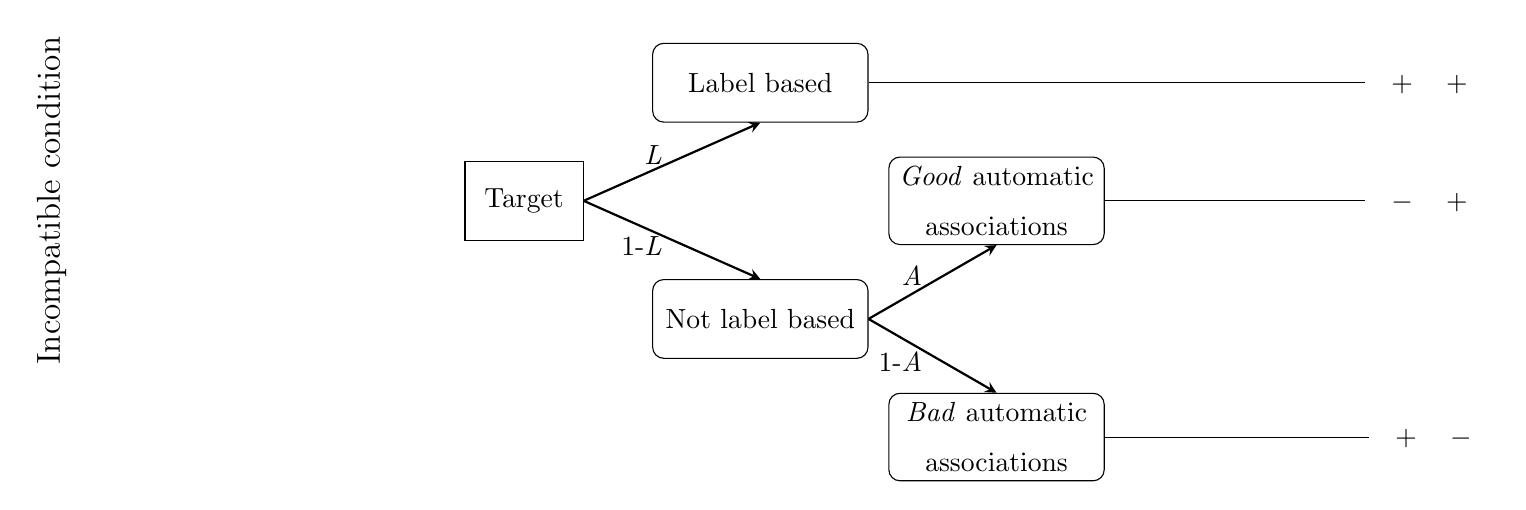
\begin{tikzpicture}
				
				\node (empty) [rectangle] {};
				\node[rotate=90, left of = empty, yshift=3.3cm, xshift=1cm] {\large{Incompatible condition}};
				\node (start) [startstop, right of = empty, xshift = 1.7cm] {Target};
				\node (l) [process, right of = start, yshift=1.5cm, xshift = 2cm] {Label based};
				\node (notl) [process, right of = start, yshift=-1.5cm, xshift = 2cm] {Not label based};
				\node (good) [process, right of = notl, yshift=1.5cm, xshift = 2cm] {\emph{Good} automatic associations};
				\node (bad) [process, right of = notl, yshift=-1.5cm, xshift = 2cm] {\emph{Bad} automatic associations};
				\path [arrow] (start.east) edge node[anchor=east, yshift = 0.08cm] {\emph{L}} (l.south);
				\path [arrow] (start.east) edge node[anchor=east, yshift = -0.08cm] {1-\emph{L}} (notl.north);
				\path [arrow] (notl.east) edge node[anchor=east, yshift = 0.08cm] {\emph{A}} (good.south);
				\path [arrow] (notl.east) edge node[anchor=east, yshift = -0.08cm] {1-\emph{A}} (bad.north);
				
				\node (first) [rectangle ,right of = l, xshift = 7.5cm]{%
					\onehalfspacing
					\begin{tabular}{c c}
						$+$ & $+$\\
					\end{tabular}
				};
				\node (second) [rectangle ,right of = good, xshift = 4.5cm]{%
					\onehalfspacing
					\begin{tabular}{c c}
						$-$ & $+$\\
					\end{tabular}
				};
				\node (third) [rectangle ,right of = bad, xshift = 4.55cm]{%
					\onehalfspacing
					\begin{tabular}{c c}
						$+$ & $-$\\
					\end{tabular}
				};	
				\path [-] (l.east) edge (first.west);
				\path [-] (good.east) edge (second.west);
				\path [-] (bad.east) edge (third.west);	
			\end{tikzpicture}
			%\caption{\label{subfig:realinc}Incompatible Block}
		\end{subfigure}
		\caption{\label{fig:real} ReAL model \protect\cite<adapted from>{Meissner2013}. Parameters with arrows pointing towards them are conditional on all the preceding ones. $+$: correct response (stimulus assigned to the correct category), $-$: incorrect response (stimulus assigned to the incorrect category).}
	\end{figure}
\end{landscape}



%By assuming that attitude objects activate evaluative associations, it follows that attitude objects have an intrinsic positive or negative component. Therefore, their categorization can be performed by exploiting their intrinsic evaluative component, without accounting for the actual category to which they belong. In other words, the categorization task is reduced to a forced choice between two categories (\emph{Good} and \emph{Bad}) by means of a recoding process. The likelihood of the activation of this process is expresses by \emph{Re} parameter . 
%Recoding process facilitates the categorization task in the compatible condition. This process cannot work in the condition against one's automatically activated association, since the intrinsic evaluative component of the attitude objects cannot be used for their categorization. 

%If recoding process is not activated or it cannot be used, the probability of a correct response depends on other processes, such as the controlled search for the label representing the category to which the stimulus belongs. This process is expressed by parameter \emph{L}. 

%According to ReAL model, automatic prcesses drive the performance only when the other two processes are not activated and/or are not working. In such cases, evaluative associations are driving the performance, and the likelihood of their activation is expressed by parameter \emph{A}.

%These three processes and the likelihood of their activation  depends on the IAT associative condition. Specifically, recoding can affect respondents' performance in the compatible condition, while the other two processes can affect their performance in both conditions.

In the condition consistent with the automatically activated associations of the respondent (i.e., compatible condition, top panel of Figure \ref{fig:real}), three processes are assumed to play a potential role in driving the responses. 
If the stimulus appearing on the screen is combined with the evaluative dimension, the recoded category drives the response with a probability defined by the \emph{Re} parameter. Since recoding is always associated with the correct response key, this process will always end in a correct response. 
When the recoded category is not activated, Label based processes (i.e., controlled search for the correct category to which the stimulus belongs and the associated response key) drive the response, with a probability defined by the parameter \emph{L}. This process always ends in a correct response as well. 
The automatic evaluative associations (described by the \emph{A} parameter) drive the response only when both the \emph{Re} and \emph{L} processes fail. If the association with \emph{Good} drives the response, it will result in a correct response with a probability of \emph{A}.

In the condition against the automatically activated associations of the respondent (bottom panel of Figure \ref{fig:real}), the recoding processes disappear. 
As in the compatible condition, when Label based processes fail, automatic associations drive the response. However, associations with \emph{Good} lead to the incorrect response, while associations with \emph{Bad} result in the correct response.

The structure of the model is identical for both target objects and evaluative dimensions. However, since evaluative dimensions cannot be activated by the attitude target objects, their association parameter is always fixed to .50.

The association parameter \emph{A} estimated by the ReAL model offers some advantages over  the \emph{AC} parameter estimated by the Quad model. 
Firstly, in the ReAL model the association parameter is estimated separately for each target object category, while in the Quad model the automatic association parameter is estimated for the associated categories inferred from the associative condition. The separate estimates for each target object allow for investigating the nature (i.e., positive or negative) of the evaluative dimension activated by the target objects. 
Consequently, estimation of the relative association strength can be avoided, overcoming one of the most criticized shortcomings of the measure derived from the IAT \cite<e.g.,>{karpinski2006}.
Nonetheless, caution should be used in the interpretation of separate scores deriving from the IAT \cite{nosek2005}. 
The Quad model does not include any parameter able to address potential recoding strategies. As such, the  \emph{AC} parameter might confound recoding strategies with the actual automatically activated associations \cite{Meissner2013}.

%Both recoding and evaluative automatic associations evaluation were found to guide the IAT effect, and the ReAL model is able to distinguish between them.
Recoding does contribute to the IAT effect by preventing task switching cost from attributes to target in the compatible condition, but not in the incompatible condition. 
The separate estimates of the evaluative associations activated by the target stimuli allow for a better understanding of the IAT effect. Indeed, the evaluative associations involved in the performance can be highlighted. 
For instance, the evaluative association estimates acknowledge the positive associations driving the IAT effect in a flowers-insects IAT as mostly determined by positive associations with \emph{flowers} \cite{Meissner2013}.
%By estimating separate \emph{A} parameters, ReAL model allows for pinpointing the associations driving the effect. For instance, in the first study in \citeA{Meissner2013}, positive associations were found. These associations were due to both positive association with \emph{flowers} category and negative associations \emph{insects} category. 

The Label based processes described by the \emph{L} parameter make possible to infer the easiness of the categorization task according to the stimulus categories. 
%Inferences on the easiness of the categorization task according to the nominal categories can be made by considering the label based process as expressed by the \emph{L} parameter. 
High values of \emph{L} indicate that respondents often identified the correct responses grounding on the stimulus categories, as instructed by the task. 
The \emph{L} parameter  is sensitive to the type of stimuli presented. 
The \emph{L} parameter results in higher values when the difficulty of the task is reduced (i.e., by presenting target images instead of words).

Consistently with the Quad model, the ReAL model considers the performance at the IAT as determined by both automatic and controlled processes. 
Both models are able to disentangle the automatic component from the controlled one by exploiting the information that can be retrieved from the accuracy responses. 
Differently from the Quad model, according to which the automatic associations are either immediately activated or not, the ReAL model posits the activation of the evaluative automatic associations only when the activation of all other processes fails. 
Moreover, the ReAL model considers the potential effect of the task-switching cost on the performance at the IAT by introducing a parameter (\emph{Re}) for capturing controlled recoding strategies that can facilitate the performance. 
However, the ReAL model does not have a parameter explicitly describing the effort for overcoming the automatically activated bias.

The ReAL model presents some issues nonetheless. 
Firstly, it is not possible to rule out the possibility that the \emph{Re} parameter  includes other non associative processes than just recoding, such as speed-accuracy trade-offs. 
The information provided by the \emph{L} parameter does provide information about the difficulty of the categorization task according to the stimulus categories. 
However, this parameter is not able to disentangle the actual task difficulty from the ability of the respondents to detect the correct response. Besides, it only provides an overall parameter for each stimuli category. The functioning of each stimulus is hence neglected.
Moreover, as the Quad model, the ReAL model grounds the estimation of its parameters on the error rates. To obtain an higher error rate than the ones usually obtained from typical IAT data, \citeA{Meissner2013} used IAT procedures with a response deadline. All respondents started with the same response deadline (i.e., 750 ms), which was further adjusted grounding on their actual error rate. 
Specifically, it was shortened if the error rate was lower than 30\%, and lengthened otherwise. 
Clearly, this makes the ReAL model applicable only to specific data set that are either already presenting an adequate error rate or that have been collected with the response deadline. Moreover, the difference in the administration procedures of the IATs in \citeA{Meissner2013} does not allow for a fair comparison between the predictive ability of the typical IAT scores and that of the model parameters obtained from the modified procedure \cite<see Discussion of Study 7 in >[for further details]{Meissner2013}. 

Finally, also the ReAL model provides only estimates at the sample level, so that its applicability for the investigation of individual differences is limited.

\section{Time and Accuracy models}\label{sec:timeacc}
\subsection{The Diffusion Model}
The first application of the Diffusion Model \cite<DM;>{ratcliff1978} to IAT data can be found in \citeA{Klauer2007}. 
As the multinomial processing tree models presented in previous sections, the application of the DM to IAT data is aimed at disentangling the contribution of the process underlying the performance at the IAT. 
For pursuing this aim, the DM exploits all information that can be retrieved from IAT data by mapping accuracy and time responses on the same metric. 

The DM rests on the assumption that the decisions in two-choice tasks (such as the IAT) are based on processes of serial information accumulation over time. These processes begin from a starting point that lies between two thresholds, associated with two possible responses.  Once the information accumulation process reaches one of the thresholds, the response associated to that specific threshold is given. 
The average rate with which the information is accumulated over time (i.e., drift rate) does not always terminate at the same time (producing reaction times distributions) or at the same threshold (producing correct and incorrect responses). 

According to the DM, the decision-making process can be understood by considering four different components and their respective parameters: (i) the threshold separation (parameter \emph{a}), (ii) the location of the starting point (parameter \emph{z}), (iii) the average rate of information accumulation (i.e., drift rate, parameter \emph{v}), and (iv) the non-decision component (parameter $t_0$)

The amount of information that must be accumulated before one of the two responses is given is expressed by the \emph{a} parameter . 
The \emph{a} parameter assumes larger values when a high amount of information needs to be accumulated for giving the response, whereas it assumes smaller values when not much information is needed for the response. 
In the former case, the decision results in slower response times but higher accuracy, while in the latter one, it results in faster but less accurate responses.
As such, the \emph{a} parameter can be considered as the  speed-accuracy trade-off of the respondents. 
The speed-accuracy trade-off defines the respondent's performance at the IAT, and, once a trade-off is undertaken, it remains constant throughout the entire administration. 

The starting point of information accumulation is expressed by the \emph{z} parameter. The location of the starting point affects the information accumulation process. If the starting point is closer to one of the two threshold, then less information is needed for giving the response associated to that threshold, generating a bias towards it. The \emph{z} parameter measures this specific response bias.

The direction and the speed of the information accumulation process are expressed by the \emph{v} parameter (i.e., drift rate). 
Drift rate determines both accuracy and speed performance of the respondents. 
The meaning of the drift rate can be considered both within and between respondents. When considered between respondents, it can be interpreted as the between--respondents differences in the decision-making processes. 
When considered within respondents and between experimental conditions, the drift rate expresses how the experimental condition  affects the decision-making processes of each respondent. In the IAT case, the decision-making process is easier in the condition where the evaluative dimension and the target object with the strongest automatic association share the same response key than in the opposite condition. 

Finally, the decision-making process is also influenced by preparatory operations which are not directly related to the decision itself, such as the preparatory movements for giving the response. 
The $t_0$ parameter accounts for the non-decision component of the decision-making process.  

In the IAT case, the automatic associations between target objects and evaluative dimensions positively affect the average information accumulation process (i.e., drift rate), resulting in faster and more accurate responses. This is true only for the condition consistent with the automatic associations. On the contrary, automatic associations negatively affect the drift rate, hence accuracy and speed performance, in the contrasting condition.
The better performance usually observed in the compatible condition can be due to the use of the positive/negative intrinsic valence of the objects stimuli for their categorization. The task-switching cost from attribute to target is avoided by exploiting the intrinsic value of the attitudes object for their categorization. 
As such, the DM allows for speculating that attitudes enter the IAT and influence the performance through the object stimuli. This explanation is also in line with what found with the application of the ReAL model \cite{Meissner2013}.

The application of the DM to IAT data allows for separating processes that are directly and actively related to the decision process (e.g., drift rate, threshold separation) to those which are needed during the process but that mostly express preparatory operations (e.g., non decision component). 
Moreover, the information retrieved at the stimulus categories level is particularly useful to investigate whether and how attitudes and automatic associations are affecting the performance of the respondents. 
Finally, the distinct response time distributions obtained from correct and incorrect responses can be further employed for gaining better insights on the processes underlying the performance of the respondents.

The application of the DM to IAT data comes with some drawbacks as well. 
A high number of incorrect responses is needed for estimating the their response time distributions for each respondent.  
Otherwise, the estimates for the distributions of both correct and incorrect responses are not reliable. 
Consequently, respondents with a perfect performance have to be eliminated from the sample.
However, as stated above, the IAT is an easy task, and a low percentage of incorrect responses is usually observed. It follows that a large number of respondents would present data that are not suitable for a DM analysis. 
Another potential critical issue of the application of the DM to IAT data is that it is applied to each critical IAT block, namely each associative condition. 
For instance, in a Coke-Pepsi IAT two different DMs should be applied, one on the condition in which Coke (Pepsi) and Good (Bad) are associated, and one on the contrasting condition, where Pepsi (Coke) and Good (Bad) are associated.
The application of separate DMs to each associative condition implies that the estimates obtained from the application to one critical condition cannot be directly compared with those obtained from the application of the DM on the opposite critical condition.
%However, having a detailed information at the level of singular stimulus would provide a better understanding of the stimuli mostly affecting the IAT effect and on their representativeness of the category to which they belong. 

The task-switching cost can be inferred from the difference between the drift rate parameters in the two associative conditions. 
In the condition consistent with respondent's automatically activated association, the task-switching cost can be prevented by sorting the attitude objects according to their intrinsic positive or negative evaluation, in line with the recoding processes observed in \citeA{Meissner2013}. 
Conversely, in the contrasting condition, the target objects cannot be sorted according to their intrinsic value anymore. Stimuli have to be sorted according to their nominal category, hence the task-switching cost from attribute to target object negatively affects the performance.
However, the drift rate is not able to disentangle the process allowing for the prevention of the task switching cost from the actual automatic associations.

Finally, the DM is not able to yield the information provided by each individual stimulus but only to consider the information provided by the stimulus categories.


\subsection{The Discrimination-Association Model}\label{sec:DAM}
The Discrimination-Association Model \cite<DAM;>{stefanutti2013} is a mathematical model based on the joint modeling of accuracy and time responses specifically designed and developed for the IAT data. 

The DAM assumes that each of the stimuli, irrespective of whether they are object stimuli or attribute stimuli, contains evidence for each of the four stimulus categories. 
This implies that the processing of each stimulus happens in parallel. 
The processes with which the evidence in favor of each category of stimuli is accumulated when a stimulus is presented can be conceived as independent Poisson processes. The independent Poisson processes are defined as \emph{counters}, and they express the evidence in favor of a specific stimulus category contained by each process. 
Since the processing of the stimuli happens in parallel, the \emph{counters} for all stimulus categories are activated when a stimulus is presented, and they compete between each other. Four \emph{counters} (one for each category of stimuli) are hypothesized, and the one that wins the competition determines the observed response. 
For instance, suppose that a stimulus representing the category \emph{Coke} in a Coke-Pepsi IAT is presented to a respondent. When the stimulus is presented, the  \emph{counters} for each of the stimulus categories starts accumulating information for their respective category. 
If the \emph{counters} for the categories \emph{Good} or \emph{Coke} win the competition, a correct response is observed in the Coke-Good/Pepsi-Bad condition, with its related response time. 
If the \emph{counter} for the category \emph{Good} activated by the stimulus \emph{Coke} wins the competition also in the Pepsi-Good/Coke-Bad condition, an incorrect response is observed. Conversely, if the \emph{counter} of the category \emph{Coke} activated by the stimulus \emph{Coke} wins the competition, the process ends in a correct response also in this associative condition. 

The DAM decomposes the IAT effect into three distinct processes: (i) stimuli discrimination (i.e., stimuli representativeness of their own category), (ii) automatic associations (i.e., associations between evaluative dimensions and target objects), and (iii) termination criteria (i.e., amount of information needed before a response is given). 
This model results in the estimation of three parameters, describing the processes into which the IAT effect is decomposed. The model parameters are the rates at which evidence is accumulated on each \emph{counter} (i.e., stimuli discrimination and automatic association), and the termination criteria. The rates at which evidence is accumulated on each \emph{counter} is expressed by the parameter $\lambda_{ij}$, where $i$ is the \emph{counter} for each of the four stimulus categories and $j$ is the specific stimulus presented on the screen.

The \emph{stimuli discrimination} parameter describes the strength of the association of the stimuli with their own category.  
Specifically, the discrimination rates define the amount of evidence that target (resp. to attribute) categories accrue when target (resp. to attribute) stimuli are presented. 
As such, it expresses the ability of the stimuli to represent the category to which they belong.
For instance, stimuli \emph{Coke} of the Coke-Pepsi IAT are described by two values of $\lambda$, one describing the correct discrimination of the stimuli (i.e., $\lambda_{\text{Coke}, \text{Coke}}$) and one describing the incorrect discrimination of the stimuli (i.e., $\lambda_{\text{Other}, \text{Coke}}$). If the stimuli chosen for representing the target category \emph{Coke} are prototypical exemplars of the category, the value of $\lambda_{\text{Coke}, \text{Coke}}$ is expected to be higher than the value of $\lambda_{\text{Other}, \text{Coke}}$. 


The \emph{automatic association} parameter directly derives from the association pattern between object stimuli and evaluative dimensions.
The \emph{automatic association} parameter regards the amount of evidence that target (resp. to attribute) categories accrue when attribute (resp. to target) are presented. 
The estimation of this parameter depends on the automatic association of each respondent. 
Taking the Coke-Pepsi IAT as an example, if the respondent holds a preference for Coke, the automatic activation process facilitates the categorization task (i.e., high accuracy and fast time responses) in the condition where \emph{Coke} and \emph{Good} share the same response key. 
Conversely, it impairs the categorization task in the condition where \emph{Coke} and \emph{Bad} share the same response key.

The \emph{automatic association} parameter can help in disentangling the automatic association that drives the performance in each associative condition, and consequently, in clarifying the meaning of the IAT effect. 
Following the previous example, the \emph{automatic association} parameter might highlight an high association between \emph{Good} and \emph{Coke}, along with a low association between \emph{Good} and \emph{Pepsi} and a low association between \emph{Pepsi} and \emph{Bad}. As such, it can be said that the performance is mostly driven by a positive evaluation of \emph{Coke}, while \emph{Pepsi} is associated with neither positive nor negative evaluations.

The \emph{termination criteria} parameter refers to the amount of evidence that needs to be accumulated before any response is given. The amount of information needed for producing the correct response in the incompatible blocks (i.e., blocks against the automatically activated associations of the respondents) is usually larger. Consequently, the termination criteria are higher in the incompatible condition than in the compatible one. The termination criteria can hence be interpreted as a combination of task difficulty and individual cautiousness. 

The DAM provides useful information on the IAT functioning. Additionally, it overcomes some of the major issues of the DM, namely the impossibility of obtaining reliable estimates when few or no errors are made and the separate application of the model to each critical block. 
Since the DAM assumes separate processes for correct and incorrect responses, few or no incorrect responses only affect the estimation of the parameters concerning the processes leading to incorrect responses, while the parameters concerning the correct responses can still be reliably estimated. 
Moreover, the DAM is applied on the entire IAT data set. The \emph{termination criteria} are the only parameters that vary across blocks, while in the DM both the drift rates and the threshold separation vary across blocks. 

However, also the DAM presents some shortcomings.
Stimuli discrimination provides important information on functioning of the stimuli and on their representativeness of the category to which they belong. However, this information is at the level of the stimulus category and not at that of the individual stimuli. Having  information at the level of the individual stimuli would not only allow for testing their representativeness but also for delving deeper on the specific stimuli that drive the IAT effect. 
Moreover, the way in which termination criteria have been conceptualized makes difficult to disentangle the respondent's contribution from that of the task in determining the observed response. This point is crucial for a better understanding of the IAT functioning. Specifically, there has to be a clear distinction between the properties of the task/stimuli and how they  affect the performance of the respondents, as well as their characteristics mostly affected by the task characteristics. 


\section{Rasch Modeling} \label{sec:mfrm}

The modeling frameworks presented so far provide interesting and useful information on the processes involved during the performance at the IAT. 
However, the overlooking of the information that can be gathered from the individual stimuli used is their major and common pitfall. As previous studies have pointed out \cite<e.g.,>{bluemke2006} the characteristics of the stimuli (e.g., their representativeness of the category to which they belong) play a crucial role in the functioning of the IAT. 
As such, a modeling framework able to get a detailed information at the level of the individual stimulus would provide a fine-grained analysis of the IAT functioning based on its single, yet most important, components. 
By disentangling the contribution of the characteristics of the respondents from that of the characteristics of the stimuli, the Rasch model \cite{rasch1960} is able to provide such a fine-grained analysis at the individual stimulus level.

%The application the Many Facet Rasch Model \cite<MFRM;>{linacre1989}, an extension of the Rasch model \cite{rasch1960}, already proved its effectiveness and usefulness for modeling IAT data across different domains of investigation \cite<e.g.,>{anselmi2011, anselmi2013}. 

The Rasch model assumes that the variability of the observed accuracy responses can be explained by a unique latent variable. Once the effect of this variable is accounted for, the correlation between the responses should be close to 0 (i.e., local independence). 
%The latent variable is shared by both the respondents and the items, and it is assumed to be placed on the same latent continuum. 
The observed response is the result of the interplay between the characteristics of the respondents, expressed by an ability parameter $\beta$, and item characteristics, expressed by a difficulty parameter $\delta$. Therefore, the expected responses can be completely explained by  these two parameters, taken to be the manifestations of the latent variable. 
A more thorough illustration of the Rasch model is provided in Section \ref{sec:rasch}.

In the IAT case, the variability at the level of the observed responses cannot be completely exhausted by only the respondent ability and the stimulus difficulty. Part of this variability can be ascribed to the associative conditions in which the stimuli are presented.
The Many Facet Rasch Model \cite<MFRM;>{linacre1989} extends the Rasch model by allowing other sources of variability (i.e., \emph{facets}) to explain the variability at the observed responses. 
This approach already proved its usefulness for modeling IAT data across different domains of investigation \cite<e.g.,>{anselmi2011, anselmi2013}

In the MFRM, the associative conditions can be specified as a \emph{facet} of the model, along with the respondents and the stimuli. Therefore, the variability of the observed responses due to the associative condition is accounted for. The characteristics of the respondents, the stimuli, and the associative conditions operate in concert to determine the likelihood of a response.


The MFRM is meant for the estimation of the likelihood of categorical variables, hence it cannot be directly applied to the response times of the IAT. They have to be discretized into ordered categories for the application of this model. 
Consequently, the model results in the estimation of the probability of giving the response within a time category.
Usually, quantiles are used for the discretization of the continuous time responses. The number of quantiles into which the response times are divided is an \emph{ad-hoc} choice made by the researcher.

Let $k$ be a variable describing the discretized scale of the response times, with $k \in \{0,1, \ldots, m\}$. The MFRM for the analysis of IAT data takes on the form: 
\begin{equation}
	ln\left(\frac{P_{psck}}{P_{psc(k-1)}})\right) = \beta_p - \delta_s - \gamma_c -\tau_k,
\end{equation}
where $P_{psck}$ is the probability that respondent $p$ (with ability $\beta_p$) would respond to stimulus $s$ (with difficulty $\delta_s$) in condition $c$ at speed $k$. Parameter $\gamma_c$ describes the easiness of condition $c$, while parameter $\tau_k$ describes the impediment of response $k$ relative to $k-1$. 
Therefore, the additive effects of the speed of the respondent $\beta_p$, the speed of the categorization of the stimulus $\delta_s$, the easiness of the condition $\gamma_c$, and the impediment of response $k$ rather than $k-1$ define the probability that respondent $p$ gives response $k$ rather than $k-1$ to stimulus $s$ in condition $c$.

By considering the IAT associative conditions as a \emph{facet} of the model, it is possible to obtain either condition--specific stimulus estimates or condition--specific respondent estimates. 
However, it is not possible to concurrently obtain condition--specific respondent and stimulus estimates because the model would not be identified.
The condition--specific stimulus estimates allow for investigating whether the stimuli show a different functioning between associative conditions. By computing the difference between the condition--specific stimulus estimates, it is possible to obtain a measure of the bias due to the associative conditions, which can be taken as a measure of the contribution of each stimulus to the IAT effect.
For instance, in \citeA{anselmi2011} and \cite{anselmi2013} the \emph{Good} exemplars showed the highest difference in their condition--specific estimates, hence providing the highest contribution to the IAT effect (i.e., positive primacy effect). Accordingly, the IAT effect was interpreted as the expression of ingroup preference rather than outgroup derogation in both a Race IAT and Weight IAT. 

The condition--specific respondent estimates allows for investigating the effect of the associative conditions on the performance of the respondents, which can be taken as a measure of the IAT effect. 

Unfortunately, this approach presents some drawbacks as well. 
Firstly, the MFRM applications presented in this section are all based on the discretized time responses. Besides a potential large loss of information, the discretization process presents an arbitrary component related to the decision on the number of quantiles to use.
Results might change according to the number of quantiles into which the starting continue variable is divided.
Additionally, accuracy responses are not accounted for, and the information that can be retrieved from them is lost.
Since the focus was on the functioning of the stimuli between conditions, the difficulty of the two conditions was assumed to be the same across respondents. Consequently, it was not possible to investigate the bias due to the IAT associative conditions at the level of the respondents.
Finally, the fully-crossed structure was not accounted for, even though the extra variability due to the associative conditions was addressed.

\section{Common features, advantages, and drawbacks} 

Depending on the focus of the above-mentioned models, they result in different and useful information regarding either the functioning of the stimuli (Rasch modeling) or the cognitive components involved in the performance at the IAT. 

With the only exception of the Rasch model, all the modeling frameworks presented in this chapter pointed out how the performance at the IAT cannot be considered as just the expression of automatic processes. The contribution of more controlled processes has to be taken into account as well. 
The Rasch modeling is more oriented to the information that can be yielded from each stimulus, and on the use of this information for gaining a better understanding on the functioning of the IAT.

The Quad model and the ReAL model provide an interesting disentanglement of the IAT effect into the controlled and automatic processes. They both point out that the measure obtained from the IAT is not a process-pure measure of implicit associations, but it also include a part of controlled processes which need to be taken into account for making meaningful inferences. 
However, they presented major shortcomings, starting from the exclusive use of the accuracy responses for estimating the model parameters. 
As already stated, the IAT is an easy task, and the observed error rates are usually not high enough to allow for a reliable estimation of the model parameters. Consequently, some precautions have to be taken for performing analysis on IAT data under these frameworks. 
For instance, the ReAL model introduced a rtw that automatically adjust  to the performance of each individual to increase the error rates. 
This expedient makes the parameters of the ReAL model obtained with the modified version of the IAT not directly comparable with the classic IAT scores obtained from traditional IATs. 
Moreover, to guarantee for a high error rates for each combination of stimuli in associative conditions, the analyses for the Quad and the ReAL models are performed at the sample level or at the stimulus categories level. However, the IAT was specifically designed for investigating individual differences. As such, obtaining parameters that provide only a general information about the sample performance might not be in line with the original purpose of the measure itself. 

Both the Quad model and the ReAL model  posit parameters describing the stimuli (i.e., the \emph{D}, \emph{L} parameters in the Quad model and the ReAL model, respectively) and parameters describing the automatic associations (i.e., the \emph{AC} parameters and \emph{A} parameters in the Quad model and the ReAL model, respectively). 
However, the parameters of the Quad model and those of the ReAL model describes the two components at the level of the entire IAT. 
The DAM overcomes this issue by providing a more detailed analysis at the level of the stimulus categories.


The ReAL model, the DM, and the DAM highlighted how the categorization task can be simplified by exploiting the positive and negative valence triggered by a target stimulus. 
Both the DAM and the ReAL model postulate the activation of different stimulus categories when the stimulus belonging to a category is presented. 
The DAM and the ReAL models also differentiate themselves according to the direction they assume for the activation of the recoding strategy. 
The activation of the evaluative dimension when a target stimulus is presented, and not the other way around, is the working assumption on which the ReAL model is based. Consequently, only target objects  can be recoded and categorized according to their positive/negative value, while the same cannot be done for the evaluative attributes. 
The DAM goes beyond because it does not make such a strong assumption on the activation of the automatic associations of the stimuli. 
According to the DAM, each stimulus contains information regarding the other categories. As such, each target object can accrue information regarding both the evaluative dimensions and the opposite target object. This holds true also for the stimuli representing the evaluative dimensions. Each evaluative attribute can accrue information regarding the categories of both target objects and the opposite evaluative dimension. This makes the DAM more flexible than the ReAL model. Moreover, it allows for empirically testing the basic assumption on which the ReAL model is based.

The DM does not explicitly mention a recoding process, but it refers to a task-switching cost. The difference in the drift rates between associative conditions indicates that the categorization task is easier in one condition than the other. \citeA{Klauer2007} speculate that the facilitation effect of the associative condition can be attributed to the categorization of the target stimuli according to their positive/negative valence. By doing so, the task-switching cost from attribute to target is prevented, resulting in a better performance. This strategy facilitates the categorization task in the condition consistent with the automatic association, while it hinders it in the condition against the automatic association. 
The facilitation (hindering) effect of the task-switching cost can be seen in the  drift-rates difference between the conditions. 
Similarly to the ReAL model, the categorization task is simplified only by exploiting the intrinsic values of the target objects and not the other way around. In the DM, this is consistent with the assumption of the serial processing of the stimuli. Additionally, \citeA{Klauer2007} clearly state that attitudes influence the performance at the IAT through the target objects. 
An issue of the DM is that it cannot disentangle which part of the performance is driven by the controlled process of recoding, and which is actually ascribable to the  activation of automatic associations.

Another potential critical aspect is the complexity of these models, specifically of the DM and the DAM. 
While both these models provide a more complete information on the IAT effect, hence a better understanding of the measure itself, their understanding is not straightforward. To gain a deep understanding of theses models, and on the clear advantages related to their use, users are required to have at least a basic knowledge on random walk processes (DM) or Poisson processes (DAM). 
Unfortunately, this kind of expertise is not widespread among researchers using the IAT. This might prevent them from using these models and discard them in favor of a simpler, but less sound, approach.

 One common drawback of these models is that they cannot provide any information at the stimulus level. 
However, the Rasch model applications stressed the importance and usefulness of having such an information not just for the investigation of the functioning of the stimuli itself, but also for a better understanding of the IAT measure. 
On the other hand, the applications of the Rasch model to IAT data that have been attempted so far are based on only the (discretized) time responses. As such, the information from both the accuracy responses and the continuous nature of time responses is lost. 

The common and most outstanding drawback of these models is that none of them accounts for the fully-crossed structure of the IAT data described in Section \ref{sec:cross}. 
Consequently, the sources of random variability in the data are left free to bias the estimation of the parameters.

\chapter[Rasch, Log-normal, and Linear Mixed-Effects models]{Rasch model, Log-normal model, and Linear Mixed-Effects Models for the analysis of the IAT}\label{chap:modelsIAT}
This chapter is organized in two main sections. 
In the first section, the Rasch model and the log-normal model are briefly outlined. 
Then, the similarities between the Rasch model and the Generalized Linear (Mixed-Effects) model are described. 
The procedure for the estimation of the Rasch model parameters from Generalized Linear Mixed-Effects Models (GLMMs) with a \emph{logit} link function is illustrated, as well as the procedure for estimating the log-normal model parameters from Linear Mixed-Effects Models (LMMs). 

In the second section, the random structures of the GLMMs and the LMMs used for estimating the Rasch model and the log-normal model parameters from the IAT accuracy and log-time responses are presented. 
Three random structures for the accuracy responses (Rasch model) and three random structures for the log-time responses (log-normal model) are introduced. The first one is the simplest one, and it is taken as the Null model against which the other models are compared. 
The second and third models have the same level of complexity. They differentiate each other according to the random factor on which the multidimensionality of the associative condition is allowed, either the respondents (Model 2) or the stimuli (Model 3). 
The best fitting model, and consequently the parameters of the Rasch and log-normal models that can be estimated, depend on the variability in the observed data.

For illustration purposes, the Rasch model is initially presented with the typical notation for its parameters, namely $\beta$, indicating the persons ability, and $\delta$, indicating the item difficulty. 
However, since also the item parameter of the log-normal model is indicated with $\delta$, a different notation for the Rasch model is employed throughout the thesis. The new notation of the Rasch model resembles the one typically used in Item Response Theory to denote the respondent and stimulus parameter, where the former ones are indicated with the Greek letter $\theta$ and the latter ones with the Latin letter $b$. 
The respondents are indicated with the subscript $p$ ($p \in \{1, \ldots, P\}$) and the stimuli/items with the subscript $s$ ($s \in \{1, \ldots, S\}$).
In the specification of Linear Mixed-Effects Models, the single observation on each respondent $p$ on each stimulus $s$ in each associative condition $c$ ($c \in \{1, \ldots, C\}$) is indicated as $i$ ($i \in \{1,\ldots, I\}$).


\section{Modeling dichotomous responses} \label{sec:rasch}

According to Item Response Theory (IRT) models, the observed response to an item can be explained by a common characteristic shared by both the person and the item, which lies on the same latent trait \cite{demars}. 
Consequently, IRT scoring accounts for the moderation of the characteristics of the item in explaining the relationship between the latent trait of the person (i.e., the psychological construct of interest  often identified with $\theta$) and the observed response. 
IRT models can be distinguished according to the number of parameters used for describing the characteristics of the item \cite<see e.g.,>{demars}. 
The functioning of each item can be depicted by means of the Item Characteristic Curve (ICC). The ICC is a non-linear (i.e., logistic) monotone function that indicates the probability of giving a correct response to an item given the respondent’s ability and the characteristics of the item. The probability of giving a correct response ($P(x = 1)$) is reported on the \emph{y}-axis. The respondent’s ability $\theta$ is reported on the \emph{x}-axis.

The simplest model is the 1-Parameter Logistic model (1PL, Equation \ref{eq:1pl}). 
The 1PL model and the Rasch model \cite{rasch1960} are mathematically equivalent. According to the 1PL model, the probability of a correct response to an item is a function of the respondent's characteristic $\theta$ and an item impediment characteristic, defined as difficulty, $b$: 
\begin{equation}\label{eq:1pl}
	P(x_{ps} = 1 | \theta_p, b_s) = \frac{exp(\theta_p - b_s)}{1 + exp(\theta_p - b_s)}.
\end{equation}
The difficulty $b$ is defined as the amount of latent trait  $\theta$ needed by a person to have a higher probability of choosing the correct response over the incorrect response. 
The ICCs of three items with different levels of difficulty $b$ are represented in Figure \ref{subfig:1pl}. 
	Take for example a respondent with an ability of 0. This respondent will have a  50\% chance of responding correctly to the item represented by the solid line. The same respondent will have about a 90\% chance of endorsing the correct response for the item represented by the dotted line, which requires an ability level below the respondent's ability (about $-2$)  for having a 50\% chance of a correct response. 
Conversely, since the item represented by the dashed line requires a level of ability higher than that of the respondent (about $+2$) for having a 50\% chance of a correct response, this respondent will have about a 10\% chance of endorsing the correct response. 


The 2PL model (Equation \ref{eq:2pl}) \cite{birnbaum1968} also considers the influence of each item discrimination power (parameter $a$) in explaining the relationship between the respondent ability and the observed response: 
\begin{equation}\label{eq:2pl}
	P(x_{ps} = 1 | \theta_p, b_s, a_s) = \frac{exp[a_s(\theta_p - b_s)]}{1 + exp[a_s(\theta_p - b_s)]}.
\end{equation}
The $a$ parameter changes the relationship between the respondent parameter $\theta$ and the item difficulty parameter $b$. The larger the value of $a_s$, the lower the overlap between the distributions of the response variables of two respondents with different values of $\theta$. In this sense, parameter $a_s$ can be interpreted as the discriminating power of the item. Items that show large values of $a_s$ are best able to discriminate between respondents with different levels of $\theta$.
The ICCs of three items with the same level of difficulty $b$ but different discriminating power are reported in Figure \ref{subfig:2pl}. 
	The slopes of the items represented by the dotted and dashed lines are steeper than the slope of the item represented with the solid line, which presents a really smooth slope. 
	The steepness of the slopes represents the discriminating power $a_s$ of the item, and the steepest the slope of the ICC, the highest the discriminating power of the item.   
	\citeA{baker2017} introduced intervals for interpreting the discriminating power of the item. Specifically, the items with a value of $a$ lower than $0.64$ are considered to have a low discriminating power, items with a value of $a$ between $0.65$ and $1.34$ show a good discriminating power, and items with a value of $a$ greater than $1.34$ are considered to have a high discriminating power.
	The item represented with the solid line has a low discriminating power ($a =0.20$), while the dotted and dashed items have a good ($a = 0.70$) and a high discriminating power ($a = 1.70$). 


\begin{figure}[h!]
	\centering 
	\begin{subfigure}{0.45\linewidth}
		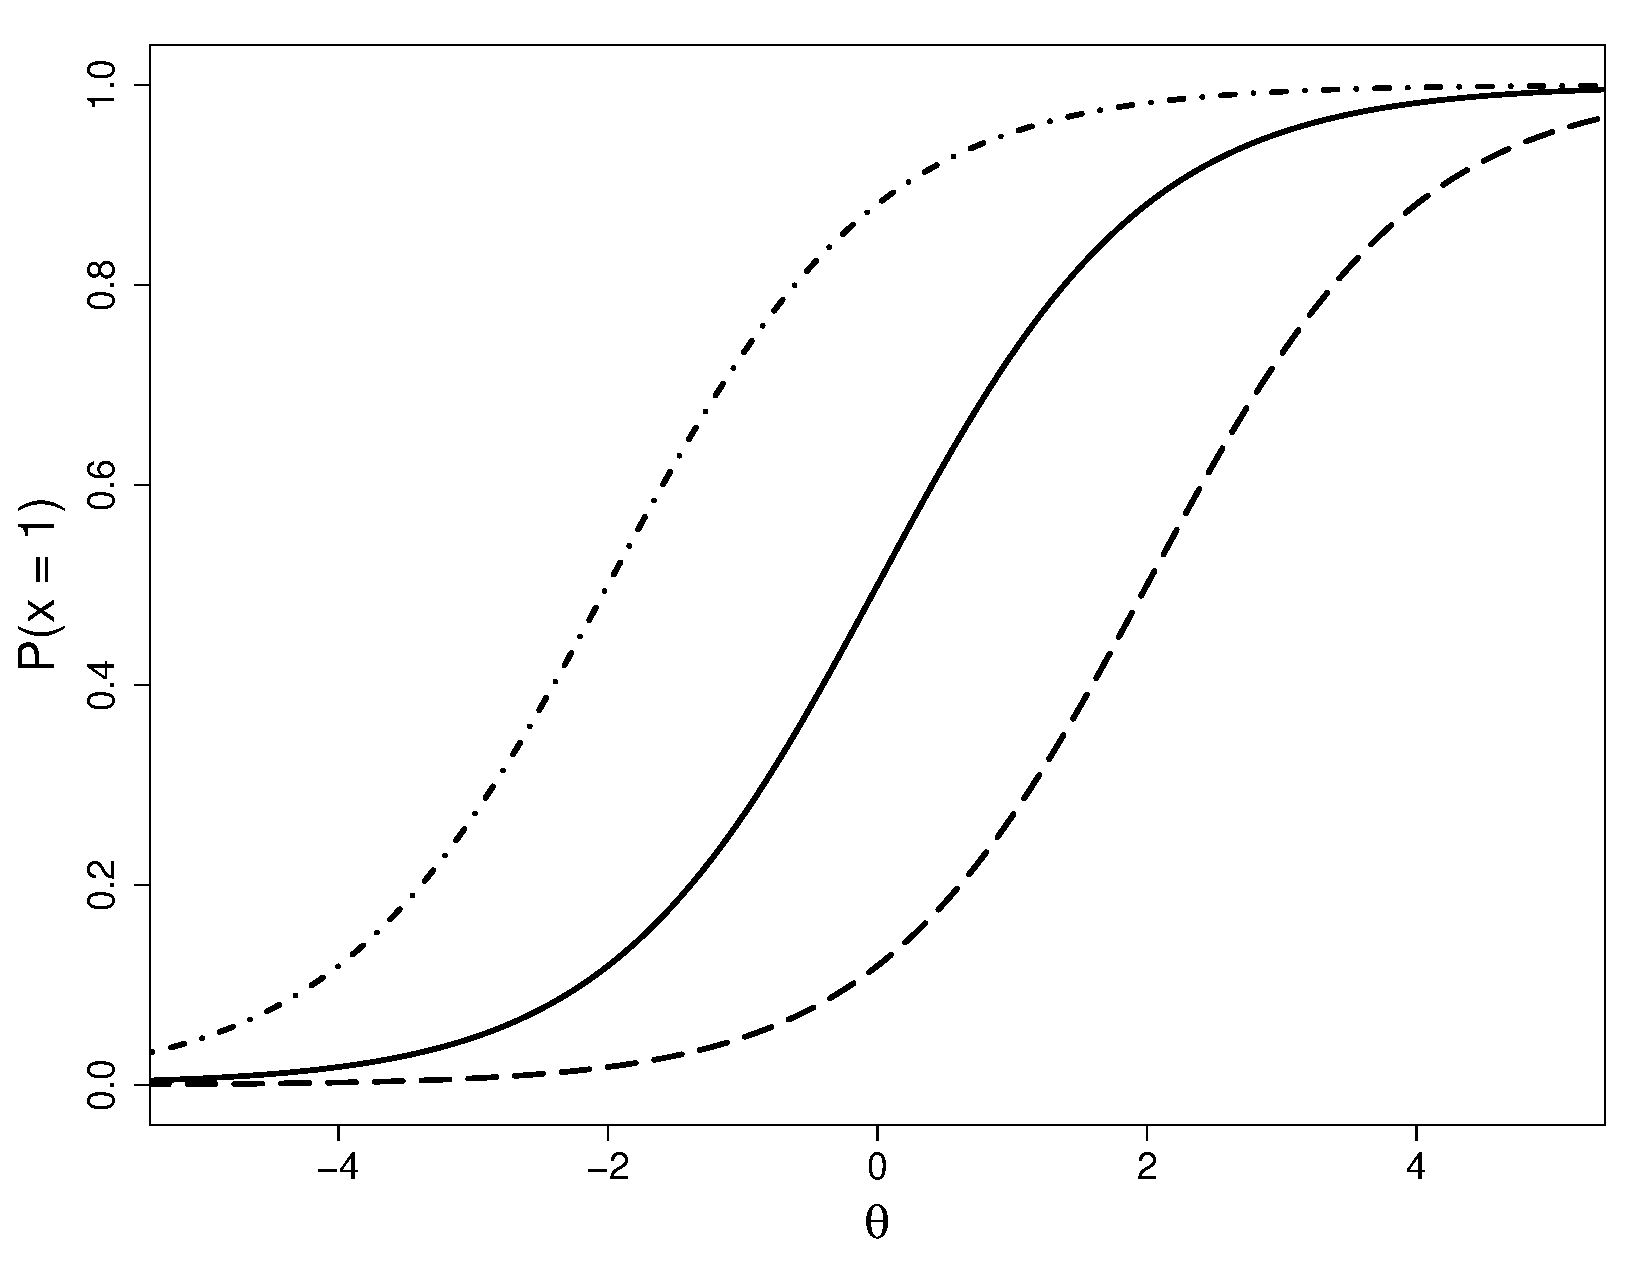
\includegraphics[width=\linewidth]{OnePL.pdf}
		\caption{1PL Model.}
		\label{subfig:1pl}
	\end{subfigure}
	\begin{subfigure}{0.45\linewidth}
		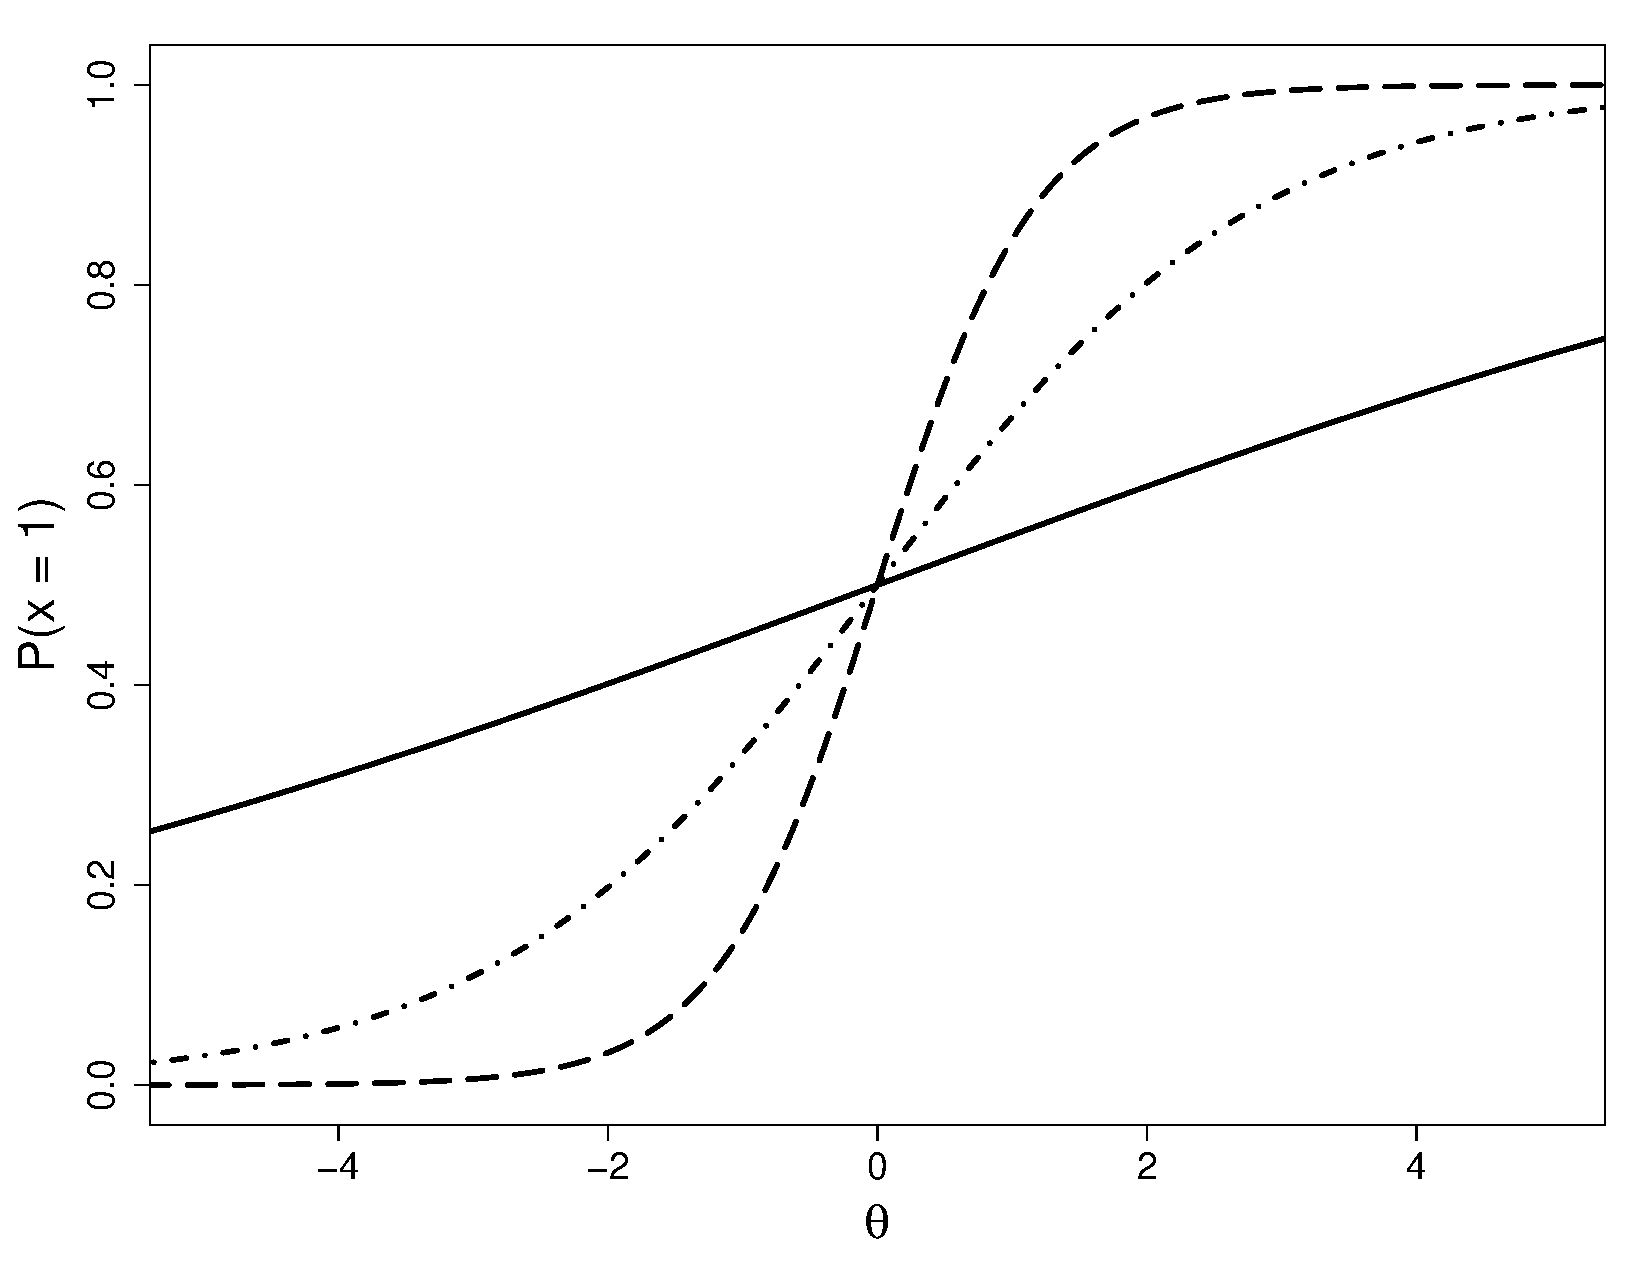
\includegraphics[width=\linewidth]{TwoPL.pdf}
		\caption{2PL Model.}
		\label{subfig:2pl}
	\end{subfigure}
	\begin{subfigure}{0.45\linewidth}
		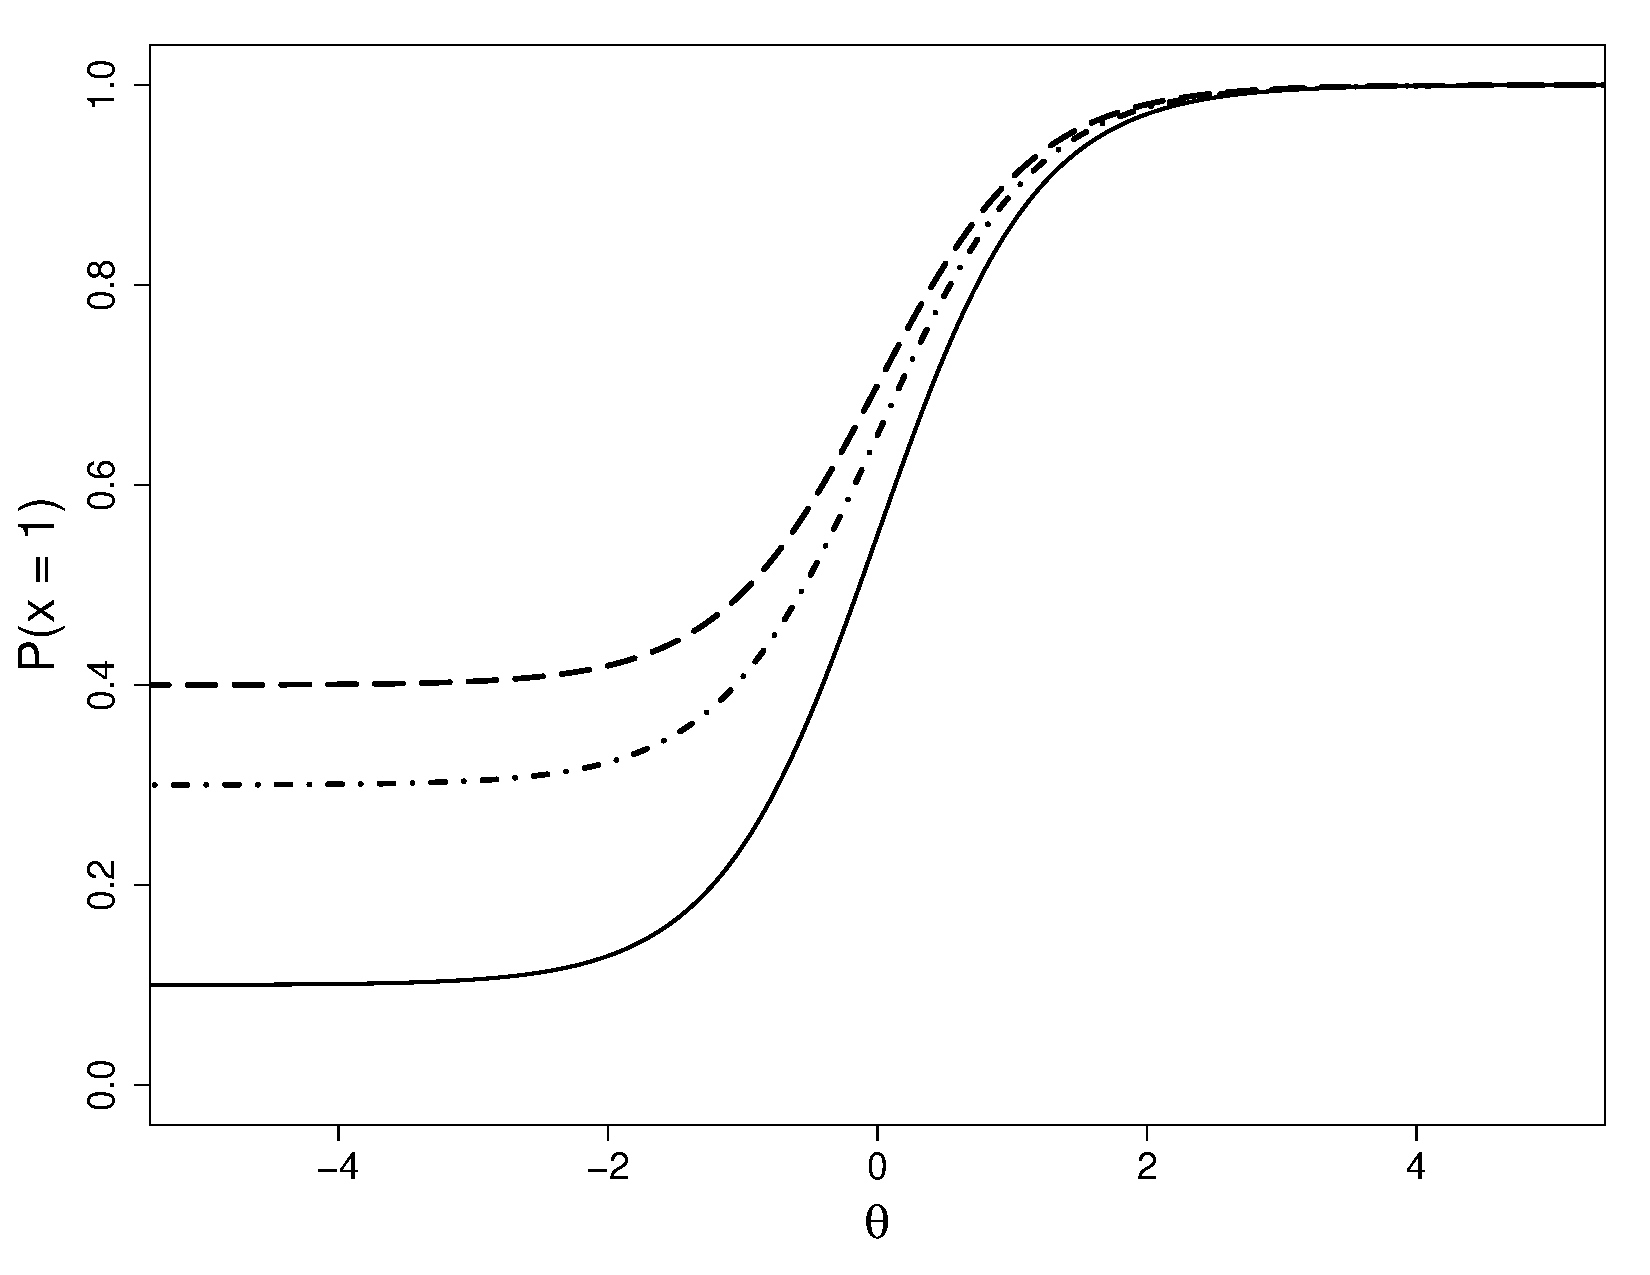
\includegraphics[width=\linewidth]{ThreePL.pdf}
		\caption{3PL Model.}
		\label{subfig:3pl}
	\end{subfigure}
	\begin{subfigure}{0.45\linewidth}
		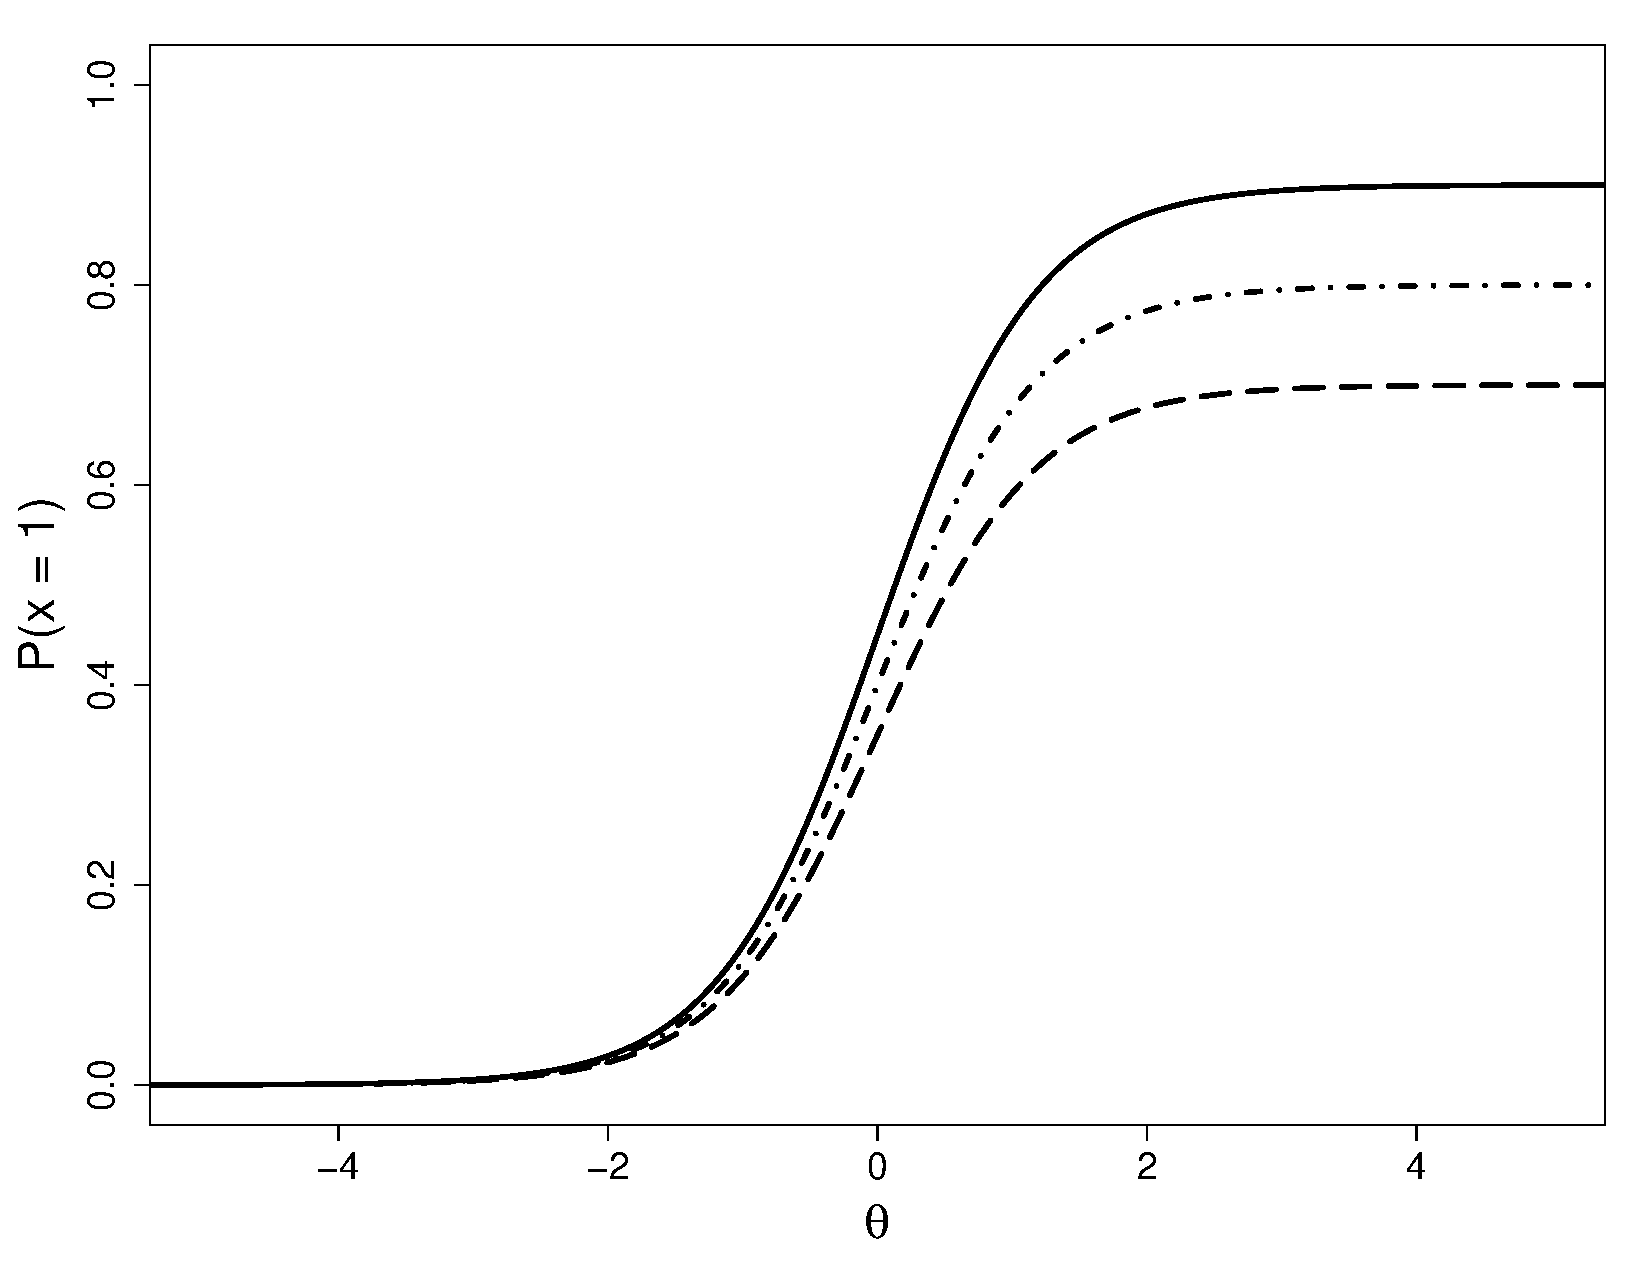
\includegraphics[width=\linewidth]{FourPL.pdf}
		\caption{4PL Model.}
		\label{subfig:4pl}
	\end{subfigure}
	\caption{\label{fig:IRTmodels} Item Characteristics Curves (ICCs) obtained with different IRT models.}
\end{figure}

As it can be seen in Figures \ref{subfig:1pl} and \ref{subfig:2pl}, the ICCs of the items approach 0 (for low levels of $\theta$) and 1 (for high levels of $\theta$), regardless of the parameters defining the characteristics of the items. This is because the 1PL and the 2PL models assume a lower asymptote at 0 (i.e., the value taken by the function as $\theta$ approaches $- \infty$) and an upper asymptote at 1 (i.e., the value taken by the function as $\theta$ approaches $+ \infty$). A lower asymptote at 0 is also assumed by the Rasch model.
The assumption of the lower asymptote approaching zero implies that respondents with extremely low levels of ability have an extremely low probability of endorsing the correct response. 
Conversely, assuming an upper asymptote of 1 implies that respondents with extremely high levels of ability have an extremely high probability of endorsing the correct response. 
However, there might be cases in which respondents with an extremely low level of ability choose the right response  out of luck (lucky guess), or that respondents with an extremely high level of ability choose the incorrect response  out of distraction (careless error). 
In the first case, the lower asymptote cannot approach zero anymore, since even respondents with a level of ability that approaches $- \infty$ have a probability of providing the correct response higher than 0. 
In the latter one, the upper asymptote has to be moved downward because even the respondents with a level of ability that approaches $+ \infty$ have a probability of correctly endorsing the correct response lower than 1. 

The 3PL and 4PL models have been introduced for modeling these occurrences, respectively.

The 3PL model (Equation \ref{eq:3pl}) \cite{lord}  adds a third parameter ($c$) to explain the response behavior: 
\begin{equation}\label{eq:3pl}
	P(x_{ps} = 1 | \theta_p, b_s, a_s, c_s) = c_s + (1-c_s)\frac{exp[a_s(\theta_p - b_s)]}{1 + exp[a_s(\theta_p - b_s)]},
\end{equation}
where $c_s$ is the probability that a respondent with a low level of ability guesses the correct response. 
The ICCs of three items with the same levels of difficulty and the same discriminating power are reported in Figure \ref{subfig:3pl}. As it can be immediately noted, the lower asymptote does not approach 0 anymore.
	The $c_s$ parameter moves upward the lower asymptote, and it represents the probability that a respondent with an extremely low ability will correctly answer an item with difficulty $b_s$.
The solid line item presents a low guessing parameter, according to which even respondents with an ability level below the item difficulty have about a 10\% chance of endorsing the correct response. 
	The most problematic item is the one represented by the dashed line. In this case, even respondents with a level of ability extremely lower than the item difficulty have a probability of endorsing the correct response as large as 40\%.

The 4PL model (Equation \ref{eq:4pl}) \cite{4plbarton} adds a fourth item parameter ($e$) to describe the response behavior:
\begin{equation}\label{eq:4pl}
	P(x_{ps} = 1 | \theta_p, b_s, a_s, c_s, e_s) = c_s + (e_s-c_s)\frac{exp[a_s(\theta_p - b_s)]}{1 + exp[a_s(\theta_p - b_s)]},
\end{equation} 
where $e_s$ represents the probability that a respondent with an extremely high level of ability will incorrectly answer an easy item (i.e., careless error). 
The ICCs of three items with the same difficulty, discriminating power, and guessing (set at 0 for illustration purpose) are depicted in Figure \ref{subfig:4pl}.
	In this case, it can be noted that the ICCs of the items does not approach 1 anymore: The upper asymptote is defined by the parameter $e$. 
	The ICC of the solid line item indicates that even for respondents with an extremely high level of ability, the probability of endorsing the correct response is about 90\%. 



\subsection{The Rasch model}

%The Rasch model \cite{rasch1960} is not a special case of the 2PL model, even though it is mathematically equivalent to the 1PL model \cite{demars}.
%The Rasch model is specified in terms of \emph{log-odds} (i.e., \emph{logits}, the natural logarithm of the odds).
The 1PL model and the Rasch model are mathematically equivalent. Only the notational system for their parameters is different. In the Rasch model, the item parameter is described by the Greek letter $\delta$ and the person's parameter is described by $\beta$. 
In this section, the typical notation of the Rasch model is used. However, in Section \ref{sec:random} the notation typical of IRT models is used to distinguish the Rasch model parameter estimates from the estimates of the log-normal model and those of the GLMMs.

The starting point for the development of the dichotomous Rasch model \cite{rasch1960} involves the engagement of a person $p$ on an item $s$ to produce a response $x_{ps}$ \cite{andrich}. 
The engagement between the person and the item results from a single variable that is a common property shared by both the person and the item. The item variable is supposed to trigger the same person variable in all respondents.
%Therefore, the same person property is triggered in all persons administered with that specific set of items.
For instance, for assessing mathematics proficiency the items must contain some degree of mathematics ability. To give the correct response, persons must engage with the mathematics proficiency required by the item.   
%The properties of the items should trigger the same variable in all persons. For example, in a math proficiency test, the person's property under investigation is the math ability, which is the variable that should be used for giving the correct response to each item. Each item should be able to trigger this ability in each person.

The engagement between the person and the item results in the observed responses $x_{ps}$, which can be represented in a $P$ ($p \in \{1, \ldots, P\}$, persons) $\times$ items $S$ ($s\in \{1, \ldots, S\}$, items) response matrix $\bm{X}$ (Table \ref{tab:rasch}). 

\begin{table}[h!]
	\centering
	\caption{\label{tab:rasch} Response matrix $P \times S$, starting point for the estimation of the Rasch model.}
	\begin{tabular}{p{1cm}  p{1cm}  |p{1.5cm}  p{1.5cm} p{1.5cm} p{1.5cm} p{1.5cm} p{1.5cm} | p{1.5cm}}
		& \multicolumn{1}{l}{} & \multicolumn{6}{c}{Items} & \multicolumn{1}{c}{} \\
		& \multicolumn{1}{c}{} & \multicolumn{1}{l}{1} & \multicolumn{1}{l}{2} & \multicolumn{1}{l}{$\ldots$} & 
		\multicolumn{1}{l}{$k$} & \multicolumn{1}{l}{$\ldots$} & \multicolumn{1}{l}{$s$}& \\
		\cline{3-8}
		\multirow{8}{*}{Persons} & 1 & $x_{11}$ & $x_{12}$ & $\ldots$& $x_{1k}$ & $\ldots$ & $x_{1k}$ & $r_1$ \\
		&	2 & $x_{21}$ & $x_{22}$ & $\ldots$& $x_{2k}$ & $\ldots$ & $x_{2k}$ & $r_2$ \\
		&	$\vdots$ & $\ldots$ & $\ldots$ & $\ldots$ & $\ldots$ & $\ldots$ & $\ldots$ & $\vdots$ \\
		&	$v$ & $x_{v1}$ & $x_{v2}$ & $\ldots$& $x_{vk}$ & $\ldots$ & $x_{vk}$ & $r_v$ \\
		&	$\vdots$ & $\ldots$ & $\ldots$ & $\ldots$ & $\ldots$ & $\ldots$ & $\ldots$ & $\vdots$ \\
		&	$p$ & $x_{p1}$ & $x_{p2}$ & $\ldots$& $x_{pk}$ & $\ldots$ & $x_{ps}$ & $r_p$ \\
		\cline{3-8}
		& \multicolumn{1}{c}{} & $s_1$ &  $s_2$ & $\ldots$ & $s_k$ & $\ldots$  & \multicolumn{2}{l}{$s_s$}\\ 
	\end{tabular}
\end{table}

Each cell represents the response of person $p$ to item $s$. 
The response is a dichotomous response that can take only the values $x_{ps} = 0$ (incorrect response) or $x_{ps} = 1$ (correct response). 

The across-columns sum $r_p$ (i.e., number-correct) represents the total score of each respondent (i.e., the total number of correct responses given by the respondent), regardless of the specific pattern with which the correct responses were given.
The number-correct is a sufficient statistic for estimating the person's parameter $\beta$ \cite{wright1979, wright1997}. 
Two respondents might have the same number-correct obtained with different patterns of correct responses. Since the specific pattern is not important for the determination of the number-correct, the two respondents with the same number-correct obtained with different patterns will have the same person estimate $\beta$. 
This feature distinguishes the Rasch model from other IRT models. For instance, in the 2PL model two respondents with the same number-correct might not have the same level of $\theta$ because the relationship between the item and the respondent's parameters is moderated by the discriminating power of the item $a_s$, hence the specific response pattern is important for the estimation of the person parameter.

The across-rows sum $s_s$ (i.e., proportion-correct) represents the total score of each item (i.e., number of correct responses obtained by each item), regardless of the specific pattern with which the responses were obtained.  The proportion-correct is a sufficient statistic for estimating the item difficulty parameter $\delta$.
Two items might have the same proportion-correct resulting from different pattern of responses, but since the specific pattern is not relevant for the determination of the proportion-correct, the two items will have the same item estimate $\delta$.

The observed response in each cell $x_{ps}$ hence depends on both persons’ characteristics and items characteristics. 
The characteristics of both persons and stimuli can be located on a specific point of the latent trait, which is the common variable they share. 
The location
of each respondent $p$ on the latent trait is described by the parameter $\beta_p$. The location of each stimulus on the latent trait is described by parameter the $\delta_s$. 
While the observed response for each combination of $p \times s$ can take only the value 0 and 1, the parameters $\beta_p$ and $\delta_s$ can take any real value from $- \infty$ to $+ \infty$. 

The great advantage of the Rasch model and of IRT models in general is represented by the person and item characteristics located on the same latent trait, which allows for directly compare the person and item estimates.
%The fact that persons and items are located on the same latent trait is the great advantage of the Rasch model, and IRT models in general. 
%By sharing the same latent trait, it is possible to directly compare the persons' estimates with the items estimates. 
A measure of the distance between the person's location and the item location can hence be obtained. Therefore, it is possible to predict the probability that a person with a certain level of $\beta$ has of correctly respond to an item with a certain level of $\delta$. 
Since the observed response is a function of the respondent and stimulus characteristics located on the same latent trait, it can be posited that a respondent would correctly respond to the stimuli located below his/her level of ability $\beta_p$ (i.e., the probability of a correct response is higher than 50\%): 
\begin{equation}\label{eq:rasch1}
	\text{If} \, (\beta_p - \delta_s) > 0 \, \text{then} \, P(x_{ps} = 1) > 0.50.
\end{equation}

Also the opposite holds true. When the location of the item is above the location of the person, the probability that a correct response is given is below 50\%: 
\begin{equation}\label{eq:rasch2}
	\text{If} \, (\beta_p - \delta_s) < 0 \, \text{then} \, P(x_{ps} = 1) < 0.50.
\end{equation}

As Equations \ref{eq:rasch1} and \ref{eq:rasch2} clearly illustrate, the probability of a correct response depends on the difference between the respondent and item parameters. 
However, the probability of a correct response is bounded between 0 and 1, while the parameters, and hence their difference, can vary between $- \infty$ and $+ \infty$. 
The difference between the respondent and item parameters can be forced to only positive numbers by using the exponential function: 
\begin{equation}\label{eq:raschprob}
	0 \leq exp(\beta_p - \delta_s) < + \infty
\end{equation}
Still, in Equation \ref{eq:raschprob} the difference between the person ability and the item difficulty is allowed to take any positive value from 0 to $+ \infty$. As such, it cannot be used to predict a probability varying between 0 and 1. 
To allow for the prediction of the probability of a correct response given respondent ability and item difficulty, the difference between their parameters need to be mapped on the same scale of the probability. Thus, Equation \ref{eq:raschprob} can be standardized by $1 + exp(\beta_p - \delta_s)$, so that the probability for a correct response for a given $\beta_p$ and a given $\delta_s$ can be expressed as: 
\begin{equation}\label{eq:raschcorrect}
	P(x_{ps} = 1 | \beta_p, \delta_s) = \frac{exp(\beta_p - \delta_s)}{1 + exp(\beta_p - \delta_s)},
\end{equation}
which is the typical formulation of the Rasch model for the probability of a correct response. 

The Rasch model was originally formulated in terms of odds and \emph{log-odds}. The odds are the ratio between the probability of success (correct response) and the probability of failure (incorrect response). The \emph{log-odds} are the logarithm of the odds. 
The Rasch model assumes a logistic probability function, and the measurement units of the respondent parameters, the item parameters, and their difference, are the \emph{logits}.
Equation \ref{eq:raschcorrect} can be rewritten in terms of \emph{log-odds} as:
\begin{equation}\label{eq:raschcorrectlog}
	\beta_p - \delta_s = \text{ln}\left(\frac{P(x =1|\beta_p, \delta_s)}{1 - P(x =1|\beta_p, \delta_s)}\right).
\end{equation} 
By applying the properties of the logarithms to Equation \ref{eq:raschcorrect}, the Rasch model can be rewritten as: 
\begin{equation}\label{eq:inverseraschInverse}
	P(x_{ps} = 1 |\beta_p, \delta_s) = \frac{1}{exp(\delta_s - \theta_p)}.
\end{equation}
Regardless of the specific equation used for expressing the Rasch model, the only thing that matters for the estimation of the expected probabilities is the difference between $\beta_p$ and $\delta_s$. 
This difference expresses the distance between the location of the respondent $p$ from the location of the stimulus $s$ on the latent trait. 
Therefore, the   probability  of a correct (incorrect) response changes according to the distance between the respondent and item locations. The probability of a correct response is 50\% when the respondent location is equal to the item location. 
The variance for the expected probabilities of the responses when the locations of the respondent and the stimulus correspond is maximized, because the probability of giving the correct response is equal to the probability of giving the incorrect response ($P(x_{ps}=1) = P(x_{ps}=0)= 0.50$).

The more the location of a respondent on the latent trait is above the location of the item, the higher the probability of observing a correct response (see Equation \ref{eq:rasch1}). 
Similarly, the less the distance between the location of the respondent and that of the item on the latent trait, the lower the probability of observing a correct response.
Also the opposite holds true. 
The more the location of the respondent is below the item location, the higher  the probability of an incorrect response (see Equation \ref{eq:rasch2}), and, conversely, the less the location of the respondent is below the location of the item, the lower the probability of an incorrect response.
The relationship between the respondent parameter and the item parameter defines the cumulative nature of the Rasch model. 


%The measurement units of the difference between respondents and stimuli parameters are the \emph{logits}, and the RThe logistic probability function is the probability function on which the Rasch model rests. 

%The implications and assumptions of the Rasch model are briefly outlined in the following Paragraphs.
%The Rasch model implies both a single dimension, where respondents' and items characteristics can be placed, and, related to that, the statistical independence of responses (i.e., the probability of giving the correct response to different items is equal to the product of the probability of correctly answering each of them). 

The Rasch model is based on three main assumptions, namely linearity of the scores, comparison invariance, and local independence. These assumptions are briefly outlined in the following paragraphs, with a specific focus on conditional independence and on the consequences of its violation. 

\paragraph{Linearity of the scores.}
The linearity of the scores is obtained with the logarithm transformation of the odds. By applying this transformation, the person parameters and the item parameters are placed on the same continuous latent trait. The logarithm transformation of the odds defines the measurement units of the latent trait (i.e., the \emph{logits}), which allow for interpreting the scores on an interval scale.

The linear transformation of the relationship between the respondent and stimulus parameters allows for setting the lowest parameter observed equal to 0, without losing the original relationship between the estimates. Consequently, comparison invariance (described in the following paragraph) assumption is satisfied.

\paragraph{Comparison invariance.}
The comparison between any two persons is independent from the set of items on which the comparison is based, as well as independent from the comparison between any other two persons. 
The same holds for the items. The comparison between any two items is independent from the respondents on which the comparison in made, as well as from the comparison between any other two persons.

The comparisons are invariant in the sense that the comparison between the persons only depends on the ability parameters of those two persons, and the comparison between the items only depends on the items parameters. 


\paragraph{Local independence.}\label{par:local}

According to the Rasch model, a person with a  level of ability $\beta$ greater than the item difficulty $\delta$ has a greater probability of responding  correctly than incorrectly to that item. 
Conversely, a person with a level of ability $\beta$ lower than the item difficulty $\delta$ has a higher probability of responding incorrectly than correctly to that item. 
As such, the variability between the item responses can  be explained in terms of the person ability $\beta$, which can be considered as the source of general dependence between the items. Once the effect of the person ability is accounted for, any other relationship between the items should disappear. 
The potential of the person parameters $\beta$ to explain all the variability between the responses is called local independence \cite{andrich}, according to which once the effect of the person parameter is accounted for, any other relationship between the item disappears.   

The statistical independence of the responses implies that the probability of correctly responding to different items is equal to the product of the probabilities of answering each of them correctly. The local independence of the responses can be formalized as: 
\begin{equation}\label{eq:local}
	P(\bm{X}) = \prod_p \prod_s \, P(x_{ps}),
\end{equation}
where $\bm{X}$ is the $P \times S$ matrix of the responses. 

The violation of the assumption of local independence can happen in two main instances, either by involving multidimensionality of the latent trait of the respondents or response dependence. 
The consequences of the local independence violation due to either multidimensionality or response dependence move in opposite directions but they both result in less reliable estimates of the parameters and, consequently, in a less accurate prediction of the probability of observing a correct response given respondent ability and item difficulty.

Unidimensionality posits that the item responses can be explained by considering only one latent trait dimension, shared by both the respondents and the items. Unidimensionality is the basic underlying assumption of the Rasch model.
Conversely, multidimensionality refers to those cases in which there are unexpected person's parameters other than $\beta$ involved in the responses to the items. 

Multidimensionality is indeed a property of many different scales used for psychological assessment. For instance, the Big Five Questionnaire \cite{bigfive} is a questionnaire for the assessment of the Big Five personality traits, composed of different sub-scales. 
The items in each of the 5 sub-scales are aimed at assessing one of the 5 personality traits posited by the Big Five theory (i.e., agreeableness, extroversion, openness to experience, neuroticism, conscientiousness). The items can be grouped together according to the personality trait they aim for. 
As such, they show a between--sub-scale variability which cannot be explained by only one person’s parameter $\beta$. 
Multidimensionality can also raise from stimuli linked by common attributes such as a common item stem, common stimulus materials, or common item structures \cite{andrich}. 
Consequently, stimuli will display a variability due to other characteristics that cannot be explained just in terms of ability parameters $\beta$. 

Response dependence \cite<i.e., for a fixed person, hence for a fixed level of ability $\beta$, the response to an item might depend on the response to a previous item;>{andrich} violates the assumption of local independence as expressed in Equation \ref{eq:local}. 
Since the responses to the items share other sources of variability beyond respondent ability, they cannot be considered as independent events anymore.  Consequently, the probability that each item has of getting a correct response cannot be multiplied with the probability of getting a correct response of another item. 

Response dependence might emerge in at least two instances. One case might be when the response given to an item is used as a clue for responding to subsequent items. 
Response dependence might also arise during the performance at computerized task, when the response to an item leaves a carry-over effect on the response to the subsequent item \cite{Westfall2014}. 
In this instance, the variability at the item level is affected by new sources of variability, mostly composed of error variance. 

The violation of the assumption of local independence affects the fit of the data to the model \cite{andrich}, and produces unreliable estimate of the parameters \cite<e.g.,>{Barr2013, judd2012}. 
When local dependence is due to multidimensionality of the person latent trait, extra sources of random noise are added to the data. The error variance is hence increased, producing less accurate and reliable predictions. 
When local dependence is due to response dependence, the similarity of the responses of persons across items is higher than in conditions of no response dependence. This leads to a decrease in the error variability. As such, the probabilistic nature of the Rasch model is lost in favor of a more deterministic one, and responses can be explained with a Guttman-like process.  


\section{Modeling time responses}\label{sec:lognormal}

By modeling response times within an IRT approach, an interaction between the parameters defining the person accuracy and the time responses is implicitly assumed. 
This is nothing else than the speed-accuracy trade-off also reported in previous analysis of the IAT data \cite<e.g.,>{Klauer2007}. 


Traditionally, in IRT modeling the speed-accuracy trade-off has been expressed by adopting a regression parameter for the ability of the respondents on their response times. 
Consistently with IRT models on accuracy responses, the contribution of the items is fundamental in determining the observed time responses and it is commonly assumed that more difficult items require for more time to get a response. As such, item parameters are needed to describe the time absorbing power of the item \cite{van2006}.


\subsection{The log-normal model}

A log-normal model for the analysis of the response times to a test has been introduced by \citeA{van2006}. The log-normal model is part of a hierarchical model for the modeling of accuracy and time responses in an IRT framework \cite{VanDerLinden2009}. 
According to \citeA{van2006, VanDerLinden2009}, the models for the accuracy responses (i.e., any of the IRT models presented in the previous section) and those for the time responses can be employed individually for distinct analysis of the accuracy and time responses to a test. 
The advantage of using the hierarchical approach in \citeA{VanDerLinden2009} is that the relationship between the parameters of the IRT model and the time parameters can be studied and understood at a second (combined) level of modeling. 

 As its name suggests, the log-normal model assumes a normal density distribution for the logarithm of the time responses. 
The decision to use the log-normal family can be traced to its good fit to the observed data in previous studies \cite<e.g.,>{thissen, van2006}. More trivially, it comes natural to model with a normal distribution (defined over the entire real continuum) the log transformation of a variable that is a non-negative variable by definition (the response times) \cite{van2006}.

The structure of the original formulation of the log-normal model is analogous to the one of the 2PL IRT model in Equation \ref{eq:2pl} for mainly three reasons. 
First, both the 2PL and the log-normal models impose the same structure on the mean of the distribution of the binary response variable and on the mean of the distribution of the continuous variable, respectively. 
In both cases, the mean is represented by the difference between the parameters of the respondent and those of the item, moving in opposite directions.
Second, both models assume a parameter that changes the relationship between the item and respondent parameters, namely a discrimination parameter. Further details on the effect and on the interpretation of the discrimination parameter on the time responses are illustrated after the mathematical specification of the log-normal model. 
Finally, given the nature of the distribution of the response times (it is bounded at 0), the log-normal model does not need the definition of a lower asymptote (i.e., the guessing parameter of the 3PL model in Equation \ref{eq:3pl}).

Let $t$ be the realization of a random variable $T$ and $t_{ps}$ the response time of a respondent $p$ to an item $s$. 
The log-normal model assumes a normal density distribution of the log-response times as follows: 
%
\begin{equation}\label{eq:log}
	f(t_{ps}| \tau_p, \delta_s) = \frac{\alpha_s}{t_{ps}\sqrt{2\pi}}exp\left\{ -\frac{1}{2}[\alpha_s(ln\;t_{ps} - (\delta_s - \tau_p))]^2 \right\}.
\end{equation} 
%
As in IRT models, both the respondent and stimulus parameters $\tau_p$ and $\delta_s$ are allowed to vary between $- \infty$ and $+ \infty$, and are located on the same latent trait. 
Although the sign of the person parameter $\tau_p$ is reversed, the mean of the distribution of Equation \ref{eq:log} resembles the one of the 2PL in Equation \ref{eq:2pl}. 
The change in the sign of the respondent parameter $\tau_p$ allows for interpreting the parameter as a speed parameter, according to which, the larger the value of $\tau_p$, the faster the responses given across items (i.e., the respondent tends to spend less time on the items). 
Parameter $\delta_s$ describes the time intensity (or time consumingness)  of an item, which is the time the stimulus requires to be responded. The larger the value of $\delta_s$, the higher the amount of time respondents need to give the response.
Parameter $\alpha$ (i.e., the reciprocal of the standard deviation of the normal distribution) is the discrimination parameter of the model. An high value of $\alpha_s$ means less dispersion of the log-response time distribution on item $s$. Consequently, it can be said that the item has a better discrimintating ability between different respondents with different levels of speed. 
Parameter $\alpha_s$ affects the relationship between the respondent speed $\tau_p$ and the item time intensity $\delta_s$ parameters, similarly to what happens when parameter $a_s$ changes in the 2PL model. 
If the value of $\alpha_s$ increases, the distributions of the log-time responses for any two values of the speed parameter show less overlap. 

The 1PL model in Equation \ref{eq:1pl} can be considered as a constrained model deriving from the 2PL model in Equation \ref{eq:2pl}. 
The constraint is imposed on the discrimination parameter $a$, which is forced to be equal across all items (1PL, Rasch model). 
A similar reasoning can be done for the log-normal model, by forcing $\alpha_s$ to be equal for all items $s$ ($\alpha_s = \alpha$ for all $s$, $s \in \{1, \ldots S\}$).
This constraint results in a parametrization of the log-time responses similar to  the 1PL/Rasch model parametrization of the accuracy responses.
%The former constraint brings a parametrization similar to the one of the 1PL model, the latter one can be equated to the parametrization provided by the Rasch model. 
In the empirical application in \citeA{van2006}, both a non-constrained and a constrained version of the log-normal model were tested in terms of goodness of fit to the data. 
The normal analogs of the non-constrained and constrained models were tested as well. 
The normal models were the ones showing the worst goodness-of-fit, while constraining $\alpha$ to be equal across all items did not affect the  goodness-of-fit of the log-normal models. 


\section{Linear Mixed-Effects Models}

As illustrated in the previous sections, an IRT (or Rasch) approach for modeling both accuracy and  time responses provides a detailed information on the parameters that determine the accuracy and time responses. 


The use of a log-normal model can overcome the issues related to the discretization of the response times for the application of the Many Facet Rasch Model in Section \ref{sec:mfrm}. 
The use of a separate model for accuracy responses within an IRT or Rasch framework allows for obtaining useful and detailed information from accuracy data as well. Importantly, the accuracy and log-time models present a similar parametrization of the data.  
Potentially, the estimates obtained from the two models can be combined at a second level of modeling by using a hierarchical approach as that illustrated in \citeA{VanDerLinden2009}. 

Despite this approach sounds promising, it cannot account for the fully-crossed design of the IAT data and its related sources of dependency. As thoroughly illustrated in the introduction (see Section \ref{sec:cross}), the fully-crossed design of the IAT comes with several sources of variability at different levels. These sources of variability generate dependencies at the level of the single observations that violate the assumption of conditional independence. 
Conditional independence is not only a necessary assumption for the application of the Rasch model, but a basic assumption needed for obtaining reliable results with any statistical analysis.
Violating the assumption of conditional independence brings to biased parameter estimates which can in turn lead to an inflated probability of committing Type I error or to an underestimation of the importance of the experimental conditions \cite{Barr2013, judd2012,mc1989}. 

Linear Mixed Effects models (LMMs) are the most straightforward way to deal with this data structure.
Moreover, LMMs allow for concurrently considering both the respondents and the stimuli as random factors with the specification of the appropriate random structure. 
As such, the issues concerning the decision to follow either  a \emph{by-participant} approach or a \emph{by-stimulus} approach for performing the analyses is overcome.

The specification of the random structure makes possible to decompose the error variance into different levels, which corresponds to the levels where the uncontrolled sources of random variation can be reasonably found \cite{Doran2007}. These levels can be understood as the random effects of the model, which reflect the assumptions on the structure of dependency created by the random variability at  different levels. As such, the multilevel structure of the data is accounted for \cite{Barr2013}.

LMMs can be applied to both continuous data, such as the log-transformation of the response times, and to dichotomous responses. In the latter case, a Generalized Linear Mixed-Effects Model (GLMMs) is needed, with the appropriate link function expressing the relationship between the linear combination of the predictors (i.e., the linear component of the model) and the observed response. 


\subsection{Generalized Linear Mixed-Effects Model and Rasch Model}

In a Generalized Linear Model (GLM), the linear predictors are not directly related to the observed response, and they need to be linked together with a specific function (i.e., \emph{link function}). 
The type of link function depends on the nature of the observed variable \cite{{mc1989}}.

For the illustration of the structure of the GLM, and of its expansion to include random effects, we focus on the case of binomial responses $x_{ps} \in \{0, 1\}$, describing the accuracy responses at the IAT. 

The linear combination of the predictors is defined by the model matrix $\bm{X}$, expressing the form of the model, and it determines the linear component of the model. 
The linear component is defined for each cell of the $P \times S$ $\bm{X}$ matrix, and it is denoted with $\eta_{ps}$. 

The natural link function $g$ that relates the observed binomial responses with the linear component of the model $\eta_{ps}$ is the \emph{logit} \cite<the logarithm of the odds,>{mc1989}, and it yields a probability value $\mu_{ps}$:
%When the observed responses are binomial responses, the natural link function $g$ \cite{mc1989} that relates the linear component $\eta_{ps}$ with the expected values of $x_{ps}$ is the \emph{logit}. 
\begin{equation}\label{eq:logit}
	\eta_{ps} = logit(\mu_{ps}) = ln\left( \frac{\mu_{ps}}{1 - \mu_{ps}}\right),
\end{equation}
where $\mu_{ps}$ is the probability of a correct response associated to each observed response $x_{ps}$.

Each link function is an invertible function. The inverse of the \emph{logit} link function is expressed as:
\begin{equation}\label{eq:inverse}
	\mu_{ps} = logit^{-1}(\eta_{ps}) = \frac{1}{1 + exp(-\eta_{ps})}.
\end{equation}
The structure of the inverse \emph{logit} link in Equation \ref{eq:inverse} can be equated to the Rasch formulation in Equation \ref{eq:inverseraschInverse}. 
As such, a Rasch parametrization of the data by using a GLM on binomial responses with a \emph{logit} link function can be obtained \cite{DeBoeck2011, Doran2007, Gelman2007}. 

From now on, to distinguish the parameters of the Rasch model from the parameters obtained with the LMMs the former ones will be denoted with $\theta_p$ and $b_s$, indicating the respondent  and stimulus parameters, respectively.
%the parameters of the Rasch model will be referred to as $\theta_p$ and $b_s$, referring to respondents' ability and stimuli difficulty, respectively, to distinguish them from the parameters obtained with the LMMs.

%The interpretation of the stimulus parameter $\delta_s$ is nonetheless reversed. 
%In the inverse \emph{logit} function of Equation \ref{eq:inverse}, the relationship between respondent's charactertis and item difficulty has changed becoming and additive, rather than a differential, relationship. 
%As such, the item parameter $\delta$ can no longer be interpreted as an impediment property (difficulty) of the stimulus but it should be interpreted as a facilitation property of the stimulus (easiness) \cite{DeBoeck2011, Doran2007}.

When there are reasons to believe that there  are sources of variability generating dependencies between the observations, such as in the IAT case, random effects addressing the uncontrolled  random variability should be included in the model matrix of the linear component. 
By doing so, the error variance is partitioned in different levels as defined by the random effects. 
The partitioning of the error variance into specific effects makes the sources of error variance controllable and accountable for \cite{Doran2007}.

The $\bm{X}$ matrix that defines the linear component of the GLM needs to be extended to include the random factors. 
The linear component hence takes on the form:
\begin{equation}
	\eta = \bm{X}\beta + \bm{Z}d,
\end{equation}
where $\beta$ indicates the coefficients for the fixed effects (intercepts and slopes), $\bm{X}$ is the model matrix of the fixed effects $\beta$, $\bm{Z}$ is the $P \times Q$ matrix of the random effects (i.e., $Q$ is the dimension of the random effects vector), and $d$ is the vector of the random effects. 

The dimension $Q$ of $d$ is defined by the number of levels of each random factor, and their combinations. For instance, if respondents are considered as  random factors, the dimension $Q$ of the random effects vector will have as many levels as the number of respondents. 
Consequently, the dimension of $d$ can be potentially very large \cite{Doran2007}.
The distribution of the random effects is estimated as a multivariate normal distribution (i.e., $\mathcal{MVN}$) with mean 0 and a $Q \times Q$ variance-covariance matrix $\bm{\Sigma}$, which is determined by a single vector of parameters $\Gamma$ \cite{Doran2007}. 
The dimension of $\Gamma$ is usually rather small, and its size is determined by the number of random factors specified in the model, regardless of the number of levels they include.  
For instance, consider a model in which the respondents variability, the items variability, and the items variability in three different conditions are accounted for. In this model, five random factors are considered and their related random effects are specified. Specifically, a random effect for the respondents variability, one for the items variability, and one allowing for the multidimensionality of the stimuli variability in the three conditions are specified. 
The dimension of the vector parameter $\Gamma$ for this model is 5, and it remains 5, regardless of the number of respondents or items used.

The objective of LMMs is to estimate the parameters of the fixed effects as defined in vector $\beta$ and the parameters of the random effects as defined in vector $\Gamma$. Consequently, the parameters estimated for the random factors are not the parameters associated to each level of each factor, but the variances of the populations from which the random factors are drawn. Since $d$ does not directly refer to population parameters is denoted with a Latin letter instead of a Greek one. 
Nonetheless, a measure for each level of each random factor is obtained in the form of \emph{conditional modes}, which are the values maximizing the conditional density of the random effects given the vectors of fixed and random parameters and the observed data \cite{Doran2007}. 
The conditional modes describing the deviation of each random factor from the fixed factors are meta-parameters \cite{pastore}, and are usually referred to as \emph{Best Linear Unbiased Predictors} \cite<BLUP,>{pinheiro2006}. 

In the typical formulation of the Rasch model,  the respondent and stimulus parameters move in opposite directions. 
However, when the respondent and stimulus parameters of the Rasch model are obtained by using the GLMMs, their estimates move in the same direction, hence resulting in an additive effect.
The item parameter $b_s$ can no longer be interpreted as an impediment property  of the stimulus (difficulty) but it should be interpreted as a facilitation property of the stimulus (easiness) \cite{DeBoeck2011, Doran2007}. 
When both $\theta_p$ and $b_s$ are high, the probability of a correct response is high. 
When high values of $\theta_p$ are combined with low values of $b_s$, the probability of a correct response for each respondent is as much penalized as their ability cannot balance out the easiness of the stimulus. 

BLUP are used for the estimation of the Rasch model parameters from the GLMMs. 
The easiness estimates $b_s$ of the stimuli are obtained by adding the BLUP of each stimulus to the estimates of the fixed effects. 
In the IAT case, the higher the value of the stimuli easiness $b_s$, the easier the stimulus, meaning that it is easily recognized and sorted to the category to which it belongs.  
Similarly, adding the conditional mode of each respondent to the estimates of the fixed effects results in the estimation of  respondent ability parameters $\theta_p$. 
In the IAT case, the higher the value of $\theta_p$, the higher the ability of the respondent of correctly categorizing the stimuli. 


\paragraph{Log-normal model estimates.}

%The Rasch model estimates can be obtained by combining together the fixed component and the random component of the GLMMs applied to accuracy responses. 
%Instead of being governed by the difference between the respondents' ability and the stimuli easiness, the probability of a correct response is governed by the additive effect of the respondents' ability and the stimuli easiness. Consequently, the interpretation of the stimuli parameters $b_s$ changes.
%
%In a similar vein, 
The estimates of the log-normal model parameters can be obtained by combining the fixed factors to the random factors of the LMMs applied to the log-time responses.  
In the typical formulation of the log-normal model (Equation \ref{eq:log}), the mean of the distribution of the expected log-time responses is expressed by the difference between the time intensity parameters of the stimuli $\delta_s$ and the speed parameters of the respondents $\tau_p$ (i.e., $\delta_s - \tau_{p}$). 
In the LMMs, the mean of the distribution is defined by the additive effect between the respondent and stimulus characteristics, which move in the same direction. Consistently, the lower the value of the speed parameter $\tau_p$, the  higher the speed, and the lower the value of $\delta_p$, the lower the time the stimulus requires for getting a response. 

When respondents with a low value of $\tau_p$ (i.e., high speed) respond to items with a low value of $\delta_s$ (i.e., low time intensity), the response times are fast. 
When a respondent with a low value of $\tau_p$ encounters a stimulus with a high value of $\delta_s$, the speed of the response depends on the distance between the respondent's speed and the item time intensity.

\section{Random structures}\label{sec:random}
The random structures of the GLMMs and those of the LMMs are the same. The features differentiating the models are the assumptions on the error term $\varepsilon$ and the dependent variables. 
In the GLMMs, the error term is supposed to follow a logistic distribution (i.e., $\varepsilon \sim \mathcal{L}(0, \sigma^2)$, where $\mathcal{L}$ is used to denote the logistic distribution of the disturbance as in \citeA{Doran2007}) and the dependent variable is the accuracy response to each trial of the IAT. 
In the LMMs, the error term is supposed to follow a normal distribution (i.e., $\varepsilon \sim \mathcal{N}(0, \sigma^2)$), and the dependent variable $y$ is the log transformation of the time response to each trial of the IAT, regardless of whether the answer is correct or not.
The expected response $y$ for each observation $i$ ($i \in \{1, \ldots, n\}$)  for participant $p$ ($p \in \{1,\ldots, P\}$) on stimulus $s$ ($s \in \{1,\ldots, S\}$) in condition $c$ ($c\in \{1,\ldots, C\}$) can be either the expected \emph{log-odds} of the probability of a correct response (GLMMs) or the  expected log-time of the response (LMMs).

In both GLMMs and LMMs, the fixed intercept $\alpha$ is set at $0$ and the IAT associative conditions $c$ are specified as the fixed slope $\beta_cX_c$. Since the intercept is set at $0$, none of the levels of the fixed slope is taken as the reference value. Consequently, the marginal \emph{log-odds} of a correct response for each condition (GLMMs) and the marginal average log-time for each condition (LMMs) are estimated.
The fixed part of the models is kept constant, only the random structures change across models.

The GLMMs applied to accuracy responses are identified by a capital ``A''. The LMMs applied to log-time responses are identified by a capital ``T''. 

The \verb*|R| code that can be used for estimating the Rasch model and the log-normal estimates from IAT (SC-IAT) data is illustrated in Appendix \ref{chap:appendixA}.


\subsection[Generalized Linear Mixed-Effects Models]{Generalized Linear Mixed-Effects Models}\label{sec:accuracymodels}
The Rasch model estimates are obtained from the \emph{Best Linear Unbiased Predictors} (BLUP), which define the conditional modes of the factors specified as random effects. 
	As such, the person parameters $\theta$ are derived from the distribution of the person population, defined as either $\alpha_p \sim \mathcal{N}(0, \sigma_{\alpha_p}^2)$ (random intercepts) or $\beta_{pc} \sim \mathcal{MVN}(0, \Sigma_{pc})$ (random slopes in the associative conditions). 
	In a similar vein, the stimulus parameters $b$ are derived from the  distribution of the stimulus population, defined as either $\alpha_s \sim \mathcal{N}(0, \sigma_{\alpha_s}^2)$ (random intercepts) or $\beta_{sc} \sim \mathcal{MVN}(0, \Sigma_{sc})$ (random slopes in the associative conditions). 

Model A1 presents the simplest random structure, where only the between--respondents across--conditions variability and the between--stimuli across--conditions variability are considered by specifying the random intercepts of both the respondents and the stimuli across the associative conditions: 
\begin{equation}\label{AccuracyMin}
	y_{i} = logit^{-1}(\alpha + \beta_cX_c + \alpha_{p[i]} +  \alpha_{s[i]} + \varepsilon_{i}),
\end{equation}
with
\begin{align}
	\alpha_{p} \sim  \mathcal{N} ( 0, \sigma_{\alpha_p}^2) \, \text{and} \, \alpha_{s}  \sim  \mathcal{N} (0,\sigma_{\alpha_s}^2).
\end{align}
The random structure of Model A1 results in the estimation of overall respondent ability parameters $\theta_{p}$ and overall stimulus easiness parameters $b_s$. 
This model should be preferred when a low within--respondents between--conditions variability, as well as a low within--stimuli between--conditions variability, are observed. The lack of variability at the levels of both the respondents and the stimuli might indicate a lack of the IAT effect at both levels. 

The ability estimates of the respondents inform about the overall ability of the respondents in performing the categorization task, and they can be used as a measure of individual differences for further analysis. 
The  easiness estimates of the stimuli provide information on the overall functioning of the stimuli in respect to their own category. The stimuli belonging to the same category are supposed to be prototypical exemplars of their own category, and, as such, to be easily recognized and correctly assigned to their category. Consequently, they should have similar easiness estimates.
If a stimulus is not recognized as a prototypical exemplar of its alleged category, it will have a higher chance of getting incorrect responses (i.e., being assigned to the incorrect category), from which a lower easiness estimate follows. By comparing the easiness estimates of the stimuli belonging to the same category, it is possible to investigate whether the stimuli belonging to the same category are all easily recognizable as prototypical exemplars or not.


Model A2 accounts for the within--stimuli between--conditions variability and the between--respondents across--conditions variability. The random slopes of the stimuli in the associative conditions and the random intercepts of the respondents across the associative conditions are specified:  
\begin{equation}\label{Accuracy2}
	y_{i} = logit^{-1}(\alpha + \beta_cX_c + \alpha_{p[i]} +  \beta_{s[i]}c_{i} + \varepsilon_{i}),
\end{equation}
with:
%\begin{align}
%	\beta_{k} \sim  \mathcal{N}
%	\begin{pmatrix}
%		0,&
%		\begin{pmatrix}
%			\sigma_{\beta_{sc_1}}^2 & \sigma_{\beta_ {sc_1}, \beta_{sc_2}}^2 \\
%			\sigma_{{\beta_{sc_1}}, \beta_{sc_2}}^2& \sigma_{\beta_{sc_2}}^2
%		\end{pmatrix}
%	\end{pmatrix},
%\end{align}
\begin{align}
	\beta_{sc} \sim \mathcal{MVN}(\bm{0}, \bm{\Sigma}_{sc})
\end{align}
\begin{align}
	\alpha_{p} \sim  \mathcal{N} (0, \sigma_{\alpha_p}^2), 
\end{align}
where $\bm{\Sigma}_{sc}$ represents the variance-covariance matrix of the population of the stimuli. It expresses the by-stimulus variability in the associative conditions. The higher the covariance of the stimuli in the two conditions, the more similar their functioning in the two conditions.
Model A2 results in condition--specific stimulus easiness estimates $b_{sc}$ and overall respondent ability estimates $\theta_{p}$.
This model would be the best fitting one when a high within--stimuli between--conditions variability is observed and respondents show a low between--conditions variability. 

The low variability at the respondent level might already indicate a lack of the IAT effect on their accuracy performance (i.e., ability remains constant across conditions). In other words, the IAT associative condition does not have an effect on the ability of the respondent to sort the stimuli. The ability estimates can be used as a measure of individual differences in performing the categorization task.
Conversely, the high within--stimuli between--conditions variability indicate that the functioning of the stimuli is affected by the specific associative condition and that the stimulus characteristics make them easier to sort in one condition than in the opposite one. The differential measure computed on the condition--specific stimulus estimates can inform about the contribution of each stimulus to the IAT effect. This information leads to a better understanding of the automatic associations driving the effect. 
%Consider a stimulus representing a can of coke in a Coke-Pepsi IAT. If the stimulus presents a higher easiness estimate in the Coke-Good/Pepsi-Bad condition than in the opposite one, it implies that it was more easily sorted when it shared the response key with \emph{Good} rather than \emph{Bad} attributes.  

The random structure of Model A3 has the same level of complexity as that of Model A2. However, the multidimensionality on the error term is specified at the respondent level. 
Model A3 accounts for the within--respondents between--conditions variability and the between--stimuli across--conditions variability by specifying the random slopes of the respondents in the associative conditions and the random intercepts of the stimuli across the associative conditions: 
%
\begin{equation}\label{Accuracy1}
	y_{i} = logit^{-1}(\alpha + \beta_cX_c + \alpha_{s[i]} +  \beta_{p[i]}c_{i} + \epsilon_{i}),
\end{equation}
with:
%\begin{align}
%	\beta_{j} \sim  \mathcal{N}
%	\begin{pmatrix}
%		0,&
%		\begin{pmatrix}
%			\sigma_{\beta_{pc_1}}^2 & \sigma_{\beta_ {pc_1}, \beta_{pc_2}}^2 \\
%			\sigma_{{\beta_{pc_1}}, \beta_{pc_2}}^2& \sigma_{\beta_{pc_2}}^2
%		\end{pmatrix}
%	\end{pmatrix},
%\end{align}
\begin{align}
	\beta_{pc} \sim \mathcal{MVN}(\bm{0}, \bm{\Sigma}_{pc})
\end{align}
\begin{align}
	\alpha_s \sim \mathcal{N} (0, \sigma_{\alpha_s}^2),
\end{align}
where $\bm{\Sigma}_{pc}$ represents the variance-covariance matrix of the population of the respondents. It expresses the by-respondent variability according to the associative conditions. The high covariance does not necessarily implies that the performance is not affected by the associative condition. For instance, a respondent with a high ability might have a high ability in both conditions, although his performance might be affected by the associative conditions.
Model A3 results in condition--specific respondent ability estimates $\theta_{pc}$ and overall stimulus easiness estimates $b_s$. This model would be the best fitting model when a low within--stimuli between--conditions variability and a high within--respondents between--conditions variability are observed.

As in Model A1, the lack of within--stimuli between--conditions variability might indicate that the functioning of the stimuli is not affected by the associative condition in which they are presented. The overall easiness estimates can still inform about the functioning of the stimuli in respect to their own category. 

The high within--respondents between--conditions variability at the respondent level indicates that the IAT associative conditions affect the accuracy performance of the respondents, or, in other words, that their ability level is in some way hindered by one of the associative conditions.
A measure of the bias due to the associative conditions on the accuracy performance can be obtained by computing the difference between the condition--specific ability estimates of  the respondents. 


\subsection[Linear Mixed-Effects Models]{Linear Mixed-Effects Models}\label{sub:logtimemodels}
The log-normal model estimates are obtained from the \emph{Best Linear Unbiased Predictors} (BLUP), which define the conditional modes of the factors specified as random effects. 
	As such, the person parameters $\tau$ are derived from the distribution of the person population, defined as either $\alpha_p \sim \mathcal{N}(0, \sigma_{\alpha_p}^2)$ (random intercepts) or $\beta_{pc} \sim \mathcal{MVN}(0, \Sigma_{pc})$ (random slopes in the associative conditions). 
	In a similar vein, the stimulus parameters $\delta$ are derived from the  distribution of the stimulus population, defined as either $\alpha_s \sim \mathcal{N}(0, \sigma_{\alpha_s}^2)$ (random intercepts) or $\beta_{sc} \sim \mathcal{MVN}(0, \Sigma_{sc})$ (random slopes in the associative conditions). 

Model T1 presents the simplest random structure. Only the between--respondents across-conditions variability and the between--stimuli across--conditions variability are considered by specifying the random intercepts of both the respondents and the stimuli across the associative conditions: 

\begin{equation}\label{LogtimeMin}
	y_{i} = \alpha + \beta_cX_c + \alpha_{p[i]} +  \alpha_{s[i]} + \varepsilon_{i},
\end{equation}
with
\begin{align}
	\alpha_{p} \sim  \mathcal{N} ( 0, \sigma_{\alpha_p}^2) \, \text{and} \, \alpha_{s}  \sim  \mathcal{N} (0,\sigma_{\alpha_s}^2)
\end{align}
%\begin{align}
%	\alpha_{k}  \sim  \mathcal{N} (0,\sigma_{\alpha_k}^2)
%\end{align}
Model T1 allows for estimating overall respondent speed parameters $\tau_{p}$ and overall stimulus time intensity parameters $\delta_s$. 
The speed estimates of the respondents inform about the overall speed with which they have performed the categorization task. 
As the ability estimates obtained from Model A1, the overall speed estimates can be used as a measure of individual differences in further analysis. 
This model should be preferred when a low within--respondents between--conditions variability and a low within--stimuli between--conditions variability are observed. 
The lack of variability at both the respondent and stimulus levels might indicate that there is not any IAT effect at both levels. 
The overall stimulus time intensity estimates inform about the functioning of the stimuli in respect to their own category. 
If the stimuli belonging to the same category are equally recognized as prototypical exemplars of their own category, they should require a similar amount of time for getting a response, and hence they should show a similar time intensity estimate. 
If a stimulus presents characteristics that make it less recognizable as a prototypical exemplar of a specific category (e.g., a picture of a can of soda that is not immediately recognizable as either Coke or Pepsi), it might require more time for being identified and sorted. Consequently, it should show a higher time intensity estimate. 
By comparing the time intensity estimates of the stimuli belonging to the same category, it is possible to investigate whether the stimuli belonging to the same category require a similar time for getting a response. 
In doing so, other stimuli characteristics should be taken into account. 
For instance, images stimuli require less time to be processed than attribute stimuli \cite<e.g.,>{houwer1994}.
Moreover, the familiarity with a specific term might play an import role in its recognition and sorting, hence positively (if it is a familiar term) or negatively (if it is an unfamiliar term) affecting its time intensity. Also the length of the word itself might influence the time intensity estimates of the stimuli. 

Model T2 accounts for the within--stimuli between--conditions variability and the between--respondents across--conditions variability. 
The random slopes of the stimuli in the associative conditions and the random intercepts of the respondents across the associative conditions are specified:  
\begin{equation}\label{Logtime2}
	y_{i} = \alpha + \beta_cX_c + \alpha_{p[i]} +  \beta_{s[i]}c_{i} + \varepsilon_{i},
\end{equation}
with:
%\begin{align}
%	\beta_{s} \sim  \mathcal{N}
%	\begin{pmatrix}
%		0,&
%		\begin{pmatrix}
%			\sigma_{\beta_{sc_1}}^2 & \sigma_{\beta_ {sc_1}, \beta_{sc_2}}^2 \\
%			\sigma_{{\beta_{sc_1}}, \beta_{sc_2}}^2& \sigma_{\beta_{sc_2}}^2
%		\end{pmatrix}
%	\end{pmatrix},
%\end{align}
\begin{align}
	\beta_{sc} \sim \mathcal{MVN}(\bm{0}, \bm{\Sigma}_{sc})
\end{align}
\begin{align}
	\alpha_{p} \sim  \mathcal{N} (0, \sigma_{\alpha_p}^2),
\end{align}
where $\bm{\Sigma}_{sc}$ represents the variance-covariance matrix of the population of the stimuli, and it expresses the by-stimulus variation according to the associative condition. As for accuracy models, the higher the covariance, the more similar the functioning of the stimuli in the two conditions.
Model T2 results in condition--specific stimulus time intensity estimates $\delta_{sc}$ and overall respondent speed estimates $\tau_{p}$. This model should result as the best fitting model when a high within--stimuli between--conditions variability is observed and respondents show a low between--conditions variability. 

The low variability at the respondents' level might already indicate a lack of the IAT effect on their speed performance (i.e., speed remains the same across conditions). In other words, the speed of the respondents does not change according to the specific associative condition. As for the overall speed estimates obtained with Model T1, these estimates can be used as a measure of individual differences in performing the categorization task.

Conversely, the high within--stimuli between--conditions variability indicate that the stimuli do require a different amount of time to be sorted according to the associative condition in which they are presented. Their functioning is hence affected by the associative conditions, and the condition--specific time intensity estimates allow for investigating how and how much. 
The differential measure computed between the condition--specific time intensity estimates provide a measure of the bias on the time each stimulus require for getting a response due to the associative conditions. Consequently, the contribution of each stimulus to the IAT effect can be investigated. 

The random structure of Model T3 has the same level of complexity as that of Model T2. However, the multidimensionality on the error term is specified for the respondents and not for the stimuli. 
Model T3 accounts for the within--respondents between--conditions variability and the between--stimuli across--conditions variability by specifying the random slopes of the respondents in the associative conditions and the random intercepts of the stimuli across the associative conditions: 
%
\begin{equation}\label{logtime3}
	y_{i} = \alpha + \beta_cX_c + \alpha_{s[i]} +  \beta_{p[i]}c_{i} + \varepsilon_{i},
\end{equation}
with:
%\begin{align}
%	\beta_{j} \sim  \mathcal{N}
%	\begin{pmatrix}
%		0,&
%		\begin{pmatrix}
%			\sigma_{\beta_{pc_1}}^2 & \sigma_{\beta_ {pc_1}, \beta_{pc_2}}^2 \\
%			\sigma_{{\beta_{pc_1}}, \beta_{pc_2}}^2& \sigma_{\beta_{pc_2}}^2
%		\end{pmatrix}
%	\end{pmatrix},
%\end{align}
\begin{align}
	\beta_{pc} \sim \mathcal{MVN}(\bm{0}, \bm{\Sigma}_{pc}),
\end{align}
\begin{align}
	\alpha_s \sim \mathcal{N} (0, \sigma_s^2),
\end{align}
%
where $\bm{\Sigma}_{pc}$ is the variance-covariance matrix of the population of the respondents, and it expresses the by-respondents variability according to the associative condition. A high covariance does not imply that respondents' performance is not affected by the associative conditions but that their baseline speed results in a similar performance in both conditions.
This model results in condition--specific respondent speed estimates $\tau_{pc}$ and overall stimulus time intensity estimates $\delta_s$. 
Model T3 should result as the best fitting model when a low within--stimuli between--conditions variability and a high within--respondents between--conditions variability are observed. 
As in Model T1, the lack of within--stimuli between--conditions variability might indicate that the functioning of the stimuli is not affected by the associative condition in which they are presented. The overall time intensity estimates can  inform about the functioning of the stimuli in respect to their own category. 

The high within--respondents between--conditions variability at the level of the respondents indicates that the IAT associative conditions affect their speed performance (i.e., the speed is lower in one of the associative conditions).
A measure of the bias due to the associative conditions can be obtained by computing the difference between the condition--specific speed estimates of each respondent. 


\section{Other random structures}

The random structures presented in the previous sections are just some of the possible random structures that can be specified for analyzing IAT data. 

Since IAT data has a specific design with know sources of variability (illustrated in Section \ref{sec:cross}), a model with a random structure that decomposes the error variance into each of the sources of variation can be specified \cite<Maximal Model, MM;>{Barr2013}. 
In the MM, both the between--respondents across--conditions variability and the within--respondents between--conditions variability can be accounted for by specifying the random intercepts of the respondents across the associative conditions as well as their random slopes in the associative conditions.
The same can be done for the stimuli, by specifying their random intercepts across the associative conditions and their random slopes in the associative conditions. 
Moreover, the variability due to the interaction between the stimuli and the respondents variability (i.e., the reactions of each respondent to each stimulus) can be accounted for by specifying the interaction effect between the random intercepts of the respondents and the stimuli.

The MM results in the estimation of the weights of each fixed effect, as well as in the estimation of the variance of the population to which each factor considered as random belongs. In this case, the stimuli, the respondents, and their interaction. 
Also the variance-covariance matrices for each level on which the multidimensionality of the error variance is allowed are estimated. 
Therefore, the variance of the respondents in each level of the associative conditions, as well as their covariance, are estimated. The same is done for the stimuli. 

By considering the two levels of the fixed effect of the associative conditions and  by setting the fixed intercept at 0, this model results in the estimation of 18 parameters, two of which are the weights associated to the fixed effects. 
Three parameters refer to the estimated variances of the populations of the respondents, the stimuli, and their interaction. 
Three parameters are estimated for the multidimensionality of the associative conditions  on the respondents (the variances in the two conditions and their covariance), as well as three parameters for the multidimensionality of the associative conditions on the stimuli (the variances in the two conditions and their covariance).
Finally, one parameter refers to the estimated residual variance.

A model of such a complexity needs an extremely high variability at each level of the random structure to converge. 
Beyond being at risk of convergence failure, it is also at risk of over-fitting the data \cite{Bates2015}, hence resulting in biased and not-interpretable estimates. 

A model with the random structure of the MM is neither needed nor appropriate for the estimation of the Rasch model and the log-normal model parameters from the IAT data. 
By specifying both the respondents and the stimuli as random intercepts across the associative conditions and random slopes in the associative conditions, overall and condition--specific estimates can be obtained for both of them. 
The difference between each of the condition--specific estimates and the overall estimates provides information about the bias in each condition for either the respondents or the stimuli. 
The difference between the condition--specific estimates results in a measure of the bias due to the IAT associative conditions. Consequently, it allows for investigating the impact of the IAT associative conditions on either the performance of the respondents or the functioning of the stimuli. 
When the IAT is used, the focus is usually on this difference,taken as the expression of the IAT effect. 
Therefore, the estimation of the overall estimates for both the respondents and the stimuli can be dropped without losing important information.


For the Rasch model or the log-normal model to be identified, either the respondents or the stimuli have to be centered around 0 \cite<e.g.,>{Gelman2007}. 
This can be done by setting the fixed intercept at 0 and by specifying either the respondents or stimuli as  the random variation around it (i.e., random intercepts). As such, the BLUP for each respondent or for each stimulus defines the deviation of each level of the considered factor from 0. 
Consequently, only the random slopes in the associative conditions of the respondents or those of the stimuli can be specified, while the other factor must be specified as random intercepts. 
The decision on where to allow for the multidimensionality of the associative conditions, whether on the respondents or on the stimuli, should be driven by the observed variability in the data. 

Finally, the estimation of the interaction effect between the random intercepts of the stimuli and the respondents requires for an high respondents $\times$ stimuli variability to avoid convergence failure. Consequently, it can be dropped and added to the model only  when the error variance is still high after the estimation of all other parameters \cite{judd2012, Westfall2014}.

Other fixed effects could have been included in the models as well.
For instance, the stimulus categories could have been included as a fixed effect.
However, we decided to focus on the effect of the IAT associative condition, and on each stimulus/respondent deviation from it.
In our opinion, the information yielded from a model with this structure is more useful for gaining insights on the functioning of the IAT, for example by highlighting the stimuli that give the highest contribution to the IAT effect. 
By specifying the fixed effect of the stimulus categories, an information on the respondent or stimulus deviations from the mean of each stimulus category could have been obtained. However, this information is useful and meaningful for the investigation of the  functioning of the stimuli, while it does not provide important information at the respondent level. What does it mean that respondent $p$ has an impairment of $1.06$ on stimulus \emph{pain} of the  category \emph{Bad}? 
This information might be more useful if also the interaction between the stimulus categories and the associative conditions is specified. However, this interaction would need an extremely high variability for the model to converge and for it to provide meaningful estimates. 

We decided to keep a more parsimonious model by including a fixed effect (i.e., the associative condition) able to provide useful information regarding both the respondents and the stimuli. Nothing is preventing anyone from including other fixed effects, and to check whether the model does converge or not. Since the aim of the thesis was to provide a general modeling framework for implicit measure data, we decided to go for a more parsimonious but generalizable model.

Finally, considering only the fixed effect of the condition, hence allowing for the multidimensionality only according to this effect, is in line with previous applications of the Rasch model to IAT data \cite<e.g.,>{anselmi2013}. 


 \chapter[Applications of (G)LMMs to IAT data]{Applications of (G)LMMs to IAT data}
{\label{chap:IATempirical}}

In this Chapter, two empirical applications of the modeling framework proposed in Chapter \ref{chap:modelsIAT} are presented. 
In the first application, the accuracy and and log-time models for the estimation of the Rasch and log-normal model parameters have been applied to an IAT for the implicit assessment of attitudes towards Black and White people (i.e., Race IAT, Section \ref{sec:rgm}). The relationship between the model estimates and the typical IAT scoring (i.e., the \emph{D} score) has been investigated as well.
The second application was aimed at investigating whether the estimates obtained with the accuracy and log-time models result in a better measure of the construct under investigation than the \emph{D} score. To pursue this aim, the predictive abilities of the model estimates and  the \emph{D} score have been compared, and an IAT for the implicit assessment of the preference for dark and milk chocolate was used (i.e., Chocolate IAT, Section \ref{sec:filling}). 

A summary of the Rasch and log-normal model estimates that can be obtained from the random structures of the (G)LMMs presented in Chapter \ref{chap:modelsIAT} is reported in Table \ref{tab:paroverview}. 


%In both studies, the fit of the data to the model resulting from model comparison was evaluated by means of Outfit statistics. If Outfit statistics ranged between $0.50$ and $2.00$ \cite{linacre2002}, the data were considered to have a good fit to the model. 

The accuracy and log-time models were fitted with the \verb!lme4! package \cite{lme4} in \verb*|R| \cite<Version 3.5.1,>{rsoft}. The IAT \emph{D} scores were computed with the \verb!implicitMeasures! package \cite{implicitMeasures}.  
The \verb*|R| code for estimating the models is reported in Appendix \ref{chap:appendixA}


%
\begin{table}[h!]
	\centering\onehalfspacing
	\caption{Overview of the Rasch and log-normal model estimates.}
	\label{tab:paroverview} 
	\begin{tabularx}{\linewidth}{p{1.2cm} p{3cm} p{3cm} p{0.05cm} p{3cm} p{3cm}}
		\toprule
		&\multicolumn{2}{c}{Rasch model}
		& & 
		\multicolumn{2}{c}{Log-normal model}\\ 
		\cline{2-3}\cline{5-6} 
		Model & \multicolumn{1}{l}{Respondents} & \multicolumn{1}{l}{Stimuli} & & \multicolumn{1}{l}{Respondents} & \multicolumn{1}{l}{Stimuli} \\
		\midrule
		1 & Overall ($\theta_p$) & Overall ($b_s$) & & Overall  ($\tau_p$) & Overall ($\delta_s$) \\ 
		
		2 & Overall ($\theta_p$) & Condition--specific ($b_{sc}$) &  & Overall  ($\tau_p$)  & Condition--specific  ($\delta_{sc}$)  \\
		3 & Condition--specific ($\theta_{pc}$) & Overall ($b_s$) & & Condition--specific ($\tau_{pc}$)   & Overall  ($\delta_{s}$) \\
		\bottomrule
		\multicolumn{6}{p{\textwidth}}{\emph{Note:} $p \in \{1, \ldots, P\}$,  $s \in \{1,\ldots, S\}$, $c \in \{1,\ldots, C\}$  denote any respondent, stimulus, condition, where $P$, $S$, and $C$, are the number of respondents, stimuli, and conditions, respectively.}
	\end{tabularx}
\end{table} %

\section[Race IAT]{Empirical application on a Race IAT}\label{sec:rgm}

\subsection{Method}

\paragraph{Participants.}
Sixty-five university students (F $=49.23$\%, Age = $24.95\pm2.09$ years) voluntarily took part in the study. Participants were informed about the confidentiality of the data and asked for their consent to take part in the study. Most of them (84.62\%) identified themselves as belonging to the Mediterranean ethnic group.  

\paragraph{Materials and procedure.}
Participants were presented with a Race IAT. It was composed of 16 attribute stimuli, divided in 8 positive attributes (\emph{love},  \emph{good}, \emph{happiness}, \emph{joy}, \emph{glory}, \emph{peace}, \emph{pleasure}, \emph{laughter}) and 8 negative attributes (\emph{bad}, \emph{pain}, \emph{failure}, \emph{annoying}, \emph{evil}, \emph{hate}, \emph{horrible}, \emph{terrible}), and 12 object stimuli. Object stimuli \cite<same as those in Study 2 in>{nosek2005} were 6 Black people faces and 6 White People faces. Participants were presented with 60 trials in the White-Good/Black-Bad (WGBB) condition, and 60 trials in the Black-Good/White-Bad (BGWB) one. Participants were given feedback in case of incorrect responses and were asked to correct the response to continue the experiment. They were instructed to be as accurate and fast as they could. 

\subsection{Data analysis}
\subsubsection{Data cleaning and \emph{D} score} \label{sub:cleaning}
Exclusion criteria based on both latency and accuracy responses are applied \cite{Greenwald2003, Nosek2002}. 
Specifically, respondents are eliminated if they show more than the 25\% of incorrect responses in at least one associative condition \cite{Nosek2002}, or if they have more than the 10\% of the trials with a latency faster than 300 ms \cite{Greenwald2003}. 
Trials with a latency slower than 10,000 ms are eliminated as well.
The  \emph{D1} algorithm in \citeA{Greenwald2003} is used for scoring the IAT. The difference is taken between the average response time in the BGWB and the WGBB conditions (i.e., positive scores stand for a possible preference for White people over Black people). 
LMMs are applied to the raw log-time responses of both correct and incorrect responses, without any penalties.

\subsubsection{Outfit Statistics}\label{sec:outfit}
The fit of the data to the model is evaluated with outlier-sensitive fit statistics (i.e., Outfit  statistics). These statistics are particularly sensitive to unexpected responses observed when the locations of persons and items are far away from each other, and they are commonly employed for the evaluation of the fit of each item and each respondent to the Rasch model. Outfit statistics are usually computed for accuracy responses, and on data where there is only one response from a subject to a certain item.
	In this section, an attempt of computing Outfit statistics for the log-normal model and for the fully-crossed structure of the IAT is presented.


\paragraph{Rasch model.}
Outfit statistics on the accuracy responses are computed by following a procedure close to that usually employed for their computation \cite<e.g.,>{linacre2002}. 
	Typical Outfit computation procedures are based on the standardized residuals  for only one respondent $\times$ stimulus occurrence. 
	As already mentioned, in the IAT there are more occurrences for the combination of each respondent with each stimulus in each associative condition. 
	Consequently, the computation is adapted to the specific data structure of the IAT. 

Let $l \in  \{1, \ldots, L\}$ be the number of trials of stimulus $s$, and assume that each stimulus has an equal number of trials. If this is not true, the variable $l$ takes on the form of $l_s$. The standardized residuals are computed as: 
\begin{equation}\label{eq:residuals}
	z_{pscl} = \frac{x_l - P(x_l)}{\sqrt{P(x_l=1) P(x_l = 0)}},
\end{equation}
where $P(x_l)$ is the expected probability for a correct response to each trial $l$ of each stimulus $s$ ($s \in \{1, \ldots S\}$) in each condition $c$ ($c \in \{1, \ldots C\}$) from each respondent $p$ ($p \in \{1, \ldots P\}$) estimated with the Rasch model, and $x_l$ is the observed response  to each trial $l$ of each stimulus $s$ in each condition $c$ from each respondent $p$.

Normally, the Outfit statistics are computed by averaging the squared standardized residuals across respondents (stimuli Outfit) or across items (respondents Outfit), and one value for each stimulus and one for each respondent are obtained.
In the IAT case, also the associative condition must be taken into account, and the number of Outfit statistics for each respondent and each stimulus depends on the random structure of the model.

If Model A1 results as the best fitting model, overall Outfit statistics for the respondents $u_p$:
\begin{equation}\label{eq:outfitrespondentoverall}
	u_p = \frac{\displaystyle\sum_{s=1}^{S}\sum_{l=1}^{L}\sum_{c=1}^{C}z_{pscl}^2}{S \times L \times C},
\end{equation}
and overall Outfit statistics for the stimuli $u_s$: 
\begin{equation}\label{eq:outfitItemoverall}
	u_{s} = \frac{\displaystyle\sum_{p=1}^{P}\sum_{l=1}^{L}\sum_{c=1}^{C}z_{pscl}^2}{P \times L \times C},
\end{equation}
are obtained,  where $P$, $S$, $L$, $C$ denote any respondent, stimulus, trial and condition, respectively.

If Model A2 results as the best fitting model, then condition--specific Outfit statistics $u_{sc}$ for the stimuli: 
\begin{equation}\label{eq:outfitItemspecific}
	u_{sc} = \frac{\displaystyle\sum_{p=1}^{P}\sum_{l=1}^{L}z_{pscl}^2}{P\times L},
\end{equation}
and overall Outfit statistics for the respondents $u_p$ (Equation \ref{eq:outfitrespondentoverall}) are computed, where $P$, and $L$, denote any respondent and trial, respectively.

Conversely, if Model A3 results as the best fitting model, condition--specific Outfit statistics for the respondents $u_{pc}$:
\begin{equation}\label{eq:outfitrespondentspecific}
	u_{pc} = \frac{\displaystyle\sum_{s=1}^{S}\sum_{l=1}^{L}z_{pscl}^2}{S \times L},
\end{equation}
and overall Outfit statistics for the stimuli $u_s$ (Equation \ref{eq:outfitItemoverall}) are computed,  where $S$ and $L$ denote any  stimulus and trial, respectively.

\paragraph{Log-normal model.}
A similar procedure is followed for the computation of the Outfit statistics on the log-time responses. 
The difference for the computation of the residuals $z_{pscl}$ is taken between the observed log-time responses to each trial $t_l$ and the expected log-time to each trial $\bar t_l$ estimated with the log-normal model. 

If Model T1 results as the best fitting model, then overall Outfit statistics $u_p$ for the respondents and overall Outfit statistics for the stimuli are computed by following Equations \ref{eq:outfitrespondentoverall} and \ref{eq:outfitItemoverall}, respectively.

If Model T2 results as the best fitting one, then condition--specific Outfit statistics $u_{sc}$ for the stimuli and overall Outfit statistics $u_p$ for the respondents are computed by following Equations \ref{eq:outfitItemspecific} and \ref{eq:outfitrespondentoverall}, respectively. 


Conversely, if Model T3 results as the best fitting model, respondent condition--specific Outfit statistics $u_{pc}$ and overall stimulus outfit statistics $u_s$ are obtained as in Equations \ref{eq:outfitrespondentspecific} and \ref{eq:outfitItemoverall}, respectively.

For the Outfit statistics computed on the accuracy responses and on the log-time responses, the thresholds indicating \emph{underfit} (i.e., data show a variability that the model cannot explain) or \emph{overfit} (i.e., data show less variability than that expected by the model) in \citeA{linacre2002} are used to decide on the goodness-of-fit of the specific respondent/stimulus to the data. 
	If Outfit statistics range between $0.50$ and $2.00$ \cite{linacre2002}, the data are considered to have a good fit to the model. 
	A major weight is given to respondents/stimuli showing underfit, while overfit is not considered as much problematic.

\subsubsection{Relationship between model estimates and typical scoring}

In case the best fitting model allows for the multidimensionality of the associative conditions at the respondent level, differential measures (either \emph{ability-differential} or \emph{speed-differential}) are computed. 
The relationship between the estimates of the Rasch and  log-normal models, their eventual differential measures, and the typical IAT \emph{D} score are investigated both by computing Pearson's correlations between the variables and by regressing the linear combination of the respondent estimates on the \emph{D} score. 
The eventual differential measures and the linear combination of their single components are regressed on the \emph{D} score in separate models to further investigate the actual weight of each condition--specific estimate on the final \emph{D} score. 
Backward deletion is used for investigating the predictor(s) that explains the highest amount of variance of the \emph{D} score. 


\subsection{Results}
No participants or trials were eliminated because of the response time exclusion criteria, while three participants were excluded because of the accuracy deletion criterion \cite{Nosek2002}. 
The sample was finally composed of 62 participants (F $=48.39$\%, Age = $24.92\pm2.11$ years).

The overall average response time was $815.06$ ms (\emph{sd} $= 423.20$, \emph{skewness} $= 3.82$, \emph{kurtosis} $= 33.87$), while the average response time  was $667.11$ ms in the
WGBB condition (\emph{sd} $= 294.06$, \emph{skewness} $= 4.64$, \emph{kurtosis} $= 44.60$) and $943.01$ ms  in the BGWB one (\emph{sd} = $488.89$, \emph{skewness} $= 3.45$, \emph{kurtosis} $= 29.05$). 
After the log-transformation of the response latencies (expressed in second), the overall average response time was $-0.29$ log-seconds (\emph{sd} $= 0.40$, \emph{skewness} $= 0.72$, \emph{kurtosis} $= 3.88$), the average response time was $-0.43$ log-seconds in the WGBB condition (\emph{sd} $= 0.31$, \emph{skewness} $= 1.26$, \emph{kurtosis} $= 3.73$), and the average response time was $-0.15$ log-seconds in the BGWB condition (\emph{sd} $= 0.42$, \emph{skewness} $= 0.24$, \emph{kurtosis} $= 5.09$).

\subsubsection{Accuracy models} 
The accuracy models in Table \ref{tab:paroverview} were applied to the Race IAT.
Concerning AIC, Log-Likelihood, and Deviance, Model A2 (AIC = $3784.43$, Log-Likelihood = $-1886.21$, Deviance = $3722.43$) performed better than Model A3 (AIC = $3786.51$, Log-Likelihood  = $-1887.26$, Deviance  = $3774.51$) and Model A1 (AIC = $3785.87$, Log-Likelihood  = $-1888.93$, Deviance  = $3777.87$). However, the latter one showed the lowest BIC value ($3813.53$, $3825.91$, $3828.00$, BIC values for Model A1, A2, and A3, respectively). Model A2 was chosen, providing overall participants ability estimates $\theta_p$ and condition--specific stimulus easiness estimates $b_{\text{WGBB}}$ and $b_{\text{BGWB}}$ of the Rasch model.
The estimates of the fixed slope of Model A2 indicated a higher probability of correct response in the WGBB condition (\emph{log-odds} $= 3.45$, \emph{SE} $= 0.12$) than in the BGWB condition (\emph{log-odds} $= 2.07$, \emph{SE} $= 0.11$). The between--participants variability was 0.17. 
The between--stimuli variability in the WGBB condition ($\sigma^2 = 0.08$) was lower than the between--stimuli variability in the BGWB condition ($\sigma^2 = 0.15$). The correlation between the stimuli variabilities in the two conditions was moderate ($r = .34$). 

Outfit statistics of the respondents ranged between $0.04$ and $1.85$ (\emph{M} $= 0.92 \pm 0.33$). Seven respondents showed Outfit statistics below $0.50$, but they were retained in the analysis.
All stimuli showed appropriate Outfit values in condition BGWB (\emph{M} $= 0.92\pm 0.12$, \emph{Min} $= 0.69$, \emph{Max} $=
1.08$). Outfit statistics in the WGBB condition (\emph{M} $= 0.94 \pm 0.40$, \emph{Min} $= 0.25$, \emph{Max} $= 1.71$) highlighted four
stimuli with Outfit values below $0.50$, but they were retained in the analysis.
Stimuli easiness estimates for each condition resulting from Model A2 are reported in Table \ref{tab:ParametersRaceIAT}. 
\begin{landscape}
	\thispagestyle{plain}
	\begin{table}[h!]
		\centering\onehalfspacing
		\small
		\caption{Stimulus condition--specific easiness ($b_{sc}$) and overall time intensity estimates ($\delta_s$) - Race IAT}
		\label{tab:ParametersRaceIAT} 
	%	\resizebox{\linewidth}{!}{
			\begin{tabular}{p{1.5cm} D{,}{.}{-1}D{,}{.}{-1}D{,}{.}{-1}D{,}{.}{-1}l D{,}{.}{-1}D{,}{.}{-1}D{,}{.}{-1}D{,}{.}{-1}}
				\hline
				& \multicolumn{1}{c}{$b_{\text{WGBB}}$} & \multicolumn{1}{c}{$b_{\text{BGWB}}$} & \multicolumn{1}{c}{$b_{\text{WGBB}} - b_{\text{WGBB}}$} & \multicolumn{1}{c}{$\delta_s$} &  & \multicolumn{1}{c}{$b_{\text{WGBB}}$} & \multicolumn{1}{c}{$b_{\text{BGWB}}$} & \multicolumn{1}{c}{$b_{\text{WGBB}} - b_{\text{WGBB}}$} & \multicolumn{1}{c}{$\delta_s$}  \\
				\hline
				\multicolumn{5}{l}{\emph{Good} attributes}
				
				&
				
				\multicolumn{5}{l}{\emph{Bad} attributes}\\
				\textbf{joy}& 3.53 & 1.69 & 1.85& 0.02 & \textbf{evil} & 3.19 & 1.37 & 1.82& -0.01  \\
				\textbf{happiness}& 3.48 & 1.67 & 1.81 & 0.01 & \textbf{horrible} & 3.56 & 1.77 & 1.79& 0.05 \\
				pleasure& 3.29 & 1.60 & 1.69& 0.05 & bad & 3.11 & 1.58 & 1.53& 0.03  \\
				peace& 3.32 & 1.73 & 1.59& 0.01 & terrible & 3.34 & 1.81 & 1.52& 0.01 \\
				good& 3.54 & 1.95 & 1.59& 0.01 & hate & 3.34 & 1.85 & 1.50& 0.01 \\
				laughter& 3.54 & 2.03 & 1.52& 0.09 & failure & 3.43 & 2.06 & 1.38& 0.05 \\
				\emph{love}& 3.48 & 1.99 & 1.49& 0.01 & \emph{annoying} & 3.07 & 1.87 & 1.20& 0.09 \\
				\emph{glory}& 3.42 & 1.99 & 1.43& 0.08 & \emph{pain} & 3.21 & 2.02 & 1.19& 0.10 \\
				\multicolumn{1}{l}{\emph{M} (\emph{SD})} & \multicolumn{1}{l}{$3.45$ $(0.09)$} & \multicolumn{1}{l}{$1.83$ $(0.16)$} & \multicolumn{1}{l}{$1.62$ $(0.15)$}  &\multicolumn{1}{l}{$0.03$ $(0.04)$} & & \multicolumn{1}{l}{$3.28$ $(0.15)$} & \multicolumn{1}{l}{$1.79$ $(0.21)$} & \multicolumn{1}{l}{$1.49$ $(0.22)$} & \multicolumn{1}{l}{$0.04$ $(0.04)$}\\\hline 
				\multicolumn{5}{l}{\emph{White} people faces}
				
				&
				
				\multicolumn{5}{l}{\emph{Black} people faces}\\
				\textbf{wm3}& 3.61 & 2.04 & 1.57& -0.05 & \textbf{bm2} & 3.61 & 2.32 & 1.30& -0.08 \\ 
				\textbf{wf3}& 3.66 & 2.29 & 1.36& -0.05 & \textbf{bf2} & 3.56 & 2.33 & 1.23& -0.06 \\ 
				wf2& 3.59 & 2.46 & 1.12& -0.03 & bf1 & 3.56 & 2.36 & 1.20& -0.04 \\ 
				wm2& 3.48 & 2.44 & 1.04& 0.03 & bm1 & 3.52 & 2.42 & 1.10& -0.10 \\ 
				\emph{wf1}& 3.59 & 2.57 & 1.02& -0.05 & \emph{bm3} & 3.58 & 2.51 & 1.07& -0.09 \\ 
				\emph{wm1}& 3.28 & 2.28 & 1.01& -0.02 & \emph{bf3} & 3.36 & 2.47 & 0.89& -0.05 \\ 
				\multicolumn{1}{l}{\emph{M} (\emph{SD})} & \multicolumn{1}{l}{$3.54$ $(0.14)$} & \multicolumn{1}{l}{$2.35$ $(0.17)$} & \multicolumn{1}{l}{$1.19$ $(0.21)$}  & \multicolumn{1}{l}{$-0.03$ $(0.03)$} & &\multicolumn{1}{l}{$3.53$ $(0.09)$} & \multicolumn{1}{l}{$2.40$ $(0.07)$} & \multicolumn{1}{l}{$1.13$ $(0.13)$} & \multicolumn{1}{l}{$-0.07$ $(0.02)$} \\ 
				\hline
				\multicolumn{10}{p{\linewidth}}{\footnotesize{\emph{Note:}  ``wf'': White person female face; ``wm'': White person male face; ``bf'': Black person female face; ``bm'': Black person male face; WGBB: White-Good/Black-Bad condition;  BGWB: Black-Good/White-Bad condition. Rows are ordered by decreasing values of $b_{\text{WGBB}} - b_{\text{WGBB}}$. The units of the easiness estimates are the \emph{log-odds}, the units of the time intensity estimates are the log-seconds. According to the condition–specific easiness estimates, the two stimuli giving the highest contribution to the IAT effect are in bold, while the three giving the least contribution are in italic.}}
			\end{tabular}
	%	}
	\end{table}
\end{landscape}
	The stimuli tended to be easier in the WGBB condition (\emph{M} $= 3.44\pm0.16 $) than in the BGWB condition (\emph{M} $= 2.05\pm 0.33$, $t(39)= 19.89$, $p<.001$, 95\% \emph{CI} $[1.24, 1.53]$). 
	The belonging category of the stimuli was used to predict the difference between the condition--specific easiness estimates\footnote{The intercept was removed so that none of the stimulus categories is taken as the reference for the others}, highlighting a significant effect of the stimulus categories ($F(4,24)= 359.87$, $p<.001$, \emph{Adjusted R}\textsuperscript{2} $= 0.98$).  Both evaluative dimensions gave the highest contribution to the IAT effect ($B_{\text{Bad}}=1.49$, \emph{SE} $=0.07$, $t(24) = 21.60$, $p < .001$, and $B_{\text{Good}}=1.62$, \emph{SE} $=0.07$, $t(24) = 23.47$,, $p < .001$), while the target objects categories gave a similar (and lower) contribution to the IAT effect ($B_{\text{Black}}=1.13$, \emph{SE} $=0.08$, $t(24) = 14.18$, $p < .001$, $B_{\text{White}}=1.18$, \emph{SE} $=0.08$, $t(24) = 14.88$, $p < .001$). 
	The stimuli that gave the highest contribution to the IAT effect were \emph{joy} and \emph{happiness} (category \emph{Good}), \emph{evil} and \emph{horrible} (category \emph{Bad}), \emph{wm3} and \emph{wf3} (category \emph{White}), and \emph{bm2} and \emph{bf2} (category \emph{Black}). 

\subsubsection{Log-time models} 
The log-time models in Table \ref{tab:paroverview} were applied to the Race IAT. 
Model T2 produced aberrant estimates (i.e., correlation between the stimuli random slopes equal to 1). Model T3 (AIC = $4399.66$, BIC = $4448.06$, Log-Likelihood = $-2192.83$, Deviance = $4385.66$) performed better than Model T1 (AIC = $4762.63$, BIC = $4797.20$, Log-Likelihood = $-2376.32$, Deviance = $4752.63$). Model T3 was chosen. This model provided condition--specific respondent speed estimates $\tau_{\text{WGBB}}$ and $\tau_{\text{BGWB}}$ and overall stimuli time intensity estimates $\delta_j$ of the log-normal model.
Respondent Outfit statistics showed a good fit for all respondents in both associative conditions (\emph{M} $= 0.98 \pm 0.01$, \emph{Min} $= 0.98$, \emph{Max} $= 0.99$ for the BGWB condition, and \emph{M} $= 0.99 \pm 0.01$, \emph{Min} $=
0.98$, \emph{Max} $= 1.03$ for the WGBB condition). Overall Outfit statistics indicated a good fit for all stimuli (\emph{M} $= 1.00 \pm 0.16$, \emph{Min} $= 0.77$, \emph{Max} $= 1.33$). 

Responses in the WGBB condition were faster ($B = -0.43$, \emph{SE} $= 0.02$) than responses in the BGWB condition ($B = -0.15$, \emph{SE} $= 0.03$). The between-stimuli variability was particularly low ($\sigma^2 = 0.003$), while the between--participants variability was slightly higher in the BGWB condition ($\sigma^2 = 0.05$) than in the WGBB one ($\sigma^2 = 0.02$). The correlation between the respondent variabilities in the two conditions was strong ($r = .63$).

The time intensity estimates of the stimuli $\delta_s$ obtained from Model T3 are reported in Table~\ref{tab:ParametersRaceIAT}. 
A significant effect of the stimulus categories was found on their time intensity estimates ($F(4, 24)=11.77$, $p<.001$, \emph{Adjusted R}\textsuperscript{2}$= 0.60$). 
	The exemplars of both evaluative dimensions tended to require a large amount of time for getting a response ($B_{\text{Bad}}=0.04$, \emph{SE} $=0.01$, $t(24) = 3.44$, $p < .001$, and $B_{\text{Good}}= 0.03$, \emph{SE} $=0.01$, $t(24) = 2.63$, $p = .01$). 
	The exemplars of the category \emph{Black} were the stimuli requiring the least time for getting a response ($B=-0.07$, \emph{SE} $=0.01$, $t(24) = -4.88$, $p = 0.01$), immediately followed by the exemplars of the category \emph{White} ($B=-0.03$, \emph{SE} $=0.01$, $t(24) = -2.13$, $p = 0.04$). 

Three of the positive attribute stimuli (\emph{pleasure}, \emph{glory}, \emph{laughter}) showed time intensity estimates higher than the estimates of the stimuli belonging to the same category. Also three negative attributes (\emph{failure}, \emph{annoying}, \emph{pain}) showed a higher time intensity estimates than the other negative attributes. On the other hand, object stimuli tended to have similar time intensity estimates.

\subsubsection{Relationship between model estimates and typical scoring}
A \emph{speed-differential} measure was computed as the difference between the condition--specific speed estimates (i.e., $\tau_{\text{DGWB}} - \tau_{\text{WGBB}}$), such that negative values indicated a respondent with a higher speed in the BGWB condition than in the WGBB condition. 
Pearson's correlations were computed between the ability and condition--specific speed estimates and the \emph{speed-differential}.
The ability did not significantly correlate with either the speed in the BGWB condition ($r = .13$, $p = .32$) or the \emph{speed-differential} ($r = -.14$, $p = .28$), while it moderately and positively correlated with the speed in the WGBB condition ($r = .32$, $p = .01$).

The ability and the \emph{speed-differential} were regressed on the \emph{D} score.
Backward deletion kept both the predictors in the model ($F(2, 59) = 106.3$, $p < .001$, \emph{Adjusted R}$^2 = .78$). 
The \emph{speed-differential} strongly and positively predicted the \emph{D} score ($B = 1.93$, $t(59) = 13.88$, $p < .001$), whereas ability negatively predicted the \emph{D} score ($B = -0.18$, $t(59) = -2.48$, $p = .016$).

The ability and condition--specific speed estimates were regressed on the \emph{D} score as well.  
Backward deletion kept all predictors in the model, which approximately explained the same amount of variance as the previous one (\emph{F}$(3, 58) = 76.46$, $p < .001$, \emph{Adjusted R}$^2$ $= .79$). 
The speed in the WGBB condition negatively predicted the \emph{D} score ($B = –2.22$, $t(58) = –11.43$, $p < .001$), while the speed in the BGWB condition positively predicted it ($B = 1.92$, $t(58) = 14.16$, $p < .001$). Despite ability remained in the model, its contribution was no longer significant ($B = –0.13$, $t(58) =–1.76$, $p = .08$). 


\subsection{Final remarks}

The fine-grained analysis at the level of the stimuli allowed for the investigation of the representativeness the stimuli of their own category, as well as of their contribution to the IAT effect. 
Besides leading to a deeper understanding of the IAT effect and hence of the measure itself, this information can be exploited for the design of brief but still highly informative IATs by selecting the most prototypical stimuli, hence reducing the across-trial variability. This might lead to the computation of more \emph{D} scores.
%For instance, it was possible to identify two stimuli for each
%category providing the highest information (e.g., attributes \emph{joy} and \emph{happiness} of \emph{Good} category).
%Grounding on these results, it is possible to design new IATs that can maximize the information, while
%reducing the number of stimuli representing each category and, consequently, the number of trials. 

The  details at the stimulus level inform about the evaluative associations driving the performance.
In this instance, the evaluative dimensions \emph{Good} and \emph{Bad} showed the highest difference between the associative conditions, and they were both easier in the White-Good/Black-Bad (WGBB) condition than in the Black-Good/White-Bad (BGWB) one. 
This suggests that  \emph{Good} exemplars were more easily sorted when their category shared the response key with the category \emph{White}  than when it shared the response key with the category \emph{Black}. 
Similarly, \emph{Bad} attributes were more easily sorted when their category shared the response key
with the category \emph{Black} than when it shared the response key with the category \emph{White}. 
%It also highlights the contribution of the negative evaluative dimension in influencing the IAT effect. This result is in contrast with what has been found in \citeA{Klauer2007}, according to whom attitudes influence the performance at the IAT through the categorization of object stimuli.

The overall ability estimates indicate a low within--respondents between--conditions variability in the accuracy performance of the respondents, implying that the accuracy performance of the respondents did not change according to the associative conditions. 
	Conversely, the condition--specific speed estimates indicate that the speed of the respondents varied between conditions. 
	Taken together, these results show that the respondents tended to slow down in the condition against their own automatically activated association to keep their accuracy performance unaltered. 
	Evidence for this effect has already been found in the literature \cite<speed-accuracy trade-off,>{Klauer2007}, and it is indeed a common and expected phenomenon in speeded computerized tasks \cite{van2006, VanDerLinden2009}.


The speed and ability estimates of the respondents allowed for a deeper understanding of the IAT effect as it is expressed by the \emph{D} score. 
Ability was poorly related with the \emph{D} score, while the condition--specific speed estimates pinpointed the higher contribution of the speed in the WGBB condition than of that of the speed in the BGWB one, consistently with what suggested by the condition--specific estimates of the stimuli. 

In this application, the relationship between model estimates and external criteria, such as the explicit assessment of the same construct or behavioral outcomes, was not investigated. Therefore, conclusions on the validity of the model estimates should be interpreted with caution and further evidence is needed.


\section[Chocolate IAT]{Empirical application on a Chocolate IAT}\label{sec:filling}

The estimates obtained with the modeling framework proposed  in Chapter \ref{chap:modelsIAT} are more resistant to the non-independence of the IAT observations. As such, they are supposed to provide a better measure of the construct under investigation than the \emph{D} score, potentially resulting in a better prediction of behavioral outcomes. 
This study was aimed at directly addressing this speculation by comparing the abilities of the Rasch and log-normal model estimates and the \emph{D} score to predict a dichotomous behavioral choice. 
Moreover, previous studies suggested that the IAT works better when a smaller but highly representative set of stimuli instead of a larger one including also poorly representative stimuli is used \cite{nosek2005}. 
The latter case results in a high stimulus heterogeneity and in a high across-trial variability, which deeply affect the \emph{D} score computation \cite{wols2017} and produce an unreliable measure of the construct under investigation. 
Conversely, the use of a small set of highly prototypical and representative stimuli should reduce the across-trial variability, leading to a more accurate measure of the construct under investigation as expressed by the \emph{D} score.
Thus, the \emph{D} score should result in a better predictive ability of behavioral outcomes when it is computed on a smaller data set composed of highly representative stimuli than when it is computed on either the entire data set or a smaller data set composed of poorly representative stimuli.
To test this hypothesis, the information at the stimulus level provided by the Rasch and log-normal models was exploited to obtain two smaller data sets, one including only the most informative stimuli and one including only the least informative ones. 


\subsection{Method}

\paragraph{Participants.}
Seventy-six university students (F $=71.05$\%, Age = $24.02\pm2.88$ years) volunteered to take part in the study. 
They were informed about the confidentiality of the data and they were asked for their consent to take part in the study. 


\paragraph{Materials and procedure.}
The Chocolate IAT used the same stimuli described in \citeA{fairer}. Specifically, twenty-six attribute stimuli (13 \emph{Good} exemplars and 13 \emph{Bad} exemplars) and fourteen chocolate images (7 \emph{Dark} chocolate and \emph{7} Milk chocolate) were used. 

%The Chocolate IAT was composed by 13 positive words (i.e., ``good'', ``laughter'', ``pleasure'', ``glory'', ``peace'', ``happiness'', ``joy'', ``love'', ``wonderful'', ``beautiful'', ``excellent'', ``heaven'', ``marvelous'') and 13 negative words (i.e., ``evil'', ``bad'', ``horrible'', ``terrible'', ``annoying'', ``pain'', ``failure'', ``hate'', ``nasty'', ``disaster'', ``agony'', ``ugly'', ``disgust''). Seven chocolate images were used. They were modified to represent either Milk or Dark chocolate, resulting in 14 object stimuli. 

Respondents were presented with 60 trials in the Dark-Good/Milk-Bad (DGMB) condition, and 60 trials in the Milk-Good/Dark-Bad (MGDB) condition. 
No feedback was given in case of incorrect responses. 
Respondents were asked to be as fast and as accurate as they could.

The explicit chocolate preferences of the respondents were investigated with two items (i.e., \textit{``How much do you like milk chocolate?''} and \textit{``How much do you like dark chocolate?''}) evaluated on a 6 points Likert-type scale (0 - \emph{Not at all}, 5 - \emph{Very much}). 
They were also asked about their food habits and behaviors through a 6-item scale (Cronbach's $\alpha = 0.80$, example item \textit{``I am usually on a diet''}), rated on a 4-point agreement Likert-type scale (1 - \emph{Strongly Disagree}, 4 - \emph{Strongly agree}). Higher scores indicated higher care for food habits. 
At the end of the experiment, participants were invited to choose between a free dark or milk chocolate bar as a reward for their participation. 
The experimenter registered their choice after they left the laboratory.
Participants performed the experiment individually in a laboratory setting.

\subsection{Data analysis}
\subsubsection{Data cleaning and \emph{D} score computation}

Exclusion criteria based on both accuracy \cite{Nosek2002} and time responses \cite{Greenwald2003} are applied (see Section \ref{sub:cleaning}). 
The \emph{D4} algorithm in \citeA{Greenwald2003} is used to score the IAT. 
The difference is taken between the average response times in the MGDB condition and in the DGMB condition (i.e., positive scores stand for a possible preference for dark chocolate over milk chocolate). 
LMMs are applied to the raw log-time responses of both correct and incorrect responses, without any penalties.

\subsubsection{Oufit statistics}

The procedure for computing Outfit statistics and the thresholds for interpreting them are as those used in Section \ref{sec:outfit}. 

\subsubsection{Relationship between model estimates, typical scoring, and explicit measures}

The relationships between the respondent estimates of the Rasch and log-normal models, the \emph{D} score, and explicit chocolate evaluations are investigated by computing Pearson's correlations. 
If the best fitting models allow for the multidimensionality at the respondents level, so that condition--specific estimates are obtained, differential measures are computed, and their relationship with the above mentioned variables is investigated as well.   

\subsubsection{Predictive ability of a behavioral outcome}

To investigate the predictive abilities of the Rasch and log-normal model estimates and the \emph{D} score, separate logistic regression models are specified. 
The dark chocolate choice (DCC) is labeled as 0, and the milk chocolate choice (MCC) is labeled as 1. 

If the best fitting model for the Rasch model or log-normal model allow for the multidimensionality at the respondent level (hence condition--specific respondent estimates are obtained) then differential measures are computed and used for the prediction. 
In such cases, the predictive abilities of the differential measures and of the linear combination of their single components are investigated. 
The predictive ability of the linear combination of single components of the \emph{D} score is investigated as well. 
The single components of the \emph{D} score are the average response times (computed on the already corrected response times) in each associative condition.

\paragraph{Predictive ability of the reduced data sets.}

The information at the stimuli level can be used to select the most and least informative stimuli for each stimulus categories. 
The three most informative stimuli for each category, as well as the three least informative stimuli for each category, are selected to create smaller data sets, a highly informative one (called ``Best'') and a lowly informative one (called ``Worst''). 
In both cases, the stimuli pool is composed of twelve stimuli. 
The \emph{D4} algorithm is computed on each of the newly obtained data set, and  they are used to predict the choice. The performances of the \emph{D} scores computed on the smaller data sets and that computed on the entire data set are compared.
All starting models include food habits, and relevant predictors are selected with backward deletion.
The model general (i.e., the percentage of choices correctly identified by the model), DCC (i.e., the percentage of DCCs correctly identified by the model), and MCC (i.e., the percentage of MCCs correctly identified by the model) accuracies are used as criteria to establish the predictors best accounting for the actual choice.
Nagelkerke’s \emph{R}$^2$ \cite{nagel} is used as Pseudo \emph{R}$^2$.


\subsection{Results}
One trial was eliminated because of a latency higher than 10,000 ms. Two participants were eliminated grounding on the accuracy elimination criterion \cite{Nosek2002}. The final sample was composed of 74 participants  (F $=71.62$\%, Age = $24.08 \pm2.88$ years). 
The milk chocolate bar was chosen by the $41.90$\% of the participants.

The overall average response time was $858.99$ ms (\emph{sd} $= 503.08$, \emph{skewness} $= 3.85$, \emph{kurtosis} $= 29.34$). The average response time was $973.80$ ms in the DGMB condition (\emph{sd} $= 557.08$, \emph{skewness} $= 3.07$, \emph{kurtosis} $= 16.90$) and $744.20$ ms (\emph{sd} = $411.75$, \emph{skewness} $= 5.75$, \emph{kurtosis} $= 71.07$) in the MGDB one. 
After the log-transformation of the response latencies (expressed in second), the overall average response time was $-0.26$ log-seconds (\emph{sd} $= 0.43$, \emph{skewness} $= 1.00$, \emph{kurtosis} $= 1.48$), the average response time was $-0.14$ log-seconds in the DGMB condition (\emph{sd} $= 0.45$, \emph{skewness} $= 0.72$, \emph{kurtosis} $= 0.93$), and the average response time  was $-0.38$ log-second in the MGDB condition (\emph{sd} $= 0.37$, \emph{skewness} $= 1.38$, \emph{kurtosis} $= 3.17$).

\subsubsection{Accuracy models}\label{sub:chocolateRasch}
The accuracy models in Table \ref{tab:paroverview} were applied to the Chocolate IAT. 
Model A3 failed to converge, while Model A2 (AIC = $3625.58$, Log-Likelihood = $-1806.79$, Deviance = $3613.58$) performed better than Model A1 (AIC = $3627.71$, Log-Likelihood  = $-1809.85$, Deviance  = $3619.71$). Model A1 showed a lower value of BIC than Model A2 ($3656.07$, $3668.13$ for Model A1 and Model A2, respectively). Model A2 was chosen. The model resulted in the estimation of overall respondents ability $\theta_p$ and condition--specific stimulus easiness parameters $b_{\text{MGDB}}$ and $b_{\text{DGMB}}$ of the Rasch model.

A higher probability of a correct response was found in the MGDB condition (\emph{log-odds} $= 3.67$, \emph{SE} $= 0.14$) than in the DGMB one (\emph{log-odds} $= 2.61$, \emph{SE} $= 0.10$). 
The between--respondents variability was high ($\sigma^2 = 0.33$). The between-stimuli variability was higher in the MGDB one ($\sigma^2 = 0.21$) than in the DGMB condition ($\sigma^2 = 0.01$). The variabilities of the stimuli in the two conditions were weakly correlated  ($r = .20$). 

The respondent Outfit statistics ranged between $0.02$ and $1.53$ (\emph{M} $= 0.87 \pm 0.31$). Five respondents showed Outfit values below $0.50$, but they were retained in the analysis.

Four stimuli in the DGMB condition showed Outfit statistics below $0.50$ (\emph{M} $= 0.89\pm 0.30$, \emph{Min} $= 0.31$, \emph{Max} $=
1.45$) and ten stimuli in the MGDB condition showed Outfit statistics below $0.50$ (\emph{M} $= 0.85 \pm 0.44$, \emph{Min} $= 0.02$, \emph{Max} $=
1.87$). All stimuli were retained in the analysis. 
The easiness estimates of the stimuli are reported in Table \ref{tab:ParametersChocolateIAT}. 
\begin{landscape}
	\thispagestyle{plain}
	\begin{table}[h!]
		\centering\onehalfspacing
		\small
		\caption{Stimuli condition--specific easiness estimates ($b_{sc}$) and overall time intensity estimates ($\delta_s$) - Chocolate IAT}
		\label{tab:ParametersChocolateIAT} 
	%	\resizebox{\linewidth}{!}{
			\begin{tabular}{p{1.5cm} D{,}{.}{-1}D{,}{.}{-1}D{,}{.}{-1}D{,}{.}{-1}l D{,}{.}{-1}D{,}{.}{-1}D{,}{.}{-1}D{,}{.}{-1}}
				\hline
				& \multicolumn{1}{l}{$b_{\text{DGMB}}$} & \multicolumn{1}{l}{$b_{\text{MGDB}}$} & \multicolumn{1}{l}{$b_{\text{DGMB}} - b_{\text{DGMB}}$} & \multicolumn{1}{l}{$\delta_s$} &  & \multicolumn{1}{l}{$b_{\text{DGMB}}$} & \multicolumn{1}{l}{$b_{\text{MGDB}}$} & \multicolumn{1}{l}{$b_{\text{DGMB}} - b_{\text{DGMB}}$} & \multicolumn{1}{l}{$\delta_s$}  \\
				\hline
				\multicolumn{5}{l}{\emph{Good} attributes}
				
				&
				
				\multicolumn{5}{l}{\emph{Bad} attributes}\\
				\textbf{joy} &  2.62  &  4.02  &  -1.40 &  0.01  & \emph{hate} &  2.59  &  3.85  &  -1.26 &  0.01 \\ 
				\textbf{happiness} &  2.64  &  4.03  &  -1.39 &  0.02  & \emph{failure} &  2.68  &  3.93  &  -1.25 &  0.07 \\ 
				\textbf{pleasure} &  2.56  &  3.70  &  -1.15 &  0.01  & \emph{terrible} &  2.64  &  3.89  &  -1.24 &  0.04 \\ 
				peace &  2.64  &  3.77  &  -1.14 &  -0.03  & disaster &  2.66  &  3.90  &  -1.24 &  0.07 \\ 
				heaven &  2.63  &  3.77  &  -1.14 &  0.08  & bad &  2.58  &  3.73  &  -1.15 &  0.07 \\ 
				marvelous &  2.66  &  3.79  &  -1.13 &  0.05  & horrible &  2.62  &  3.76  &  -1.14 &  0.05 \\ 
				laughter &  2.67  &  3.76  &  -1.10 &  0.06  & evil &  2.63  &  3.74  &  -1.11 &  0.10 \\ 
				good &  2.66  &  3.74  &  -1.08 &  0.01  & disgust &  2.60  &  3.70  &  -1.11 &  0.01 \\ 
				glory &  2.57  &  3.57  &  -1.00 &  0.02  & nasty &  2.59  &  3.33  &  -0.74 &  0.04 \\ 
				love &  2.62  &  3.58  &  -0.96 &  0.02  & ugly &  2.60  &  3.32  &  -0.72  &  -0.01 \\ 
			 \emph{excellent}  &  2.64  &  3.59  &  -0.95 &  0.01  & \emph{pain} &  2.58  &  3.23  &  -0.65 &  0.05 \\ 
				\emph{beauty} &  2.61  &  3.46  &  -0.85 &  0.02  & \emph{annoying} &  2.58  &  3.05  &  -0.47 &  0.08 \\ 
				\emph{wonderful} &  2.62  &  3.45  &  -0.83 &  0.09  & \emph{agony} &  2.57  &  2.49  &  0.08 &  0.04 \\ 
				
				\multicolumn{1}{l}{\emph{M} (\emph{SD})} & \multicolumn{1}{l}{$2.63$ $(0.03)$} & \multicolumn{1}{l}{$3.71$ $(0.17)$} & \multicolumn{1}{l}{$-1.09$ $(0.17)$}  &\multicolumn{1}{l}{$0.03$ $(0.03)$} & & \multicolumn{1}{l}{$2.61$ $(0.03)$} & \multicolumn{1}{l}{$3.53$ $(0.41)$} & \multicolumn{1}{l}{$-0.92$ $(0.40)$} & \multicolumn{1}{l}{$0.05$ $(0.03)$}\\\hline 
				\multicolumn{5}{l}{\emph{Dark} Chocolate}
				
				&
				
				\multicolumn{5}{l}{\emph{Milk} Chocolate}\\
				\textbf{Dark5}& 2.56 & 3.94 & -1.38 & -0.12 & \textbf{Milk3} & 2.60 & 3.95 & -1.35& -0.04 \\ 
				\textbf{Dark2}& 2.60 & 3.82 & -1.23& -0.11 &\textbf{Milk6}& 2.66 & 3.99 & -1.33& -0.04 \\ 
				\textbf{Dark6}& 2.55 & 3.72 & -1.16& -0.10 &\textbf{Milk4}& 2.53 & 3.80 & -1.27& -0.04 \\ 
				Dark4& 2.62 & 3.62 & -1.00& -0.07 &Milk2& 2.57 & 3.61 & -1.04& -0.06 \\ 
				\emph{Dark3}& 2.58 & 3.53 & -0.95& -0.08 &\emph{Milk5}& 2.62 & 3.64 & -1.02& -0.05 \\ 
				\emph{Dark7}& 2.58 & 3.41 & -0.83& -0.07 &\emph{Milk1}& 2.62 & 3.62 & -1.01& -0.03 \\ 
				\emph{Dark1}& 2.49 & 3.27 & -0.78& -0.11 &\emph{Milk7}& 2.54 & 3.49 & -0.95& -0.04 \\
				\multicolumn{1}{l}{\emph{M} (\emph{SD})} & \multicolumn{1}{l}{$2.57$ $(0.03)$} & \multicolumn{1}{l}{$3.62$ $(0.22)$} & \multicolumn{1}{l}{$-1.05$ $(0.20)$}  & \multicolumn{1}{l}{$-0.10$ $(0.02)$} & &\multicolumn{1}{l}{$2.59$ $(0.05)$} & \multicolumn{1}{l}{$3.73$ $(0.17)$} & \multicolumn{1}{l}{$-1.14$ $(0.17)$} & \multicolumn{1}{l}{$-0.04$ $(0.01)$} \\ \hline
				\multicolumn{10}{p{\linewidth}}{\footnotesize \emph{Note:} DGMB: Dark-Good/Milk-Bad condition; MGDB: Milk-Good/Dark-Bad condition; Difference: Difference between DGMB and MGDB condition. Rows are ordered by absolute decreasing values of $b_{\text{DGMB}} - b_{\text{DGMB}}$. The units of the easiness estimates are the \emph{log-odds}, the units of the time intensity estimates are the log-seconds. According to the condition–specific easiness estimates, the three stimuli giving the highest contribution to the IAT effect are in bold, while the three giving the least contribution are in italic.}
			\end{tabular}
%		}
	\end{table}
\end{landscape}
Irrespective of the category to which they belong, stimuli tended to be easier in the MGDB condition ($M = 3.63 \pm 0.29$) than in the DGMB one ($M = 2.60 \pm 0.04$, $t(40)=-21.97$. $p < .001$, 95\% \emph{CI} $[-1.13, -0.94]$).
	A significant effect of the stimulus categories was found on the difference in the easiness estimates between the associative conditions ($F(4,36)=139.80$, $p < .001$, \emph{Adjusted R}\textsuperscript{2}$= 0.93$). 
	The exemplars of the categories \emph{Milk} ($B = -1.13$, \emph{SE} $= 0.11$, $t(36)=-10.84$, $p<.001$) and \emph{Good} ($B = -1.09$, \emph{SE} $= 0.08$, $t(36)=-14.10$, $p<.001$) gave the highest contribution to the IAT effect. The stimulus categories \emph{Bad} ($B = -0.92$, \emph{SE} $= 0.07$, $t(36)=-11.98$, $p<.001$) and  \emph{Dark} ($B = -1.05$, \emph{SE} $= 0.11$, $t(36)=-9.97$, $p<.001$) gave the least contribution to the IAT effect . 


\subsubsection{Log-time models}

The log-time models presented in Table \ref{tab:paroverview} were applied to the Chocolate IAT log-time responses.
Model T2 produced aberrant estimates. Model T3 (AIC = $7159.23$, BIC = $7208.87$, Log-Likelihood = $-3572.62$, Deviance = $7145.23$) performed better than model T1 (AIC = $7856.45$, BIC = $7891.91$, Log-Likelihood = $-3923.23$, Deviance = $7846.45$). Thus, model T3 was chosen. The model resulted in overall stimulus time intensity estimates $\delta_k$ and  condition--specific respondent speed estimates ($\tau_{\text{MGDB}}$ and $\tau_{\text{MGDB}}$) of the log-normal model.
Responses tended to be faster in the MGDB condition ($B = -0.36$, \emph{SE} $= 0.02$) than in the DGMB condition ($B = -0.12$, \emph{SE} $= 0.03$). The between--stimuli variability was extremely low ($\sigma^2 = 0.004$). The between--participants variability was higher in the DGMB condition ($\sigma^2 = 0.05$) than in the MGDB one ($\sigma^2 = 0.03$). 
The correlation between the slopes of the respondents in the two conditions was moderate ($r = .40$).

Respondents Outfit statistics showed a good fit for all respondents in both associative conditions (\emph{M} $= 0.98 \pm 0.01$, \emph{Min} $= 0.97$, \emph{Max} $= 1.00$ for the DGMB condition, and \emph{M} $= 0.99 \pm 0.01$, \emph{Min} $=
0.98$, \emph{Max} $= 0.99$ for the MGDB condition). Outfit statistics indicated a good fit for all stimuli (\emph{M} $= 0.99 \pm 0.12$, \emph{Min} $= 0.73$, \emph{Max} $= 1.28$). 


The stimulus time intensity estimates $\delta_k$ are reported in Table~\ref{tab:ParametersChocolateIAT}. 
A significant effect of the stimulus categories was found on the stimulus time intensity estimates ($F(4,36)=37.41$, $p < .001$, \emph{Adjusted R}\textsubscript{2} $= 0.78$). 
The exemplars of both the target objects categories required the least amount of time for getting a response ($B_{\text{Dark}} = -0.09$, \emph{SE} $= 0.01$, $t(36)=-8.99$, $p < .001$, and $B_{\text{Milk}} = -0.04$, \emph{SE} $= 0.01$, $t(36)=-4.09$, $p < .001$). 
	The exemplars of the category \emph{Bad} were the stimuli that required the largest amount of time for getting a response ($B = 0.05$, \emph{SE} $= 0.01$, $t(36)=6.20$, $p < .001$), followed by those belonging to the category \emph{Good} ($B = 0.03$, \emph{SE} $= 0.01$, $t(36)=3.70$,$p < .001$).
It was possible to identify stimuli with time intensity estimates far away from the time intensity estimates of the stimuli belonging to the same category. For instance, stimulus \emph{heaven} ($b = 0.08$) was the stimulus requiring more time within the category \emph{Good} ($M = 0.03 \pm 0.03$).


%\begin{center}
%TABLE~\ref{tab:ParametersChocolateIAT} ABOUT HERE
%\end{center}

\subsubsection{Relationship between model estimates, typical scoring, and explicit measures}

A \emph{speed-differential} was computed as the difference between the condition--specific speed estimates (i.e., $\tau_{\text{MGDB}} - \tau_{\text{DGMB}}$), so that positive values indicated a higher speed in the DGMB condition than in the opposite one. 

Results of Pearson's correlations computed between the explicit preferences for milk and dark chocolate, the \emph{D} scores, ability estimates, condition--specific speed estimates, and \emph{speed-differential} are reported in Table \ref{tab:chocolateCorrelations}.

\begin{table}[h!]
	\centering \onehalfspacing
	\caption{Correlation between model estimates, explicit measures, and \emph{D} scores.}
	\label{tab:chocolateCorrelations}
	\begin{tabular}{l d{1.5}d{1.5}d{1.5}d{1.5}d{1.5}d{1.5}d{1.5}}
		\hline
		& 1 & 2 & 3 & 4 & 5 & 6 & 7\\
		\midrule
		1 - Explicit Milk &   &   &   &   &   &   &  \\
		2 - Explicit Dark & -0.51\sym{***} &   &   &   &   &   &  \\
		3 - \emph{D} & -0.43\sym{***} & 0.51\sym{***} &   &   &   &   &  \\
		4 - $\tau_{\text{DGMB}}$ & 0.12 & -0.43\sym{***} & -0.60\sym{***} &   &   &   &  \\
		5 - $\tau_{\text{MGDB}}$ & -0.36\sym{**} & 0.14 & 0.42\sym{***} & 0.42\sym{***} &   &   &  \\
		6 - $\theta_p$ & 0.01 & 0.18 & 0.06 & 0.07 & 0.18 &   &  \\
		7 - \emph{Speed-differential} & -0.41\sym{***} & 0.55\sym{***} & 0.95\sym{***} & -0.67\sym{***} & 0.39\sym{***} & 0.07 &  \\
		
		\bottomrule
		\multicolumn{8}{p{\textwidth}}{\emph{Note:} $\sym{***}$ $p < .001$, $\sym{**}$ $p < .01$, \emph{D}: IAT \emph{D} score, $\tau$: speed estimate, $\theta$: Ability estimate, DGMB: Dark-Good/Milk-Bad condition, MGDB: Milk-Good/Dark-Bad condition, \emph{Speed-differential}: $\tau_{\text{MGDB}} - \tau_{\text{DGMB}}$.}
	\end{tabular}
\end{table}

 Each explicit chocolate evaluation strongly correlated with the \emph{D} score, consistent with the direction of its computation. 
 The sign and magnitude of the correlations between explicit evaluations and speed estimates in the condition where the target object was associated with \emph{Good} exemplars indicated that the higher the positive explicit evaluation of the chocolate, the faster the responses in that condition. 
 The sign of the correlation coefficients between the \emph{D} score and the condition--specific speed estimates were consistent with the direction of the \emph{D} score computation. 
 Their magnitude suggested that the speed in the DGMB condition mostly contributed to the final score. Similarly, the magnitude of the correlations between the condition--specific speed estimate and the \emph{speed-differential} indicated a higher contribution of the speed in the DGMB condition to the final score. 

\subsubsection{Predictive ability of a behavioral outcome}\label{subsub:choice1}


The information provided by the difference between the condition--specific easiness estimates was used to create two smaller data sets. 
The starting data set was composed of 8,879 observations.
In a first data set (called ``best''), only the responses to the stimuli that gave the highest contribution to the IAT effect were selected (bolded stimuli in Table \ref{tab:ParametersChocolateIAT}). This data set resulted in 2,941 observations, ranging from 38
to 41 observations per participant. 
In a second data set (called ``worst''), only the responses to the stimuli giving the lowest contribution to the IAT effect were selected  (italicized stimuli in Table \ref{tab:ParametersChocolateIAT}). This data set resulted 2,587 observations, ranging from 38
to 42 observations per participant. The \emph{D4} algorithm was computed for both the Best
data set and the Worst data set. 
In both cases, the data set was reduced to about $1/3$ of the total number of observations.

Both the predictive abilities of the differential measures (i.e., the \emph{D} score and the \emph{speed-differential}) and of the linear combination of their single components (i.e., $M_{\text{MGDB}}$ and $M_{\text{DGMB}}$ for the \emph{D} score, $\tau_{\text{MGDB}}$ and $\tau_{\text{DGMB}}$ for the \emph{speed-differential}) were investigated. 
Eight logistic regression models were specified, including one of the relevant predictors (or their linear combination) at the time.
Results of backward deletion are reported in Table \ref{tab:ChoicePrediction}.
\begin{table}[h!]
	\centering\onehalfspacing
	\caption{Choice prediction results for the differential measures and their Single components.}
	\label{tab:ChoicePrediction} 
	%\resizebox{\textwidth}{!}{
	\begin{tabular}{l d{5.5} d{2.2} d{1.2} d{1.2}  d{1.2} d{1.2}}
		\toprule
		\multicolumn{1}{l}{Predictors} & \multicolumn{1}{l}{\emph{log-odds}} & 
		\multicolumn{1}{l}{\emph{SE}} & \multicolumn{1}{l}{\emph{Nagelkerke R}$^2$} &
		\multicolumn{1}{l}{\emph{Gen}} & \multicolumn{1}{l}{\emph{DCC}} & \multicolumn{1}{l}{\emph{MCC}}\\
		\midrule
		\multicolumn{7}{c}{\emph{Differential measures}}\\
		Intercept & -1.65\sym{**} & 0.51 & 0.26 & 0.66 & 0.70 & 0.61\\
		\emph{D} score & -2.03\sym{***} & 0.60 &  &  &  & \\
		Intercept & -1.65\sym{***} & 0.48 & 0.26 & 0.68 & 0.72 & 0.61\\
		\emph{Speed-differential} & -5.02\sym{***} & 1.43 &  &  &  & \\
		Intercept & -1.76\sym{***} & 0.52 & 0.30 & 0.70 & 0.74 & 0.65\\
		\emph{D} score (Best) & -2.07\sym{***} & 0.58 &  &  &  & \\
		Intercept & -1.23\sym{***} & 0.42 & 0.18 & 0.69 & 0.72 & 0.65\\
		\emph{D} score (Worst)& -1.40\sym{***} & 0.47 &  &  &  & \\
		\midrule
		\multicolumn{7}{c}{\emph{Single components}}\\
		Intercept & -0.23 & 1.36 & 0.27 & 0.65 & 0.74 & 0.52\\
		$M_{\text{DGMB}}$ & 0.00\sym{**} & 0.01 &  &  &  & \\
		$M_{\text{MGDB}}$ & -0.01\sym{**} & 0.01 &  &  &  & \\
		Intercept & -2.05\sym{*} & 0.74 & 0.27 & 0.72 & 0.74 & 0.68\\
		$\tau_{\text{DGMB}}$ & 4.73\sym{***} & 1.48 &  &  &  & \\
		$\tau_{\text{MGDB}}$  & -5.99\sym{***} & 1.98 &  &  &  & \\
		Intercept & -0.17 & 1.61 & 0.30 & 0.65 & 0.74 & 0.52\\
		$M_{\text{DGMB}}$ (Best) & 0.00\sym{***} & 0.01 &  &  &  & \\
		$M_{\text{MGDB}}$ (Best) & -0.01\sym{*} & 0.01 &  &  &  & \\
		Intercept & 0.61 & 1.23 & 0.16 & 0.64 & 0.77 & 0.45\\
		$M_{\text{DGMB}}$ (Worst) & 0.00\sym{*} & 0.01 &  &  &  & \\
		$M_{\text{MGDB}}$ (Worst) & 0.00\sym{*} & 0.01 &  &  &  & \\
		\bottomrule 
		\multicolumn{7}{p{15cm}}{\emph{Note:} $\sym{***}$ $p < .001$, $\sym{**}$ $p < .01$, $\sym{*}$ $p < .05$, \emph{log-odds}: Log-odds of the probability of choosing milk chocolate, Best: Highly contributing stimuli data set, Worst: Lowly contributing stimuli data set, $\tau$: Speed estimate, \emph{speed-differential}: differential measure computed as $\tau_{\text{MGDB}} - \tau_{\text{DGMB}}$, DGMB: Dark-Good/Milk-Bad associative condition, MGDB: Milk-Good/Dark-Bad condition. }
	\end{tabular}
	%}
\end{table}
The \emph{speed-differential} showed a slightly better general accuracy, due to a small gain in the DCC accuracy, than the \emph{D} score.
Interestingly, the \emph{D} scores computed on both the ``best'' and ``worst'' data sets showed a better general accuracy than both the entire data set \emph{D} score and the \emph{speed-differential}. 
The ``best'' data set  \emph{D} score showed the highest general accuracy, resulting from a gain in both the DCC and MCC accuracies. It also explained the highest proportion of variance. Conversely, the  ``worst'' data set \emph{D} score explained the lowest proportion of variance.

All the single components of the \emph{D} score showed \emph{log-odds} for the choice prediction near zero, regardless of the data set on which they were computed. Therefore, they did not add anything to the prediction provided by the intercept (i.e., the expected \emph{log-odds} of the probability of choosing milk chocolate). 
The single components computed on the entire data set and the ``best'' data set showed the same general, DCC, and MCC accuracies. 
The single components computed on the ``worst'' data set showed a slightly lower general accuracy, due to a loss in the MCC accuracy, although it was counterbalanced by a gain in the DCC accuracy. 

The condition--specific speed estimates resulted in the highest general accuracy, due to a gain in the MCC accuracy.  

\subsection{Final remarks}

Results of the study reported in this section corroborate the higher reliability of the estimates obtained with statistical models able to account for the IAT error variance than that of the typical scoring methods of the IAT.
The information at the stimulus level can be successfully used to reduce the across-trial variability, hence resulting in a better IAT measure as expressed by the \emph{D} score.

The results on the speed and accuracy performance of the respondents were in line with the results in the previous section and with the speed-accuracy trade-off in \citeA{Klauer2007}.  

The condition--specific stimulus estimates highlighted that the IAT effect was mostly driven by \emph{Good} attributes and \emph{Milk} chocolate exemplars. As such, it can be speculated that it is more the like for milk chocolate than the dislike for dark chocolate that drives the IAT effect. 
Consistent with this result, the magnitude of the correlations between condition--specific speed estimates and both the \emph{D} score and the \emph{speed-differential} suggest that the speed in the MGDB condition has a major influence on the final score. 

Also the overall time intensity estimates provided useful information on the functioning of the stimuli. 
The time intensity estimates highlighted different processing times both between stimulus categories (i.e., images require
less time for getting a response than attributes) and within the same stimulus category (i.e., the
stimuli showing a time intensity estimate far away from the estimates of the stimuli belonging
to the same category). 

Finally, by selecting the stimuli that gave the highest contribution to the IAT effect, a \emph{D} score resulting in a better prediction of the choice can be obtained. 
The stimulus estimates provided by these models allow for highlighting the most representative and prototypical exemplars of each category. As such, it is possible to select the two best working stimuli to design valid and highly informative IATs, in line with what suggested by \citeA{nosek2005}.
	Given that a lower number of stimuli is presented to the respondents, the number of trials can be reduced without losing information. As such, the administration time of the IAT can be shortened. 
	The reduction of the administration time might be useful both in a laboratory setting and in online experiment. 
	In a laboratory setting, the experimenter can control potential artifacts disrupting the administration and hence the performance of the respondent (e.g., the respondent gets distracted and/or tired).  Nonetheless, having an IAT that requires less administration time gives the possibility of administering multiple measures and, most importantly, of not tiring out the respondents. 
	In an online setting, a shorter administration time is definitely a good incentive for the participation, and might prevent respondents from withdrawal out of boredom and/or tiredness. 


\chapter[Multiple implicit measures: Models specification]{Multiple implicit measures: Models specification} \label{chap:comprehensiveModels}

As already illustrated in Chapter \ref{chap:classicscore}, the IAT and the SC-IAT can be administered together for obtaining both a comparative measure of the preference for one target object over the other and an absolute evaluation towards each of them. 
	Their data are usually analyzed separately, and separate \emph{D} scores are computed for each measure, following an approach such as that in Chapter \ref{chap:classicscore}. 
	By doing so, neither the sources of variability due the fully-crossed structure of each implicit measure nor those due to the presentation of multiple implicit measures to the same respondents are accounted for.
Additionally, no attempts of modeling the SC-IAT data within a Rasch framework or of having a comprehensive model for the IAT and the SC-IAT have been made so far.
In this chapter, we aim to fill these gaps by introducing a comprehensive modeling approach for multiple implicit measures (i.e., the IAT and the SC-IAT). This modeling framework is obtained by exploiting the flexibility of Linear Mixed-Effects Models (LMMs) to obtain the estimates of the Rasch and log-normal model parameters. 

Two levels of model complexity are presented. 
At a first level, each implicit measure is modeled separately by employing the models presented in Chapter \ref{chap:modelsIAT}. 
These models will not be further illustrated here. Only a brief summary of the Rasch and log-normal model parameters that can be estimated from  their random structure is provided.
At a second level, the between--measures variability is accounted for by considering the within--respondents between--measures variability (Model 2) or the within--respondents between--conditions variability across implicit measures (Model 3). 

The IAT and the SC-IAT data have been analyzed separately mainly for two reasons: (i) to investigate whether the modeling approach for the IAT data in Chapter \ref{chap:modelsIAT} can be extended to the SC-IAT data, and (ii) to investigate whether and how these estimates are different from the ones obtained with a more sound approach that accounts for the between--measures sources of variability.

\section{Single measures models} \label{sec:singleModels}

The models presented in Chapter \ref{chap:modelsIAT} for both accuracy and log-time responses can be used for modeling each implicit measure separately. 
As such, the between--measures variability at both the respondent and stimulus levels can still affect the parameter estimates, event though the variability within each measure is accounted for.
Nonetheless, this approach is valid when implicit measures are administered as stand alone measures. 

Irrespective of the implicit measure or the dependent variable, the fixed intercept is set at $0$. 
The effect of the associative condition of each implicit measure is specified as the fixed slope in all models. Since the fixed intercept is set at $0$, the estimates of the fixed slope can be interpreted as the estimates of either the expected \emph{log-odds} of the probability of a correct response in each associative condition (Accuracy models) or the expected average log-time responses in each associative condition (Log-time models).

Model 1  accounts for the between--respondents and between--stimuli variability across associative conditions by specifying the random intercepts of  the respondents and the stimuli across the  associative conditions.
For each separate implicit measure ($m \in \{1,\ldots, M$\}, where $m$ is the number of implicit measures), overall respondent ($\theta_{pm}$ and $\tau_{pm}$) and stimulus estimates ($b_{sm}$ and $\delta_{sm}$) of the Rasch and log-normal models are obtained.

The random structure of Model 2 (i.e.,  random slopes of the stimuli in the associative conditions and random intercepts of the respondents across the associative conditions) results in the estimation of condition--specific stimulus parameters ($b_{scm}$ and $\delta_{scm}$) and overall respondent parameters ($\theta_{pm}$ and $\tau_{pm}$) for each implicit measure. 
This model accounts for the within--stimuli between--conditions variability and the between--respondents across--conditions variability.

Finally, the random structure of Model 3 (i.e., random intercepts of the stimuli across the associative conditions and  random slopes of the respondents in the associative conditions) results in the estimation of overall stimulus parameters ($b_{sm}$ and $\delta_{sm}$) and condition--specific respondent parameters ($\theta_{pcm}$ and $\tau_{pcm}$). 
This model accounts for the between--stimuli across--conditions variability and the within--respondents between--conditions variability. 

By separately analyzing the data obtained from implicit measures originally administered together, the within--respondents between--measures variability and the within--stimuli between--measures variability are neglected. 
Therefore, the estimates of the models parameters can still be affected by error variance components. 
Moreover, since the estimates of the respondents and the stimuli are obtained from separate and independent models they cannot be directly compared between each other.

The models presented in Section \ref{sec:modelType} overcome this issue by considering data of different implicit measures altogether. 

\section{Comprehensive models} \label{sec:modelType}

%The random structures for accuracy (Rasch) and log-time (log-normal) models are presented together. They are identified by a capital ``A'' and a capital ``T'', respectively.
The models presented in this section are identified by the superscript ``C'' (i.e., ``Comprehensive'').
Data from the IAT and the SC-IATs are considered and modeled together. 
In all models, the fixed intercept is set at $0$, while the fixed slope varies. Specifically, in the Null model and in Model 2\textsuperscript{C}, the fixed slope $\beta$ is the type of implicit measure, while in Model 3\textsuperscript{C} the fixed slope $\beta$ is the effect of the associative condition of each implicit measure. 

The GLMMs and LMMs differ from each other only according to the dependent variable and the assumption on the distribution of the error term.
GLMMs (Section \ref{sec:cglmms}) are applied on the accuracy responses, and the error term $\varepsilon_{i}$ is assumed to follow a logistic distribution. These models are identified with a capital ``A''.
LMMs (Section \ref{sec:clmms}) are applied on the log-time responses and the error term $\varepsilon_{i}$ is assumed to follow a normal distribution. These models are identified with a capital ``T''.

In all models, only the between--stimuli across--measures variability is considered. 
The investigation of the functioning of the stimuli according to the specific implicit measure would indeed provide interesting information. For instance, the SC-IAT is known to be an easier task than the IAT. By having an information at the stimulus level, it would be possible to understand whether only some of the stimuli make the task easier. 
Nonetheless, a high within--stimuli between--measures variability is needed to specify the random slopes of the stimuli in each implicit measure, but previous studies \cite<e.g.,>{rgm, filling} already highlighted a low within--stimuli between--conditions variability, especially for what concerns  the time responses.
Moreover, the focus is more oriented on understanding the intra- and inter-individuals differences in performing at different implicit measures. 
Consequently, multidimensionality of the error variance was allowed only at the level of the respondents.


%In both the Null model and Model 1, the type of measure is considered as the fixed effect ($\beta$).
%In Models \ref{eq:typeNull} and \ref{eq:type1}, the type of measure is the fixed effect ($\beta$). Consequently, the fixed effect estimates can be considered as either the expected \emph{log-odds} of the probability of a correct response in each implicit measure (Accuracy models) or the expected average log-response time in each Implicit measure (Log-time models). 
%In Model \ref{eq:type2}, the associative condition of each implicit measure is the effect ($\beta$). 
%The estimates of each level of the fixed effect are hence either the expected \emph{log-odds} of the probability of a correct response in each associative condition or the expected average log-time in each associative condition. 

\subsection{Comprehensive GLMMs}\label{sec:cglmms}

In both Model A1\textsuperscript{C} and Model A2\textsuperscript{C}, the type of measure is specified as the fixed slope, providing the estimates of the expected \emph{log-odds} of the probability of a correct response in each implicit measure. Since these estimates are obtained from the same model, they can be directly compared between each other.
Model A1\textsuperscript{C} is considered as the Null model: 
%
\begin{equation}\label{eq:typeNull}
	y_{i} = logit^{-1}(\alpha + \beta_mX_m + \alpha_{p[i]} +  \alpha_{s[i]} + \varepsilon_{i}),
\end{equation}
with
\begin{align}
	\alpha_{p} \sim  \mathcal{N} ( 0, \sigma_{\alpha_p}^2) \, \text{and}  \,	\alpha_{s}  \sim  \mathcal{N} (0,\sigma_{\alpha_s}^2),
\end{align}
%\begin{align}
%	\alpha_{s}  \sim  \mathcal{N} (0,\sigma_{\alpha_s}^2), 
%\end{align}
%\begin{align}
%	\epsilon  \sim  \mathcal{N} (0,\sigma^2), 
%\end{align}
where the random intercepts of both the respondents and the stimuli across the associative conditions and across the implicit measures are specified.
Model A1\textsuperscript{C} results in overall respondent ability estimates ($\theta_{p}^\text{C}$) and overall stimulus easiness estimates ($b_{s}^\text{C}$) of the Rasch model. 
These estimates inform about the overall ability of the respondents to perform the categorization task and the overall easiness of the stimuli across associative conditions and implicit measures. This model should be preferred when  a low within--respondents and between--measures variability and a low within--stimuli between--measures variability are observed. 
The lack of variability at both levels might already indicate that the ability of the respondents is not affected by the specific implicit measure (i.e., their ability is constant across measures).
Similarly, stimuli easiness does not vary across implicit measures.

In Model A2\textsuperscript{C}, the between--stimuli variability across implicit measures and the within--respondents between--measures variability are accounted for by specifying the random intercepts of the stimuli across associative conditions and implicit measures and the random slopes of the respondents in the implicit measures across the associative conditions: 
%
\begin{equation}\label{eq:type1}
	y_{i} = logit^{-1}(\alpha + \beta_mX_m + \alpha_{k[i]} +  \beta_{p[i]}m_{i} + \varepsilon_{i}),
\end{equation}
with:
%\begin{align}
%	\beta_{p} \sim  \mathcal{N}
%	\begin{pmatrix}
%		0,&
%		\begin{pmatrix}
%			\sigma_{\beta_{pm_1}}^2 & \sigma_{\beta_ {pm_1}, \beta_{pm_2}}^2 \\
%			\sigma_{{\beta_{pm_1}}, \beta_{pm_2}}^2& \sigma_{\beta_{pm_2}}^2
%		\end{pmatrix}
%	\end{pmatrix},
%\end{align}
\begin{align}
	\beta_{pm} \sim \mathcal{MVN}(\bm{0}, \bm{\Sigma}_{pm}),
\end{align}
\begin{align}
	\alpha_s \sim \mathcal{N} (0, \alpha_s^2),
\end{align}
where $\bm{\Sigma}_{pm}$ is the variance-covariance matrix of the population of respondents and it expresses the by-respondents variability according to the implicit measure. 
Model A2\textsuperscript{C} results in overall stimuli easiness estimates across implicit measures ($b_s^\text{C}$) and measure--specific respondents' ability estimates ($\theta_{pm}^\text{C}$). 
A high within--respondents between--measures variability is needed for this model to be the best fitting one, suggesting that the ability performance of the respondents is affected by the specific implicit measure. The estimates provided by this model can hence inform about the change in the ability performance of the respondents in each implicit measure. However, no information on the effect of the associative condition is available.

The random structure of Model A3\textsuperscript{C} accounts for the between--stimuli across--conditions and across--measures variability and the within--respondents between--conditions and between--measures variability.
The random intercepts of the stimuli across associative conditions and implicit measures and the random slopes of the respondents in the associative conditions are specified. The associative conditions of each measure is specified as the fixed slope:
%
\begin{equation}\label{eq:type2}
	y_{i} = logit^{-1}(\alpha + \beta_{c}X_{c} + \alpha_{s[i]} +  \beta_{p[i]}c_{i} + \varepsilon_{i}),
\end{equation}
with:
%\begin{align}
%	\beta_{p} \sim  \mathcal{N}
%	\begin{pmatrix}
%		0,&
%		\begin{pmatrix}
%			\sigma_{\beta_{pm_1}}^2 & \sigma_{\beta_ {pmc_1}, \beta_{pmc_2}}^2 \\
%			\sigma_{{\beta_{pmc_1}}, \beta_{pmc_2}}^2& \sigma_{\beta_{pmc_2}}^2
%		\end{pmatrix}
%	\end{pmatrix},
%\end{align}
\begin{align}
	\beta_{pc} \sim \mathcal{MVN}(\bm{0}, \bm{\Sigma}_{pc}),
\end{align}
\begin{align}
	\alpha_s \sim \mathcal{N} (0, \alpha_s^2),
\end{align}
where $\bm{\Sigma}_{pc}$ is the variance-covariance matrix of the population of the respondents, expressing the by-respondent adjustment in each associative condition of each implicit measure.
Model A3\textsuperscript{C} results in overall stimulus easiness estimates ($b_{s}^\text{C}$) and condition--specific respondent ability estimates for each implicit measure ($\theta_{pmc}^\text{C}$). 
Model A3\textsuperscript{C} requires a high within--respondents between--conditions variability to result as the best fitting model.
The high variability between the responses of the participants in each condition of each measure already stands for an effect of the associative conditions of each implicit measure on the performance of the respondents. 
	By taking the difference between the condition--specific estimates of each implicit measure, a measure of the bias on the performance of the respondents due to the associative conditions can be obtained.

\subsection{Comprehensive LMMs}\label{sec:clmms}

Models with the same random structures as those presented in Section \ref{sec:clmms} are specified for obtaining the log-normal model estimates from the log-time responses.
The fixed slope in both Model T1\textsuperscript{C} and Model T2\textsuperscript{C} is the type of implicit measure, providing the expected average log-times in each implicit measure. 
Model T1\textsuperscript{C} accounts for the between--respondents and the between--stimuli variability across implicit measures. As such, it is taken to be the Null model: 
%
\begin{equation}\label{eq:typeNullt}
	y_{i} = \alpha + \beta_mX_m + \alpha_{p[i]} +  \alpha_{s[i]} + \varepsilon_{i},
\end{equation}
with
\begin{align}
	\alpha_{p} \sim  \mathcal{N} ( 0, \sigma_{\alpha_p}^2), \, \text{and} \,	\alpha_{s}  \sim  \mathcal{N} (0,\sigma_{\alpha_s}^2),
\end{align}
%\begin{align}
%	\alpha_{s}  \sim  \mathcal{N} (0,\sigma_{\alpha_s}^2), 
%\end{align}
%\begin{align}
%	\epsilon  \sim  \mathcal{N} (0,\sigma^2), 
%\end{align}
where the random intercepts of both the respondents and the stimuli across the associative conditions and across the implicit measures are specified.
The random structure specification of Model T1\textsuperscript{C} results in the estimation of overall respondent speed parameters ($\tau_p^\text{C}$) and overall stimulus time intensity parameters ($\delta_s^\text{C}$). Consequently, only an overall information on the performance of the respondents and the functioning of the stimuli across implicit measures is available.

Model T2\textsuperscript{C} accounts for the between--stimuli variability across implicit measures and the within--respondents between--measures variability by specifying the random intercepts of the stimuli across associative conditions and implicit measures and the random slopes of the respondents in the implicit measures across associative conditions: 
%
\begin{equation}\label{eq:type1t}
	y_{i} = \alpha + \beta_mX_m + \alpha_{s[i]} +  \beta_{p[i]}m_{i} + \varepsilon_{i},
\end{equation}
with:
%\begin{align}
%	\beta_{p} \sim  \mathcal{N}
%	\begin{pmatrix}
%		0,&
%		\begin{pmatrix}
%			\sigma_{\beta_{pm_1}}^2 & \sigma_{\beta_ {pm_1}, \beta_{pm_2}}^2 \\
%			\sigma_{{\beta_{pm_1}}, \beta_{pm_2}}^2& \sigma_{\beta_{pm_2}}^2
%		\end{pmatrix}
%	\end{pmatrix},
%\end{align}
\begin{align}
	\beta_{pm} \sim \mathcal{MVN}(\bm{0}, \bm{\Sigma}_{pm}),
\end{align}
\begin{align}
	\alpha_s \sim \mathcal{N} (0, \alpha_s^2),
\end{align}
where $\bm{\Sigma}_{pm}$ represents the variance-covariance of the population of the respondents, expressing their variability due the effect of the implicit measure. 
Model T2\textsuperscript{C} results in overall stimuli time intensity estimates across implicit measures ($\delta_s^\text{C}$) and measure--specific respondent speed estimates ($\tau_{pm}^\text{C}$). 
A high within--respondents between--measures variability is needed for this model to be the best fitting one. This variability indicates that the speed of the respondents is affected by the specific implicit measure. However, it is not possible to rule out the possibility that this variability is due to the effect of the associative conditions.

The variability due to the effect of the associative conditions of each implicit measure can be understood with the random structure specification of Model T3\textsuperscript{C}. The associative conditions of each measure is specified as the fixed slope.
This model accounts for the within--respondents between--conditions and between--measures variability and the within--stimuli across--conditions and across--measures variability by specifying the random slopes of the respondents in the associative conditions and the random intercepts of the stimuli across associative conditions and implicit measures, respectively: 
%
\begin{equation}\label{eq:type2t}
	y_{i} = \alpha + \beta_{c}X_{c} + \alpha_{s[i]} +  \beta_{p[i]}c_{i} + \varepsilon_{i},
\end{equation}
with:
%\begin{align}
%	\beta_{p} \sim  \mathcal{N}
%	\begin{pmatrix}
%		0,&
%		\begin{pmatrix}
%			\sigma_{\beta_{pmc_1}}^2 & \sigma_{\beta_ {pmc_1}, \beta_{pmc_2}}^2 \\
%			\sigma_{{\beta_{pmc_1}}, \beta_{pmc_2}}^2& \sigma_{\beta_{pmc_2}}^2
%		\end{pmatrix}
%	\end{pmatrix},
%\end{align}
\begin{align}
	\beta_{pc} \sim \mathcal{MVN}(\bm{0}, \bm{\Sigma}_{pc}),
\end{align}
\begin{align}
	\alpha_s \sim \mathcal{N} (0, \alpha_s^2),
\end{align}
where $\bm{\Sigma}_{pc}$ represents the variance-covariance matrix of the population of the respondents, expressing the variability due to their adjustments to each of the associative conditions in each of the implicit measures. 
Model T3\textsuperscript{C} results in overall stimuli time intensity estimates ($\delta_{s}^\text{C}$) and condition--specific respondents' speed estimates, for each implicit measure ($\tau_{pmc}^\text{C}$). 
Model T3\textsuperscript{C} should be preferred when a high within--respondents between--conditions variability is observed.
The high variability between respondents' in each condition of each measure stands for an effect of the associative conditions determined by each implicit measure on respondents' performance. 
By taking the difference between the condition--specific estimates of each implicit measure for each respondent, a measure of the bias on respondents' performance due to the associative conditions can be obtained. 

A measure of the bias due to the associative conditions of each implicit measure can be obtained from the estimates provided by the Single measures models in Section \ref{sec:singleModels} as well. However, as already stated, those estimates are affected by both the within--respondents between--measures variability and the within--stimuli between--measures variability. Conversely, these sources of variability are accounted for in the comprehensive modeling framework, potentially resulting in more reliable estimates. Moreover, the estimates obtained with the comprehensive modeling approach are directly comparable between each other because they are derived from the same model.

In the next chapter, an empirical application of the comprehensive modeling framework and the separate modeling of each implicit measure is illustrated.
	The estimates of the Rasch model parameters and those of the log-normal model parameters are used for predicting a behavioral outcome, and their predictive performances are compared with those of the typical scoring method of the IAT and the SC-IAT. 
	The relationship between the model estimates and the typical scores of these implicit measures are investigated as well. 


\chapter[Multiple implicit measures: Empirical applications]{Multiple implicit measures: Empirical applications} \label{chap:comprehensiveApplications}

In this chapter, the accuracy and log-time responses of the IAT and the SC-IAT have been analyzed following both the single measures (Section \ref{sec:singleModels}) and comprehensive  (Section \ref{sec:modelType}) approaches.


Table~\ref{tab:overviewC} summarizes the Rasch and log-normal model parameters that can be obtained from the random structures specification in Chapter \ref{chap:comprehensiveModels}.  
The fixed slopes of each model are illustrated in the Table as well.


\begin{table}[h!]
	\centering\onehalfspacing
	\caption{Overview of the accuracy and log-time models.}
	\label{tab:overviewC} 
	\begin{tabularx}{\linewidth}{p{1.5cm} p{4cm} p{4.5cm} p{4.5cm} }
		\toprule
		Model & Fixed slope & Respondents & Stimuli\\
		\midrule
		\multicolumn{4}{c}{Single measures models}\\
		A1  & Associative condition &  Overall  ($\theta_{pm}$)  &  Overall ($b_{sm}$)  \\
		T1  & Associative condition &  Overall ($\tau_{pm}$)  &  Overall ($\delta_{sm}$)\\
		A2  & Associative condition &  Overall ($\theta_{pm}$)  &  Condition--specific ($b_{scm}$) \\
		T2  & Associative condition &  Overall ($\tau_{pm}$)  &  Condition--specific ($\delta_{scm}$)\\
		A3  & Associative condition &  Condition--specific ($\theta_{pcm}$)  &  Overall ($b_{sm}$) \\
		T3  & Associative condition &  Condition--specific ($\tau_{pcm}$)  &  Overall ($\delta_{s}$)\\
		\midrule
		\multicolumn{4}{c}{Comprehensive models}\\
		A1\textsuperscript{C}  & Implicit measure &  Overall  ($\theta_p^\text{C}$)  &  Overall ($b_s^\text{C}$)  \\
		T1\textsuperscript{C}  & Implicit measure &  Overall ($\tau_p^\text{C}$)  &  Overall ($\delta_s^\text{C}$)\\
		A2\textsuperscript{C}  & Implicit measure &  Measure--specific ($\theta_{pm}^\text{C}$) &   Overall ($b_s^\text{C}$)  \\
		T2\textsuperscript{C}   & Implicit measure &  Measure--specific ($\tau_{pm}^\text{C}$)  &  Overall ($\delta_{s}^\text{C}$)\\
		A3\textsuperscript{C}  & Associative condition &   Condition--specific ($\theta_{pcm}^\text{C}$)  &   Overall ($b_s^\text{C}$)  \\
		T3\textsuperscript{C}  & Associative condition &  Condition--specific ($\tau_{pcm}^\text{C}$)  &  Overall ($\delta_{s}^\text{C}$)\\
		
		\bottomrule
		\multicolumn{4}{p{15cm}}{\footnotesize{\emph{Note:} $p \in \{1, \ldots, P\}$, $s \in \{1,\ldots, S\}$, $c \in \{1,\ldots, C\}$, $m \in \{1, \ldots, M\}$, denote any respondent, stimulus, condition, implicit measure, where $P$, $S$, $C$, and $M$ are the number of respondents, stimuli, conditions, and implicit measures respectively, C: Estimates obtained with a comprehensive modeling of IAT and SC-IAT responses.}}
	\end{tabularx}
\end{table}

Accuracy and log-time models  were fitted with the \verb*!lme4! package \cite{lme4} in \verb*|R| \cite<Version 3.5.1,>{rsoft} (\verb*|bobyqa| Optimizer). 
The \emph{D} scores of the IAT and the SC-IATs were computed with the \verb!implicitMeasures! package \cite{implicitMeasures}.  
The \verb*|R| code that can be used for estimating the models is reported in Appendix \ref{chap:appendixB}

\section{Method}
A Chocolate IAT, a Milk Chocolate SC-IAT, and a Dark Chocolate SC-IAT were  used. Data are the same as those in Chapter \ref{chap:classicscore}.

For the description of the sample, the stimuli and the materials employed please refer to Section \ref{sub:fairerMethod} of Chapter \ref{chap:classicscore}.

\section{Data analysis}

\subsubsection{Data cleaning and typical scoring of implicit measures}

The  \emph{D4} algorithm in \citeA{Greenwald2003} is used for scoring the IAT (i.e., trials $>$ 10,000 ms are discarded, incorrect responses are replaced with the average response time inflated by a 600 ms penalty). The difference is taken between the average response time in the Milk-Good/Dark-Bad condition (MGDB) and that in the Dark-Good/Milk-Bad condition (DGMB). Positive scores stand for a possible preference for dark chocolate over milk chocolate. 

The procedure in \citeA{karpinski2006} is followed for scoring the SC-IATs (i.e., trials $<$ 350 ms were discarded, incorrect responses were replaced by the average response time inflated by a 450 ms penalty). The difference is computed between the average response time in the condition where the target chocolate is associated with negative attributes and that where it is associated with positive attributes. Positive scores stand for a positive evaluation of the target chocolate.

The raw log-times of both correct and incorrect responses are used for the estimation of the log-normal models. No correction on the incorrect responses is applied. 

\subsubsection{Relationship between model estimates and typical scoring}

The relationship between the Rasch and log-normal model estimates and the typical scores of implicit measures are investigated. 
Both the estimates obtained from the separate modeling of each implicit measure (i.e., single measure models) and those obtained from the comprehensive modeling (i.e., comprehensive model) are used. 

Regardless of the dependent variable (either accuracy responses or log-time responses) and the type of modeling (single measure vs comprehensive), if the best fitting model results in condition--specific respondent estimates, differential measures are computed. 
The differential measures (i.e., \emph{ability-differential} and/or \emph{speed-differential}) express the bias on the accuracy or speed performance of the respondents due to the effect of the associative conditions. 

The model estimates are used to predict the respective typical scoring of each implicit measure. 
A stepwise approach with forward selection is followed to select the predictors best accounting for the dependent variable. 
All full models are compared against the same Null model, including only the estimation of the intercept (i.e., expected average of the typical score).

\subsubsection{Prediction of a behavioral outcome}

The predictive abilities of the Rasch and log-normal model estimates are compared with that of the typical scoring methods of implicit measures. 
In case the best fitting model allows for the multidimensionality at the respondent level, the differential measures (i.e., \emph{ability-differential} and/or \emph{speed-differential}) are used for the prediction of the behavioral outcome as well.
Dark chocolate choice (DCC) is labeled as 0 and milk chocolate choice (MCC) is labeled as 1.
The predictive ability of the linear combination of the IAT \emph{D} score with the single SC-IAT \emph{D} scores (i.e., \emph{D-Dark} and \emph{D-Milk} scores) and that of the linear combination of the IAT \emph{D} score with a differential SC-IAT score (i.e., \emph{D-Sciat}, difference between \emph{D-Dark} and \emph{D-Milk} scores) are investigated.
The linear combinations of the single components of each typical scoring (i.e., the average response time computed on the corrected latencies in each associative conditions) are considered as well for predicting the choice. 

A stepwise approach with forward selection is followed, and \emph{Nagelkerke's R}\textsuperscript{2} \cite{nagel} is computed as a \emph{Pseudo R}\textsuperscript{2}. 
To investigate the linear combination of the predictors that best accounts for the choice, the general accuracy (i.e., the ratio between the choices correctly identified by the model and the total number of choices), the DCCs accuracy (i.e., the ratio between the DCCs correctly identified by the model and the number of observed DCCs), and the MCCs accuracy (i.e., the ratio between the MCCs correctly identified by the model and the number of observed MCCs) of the models resulting from forward selection are computed. 

\section{Results}
Data from nine participants were discarded. Eight of them explicitly reported not understanding the tasks they were asked to perform in either the IAT or one of the SC-IATs. One participant showed too many fast responses, specifically in the Dark SC-IAT (more than $30$\% of responses with a latency lower than 350ms) and was removed. The final sample was composed of $152$ participants (F $= 63.82$\%, Age = $24.03 \pm 2.82$). The milk chocolate bar was chosen by the $48.03$\% of the participants.

The descriptive statistics of the response times for each implicit measure (and their associative conditions) are reported in Section \ref{fairer:results} of Chapter \ref{chap:comprehensiveApplications}. The descriptive statistics of the log-response times are here reported.

In the IAT, the overall average log-response time was $-0.26$ log-seconds (\emph{sd} $= 0.43$, \emph{skewness} $= 0.90$, \emph{kurtosis} $= 2.34$). The average log-response time in the DGMB condition was $-0.14$ log-seconds (\emph{sd} $= 0.45$, \emph{skewness} $= 0.56$, \emph{kurtosis} $= 2.72$) and that in the MGDB condition was $-0.37$ log-seconds (\emph{sd} $= 0.37$, \emph{skewness} $= 1.32$, \emph{kurtosis} $= 2.69$). 

The overall average log-response time in the Dark SC-IAT was $-0.46$ log-seconds (\emph{sd} $= 0.35$, \emph{skewness} $= 1.33$, \emph{kurtosis} $= 3.21$). The average log-response time in the DB condition was $-0.47$ log-seconds (\emph{sd} $= 0.35$, \emph{skewness} $= 1.31$, \emph{kurtosis} $= 3.17$) and that in the DG condition was $-0.45$ log-seconds (\emph{sd} $= 0.35$, \emph{skewness} $= 1.36$, \emph{kurtosis} $= 3.25$). 

The overall average log-response time in the Milk SC-IAT was $-0.46$ log-seconds (\emph{sd} $= 0.34$, \emph{skewness} $= 1.18$, \emph{kurtosis} $= 4.03$). The average log-response time in the MB condition was $-0.44$ log-seconds (\emph{sd} $= 0.34$, \emph{skewness} $= 1.78$, \emph{kurtosis} $= 4.03$) and that in the MG condition was $-0.48$ log-seconds (\emph{sd} $= 0.33$, \emph{skewness} $= 1.18$, \emph{kurtosis} $= 4.09$).


\subsection{Single measures models} 

\subsubsection{Accuracy models}

Model comparison is reported in Table \ref{tab:single-comparison} (i.e., models identified with a capital ``A''). 
%\begin{landscape}
\begin{table}[h!]
	\caption{Model comparison - Single measures.}
	\label{tab:single-comparison} 
	\centering\onehalfspacing %\small
	\resizebox{\linewidth}{!}{
	\begin{tabular}{p{1.5cm} p{1cm} d{7.2} d{7.2} d{7.2} d{7.2} p{1cm} d{7.2} d{7.2} d{7.2} d{7.2}}
		\toprule
		& \multicolumn{5}{c}{Accuracy Models} &  \multicolumn{5}{c}{Log-time Models}\\
		\multicolumn{1}{l}{} & \multicolumn{1}{c}{Model} & \multicolumn{1}{c}{AIC} & \multicolumn{1}{l}{BIC} & \multicolumn{1}{c}{Log-Likelihood} & \multicolumn{1}{c}{Deviance}& \multicolumn{1}{c}{Model} & \multicolumn{1}{c}{AIC} & \multicolumn{1}{c}{BIC} & \multicolumn{1}{c}{Log-Likelihood} & \multicolumn{1}{c}{Deviance} \\
		\midrule
		IAT 	&	 A1 	&	6733.40	&	6764.60	&	-3362.70	&	6725.40	&	T1	&	16258.00	&	16297.00	&	-8123.90	&	16248.00	\\
		
		&	 A2	&	6719.20	&	6766.00	&	-3353.60	&	6707.20	&	 T2 	&	 \multicolumn{4}{c}{Aberrant estimates}	\\						
		
		&	 A3	&	6631.10	&	6678.00	&	-3309.60	&	6619.10	&	T3	&	14903.00	&	14957.00	&	-7444.30	&	14889.00	\\
		
		\midrule																					
		Dark SC-IAT 	&	 A1 	&	8122.90	&	8154.90	&	-4057.40	&	8114.90	&	T1	&	12160.00	&	12200.00	&	-6075.10	&	12150.00	\\
		
		&	A2	&	8125.70	&	8173.70	&	-4056.90	&	8113.70	&	T2	&	 \multicolumn{4}{c}{Aberrant estimates}	\\						
		
		&	 A3	&	8013.10	&	8061.10	&	-4000.60	&	8001.10	&	T3	&	11973.00	&	12029.00	&	-5979.70	&	11959.00	\\ 
		
		\midrule																					
		Milk SC-IAT 	&	 A1 	&	8074.50	&	8106.40	&	-4033.20	&	8066.50	&	T1 	&	12362.00	&	12402.00	&	-6176.20	&	12352.00	\\
		
		&	 A2	&	8045.30	&	8093.20	&	-4016.60	&	8033.30	&	T2	&	 \multicolumn{4}{c}{Aberrant estimates} 	\\						
		
		&	 A3	&	7925.20	&	7973.10	&	-3956.60	&	7913.20	&	T3	&	12120.00	&	12176.00	&	-6052.80	&	12106.00	\\
		
		\bottomrule
		\multicolumn{6}{p{10cm}}{\emph{Note:} ``A'': Accuracy Models, ``T'': Log-time models}
	\end{tabular}}
\end{table}
%\end{landscape}

Model A3 resulted as the best fitting model for all implicit measures. 
Respondent condition--specific ability estimates ($\theta_{\text{DGMB}}$, $\theta_{\text{MGDB}}$, $\theta_{\text{DG}}$, $\theta_{\text{DB}}$, $\theta_{\text{MG}}$, $\theta_{\text{MB}}$), and overall stimulus easiness estimates $b_{sm}$   of the Rasch model for each implicit measure  were obtained.

A higher probability of a correct response was observed in the MGDB condition (\emph{log-odds} $= 4.00$, \emph{SE}  $= 0.13$), in the DB condition (\emph{log-odds} $= 3.49$, \emph{SE}  $= 0.12$), and in the MG condition (\emph{log-odds} $= 3.49$, \emph{SE}  $= 0.11$), than in their respective contrasting ones (\emph{log-odds} $= 2.87$, \emph{SE}  $= 0.08$, \emph{log-odds} $=3.28$, \emph{SE}  $= 0.11$, and \emph{log-odds} $=3.30$, \emph{SE}  $= 0.11$, in the DGMB, DG, and  MB conditions, respectively).
The respondents showed higher variabilities in the MGDB condition ($\sigma^2 = 1.05$), in the  DB condition ($\sigma^2 = 0.83$), and in the MB condition ($\sigma^2 = 0.76$) than in their respective contrasting conditions ($\sigma_{\text{DGMB}}^2 = 0.46$, $\sigma_{\text{DG}}^2 = 0.65$, and $\sigma_{\text{MG}}^2 = 0.69$). 
The variabilities at the stimulus level were $0.04$, $0.17$, and $0.16$ for the IAT, the Dark SC-IAT, and the Milk SC-IAT, respectively.

The easiness estimates of the stimuli for the IAT, the Dark SC-IAT, and the Milk SC-IAT are reported in Table \ref{tab:singlestim-parameters}.
A significant effect of the stimulus categories on the easiness estimates was found in the IAT ($F(4,36)=3.40$, $p = 0.02$, \emph{Adjusted R\textsuperscript{2}}$= 0.19$), while in both the SC-IATs it was not significant (Dark SC-IAT: $F(3,30)=2.81$, $p = 0.06$, \emph{Adjusted R\textsuperscript{2}}$= 0.14$ and Milk SC-IAT: $F(3,30)=1.98$, $p = 0.14$, \emph{Adjusted R\textsuperscript{2}}$= 0.08$).

In the IAT, the target object \emph{Dark} was the most difficult category ($B=-0.15$, \emph{SE}  $=0.05$, $t(36) = -3.05$, $p <.001$). 
No significant effects were found for other stimulus categories ($B_{\text{Milk}} =-0.01$, \emph{SE}  $= 0.05$, $t(36) = -0.16$, $p = 0.89$, $B_{\text{Bad}} = -0.05$, \emph{SE}  $= 0.04$, $t(36) = -1.28$, $p = 0.20$, and $B_{\text{Good}} = 0.06$, \emph{SE}  $=0.04$, $t(36) = -1.62$, $p = 0.11$).
\begin{landscape}
	\thispagestyle{plain}
	\begin{table}[h!]
		\centering\doublespacing
		\caption{Single measure models: Stimuli easiness estimates ($b_{sm}$) and time intensity estimates ($\delta_{sm}$).}
		\label{tab:singlestim-parameters} 
		\resizebox{\linewidth}{!}{
			%\small
			\begin{tabular}{p{1.3cm} D{,}{.}{-1} D{,}{.}{-1} D{,}{.}{-1} p{0.03cm} D{,}{.}{-1}D{,}{.}{-1}D{,}{.}{-1} p{1.3cm} D{,}{.}{-1}D{,}{.}{-1}D{,}{.}{-1} p{0.03cm} D{,}{.}{-1}D{,}{.}{-1}D{,}{.}{-1}}
				\toprule
				\multicolumn{1}{l}{}  & \multicolumn{3}{c}{$b$} &  & \multicolumn{3}{c}{$\delta$} & & \multicolumn{3}{c}{$b$} & & \multicolumn{3}{c}{$\delta$} \\
				\cline{2-4} \cline{6-8} \cline{10-12} \cline{14-16} 
				\multicolumn{1}{l}{} & \multicolumn{1}{c}{IAT} & \multicolumn{1}{l}{Dark SC-IAT} & \multicolumn{1}{l}{Milk SC-IAT} && \multicolumn{1}{l}{IAT} & \multicolumn{1}{l}{Dark SC-IAT} & \multicolumn{1}{l}{Milk SC-IAT} && \multicolumn{1}{l}{IAT} & \multicolumn{1}{l}{Dark SC-IAT} & \multicolumn{1}{l}{Milk SC-IAT} && \multicolumn{1}{l}{IAT} & \multicolumn{1}{l}{Dark SC-IAT} & \multicolumn{1}{l}{Milk SC-IAT} \\
				%	\cline{2-8} \cline{10-16}
				\midrule
				\multicolumn{8}{l}{\emph{Bad} attributes}
				
				
				&
				
				\multicolumn{8}{l}{\emph{Good} attributes}\\
				%	\midrule 
				agony		  & -0.14 & -1.06 & -1.03 &  & 0.09 & 0.08 & 0.08 &  beautiful  & -0.01 & -0.36 & -0.02& & 0.01 & -0.01 & 0.01 \\
				annoying 	  & -0.30 & -0.92 & -0.70 &  & 0.11 & 0.12 & 0.12 &  excellent  & 0.12 & -0.06 & 0.03& & 0.02 & 0.05 & 0.07 \\
				bad 		  & -0.21 & 0.04 & 0.07 &  & 0.04 & 0.01 & 0.01 &  glory        & -0.18 & 0.44 & 0.37& & 0.04 & 0.02 & 0.03 \\
				disaster     & 0.23 & 0.17 & 0.52 &  & 0.05 & 0.05 & 0.02 &  good          & 0.18 & -0.26 & -0.22& & 0.01 & 0.04 & 0.01 \\
				disgust      & -0.05 & 0.07 & 0.15 &  & 0.03 & 0.02 & 0.01 &  happiness  & 0.09 & 0.57 & 0.53& & 0.02 & -0.01 & 0.01 \\
				evil 		 & 0.04 & 0.01 & -0.14 &  & 0.05 & 0.02 & 0.01 &  heaven  & 0.01 & -0.02 & -0.11& & 0.05 & 0.04 & 0.03 \\
				failure 		 & 0.04 & 0.14 & -0.12 &  & 0.07 & 0.06 & 0.05 &  joy  & 0.13 & 0.52 & 0.23& & 0.02 & -0.02 & -0.01 \\
				hate 		 & -0.07 & -0.18 & 0.06 &  & 0.02 & -0.02 & -0.01 &  laughter  & 0.18 & 0.23 & 0.26& & 0.05 & 0.02 & 0.03 \\
				horrible 	 & -0.03 & -0.05 & 0.45 &  & 0.05 & 0.03 & 0.01 &  love  & 0.10 & 0.43 & 0.21& & 0.02 & -0.05 & -0.03 \\
				nasty 		 & 0.01 & 0.45 & 0.60 &  & 0.02 & 0.01 & 0.01 &  marvelous  & -0.01 & -0.19 & -0.32& & 0.07 & 0.08 & 0.08 \\
				pain 		 & -0.14 & -0.26 & -0.35 &  & 0.06 & 0.06 & 0.03 &  peace  & 0.04 & 0.43 & 0.08& & 0.02 & -0.01 & -0.03 \\
				terrible 	 & 0.12 & -0.05 & 0.21 &  & 0.04 & 0.03 & 0.03 &  pleasure  & 0.01 & 0.41 & -0.01& & 0.01 & 0.01 & -0.01 \\
				ugly 		 & -0.09 & -0.07 & 0.06 &  & 0.01 & 0.02 & 0.01 &  wonderful  & 0.12 & -0.37 & -0.56& & 0.04 & 0.08 & 0.06 \\
				\multicolumn{1}{l}{\emph{M} \emph{(SD)}} &\multicolumn{1}{r}{$-0.05$ $(0.14)$} & \multicolumn{1}{r}{$-0.13$ $(0.42)$} & \multicolumn{1}{r}{$-0.02$ $(0.47)$} & &  \multicolumn{1}{l}{$0.05$ $(0.03)$} & \multicolumn{1}{l}{$0.04$ $(0.04)$} & \multicolumn{1}{l}{$0.03$ $(0.04)$} & & \multicolumn{1}{r}{$0.06$ $(0.10)$} & \multicolumn{1}{r}{$0.14$ $(0.36)$} & \multicolumn{1}{r}{$0.03$ $(0.30)$} && \multicolumn{1}{l}{$0.03$ $(0.02)$} & \multicolumn{1}{l}{$0.02$ $(0.04)$} & \multicolumn{1}{l}{$0.02$ $(0.04)$} \\
				\midrule
				\multicolumn{8}{l}{\emph{Dark} chocolate}
				
				
				&
				
				\multicolumn{8}{l}{\emph{Milk} chocolate}\\
				Dark 1  & -0.44 & -0.41 &  &  & -0.10 & -0.11 &  &  Milk 1  & -0.10 &  & -0.30 &  & -0.04 &  & -0.07 \\
				Dark 2  & 0.10 & -0.36 &  &  & -0.10 & -0.11 &  &  Milk 2  & 0.01 &  & -0.28 &  & -0.07 &  & -0.08 \\
				Dark 3  & -0.10 & -0.14 &  &  & -0.07 & -0.08 &  &  Milk 3  & -0.08 &  & -0.31 &  & -0.06 &  & -0.07 \\
				Dark 4  & -0.15 & -0.23 &  &  & -0.07 & -0.10 &  &  Milk 4  & -0.17 &  & -0.38 &  & -0.05 &  & -0.10 \\
				Dark 5  & -0.15 & -0.41 &  &  & -0.11 & -0.10 &  &  Milk 5  & 0.16 &  & -0.37 &  & -0.06 &  & -0.08 \\
				Dark 6  & -0.13 & -0.18 &  &  & -0.09 & -0.11 &  &  Milk 6  & 0.17 &  & -0.38 &  & -0.05 &  & -0.10 \\
				Dark 7  & -0.18 & -0.27 &  &  & -0.10 & -0.11 &  &  Milk 7  & -0.03 &  & -0.22 &  & -0.05 &  & -0.08 \\
				\multicolumn{1}{l}{\emph{M} \emph{(SD)}} & \multicolumn{1}{r}{$-0.15$ $(0.16)$} & \multicolumn{1}{r}{$-0.29$ $(0.10)$} & \multicolumn{1}{r}{} & & \multicolumn{1}{r}{$-0.09$ $(0.02)$} & \multicolumn{1}{r}{$-0.10$ $(0.01)$} & \multicolumn{1}{r}{} & & \multicolumn{1}{r}{$-0.01$ $(0.13)$} & \multicolumn{1}{r}{} & \multicolumn{1}{r}{$-0.32$ $(0.06)$} & & \multicolumn{1}{r}{$-0.05$ $(0.01)$} & \multicolumn{1}{r}{} & \multicolumn{1}{r}{$-0.08$ $(0.01)$}\\
				\bottomrule
			\end{tabular}
		}
	\end{table}
\end{landscape}

Despite in both the SC-IATs the overall effect of the stimulus categories was not significant, a significant effect of the target object categories was found in both the Dark SC-IAT ($B_{\text{Dark}} = -0.29$, \emph{SE}  $= 0.13$, $t(30) = -2.15$, $p =  0.03$) and the Milk SC-IAT ($B_{\text{Milk}} = -0.31$, \emph{SE}  $= 0.13$, $t(30) = -2.41$, $p = 0.02$). In both cases, the target objects tended to be the most difficult stimuli. 
	The effect of the evaluative dimensions was significant in neither the Dark SC-IAT ($B_{\text{Bad}} = -0.13$, \emph{SE}  $=0.10$, $t(30) = -1.35$, $p = 0.19$, and $B_{\text{Good}} = 0.14$, \emph{SE}  $= 0.10$, $t(30) = -1.40$, $p = 0.17$), nor in the Milk SC-IAT ($B_{\text{Bad}} = -0.02$, \emph{SE}  $=0.10$, $t(30) = -0.17$, $p = 0.87$, and $B_{\text{Good}} = 0.03$, \emph{SE}  $=0.10$, $t(30) = 0.36$, $p =0.72$).

In all implicit measures, there were stimuli showing easiness estimates far away from the estimates of the stimuli belonging to the same category, although the pattern was not consistent between implicit measures.
Take for example the stimulus \emph{glory} (category \emph{Good}). 
In the IAT, it resulted as a particularly difficult stimulus ($b = -0.18$), also in respect to the average level of
easiness of the stimuli belonging to the same category ($M = 0.06 \pm 0.10$). 
In both SC-IATs, it resulted as a particularly easy stimulus (Dark SC-IAT: $b = 0.44$ and Milk SC-IAT: $b = 0.37$), also in respect to the average level of easiness of its own category (Dark SC-IAT: $M = 0.14\pm0.36$, Milk SC-IAT: $M = 0.03\pm0.30$).

\subsubsection{Log-time models}

Model comparison is reported in Table \ref{tab:single-comparison} (i.e., models identified with a capital ``T''). 
Model T2 produced aberrant estimates (i.e., correlation between stimuli random slopes equal to one) in all implicit measures, suggesting a low within--stimuli between--conditions variability. 
Model T3 was the best fitting model for all implicit measures. 
Consequently, condition--specific respondent speed estimates ($\tau_{\text{DGMB}}$, $\tau_{\text{MGDB}}$, $\tau_{\text{DG}}$, $\tau_{\text{DB}}$, $\tau_{\text{MG}}, $$\tau_{\text{MB}}$) and overall stimulus estimates $\delta_{sm}$ of the log-normal model were obtained for each implicit measure. 

Faster responses were observed in the MGDB condition ($B = -0.35$, \emph{SE} $= 0.01$), in the DB condition ($B = -0.45$, \emph{SE}  $= 0.02$), and in the MG condition ($B = -0.48$, \emph{SE}  $= 0.01$), than in their respective contrasting conditions ($B_{\text{DGMB}} = -0.11$, \emph{SE}   $= 0.02$, $B_{\text{DG}} = -0.44$, \emph{SE}  $= 0.03$, and $B_{\text{MB}} = -0.43$, \emph{SE}  $= 0.01$, for the IAT, the Dark SC-IAT, and the Milk SC-IAT, respectively).
The respondents showed similar variabilities in the two IAT conditions ($\sigma_{\text{DGMB}}^2 = 0.05$ and $\sigma_{\text{MGDB}}^2 = 0.03$), as well as similar variabilities in the two Milk SC-IAT conditions ($\sigma_{\text{MB}}^2 =0.02$ and $\sigma_{\text{MG}}^2 =0.01$). The variability in the two Dark SC-IAT conditions was the same ($\sigma^2 =0.02$). The stimulus variability was extremely low for all three measures ($0.004$, $0.004$, and $0.003$ for the IAT, the Dark SC-IAT, and the Milk SC-IAT, respectively).

The time intensity estimates of the stimuli for the IAT, the Dark SC-IAT, and the Milk SC-IAT are reported in Table \ref{tab:singlestim-parameters}.
A significant effect of the stimulus categories on the stimuli time intensity was found in all implicit measures (IAT: $F(4,36) = 63.49$, $p<.001$, \emph{Adjusted R\textsuperscript{2}}$= 0.86$, Dark SC-IAT: $F(3,30) =28.05$, $p<.001$, \emph{Adjusted R\textsuperscript{2}}$= 0.71$, and Milk SC-IAT: $F(3,30) =20.57$, $p<.001$, \emph{Adjusted R\textsuperscript{2}}$= 0.64$). 

In the IAT, the target object \emph{Dark} required the least time for getting a response ($B = -0.09$, \emph{SE}  $= 0.01$, $t(36) = -11.10$, $p <. 001$), immediately followed by the target object \emph{Milk} ($B = -0.05$, \emph{SE}  $= 0.01$, $t(36) = -6.43$, $p <. 001$). 
	Both the evaluative dimensions tended to require more time for getting a response ($B_{\text{Bad}} = 0.05$, \emph{SE}  $= 0.01$, $t(36) = 8.25$, $p <. 001$, and $B_{\text{Good}} = 0.03$, \emph{SE}  $= 0.01$, $t(30) = 4.62$, $p <. 001$).

In both the SC-IATs, significant effects were found for the corresponding target objects ($B_{\text{Dark}} = -0.10$, \emph{SE}  $= 0.01$, $t(30) = -8.05$, $p <.001$ and $B_{\text{Milk}} = -0.08$, \emph{SE}  $= 0.01$, $t(30) = -6.92$, $p <.001$) and for the evaluative dimension \emph{Bad} (Dark SC-IAT: $B = 0.04$, \emph{SE}  $= 0.01$, $t(30) = 3.91$, $p <.001$ and Milk SC-IAT: $B = 0.03$, \emph{SE}  $= 0.01$, $t(30) = 3.21$, $p <.001$). 
	The target objects required less time for getting a response, while the evaluative dimension \emph{Bad} required more time.
	The effect of the evaluative dimension \emph{Good} was significant in neither the Dark SC-IAT  ($B = 0.02$, \emph{SE}  $= 0.01$, $t(30) = 1.99$, $p = .05$) nor the Milk SC-IAT ($B =0.02$, \emph{SE}  $= 0.01$, $t(30) = 1.88$, $p=.07$).

\subsection{Comprehensive models} 

\subsubsection{Accuracy models}

Models A1\textsuperscript{C}, A2\textsuperscript{C}, and A3\textsuperscript{C} were compared between each other. Model A3\textsuperscript{C} (AIC $=$ 22,365, BIC $=$ 22,618, Log-likelihood $= -11$,154, Deviance $=$ 22,309) resulted as the best fitting one (Model A1\textsuperscript{C}: AIC $=$ 22,991, BIC $=$ 23,036, Log-likelihood $= -11$,490, Deviance $=$ 22,981, Model A2\textsuperscript{C}: AIC $=$ 22,906, BIC $=$ 22,996, Log-likelihood $= -11$,223, Deviance $=$ 22,886), providing condition--specific respondents ability estimates for each implicit measure ($\theta_{\text{DGMB}}^\text{C}$, $\theta_{\text{MGDB}}^\text{C}$, $\theta_{\text{DG}}^\text{C}$, $\theta_{\text{DB}}^\text{C}$, $\theta_{\text{MG}}^\text{C}$, and $\theta_{\text{MB}}^\text{C}$), and overall stimulus easiness estimates across implicit measures ($b_s^C$) of the Rasch model.

The highest probability of a correct response was observed in the MGDB condition (\emph{log-odds} $= 4.05$, \emph{SE}  $= 0.13$), followed by that in the DB condition (\emph{log-odds} $= 3.45$, \emph{SE}  $= 0.11$) and that in the MG condition (\emph{log-odds} $= 3.41$, \emph{SE}  $= 0.10$). 
The probability of a correct response in the DG condition and that of a correct response in the MB condition were similar (DG: \emph{log-odds} $= 3.23$, \emph{SE}  $= 0.10$ and MB: \emph{log-odds} $= 3.21$, \emph{SE}  $= 0.10$). The lowest probability of a correct response was observed in the DGMB condition (\emph{log-odds} $= 2.92$, \emph{SE}  $= 0.09$). 
The MGDB condition was the one showing the highest respondent variability ($\sigma^2 = 1.05$), followed by that in the DG condition ($\sigma^2 = 0.84$), and that in the MB condition ($\sigma^2 = 0.75$).
The variability of the respondents in the DG condition and that in the MG condition were similar ($\sigma_{\text{DG}}^2 = 0.63$ and $\sigma_{\text{MG}}^2 = 0.64$). The DGMB condition showed the lowest variability ($\sigma^2 = 0.47$).
The variability at the stimuli level was $0.11$.

The estimates of the easiness parameters obtained from Model A5 are reported in Table \ref{tab:imp-stim-parameters}.  
\begin{table}[h!]
	\centering\onehalfspacing
	\caption{Comprehensive model: Stimuli easiness estimates ($b_s^\text{C}$) and time intensity estimates ($\delta_{s}^\text{C}$).}
	\label{tab:imp-stim-parameters} 
	%		\resizebox{\linewidth}{!}{
	\begin{tabular}{p{2.5cm} d{3.3} d{3.3} p{2.5cm} d{3.3} d{3.3} }
		\toprule
		\multicolumn{1}{l}{}  & \multicolumn{1}{c}{$b$} &   \multicolumn{1}{c}{$\delta$} & & \multicolumn{1}{c}{$b$} &  \multicolumn{1}{c}{$\delta$} \\
		%	\cline{2-3} \cline{5-6}
		\midrule
		\multicolumn{3}{l}{\emph{Bad} attributes}
		
		
		&
		
		\multicolumn{3}{l}{\emph{Good} attributes}\\
		agony  & -0.89 & 0.10 & beautiful  & -0.13 & 0.01 \\
		annoying  & -0.74 & 0.13 & excellent  & 0.10 & 0.06 \\
		bad  & -0.02 & 0.03 & glory  & 0.26 & 0.04 \\
		disaster  & 0.47 & 0.05 & good  & -0.07 & 0.03 \\
		disgust  & 0.11 & 0.03 & happiness  & 0.55 & 0.01 \\
		evil  & 0.01 & 0.04 & heaven  & -0.01 & 0.05 \\
		failure  & 0.07 & 0.08 & joy  & 0.44 & 0.01 \\
		hate  & -0.05 & 0.01 & laughter  & 0.36 & 0.04 \\
		horrible  & 0.18 & 0.04 & love  & 0.37 & -0.02 \\
		nasty  & 0.47 & 0.02 & marvelous  & -0.17 & 0.09 \\
		pain  & -0.27 & 0.06 & peace  & 0.27 & 0.01 \\
		terrible  & 0.17 & 0.05 & pleasure  & 0.20 & 0.01 \\
		ugly  & 0.01 & 0.03 & wonderful  & -0.30 & 0.08 \\
		\multicolumn{1}{l}{\emph{M} \emph{(SD)}}  &  \multicolumn{1}{l}{$-0.04$ $(0.40)$}  &  \multicolumn{1}{l}{$0.05$ $(0.03)$}  &   &  \multicolumn{1}{l}{$0.14$ $(0.26)$}  &  \multicolumn{1}{l}{$0.03$ $(0.03)$} \\
		\midrule
		\multicolumn{3}{l}{\emph{Dark} Chocolate}
		
		&
		
		\multicolumn{3}{l}{\emph{Milk} Chocolate}\\
		Dark 1  & -0.49 & -0.10 & Milk 1  & -0.22 & -0.04 \\
		Dark 2   & -0.14 & -0.10 & Milk 2  & -0.14 & -0.07 \\
		Dark 3  & -0.13 & -0.07 & Milk 3  & -0.21 & -0.06 \\
		Dark 4  & -0.21 & -0.08 & Milk 4  & -0.30 & -0.07 \\
		Dark 5  & -0.32 & -0.10 & Milk 5  & -0.09 & -0.06 \\
		Dark 6  & -0.17 & -0.10 & Milk 6  & -0.10 & -0.07 \\
		Dark 7  & -0.25 & -0.10 & Milk 7  & -0.12 & -0.06 \\
		\multicolumn{1}{l}{\emph{M} \emph{(SD)}}  &  \multicolumn{1}{l}{$-0.24$ $(0.13)$}  &  \multicolumn{1}{l}{$-0.09$ $(0.01)$}  &   &  \multicolumn{1}{l}{$-0.17$ $(0.08)$}  &  \multicolumn{1}{l}{$-0.06$ $(0.01)$} \\
		\bottomrule
	\end{tabular}
	%	}
\end{table}
A significant effect of the stimulus categories on their easiness estimates was found ($F(4,36)=2.83$, $p =0.04$, \emph{Adjusted R\textsuperscript{2}}$= 0.15$). 
	The target object \emph{Dark} was the most difficult category ($B = -0.24$, \emph{SE}  $= 0.11$, $t(36) = -2.28$, $p = 0.03$). The target object \emph{Milk} was fairly difficult as well, although its effect was not significant ($B = -0.17$, \emph{SE}  $= 0.11$, $t(36) = -1.57$, $p = 0.13$). 
	Neither the effect of the category \emph{Bad} ($B = -0.03$, \emph{SE}  $= 0.08$, $t(36) = -0.49$, $p = 0.63$) nor that of the category \emph{Good} ($B = 0.14$, \emph{SE}  $= 0.08$, $t(36) = 1.85$, $p = 0.07$) were significant, although stimuli of the latter category tended to be the easiest ones.


\subsubsection{Log-time models}

Models T1\textsuperscript{C}, T2\textsuperscript{C}, and T3\textsuperscript{C}  were compared between each other. 
Model T3\textsuperscript{C} (AIC $=$ 38,933, BIC $=$ 39,195, Log-likelihood $= -19$,437, Deviance $=$ 38,875) resulted as the best fitting one (Model T1\textsuperscript{C}: AIC $=$ 44,624, BIC $=$ 44,678, Log-likelihood $=$ -22,306, Deviance $=$ 44,612, and Model T2\textsuperscript{C}: AIC $=$ 43,448, BIC $=$ 43,548, Log-likelihood $= -22$,306, Deviance $=$ 44,612), providing condition--specific respondent speed estimates ($\tau_{\text{DGMB}}^\text{C}$, $\tau_{\text{MGDB}}^\text{C}$, $\tau_{\text{DG}}^\text{C}$, $\tau_{\text{DB}}^\text{C}$, $\tau_{\text{MG}}^\text{C}, $$\tau_{\text{MB}}^\text{C}$) and overall stimulus time intensity estimates ($\delta_s^\text{C}$) of the log-normal model.

The responses in the IAT associative conditions tended to be slower ($B_{\text{DGMB}} = -0.12$, \emph{SE}  $= 0.02$ and $B_{\text{MGDB}} = -0.35$, \emph{SE}  $= 0.02$) than in the Dark SC-IAT associative conditions ($B_{\text{DB}} = -0.47$, \emph{SE}  $= 0.02$ and $B_{\text{DG}} = -0.45$, \emph{SE}  $= 0.02$) and the Milk SC-IAT associative conditions ($B_{\text{MB}} = -0.45$, \emph{SE}  $= 0.02$ and $B_{\text{MG}} = -0.50$, \emph{SE}  $= 0.01$).

The variabilities of the respondents were slightly higher in the IAT conditions ($\sigma_{\text{DGMB}}^ 2 = 0.05$ and $\sigma_{\text{MGDB}}^2 = 0.03$) than in both the associative conditions of the SC-IATs. 
Respondents showed the same variability in the Dark SC-IAT associative conditions ($\sigma^2 = 0.02$), and a slightly different variability in the Milk SC-IAT associative conditions ($\sigma_{\text{MB}}^2 = 0.02$ and $\sigma_{\text{MG}}^2 = 0.01$). 
The stimuli variability was extremely low ($\sigma^2 = 0.004$).

The time intensity estimates of Model T3\textsuperscript{C} are reported in Table~\ref{tab:imp-stim-parameters}.  
A significant effect of the stimulus categories on their time intensity estimates was found ($F(4,36)= 42.93$, $p < .001$, \emph{Adjusted R\textsuperscript{2}}$= 0.80$). 
	The target objects required a lower amount of time for getting a response ($B_{\text{Dark}} = -0.09$, \emph{SE}  $= 0.01$, $t(36) = -8.79$, $p < .001$ and $B_{\text{Milk}} = -0.06$, \emph{SE}  $= 0.01$, $t(36) = -5.85$, $p < .001$) than both the evaluative dimensions  ($B_{\text{Bad}} = 0.05$, \emph{SE}  $= 0.01$, $t(36) = 6.49$, $p < .001$ and $B_{\text{Good}} = -0.09$, \emph{SE}  $= 0.01$, $t(36) = 4.25$, $p < .001$).


\subsection{Relationship between model estimates and typical scoring}

Since condition--specific respondent estimates were available for both the Rasch and log-normal models, differential measures for ability and speed estimates were computed.
These measures express the bias on the accuracy or speed performance of the respondents due to the effect of the associative conditions. 
Ability differential measures were computed so that positive scores stood for a higher ability in the DGMB condition than in the MGDB condition, or a higher ability in the associative condition where the target chocolate was associated with positive exemplars in the SC-IATs (the DG condition and the MG condition). 
Speed differential measures were computed so that positive scores stood for higher speed in the DGMB condition than in the opposite one, or  higher speed in the condition where the target chocolate was associated with positive attributes rather than with negative attributes.

A stepwise approach with forward selection was followed. The differential measures and their respective single estimates components were entered in different models to avoid collinearity. 
The Null model against which all full models were compared included only the intercept (i.e., expected average of the typical score). The predictors included in the Full models for each implicit measure are summarized in Table~\ref{tab:regD}, as well as the predictors resulting from stepwise forward selection.

	
\begin{landscape}
	\pagestyle{plain}
	\begin{onehalfspacing}
		\footnotesize
		\begin{longtable}{p{1.5cm} l d{3.6} d{0.2} d{1.2} l d{3.6} d{0.2} d{1.2}}
			\caption{\label{tab:regD} Relations between typical scoring and model estimates.} \\
			\toprule
			\multicolumn{1}{c}{} & \multicolumn{1}{l}{Predictors} & \multicolumn{1}{c}{\emph{B}} & \multicolumn{1}{c}{\emph{SE} } &\multicolumn{1}{c}{\emph{Adjusted R}\textsuperscript{2}}  & \multicolumn{1}{c}{Predictors} & \multicolumn{1}{c}{\emph{B}} & \multicolumn{1}{c}{\emph{SE} } &\multicolumn{1}{c}{\emph{Adjusted R}\textsuperscript{2}} \\
			\midrule
			\endhead 
			\multicolumn{9}{c}{Single measure models}\\
			IAT&Full model&\multicolumn{3}{l}{\emph{D} score $\sim$ $\theta_{\text{DGMB}} + \theta_{\text{MGDB}} + \tau_{\text{DGMB}} + \tau_{\text{MGDB}}$} & & \multicolumn{3}{l}{\emph{D} score $\sim$ $(\theta_{\text{DGMB}} - \theta_{\text{MGDB}}) + (\tau_{\text{MGDB}} - \tau_{\text{DGMB}})$}  \\
			&Null - Intercept&-0.58\, \sym{***}&0.04&0.00 & & & & \\
			& Intercept  &0.07&0.10&0.89  & Intercept &0.05  \, \sym{*}&0.03&0.89 \\
			& $\theta_{\text{MGDB}}$ & -0.14\, \sym{***}&0.03& & $(\tau_{\text{MGDB}} - \tau_{\text{DGMB}})$ &2.02\, \sym{***}&0.08 \\
			& $\theta_{\text{DGMB}}$   &0.16\, \sym{***}&0.04& & $(\theta_{\text{DGMB}} - \theta_{\text{MGDB}})$ &0.15\, \sym{***}&0.03 \\
			& $\tau_{\text{DGMB}}$  &-1.94\, \sym{***}&0.09& & & &  \\
			& $\tau_{\text{MGDB}}$ &2.16\, \sym{***}&0.10& & & &  \\
			Dark SC-IAT&  Full model&\multicolumn{3}{l}{\emph{D-Dark} $\sim$ $\theta_{\text{DG}} + \theta_{\text{DB}} + \tau_{\text{DG}} + \tau_{\text{DB}}$} & & \multicolumn{3}{l}{ \emph{D-Dark} $\sim$ $(\theta_{\text{DG}} - \theta_{\text{DB}}) + (\tau_{\text{DB}} - \tau_{\text{DG}})$ } \\
			& Null - Intercept  &-0.05\, \sym{**}&0.02&0.00 & & & & \\
			& Intercept  &0.11&0.07&0.82 & Intercept  &0.03\, \sym{**}&0.01&0.82 \\
			&  $\tau_{\text{DB}}$  &3.51\, \sym{***}&0.15 & & $(\tau_{\text{DB}} - \tau_{\text{DG}})$  &3.46\, \sym{***}&0.15& \\
			& $\tau_{\text{DG}}$ &-3.35\, \sym{***}&0.16& &$(\theta_{\text{DG}} - \theta_{\text{DB}})$ &0.18\, \sym{***}&0.02& \\
			& $\tau_{\text{DG}}$ &0.18\, \sym{***}&0.02& & & &\\
			& $\tau_{\text{DB}}$ &-0.18\, \sym{***}&0.02& & & & \\
			Milk SC-IAT& Full model&\multicolumn{3}{l}{\emph{D-Milk} $\sim$ $\theta_{\text{MG}} + \theta_{\text{MB}} + \tau_{\text{MG}} + \tau_{\text{MB}}$} & & \multicolumn{3}{l}{\emph{D-Milk} $\sim$ $(\theta_{\text{MG}} - \theta_{\text{MB}}) + (\tau_{\text{MB}} - \tau_{\text{MG}})$  } \\
			& Null - Intercept  &0.32\, \sym{***}&0.03&0.00& & & &  \\
			& Intercept  &-0.31\, \sym{*}&0.16&0.30 & Intercept  &0.21\, \sym{***}&0.03&0.25 \\
			& $\tau_{\text{MB}}$ &1.66\, \sym{***}&0.27&& $(\tau_{\text{MB}} - \tau_{\text{MG}})$ &1.77\, \sym{***}&0.28& \\
			& $\tau_{\text{MG}}$ &-2.23\, \sym{***}&0.31&& $(\theta_{\text{MG}} - \theta_{\text{MB}})$ &0.13\, \sym{***}&0.03& \\
			& $\theta_{\text{MG}}$ &0.16\, \sym{*}&0.03& & & & \\
			& $\theta_{\text{MB}}$  &-0.09\, \sym{*}&0.02& & & & \\
			\midrule
			\multicolumn{9}{c}{Comprehensive models}\\
			IAT& Full model&\multicolumn{3}{l}{\emph{D} score $\sim$ $\theta_{\text{DGMB}}^\text{C} + \theta_{\text{MGDB}}^\text{C} + \tau_{\text{DGMB}} + \tau_{\text{MGDB}}^\text{C}$} & & \multicolumn{3}{l}{\emph{D} score $\sim$  $(\theta_{\text{DGMB}}^\text{C} - \theta_{\text{MGDB}}^\text{C}) + (\tau_{\text{MGDB}}^\text{C} - \tau_{\text{DGMB}}^\text{C})$} \\
			& Intercept  &0.05&0.10 &0.88&Intercept&0.03&0.03&0.88 \\
			& $\tau_{\text{MGDB}}^\text{C}$  &2.18\, \sym{***}&0.10&& $(\tau_{\text{MGDB}}^\text{C} - \tau_{\text{DGMB}}^\text{C})$
			&2.04\, \sym{***}&0.08& \\
			& $\tau_{\text{DGMB}}^\text{C}$  &-1.95\, \sym{***}&0.09&& $(\theta_{\text{DGMB}}^\text{C} - \theta_{\text{MGDB}}^\text{C})$ &0.11\, \sym{***}&0.02& \\
			& $\theta_{\text{DGMB}}^\text{C}$  &0.13\, \sym{***}&0.04& & & & \\
			& $\theta_{\text{MGDB}}^\text{C}$ &-0.12\, \sym{***}&0.02& & & & \\
			Dark SC-IAT&  Full model&\multicolumn{3}{l}{\emph{D-Dark} $\sim$ $\theta_{\text{DG}}^\text{C} + \theta_{\text{DB}}^\text{C} + \tau_{\text{DG}}^\text{C} + \tau_{\text{DB}}^\text{C}$} & & \multicolumn{3}{l}{ \emph{D-Dark} $\sim$ $(\theta_{\text{DG}}^\text{C} - \theta_{\text{DB}}^\text{C}) + (\tau_{\text{DB}}^\text{C} - \tau_{\text{DG}}^\text{C})$ } \\
			&  Intercept  &0.04&0.08&0.78 & Intercept  &0.03\, \sym{**}&0.01&0.78 \\
			& $\tau_{\text{DB}}^\text{C}$ &3.52\, \sym{***}&0.18&& $(\tau_{\text{DB}}^\text{C} - \tau_{\text{DG}}^\text{C})$ &3.49\, \sym{***}&0.17& \\
			& $\tau_{\text{DG}}^\text{C}$ &-3.40\, \sym{***}&0.19&& $(\theta_{\text{DG}}^\text{C} - \theta_{\text{DB}}^\text{C})$  &0.14\, \sym{***}&0.02& \\
			& $\theta_{\text{DG}}^\text{C}$ &0.15\, \sym{***}&0.02& & & & \\
			& $\theta_{\text{DB}}^\text{C}$  &-0.14\, \sym{***}&0.02& & & & \\
			Milk SC-IAT & Full model&\multicolumn{3}{l}{\emph{D-Milk} $\sim$ $\theta_{\text{MG}}^\text{C} + \theta_{\text{MB}}^\text{C} + \tau_{\text{MG}}^\text{C} + \tau_{\text{MB}}^\text{C}$} & & \multicolumn{3}{l}{\emph{D-Milk} $\sim$ $(\theta_{\text{MG}}^\text{C} - \theta_{\text{MB}}^\text{C}) + (\tau_{\text{MB}}^\text{C} - \tau_{\text{MG}}^\text{C})$} \\
			& Intercept  &-0.38\, \sym{*}&0.15&0.31 & Intercept  &0.21\, \sym{***}&0.02&0.25\\
			& $\tau_{\text{MB}}^\text{C}$ &1.67\, \sym{***}&0.28&& $(\tau_{\text{MB}}^\text{C} - \tau_{\text{MG}}^\text{C})$ &1.82\, \sym{***}&0.29& \\
			& $\tau_{\text{MG}}^\text{C}$&-2.27\, \sym{***}&0.32&& $(\theta_{\text{MG}}^\text{C} - \theta_{\text{MB}}^\text{C})$  &0.12 \, \sym{***}&0.03& \\
			& $\theta_{\text{MB}}^\text{C}$ &-0.08\, \sym{*}&0.04& & & & \\
			& $\theta_{\text{MG}}^\text{C}$ &0.17\, \sym{***}&0.04& & & & \\
			\bottomrule
			\multicolumn{9}{p{\linewidth}}{\emph{Note:} $\sym{***}$ $p<.001$, $\sym{**}$ $p<.01$. $\theta$ Ability estimates, $\tau$: Speed estimates, DGMB: Dark/Good-Milk/Bad condition (IAT), MGDB: Milk/Good-Dark/Bad condition(IAT), DG: Dark/Good condition (Dark SC-IAT), DB: Dark/Bad condition (Dark SC-IAT), MG: Milk/Good condition (Milk SC-IAT), MB: Milk/Bad condition (Milk SC-IAT), C: Estimates obtained with the comprehensive models.}
		\end{longtable}
	\end{onehalfspacing}
	
\end{landscape}
The estimates of the intercepts of the Null models were significantly different from 0. The estimates of the intercepts of the \emph{D-Milk} score and that of the \emph{D} score showed larger effect sizes than that of the \emph{D-Dark} score. 

Forward selection always pointed the full models as the models best accounting for the typical scoring. Ability estimates were always retained in the models, although the effect size of their coefficients was smaller than that of the coefficients of the speed estimates.

The linear combination of the estimates of the single measure models and their differential measures explained the same amount of variance of both the \emph{D} score and the \emph{D-Dark} score. 
Differential measures explained a lesser proportion of variance of the \emph{D-Milk} score than that explain by the linear combination of their single components. Additionally, the \emph{D-Milk} score showed the smallest proportion of explained variance, regardless of the predictors.

Similar results were obtained for the estimates of the Comprehensive model. 
The proportion of variance of the \emph{D-Dark} score explained by the estimates of the comprehensive model was slightly lower that that explained by the estimates of the single measure model. This result held for both the linear combination of the condition--specific estimates and for their differential measures.
Concerning the \emph{D} score and the \emph{D} Milk score, the proportion of explained variance was almost identical to that explained by the estimates of the Single measure model.

\subsection{Prediction of a behavioral outcome}

The predictive abilities of the Rasch and log-normal model estimates and of the typical scoring were investigated and compared. 
Since condition--specific ability estimates and condition--specific speed estimates were available for both the single measure models and the comprehensive models, the predictive ability of the differential measures was investigated as well. 


Results of the stepwise logistic regressions are reported in Table~\ref{tab:regChoice}.
\begin{table}[h!]
	\centering \onehalfspacing
	\caption{\label{tab:regChoice} Stepwise forward selection results: Choice prediction.}
	\begin{tabular}{p{1.3cm}p{3cm}d{3.2}d{2.2}d{1.2}d{1.2}d{1.2}d{1.2}}
		\toprule
		\multicolumn{1}{c}{Model}  & \multicolumn{1}{c}{} & \multicolumn{1}{c}{\emph{log-odds}} & \multicolumn{1}{c}{\emph{SE} } &\multicolumn{1}{c}{\emph{Nagelkerke R}\textsuperscript{2}} & \multicolumn{1}{c}{\emph{Gen}}  & \multicolumn{1}{c}{\emph{DCC}}  & \multicolumn{1}{c}{\emph{MCC}}\\
		\midrule
		Null &Intercept&-0.08 & 0.16 & 0.00 & 0.48 & 0.00 & 1.00\\
		\midrule 
		\multicolumn{8}{c}{Typical scoring}\\
		1 & Intercept &-1.03\, \sym{***} & 0.31 & 0.16 & 0.64 & 0.62 &0.67\\
		& \emph{D} score &-1.55\, \sym{***} & 0.39 &  &  &  &\\
		2 & Intercept & -0.36 & 0.91 & 0.12 & 0.62 & 0.67 & 0.56 \\
		& $M_{\text{DGMB}}$ & 0.01 $\sym{**}$ & 0.01 &  &  &  & \\
		& $M_{\text{MGDB}}$ & -0.01 $\sym{*}$ & 0.01 & &  &  &   \\
		\midrule
		\multicolumn{8}{c}{Single measure models}\\
		3 & Intercept & -0.97 \, \sym{***} & 0.29 &0.16 & 0.64 & 0.68 & 0.60 \\
		& ($\tau_{\text{MGDB}} - \tau_{\text{DGMB}}$) & -3.66 \, \sym{***} & 0.93 &  &  & &\\
		4 & Intercept &0.14 & 0.73 & 0.19 & 0.64 & 0.66 &0.63\\
		& $\tau_{\text{DGMB}}$  &2.83\, \sym{**} & 1.04 &  &  &  &\\
		& $\tau_{\text{MGDB}}$ &-5.77\, \sym{***} & 1.66 &  &  &  &\\
		& $\tau_{\text{DG}}$ &4.49\, \sym{*} & 2.23 &  &  &  &\\
		\midrule
		\multicolumn{8}{c}{Comprehensive models}\\
		5 & Intercept & -0.95 \, \sym{***} & 0.29 &0.15 & 0.64 & 0.67 & 0.60 \\
		& ($\tau_{\text{MGDB}}^\text{C} - \tau_{\text{DGMB}}^\text{C}$) & -3.57 \, \sym{***} & 0.91 &  &  & &\\
		6  &Intercept &0.44 & 0.81 & 0.19 & 0.64 & 0.65 &0.63\\
		& $\tau_{\text{DGMB}}^\text{C}$ &2.45\, \sym{*} & 1.08 &  &  &  &\\
		& $\tau_{\text{MGDB}}^\text{C}$ &-5.99\, \sym{***} & 1.76 &  &  &  &\\
		& $\tau_{\text{DG}}^\text{C}$  &5.29\, \sym{*} & 2.59 &  &  &  &\\
		\bottomrule
		\multicolumn{8}{p{\textwidth}}{\emph{Note:} $\sym{***}$ $p<.001$, $\sym{**}$ $p<.01$, $\sym{*}$ $p<.05$. $\theta$: Ability estimates, $\tau$: Speed estimates, DGMB: Dark/Good-Milk/Bad condition (IAT), MGDB: Milk/Good-Dark/Bad condition (IAT), DG: Dark/Good condition (Dark SC-IAT), DB: Dark/Bad condition (Dark SC-IAT), MG: Milk/Good condition (Milk SC-IAT), MB: Milk/Bad condition (Milk SC-IAT), \emph{Gen}: General accuracy, \emph{DCC}: Dark chocolate choice accuracy, \emph{MCC}: Milk chocolate choice accuracy, C: Estimates obtained with a comprehensive modeling of IAT and SC-IAT responses.}
	\end{tabular}
\end{table}
Forward selection retained only the IAT \emph{D} score, regardless of whether it was paired with the scores of each SC-IAT or with the \emph{D-Sciat}.
Also when considering the single components of the typical scoring methods, only the single components of the IAT \emph{D} score were retained in the model. This model explained the lowest proportion of variance, and it resulted in the lowest MCC accuracy. 

The speed differential measures of the IAT, both as single measures and as comprehensive model, were the only predictors retained by forward selection.
These models explained a slightly lower proportion of variance than that explained by the models including the linear combination of their single components.  

For both the single measure models and the comprehensive model, forward selection retained the speed estimates of the IAT associative conditions (i.e., $\tau_{\text{DGMB}}$ and $\tau_{\text{MGDB}}$) and that of the DG associative condition of the Dark SC-IAT (i.e., $\tau_{\text{DG}}$). 
These models explained a higher proportion of variance than that explained by the \emph{D} score and its linear components. 

With the only exception of the model including the single components of the IAT \emph{D} score, which showed the lowest accuracy of prediction, all other models showed the same general accuracy of prediction. 



\section{Final remarks}

The approach presented in this study represents a first attempt at a comprehensive modeling of the IAT and the SC-IAT. 
The Rasch model and the log-normal model estimates resulting from the application of the (G)LMMs provided interesting insights on the functioning of these implicit measures, and on the consequences of not accounting for the non-independence of the observations. 

The stimulus estimates obtained with both the single measure models and the comprehensive models allowed for identifying stimuli with estimates far away from the estimates of the stimuli belonging to the same category. In the single measure models, measure--specific stimulus estimates allowed for highlighting stimuli with a different functioning in all implicit measures. However, the pattern of these stimuli was not consistent between implicit measures. 
For example,  stimulus \emph{good} was a particularly easy stimulus in the IAT as well as a demanding one in both SC-IATs.  
The stimulus estimates obtained with the comprehensive models were less extreme than the ones obtained with the single measure models, which might  be artificially inflated by unaccounted and uncontrolled sources of error variance. 
By controlling for the sources of error variance between implicit measures,  the comprehensive modeling approach might provide more reliable stimulus estimates, describing the functioning of the stimuli across implicit measures.

Having measure--specific stimulus estimates is useful nonetheless, and allows for investigating the functioning of the stimuli according to the specific measure in which they are administered. 
However, the single measure approach risks for resulting in biased stimulus estimates, that might lead to fallacious inferences on the functioning of the stimuli. 
Potentially, measure--specific stimulus estimates can be obtained by specifying the random slopes of the stimuli in  each implicit measure. 
Since also the variability of the respondents is of interest, their random slopes in the associative conditions should be specified as well. 
Besides not being identified in a Rasch modeling framework (i.e., either respondents or stimuli have to be centered at 0), a model of this complexity would need an extremely high within--stimuli between--measures variability to converge.

Regardless of whether they were obtained with the single measure models or the comprehensive model, the ability estimates provided a lower contribution to the prediction of the typical scoring methods than the speed estimates. 
	Considering that the typical scoring methods are mostly based on time responses, this result is not surprising. 
	Nonetheless, since each incorrect response is replaced with an inflated response time, also the accuracy performance of the respondents plays a role in the final score. 
%The higher the number of incorrect responses, the higher the number of response times replaced with the inflated times, the higher the average in the condition. 


The IAT \emph{D} score was the typical score with the best predictive ability of the behavioral outcome. 
When the linear components of the typical scoring procedures were used to predict the choice, only the average response times of the two associative conditions of the IAT were retained in the model. 
This model resulted to be the one with the lowest predictive ability in respect to the milk chocolate choice. 
Based on the results obtained with the typical scoring procedures, it appears that only the IAT provides the information needed for predicting the choice. 

The results obtained with the estimates of the single measure models and the comprehensive model estimates move in another direction. 
Regarding differential measures, forward selection retained only the speed differential measure of the IAT. 
However, when the linear combination of their single components was used to predict the choice, the contribution of the speed in the Dark-Good condition of the Dark SC-IAT was highlighted.
Consequently, it can be speculated that the behavioral choice is driven more by the liking for dark chocolate than by the dislike for milk chocolate. 
By only considering the typical scoring methods, affected by different sources of error variance, or the differential measures, confounding the contribution of their components \cite{fiedler2006}, it was not possible to disentagle the automatic associations mostly involved in the prediction of the behavior.

Although the prediction provided by the single measure model estimates and that provided by the comprehensive model estimates do not result in higher accuracy of the choice, they do explain an higher proportion of the variance of the choice. 
Most importantly, they allow for a deeper understanding of the processes underlying the actual behavior. 

In this study, implicit measures were used for the assessment of a quite trivial preference, namely the chocolate preference. It would be interesting to investigate whether this approach would replicate on implicit measures for the assessment of other preferences, like the preference for different sodas  in \citeA{karpinski2006}, but, most importantly, of socially relevant constructs, such as implicit prejudice. 
	Given that the model estimates provide a deeper and more thorough understating of the processes underlying people's behaviors, this modeling framework might be used for shedding a new light on inter-group behaviors such as the decision to affiliate with people belonging to socially stigmatized out-groups. 

\chapter[In the end]{Conclusions} \label{chap:conclusions}

This thesis was aimed at finding new methods for a rigorous approach to the analysis of implicit measure data by following three paths. 
The sound path was aimed at finding measurement models for the analysis of the IAT and the SC-IAT, both when they are administered as stand-alone measures and when they are administered together.
The fair path was aimed at introducing new algorithms to align the differences in the scoring procedures of the IAT and the SC-IAT, hence allowing for a fairer comparison between the predictive performance of the two implicit measures. 
Finally, the easy path aimed at improving the replicability of implicit measure results by providing new open source tools for scoring the IAT and the SC-IAT.

In this chapter, the main findings, implications, and limitations of the sound and fair paths are discussed. A comment on the overall ability of the thesis to meet the final aim closes the argumentation.

\section{The sound path}
The first step of the sound path was to find an appropriate modeling framework for the analysis of the IAT data. 
Since the measure obtained from the IAT strongly depends on the functioning of the stimuli \cite<e.g.,>{bluemke2006}, a modeling approach resulting in stimulus--specific information appeared to be the most appropriate one for gaining a better understanding of the IAT measure. 
Specifically, we were looking for a model able to disentangle the contribution of the person characteristics from that of the task in determining the observed responses.
The modeling frameworks proposed so far for the analysis of the IAT data highlighted how the performance at the IAT cannot be considered as the sole expression of implicit processes and that  the contribution of controlled processes  has to be accounted for to draw meaningful conclusions from IAT data. Moreover, they all stress the inappropriateness of the \emph{D} score as a measure of the automatic associations assessed by the IAT.  Some of these models provide information at the stimulus categories level, or parameters expressing a mixture of the respondent and task characteristics, in sharp contrast with the peculiarities we were looking for.
Despite these frameworks provide extremely useful information on the cognitive processes underlying the person performance, the lack of detailed information at the task or individual stimulus level is noteworthy. 


Given that the aim was to disentangle the respondent component from that of the task and to gain information at the stimulus and respondent levels, a Rasch framework represented the best modeling approach. 
Evidence from previous study already showed the effectiveness of the application of the Many Facet Rasch Model (MFRM) to the IAT data for providing fine-grained information at the individual stimulus level.
%the application of the Many Facet Rasch Model (MFRM) to the IAT discretized response times proved its effectiveness for the analysis of the IAT data concerning the information retrievable at the level of the individual stimulus. 
However, also this solution presented some drawbacks that could not be ignored. 
Firstly, the MFRM was applied to the discretized response times of the IAT. 
The discretization of a continuous variable results in a potentially large loss of information, and the number of quantiles into which the continuous variable is discretized might influence the results. 
Secondly, the fully-crossed structure of the IAT and its related sources of variability and dependencies were overlooked. 
The MFRM can address other sources of variability than just the ones due to respondent ability and stimulus difficulty, such as the variability due to the associative conditions of the IAT. 
However, there are reasons to believe that the sources of variability and dependencies in the IAT case can go beyond the respondents, the stimuli, and the associative conditions.

Despite its shortcomings, a Rasch approach to the IAT data represented the choice  most harmonious with the aim of the sound path. 
However, some pieces of the puzzle were still missing.
The issue of the sources of variability in the IAT data had to be addressed and the need for a methodology able to do so was urgent.
Moreover, since the IAT is based on both the speed and accuracy with which the stimuli are sorted in their reference categories, a modeling framework able to account for both types of responses, even in separate models, would allow for potentially gathering  all the information from the IAT data.
Finally, a modeling framework flexible enough to include other implicit measures administered together with the IAT, or as stand-alone measures, would represent a step forward in the modeling of implicit measures. 
Summarizing, we were looking for a modeling framework able to provide a Rasch parametrization of both accuracy and time responses considered in their continuous nature, to account for the sources of variability at the level of the single observations, and to be extended for modeling multiple implicit measures at the same time.
A Linear Mixed-Effects Model (LMM) approach meets all these requirements.
The ability of LMMs to address the sources of dependencies in the data and their flexibility for being extended to model multiple measures are their most outstanding and obvious features.   
A less obvious and less straightforward feature of LMMs is their link with the Rasch model and, specifically, their application for estimating the parameters of this psychometric model.
However, it must be considered that the Rasch model is a generalized linear model (GLM) for latent trait variables. 
	The link between Generalized LMMs (GLMMs) and the Rasch model becomes evident when the equation of the Rasch model and that of the inverse link function of a GLM for binomial responses (\emph{logit}$^{-1}$) are compared.
The only difference concerns the interpretation of the parameters, hence the relationship linking the respondents with the stimuli. 
While in the typical formulation of the Rasch model the respondent and stimulus characteristics move in opposite directions (i.e., the stimulus works as a sort of impediment for the response), in the application of the GLM they move in the same direction (i.e., the stimulus works as a sort of facilitator for the response). In the former case, the functioning of the stimulus is interpreted in terms of its \emph{difficulty}, in the latter one in terms of its \emph{easiness}.
By including the matrix that defines the random effects into the linear component of the model, the structure of the GLM can be extended to a GLMM, allowing for the estimation of the Rasch model parameters while addressing the fully-crossed structure of the IAT and its related sources of dependency.
Nonetheless, by applying GLMMs to accuracy responses, only a Rasch parametrization of the accuracy responses is obtained. 
Considering the normal density distribution of the log-transformed time responses allows for avoiding the discretization needed for the application of the MFRM and results in the estimation of the log-normal model \cite{van2006}, which yields a parametrization of the response times similar to that provided by the Rasch model. 
According to the log-normal model, the observed log-time responses can be explained by considering a respondent characteristic (i.e., speed parameter) and a stimulus characteristic (i.e., time intensity parameter). These estimates can be obtained by applying LMMs to the log-time responses of the IAT. 

The parameters of the Rasch and log-normal models are obtained from the random structures defined in each (G)LMMs. According to the random factor on which the multidimensionality is allowed (either the respondents or the stimuli), different Rasch parametrizations of the data are obtained.
Models with different random structures have been specified for the analysis of the accuracy and log-time responses of the IAT.	Their feasibility and usefulness, and the comparison with typical IAT scoring methods were investigated in two studies employing two different IATs (see Chapter \ref{chap:IATempirical}). 
In a first study, a Race IAT was used. 
Regarding accuracy responses, the best fitting model was the one where the multidimensionality was allowed at the stimulus level. This implies that the within--stimulus between--conditions variability was higher than the within--respondents between--conditions one. 
As such, the IAT effect on the accuracy responses was mostly due to the change in the functioning of the stimuli between conditions (i.e., the functioning of the stimuli changed according to the stimulus category with which they shared the response key).
The random structure of this model provides condition--specific stimulus estimates and overall across--conditions respondent estimates of the Rasch model. The condition--specific stimulus estimates allow for investigating the contribution of each stimulus to the IAT effect. 
All stimuli tended to be easier in the White-Good/Black-Bad condition than in the opposite one. 
\emph{Good} and \emph{Bad} evaluative attributes showed the highest difference between the two conditions, while the stimuli representing Black people faces gave the least contribution to the IAT effect. 
 The low difference between the condition--specific easiness estimates of the  \emph{Black} stimuli indicates that the easiness of categorization of these stimuli did not change much depending on the evaluative dimension with which they shared the response key.
Thus, it can be speculated that Black people were neither strongly associated with negative attributes nor with positive ones, and that the resulting IAT effect was mostly driven by the evaluations made on White people faces.
Drawing on these results, the IAT effect appeared to be mostly driven by the evaluative dimensions, specifically by the positive one.
These results are in line with those found with previous applications of the MFRM to the IAT data, according to which the IAT effect should be interpreted as the expression of ingroup preference rather than outgroup derogation \cite<positive primacy effect; e.g.,>{anselmi2013}. 

The best fitting model for the log-time responses allowed for the multidimensionality at the level of the respondents. Thus, the IAT effect on the log-time responses was mostly due to a change in the speed of the respondents between conditions, while the time each stimulus required for getting a response did not change according to the stimulus category with which it shared the response key.
This model resulted in the estimation of condition--specific respondents speed parameters and overall stimulus time intensity estimates, indicating a higher within--respondents between--conditions variability than within--stimuli between--conditions one. 
The overall time intensity estimates can inform about the within--categories variability, and hence about the heterogeneity of the stimuli. 
Specifically, the stimuli displaying a time intensity estimate too far away from the time intensity estimates of the other stimuli belonging to the same category should be replaced to reduce both the within--categories variability and the between--stimuli variability.
The condition--specific respondent speed estimates allowed for delving deeper on the association(s) driving the IAT effect. Additionally, they provided a differential measure similar to the \emph{D} score expressing the bias on the speed performance due to the effect of the associative conditions. 
This differential measure can be used for further analysis, such as the prediction of behavioral outcomes. 

The first study brought evidence in favor of the usefulness and feasibility of the proposed  modeling framework for the analysis of the IAT data.
However, neither the usefulness of the information at the stimulus level nor that at the respondent level were tested. 
If the stimulus estimates provided by these models inform about the stimuli giving the highest contribution to the IAT effect, it should be possible to isolate and select them for obtaining better performing IATs. 
The selection of the stimuli giving the highest contribution to the IAT effect would reduce the stimuli heterogeneity and the across-trial variability, hence allowing for obtaining a more reliable measure of the construct under investigation as expressed by the \emph{D} score. 
Moreover, since the Rasch and log-normal model estimates address the source of dependencies in the IAT data, they should provide a better measure of the  construct under investigation and a better prediction of a behavioral outcome than the \emph{D} score.
The second study directly tested these speculations via an IAT for the assessment of the implicit preference for dark or milk chocolate (Chocolate IAT). By using dark and milk chocolate as target objects of the IAT, it was possible to reward the participation of the respondents with a free bar of dark or milk chocolate.  The free bar of chocolate was not just a reward for the respondents but also the behavioral task of the experiment.  The choice was registered by the experimenter, and it was used for investigating the predictive abilities of the model estimates and the \emph{D} score.
Both the accuracy and the log-time models were replicated on this data set. 
Thus, condition--specific easiness estimates and overall ability estimates of the Rasch model, and condition--specific speed estimates and overall time intensity estimates of the log-normal model were obtained. 
The condition--specific stimulus easiness estimates suggested that the IAT effect was mostly driven by a positive evaluation of milk chocolate than a negative evaluation of dark chocolate. Moreover, they allowed for pinpointing the most and least informative stimuli for each category. This information was used for creating smaller data sets containing only either the most informative or least informative stimuli, and new \emph{D} scores on the smaller data sets were computed.
The speed estimates of the log-normal model outperformed the \emph{D} score in the prediction of the behavioral outcome. 
The \emph{D} score resulted in a lower predictive ability also in comparison to the linear combination of its single components.
Interestingly, also the differential measure obtained from the condition--specific speed estimates provided a lower predictive ability than the linear combination of the condition--specific speed estimates. 

By selecting only the stimuli providing the highest contribution to the IAT effect or the ones providing the least contribution to the IAT effect, the number of trials was reduced to $1/3$ of the original starting pool of trials. 
The \emph{D} score computed on the high informative stimuli data set showed a slightly better performance than the \emph{D} score computed on the low informative stimuli, and both of them resulted in a better predictive ability than the \emph{D} score computed on the entire data set. 
This result brings further evidence on the sensitivity of the \emph{D} score to the across-trial variability due to the heterogeneity of the stimuli, at the point that it does not even matter whether the highest informative stimuli or the lowest informative ones are selected as long as the variability is reduced. 

The results of the first two studies proved the usefulness of using a LMMs approach to obtain a Rasch parametrization of the accuracy and time responses of the IAT while addressing the fully-crossed structure of the data. These models were further extended for modeling the data of the SC-IAT and those obtained with the concurrent administration of the IAT and the SC-IAT by following both a single measure and a comprehensive modeling approach. 
To pursue this aim, a Chocolate IAT, a dark chocolate SC-IAT and a milk chocolate IAT were used. 
The single measure modeling approach resulted in condition--specific respondent estimates and overall stimulus estimates for all implicit measures, concerning both the Rasch and log-normal models. As such, the (G)LMMs approach showed its feasibility and appropriateness also for the analysis of the SC-IAT data within a Rasch framework. 
However, since the implicit measures were modeled separately, the estimates of both the respondents and the stimuli could not be directly compared between measures. Moreover, since all the implicit measures were administered concurrently and their data were analyzed separately, the between--measures variability and related sources of dependencies were left free to bias the  estimates of the parameters. 
The comprehensive modeling approach was introduced with the specific aim of addressing these issues, although the single measure modeling approach represents a valid approach for obtaining a Rasch parametrization of the accuracy and time responses of the SC-IAT administered as a stand-alone measure.

The comprehensive modeling approach resulted in condition--specific respondent estimates and overall stimulus estimates (across implicit measures) of the Rasch and log-normal models. In this case, it was possible to directly compare the estimates of the respondents between implicit measures, hence obtaining detailed information on the changes in the performance of the respondents. For instance, both the ability and the speed of the respondents showed a higher variability between the associative conditions of the IAT than in both the SC-IATs. 
The condition--specific ability estimates combined with the condition--specific speed estimates indicated an IAT effect on both their accuracy and time performance. The effect of the associative conditions on the accuracy and speed performance of the respondents was also captured by the typical scoring of each measure, as indicated by the contributions given by both the ability and speed estimates in predicting these scores. 
Indeed, typical scoring of the IAT and the SC-IAT are based on both time and accuracy responses (i.e., incorrect responses are replaced with the average response time added with a penalty). 
	The higher the number of incorrect responses, the higher the number of trials whose response time is replaced with the inflated one and, consequently, the higher the average response time. 
	Consequently, if both the speed performance and the accuracy performance are impaired in one condition, the average response time is increased by the combined effect of slow response times and inflated incorrect responses. This results in a higher difference between the associative conditions and in a larger effect size.
	Nonetheless, the ability estimates gave a smaller contribution to  the prediction of the typical scoring than the speed estimates.
The difference in the performance of the respondents between the associative conditions might be ascribable to just a small set of stimuli. As such, the difference is not entirely related to the automatic evaluative associations but also to the peculiarities of the task.
If a stimulus is correctly responded but requires a large amount of time for the response, it influences the average response time.
If a stimulus is incorrectly responded, its response time is replaced by the average response time in that condition added with a penalty. 
Either way, the effect size of the \emph{D} score will be artificially inflated by the response time of just some of the stimuli, and the inferences based on that should be taken with caution. As such, understanding how and why the estimates of some stimuli are far away from those of the stimuli belonging to the same category becomes of particular relevance for getting a better understanding of the measure obtained.

The risks related to the use of the typical scoring methods for expressing the constructs assessed by implicit measures were further highlighted by the results on the prediction of the behavioral outcome (i.e., the choice between a milk or dark chocolate bar).
According to typical scores, the measure provided by both the SC-IATs was not relevant for predicting the choice, and only the IAT appeared to provide a useful contribution. 
If one was called to draw conclusions on the contribution of the SC-IATs to the prediction of the behavioral outcomes, he/she would have probably inferred that the SC-IATs do not give any contribution to the choice prediction. 
Consequently, only the measure obtained from the IAT would have been considered as relevant for predicting the behaviors. 
To be fair, the differential measures obtained from the estimates of the model parameters pointed at the same result. 
Only the differential measure obtained from the IAT condition--specific speed estimates have been found to predict the choice, while the differential measures obtained from the condition--specific speed estimates of the SC-IATs did not contribute to the prediction. 
However, when the linear combination of the condition--specific speed estimates of each implicit measure was used for predicting the choice, the speed in the Dark-Good condition of the Dark SC-IAT entered and remained in the model. As such, it can be speculated that it is more the like for dark chocolate than the dislike for milk chocolate that drives the behavioral choice.  

The results on the choice prediction from the studies in both Chapters  \ref{chap:IATempirical} and \ref{chap:comprehensiveApplications} highlighted another issue related to the use of differential measures.
In both cases, regardless of the implicit measure under consideration or the modeling framework used, differential measures were less accurate in predicting the behavioral outcome than the linear combination of their respective single components. 
The differences between the predictive abilities of the typical scores of implicit measures and the linear combination of their single components are less evident than the differences between the predictive abilities of the model estimates and their differential measures. In the former case, the prediction is already affected by other sources of error variance and worsened by the confounding effect of the differential measure. In the latter one, the prediction is only impaired by the confounding effect of the differential measure.
In Chapter \ref{chap:IATempirical}, the model including the linear combination of the condition--specific speed estimates resulted in the highest accuracy of prediction of the milk chocolate choice, which was disregarded by the \emph{D} score, its linear components, and the \emph{speed-differential}. 
In Chapter \ref{chap:comprehensiveApplications}, the model including the linear combination of the condition--specific speed estimates of each implicit measure was the only one able to highlight the contribution of the speed of the Dark-Good condition of the Dark SC-IAT.
This model did not result in a higher predictive accuracy than the others, but it did explain a higher proportion of variance of the choice. 
Besides, it made possible to gain a better understanding of the processes underlying the choice. 
In the former case, differential measures did not provide a good prediction of one of the possible outcomes. 
In the latter one, differential measures were not able to identify the contribution of the SC-IAT in predicting the choice. 
The speed in only one of the conditions of the SC-IAT was found to contribute to the choice prediction, and the differential measure computed between the condition--specific speed of the Dark SC-IAT might have confounded their importance and relevance for the choice prediction, pointing at a null contribution of the Dark SC-IAT. 
Remarkably, the contribution of the Dark SC-IAT was completely lost when the single components of the typical scoring were used, further suggesting that they include error variance components impairing the predictive ability of the measure.

The lack of predictive ability of differential measures might be due to their differential nature.
The computation of differential measures results in reliable scores only when the two quantities used for the computation have the same weight in the final score, and this can be true only if a series of assumption is met \cite{fiedler2006}.
Firstly, the two target categories are assumed to give the same exact contribution to the IAT effect, implying that the like for one of the target categories is as strong as the dislike for the opposite category. 
Consequently, the zero point can be interpreted as the absence of any positive or negative attitudes toward both target objects. 
Secondly, also the evaluative dimensions and the target objects are assumed to have the same impact on the IAT effect. 
This assumption is in line with the idea of treating the stimuli as a fixed factor, hence assuming that they all have the same impact on the observed scores. 
%However, as extensively discussed in the first chapter, considering stimuli as fixed factors in the IAT case is a stretch, and the distinct contribution of each stimulus to the IAT effect should be acknowledged.
Finally, systematic and unsystematic sources of variability are assumed to affect the performance of the respondents across the two conditions in the same way.

The information on the performance of respondents and the functioning of the stimuli provided by the modeling framework proposed in this thesis can be used for verifying the assumptions required for the computation of reliable and meaningful differential measures.
The results on the functioning of the stimuli suggest that each stimulus  gives a different contribution to the IAT effect, and that their  variability differently affect the final score. 
For instance, all studies highlighted a higher time intensity estimate for the attribute stimuli than for the image stimuli.  
Additionally, in some cases image stimuli tended to be easier than attribute stimuli. 
These results point at a different processing of the stimuli according to their type (attributes or images), and blatantly they cannot have the same effect on the observed responses.  

Moreover, both the contribution of the stimuli to the IAT effect and the relationship between the condition--specific speed estimates and the \emph{D} score suggest that the differential score is mostly driven by the performance in one of the two associative conditions. 
Consequently, it seems bold to assume that the like for one of the target categories is as strong as the dislike for the other one. 
Moreover, since the IAT rests its measure on the juxtaposition between two objects, there might be cases in which the preference (dislike) for one object is extremely strong, while the contrasting object is not related to any particular positive or negative evaluation.
Therefore, it can be assumed neither that attitudes towards the two contrasting objects have the same weight in the final score, nor that stimuli are processed in the same way and have the same impact on the final differential measure. 
The assumption on the sources of systematic variabilities affecting the two conditions in the same way is the one with the highest probability of being violated. 
Firstly, the sources of variabilities and dependecies related to the fully-crossed structure of the IAT highly unlikely affect the performance of the respondents in the same exact way during the administration of the measure. 
Additionally, as also highlighted by the ReAL model, different controlled processes intervene during the performance at the IAT according to the specific associative condition.
Finally, the results on the ability and speed performance of the respondents obtained from the Rasch and log-normal modeling of the implicit measures point at a different variability in the performance of the respondents between the conditions.  
As a consequence of the violation of these assumptions, differential measures might not represent the best choice for expressing the psychological construct assessed by implicit measures. 


The single measure and comprehensive modeling of implicit measures produced almost identical results concerning the relationship between model estimates and typical scoring methods and their predictive abilities of the behavioral outcome. As such, one might be wondering about the advantages of using the comprehensive modeling over the single measure one. 
The latter one results in measure--specific stimulus estimates informing about the functioning of the stimuli in each implicit measure. Conversely, the comprehensive model results in overall stimulus estimates across the implicit measures informing about the overall functioning of the stimuli across measures.
However, the apparent advantage of providing measure--specific stimulus estimates provided by the single measure modeling is also its major shortcoming, as already discussed. 
By not addressing the between--measures variability, the new sources of error variance related to the administration of multiple implicit measures to the same respondents are unaccounted, and they might bias the estimates of the model parameters. Moreover, since the estimates are obtained from separate and independent models, they cannot be compared between  each other, regarding both the stimuli and the respondents.
The direct comparison between the functioning of the stimuli in each implicit measure is not possible, and might lead to incorrect conclusions regarding their contribution to the overall effect or their representativeness of the category to which they belong.
Additionally, also the comparison between the performance of the respondents in each implicit measure is meaningless if not dangerous in terms of inferences that can be made. 


\section{The fair path}

The fair path appears to be in clear antithesis with what has been said so far about typical scoring of implicit measures.
However, effect size indexes are still the most common ways for scoring implicit measure data, both when administered as stand-alone measures and when  administered together. 
The resulting scores are then used for further analyses and/or for comparing the performance of the implicit measures in respect to some criteria (e.g., prediction of behavioral outcomes).
	However, the differences in both the administration and scoring procedures of implicit measures such as the IAT and the SC-IAT might directly affect the scores obtained from each of them. 
	If these scores are then used for comparing the IAT and SC-IAT performances on different criteria, the comparison might result affected by artifacts which are not directly related to the goodness of the implicit measures but to factors of minor importance. 
	How one can be sure that the lesser predictive ability  of a behavioral outcome provided by the SC-IAT is truly ascribable to the measure itself and not to some minor features? 
	By providing easy-to-compute and easy-to-interpret effect size measures with which typical users of these implicit measures are more familiar, the approach presented in the fair path might help in answering this question or, at the very least, in fostering a fairer comparison between the IAT and the SC-IAT. Summarizing, the fair path was aimed at providing rigorous and comparable scoring methods for different implicit measures without moving apart from the typical approach.  
The fairer comparison resulting from the alignment of the procedural and scoring differences leads to mainly two advantages. Firstly, the performance of the respondents on different measures can be reasonably compared, and secondly the results of the comparison between the performance of implicit measures with respect to different criteria can be mostly ascribed to the implicit measure and not to other artifacts. 

The new scoring methods that have been implemented do not necessarily result in a higher accuracy of the prediction, but they point at a higher predictive ability of the IAT than the SC-IAT. In this case, the better performance of the IAT can be more easily pinned to the measure itself and not to artifacts due to the differences in the scoring and administration procedures. Moreover, by taking out the role of the scoring in potentially influencing the results, it is possible to make more accurate speculations on the reasons why the IAT shows a better performance than the SC-IAT.  
In the study reported in Chapter \ref{chap:classicscore}, the higher predictive of the IAT might be due to the dichotomous nature of the choice, which is more in line with the comparative measure provided by the IAT than the absolute one provided by the SC-IAT.

\section{Limitations and future directions}

The modeling framework introduced in this thesis provides interesting and useful information on the functioning of different implicit measures, concerning both the respondents and the stimuli. 
	For instance, it made possible to pinpoint the stimuli that gave the highest contribution to the IAT effect. This information can be further used for getting a better understanding of the automatic association(s) implicated in the performance at the IAT. 
	Moreover, the information at the stimulus level helps in reducing the across-trial variability, allowing for both the selection of only the most informative stimuli and the design of briefer but highly informative IATs.
	At the respondent level, it was possible to shed a new light on the components included into the \emph{D} score, and to obtain better inference on the implicit constructs under investigation. 


However, the information yielded from the accuracy responses completely ignores the information yielded from the log-time responses, and vice-versa. As such, important relationship between the responses might be lost. 
	For instance, it is not possible to know whether an extremely easy stimulus (i.e., a stimulus that obtains a high proportion of correct responses) is as such because respondents tend to spend a high amount of time on it before giving a response or whether it also obtains fast responses. 
	In the latter case, the stimulus can be considered as a good  one from both an accuracy and time perspectives. 
	Similarly, if a stimulus has a low time intensity estimate (i.e., it obtains fast responses) combined with a low easiness estimate (i.e., it obtains a high proportion of incorrect responses), it should not be considered as a good  stimulus. 


The separate modeling of accuracy and time responses assumes that the distributions of these variables are determined by different parameters, which are in turn generated by different processes \cite{van2006}.   
	The accuracy and speed performance of one respondent is constrained by a speed-accuracy trade-off. 
	Once the speed-accuracy trade-off is set, the response time distribution of the respondent is solely determined by his/her speed. 
	Similarly, the distribution of the accuracy responses only depends on the respondent ability.
	However, when a population of respondents is considered, it is not possible to assume a single speed-accuracy trade-off, and a dependency between the accuracy and time responses should be expected \cite{van2006, VanDerLinden2007}.
	The relationship between the parameters governing the accuracy and speed performances can be understood at a second level of modeling, as illustrated in the hierarchical model by \citeA{VanDerLinden2007}.
	As the name suggests, the hierarchical model posits two levels of modeling. 
	At a first level, the accuracy and log-time responses are modeled separately. An IRT model is used for modeling the accuracy responses, while the log-normal model is used for modeling the log-time responses. 
	Each model yields stimulus and respondent parameters explaining the accuracy and log-time responses.
	At a second level, two models are assumed to explain the relations between the respondent parameters (i.e., \emph{population model}) and the stimulus parameters (i.e., \emph{item-domain model}).   
	The population model assumes a multivariate normal distribution to describe the population from which the respondents are drawn. 
	The multivariate distribution is defined by the respondent parameters obtained from the accuracy and log-time models.
	The item-domain model describes the domain (population) of items from which the items are drawn. A multivariate normal distribution defined by the stimulus parameters obtained from the accuracy and log-time models is assumed for this model as well. 


Undoubtedly, the second level of modeling introduced by \citeA{VanDerLinden2007} would provide further insights on the functioning of implicit measures concerning both the stimuli and the respondents. Nonetheless, Rome wasn't built in a day.  
	As \citeA{van2006} himself did, the first step for a hierarchical approach is to find the appropriate models for the first level of modeling. Despite neither the Rasch model nor the log-normal model are breaking news in Psychometrics, their applications to implicit measure data with the Linear Mixed-Effects Model approach followed in this thesis are rather new. 
	As such, we first wanted to find an appropriate and reliable approach to the separate modeling of accuracy and time responses of implicit measures.

This thesis was mainly focused on the modeling of the IAT-family implicit measures, namely the IAT and the SC-IAT. 
	Both the IAT and the SC-IAT are based on the logic of response compatibility for a correct and fast categorization of the stimuli with two response keys.
	Other implicit measures, such as the Go/No-go Association Task \cite<GNAT;>{gnat}, exploit the same logic of response compatibility in favor of the inhibition of the responses in contrasting conditions. 
	As such, only one response key is needed. In the GNAT, only two categories at the time are presented, such as \emph{Coke} and \emph{Good}. 
	Along with the stimuli belonging to these target categories,  stimuli representing either other beverages or negative attributes are presented. The task is to identify the stimuli belonging to the displayed target categories  by pressing the response key and to do nothing (i.e., inhibit the response) when the distractors appear on the screen. 
	The same task has to be performed in a contrasting condition where \emph{Coke} exemplars and \emph{Bad} attributes are the reference categories displayed on the screen.  
	The underlying idea is that it would be easier to press the response key when the reference categories are strongly associated between each other than when they are not. 
	The structure and the type of task characterizing the GNAT make it not possible to obtain a response time of the correct response when a distractor is presented (i.e., the inhibition of the response). 
	Consequently, the scoring of the GNAT is entirely based on the accuracy responses. 
	Given that the accuracy and log-time models presented in this thesis do not rely on each other to be applied, the models based on accuracy responses can be used for modeling the accuracy responses of the GNAT to obtain a Rasch parametrization of the data. 
	If the GNAT is administered with other implicit measures, the accuracy responses of both measures can be modeled together with a comprehensive modeling, such as that illustrated for the joint modeling of the IAT and the SC-IAT. While in the case of the conjoint modeling of the IAT and the SC-IAT, both the accuracy and time responses of the two measures can be modeled together, in the case of the GNAT administered with another measure, only the accuracy responses of the two measures can be included in the comprehensive model to obtain a Rasch parametrization of the data. 


So far, the modeling framework introduced in this work has been applied with the main purpose of validating it. 
	However, a more practical application is missing. For instance, this approach might be used for assessing the effect of the features of the IAT administration procedure on the performance of the respondents.
	While it is known that some of the features of the IAT administration, such as the order of presentation of the associative blocks, influence the performance of the respondents \cite<e.g.,>{Greenwald2003}, the effect of other features, such as the presentation of a feedback, are less investigated. The LMMs approach of this thesis might be particularly useful to pursue this aim for at least two reasons. 
	First, it would allow to address the issue with a latent traits modeling framework.
	Second, if the investigation of the effect of the administration features is carried out in a \emph{within-subjects} experimental design, this approach allows for accounting for the dependencies of the observations. As such, it provides more reliable estimates, which in turn lead to more valid and generalizable inferences.


\section{In the end}


Despite the limitations, the results across the studies reported in this thesis highlighted the main aspects that have to be taken into account when analyzing IAT and SC-IAT data. 

Firstly, the consequences of not considering the fully-crossed structure of implicit measures and its related sources of variability and dependencies have been highlighted in terms of less reliable measures of the constructs under investigation and of a lower predictive ability of behavioral outcomes. 
Specifically, the sensitivity of the typical scoring methods to the across-trial variability was blatant in the second empirical application of Chapter \ref{chap:IATempirical}, where
the predictive ability of the \emph{D} score was improved just by reducing the across-trial variability with the selection of some of the stimuli. 
One would have expected that the performance of the \emph{D} score computed on the least informative stimuli would have led to a worse prediction than both the one computed on the entire data set and that computed on the reduced data set containing only highly informative stimuli. 
Conversely, the reduction of the across-trial variability was the feature that mostly impaired the reliability of the \emph{D} score. Even the \emph{D} score computed on the least informative stimuli showed a better predictive performance than the one computed on the entire data set (i.e., the one mostly affected by the across-trial variability).

Another feature of interest is related to the use of differential measures. 
Across studies, differential measures showed their inadequacy for expressing the implicit construct under investigation. Differential measures resulted in a lower predictive ability than that provided by the linear combination of their single components. 


Regardless of the methodology used for analyzing implicit measure data, the predictive ability of implicit measures was always outperformed by that of explicit measures. 
This result might be due to the fact that the behavioral task was presented right after the questions on the explicit chocolate evaluation. Consequently, the preferred chocolate might have been made salient by the explicit questions, and the choice might have been made accordingly. 
Another explanation can be given by considering the nature of the assessment provided by implicit measures. 
Indeed, implicit measures are supposed to measure the tendency to associate target objects, like the two types of chocolate, with positive and negative attributes. Clearly, a measure like that reflects the like/dislike towards the specific target object. It is not a measure of how much one (or both) the target objects are wanted. According to \citeA{meissner2019}, this is the feature of implicit measures leading to their low predictive ability of behavioral outcomes. 
Indeed, the choice might be more driven by a \emph{wanting component }(i.e., how much an object is desired) rather than a \emph{liking component} (i.e., how much an object is positively or negatively evaluated), which is the measure obtained from implicit measures. 
Nonetheless, the explicit assessment on the chocolate preference asked specifically how much respondent liked dark and milk chocolate. Consequently, also explicit measures aimed at the liking component and not at the wanting one. 

\appendix

\chapter[Appendix A]{\texttt{R} code for estimating the Rasch and log-normal model parameters from IAT and SC-IAT data.} \label{chap:appendixA}

This appendix presents the \verb*|R| code used for obtaining the Rasch and log-normal model estimates from (Generalized) Linear Mixed-Effect models, respectively.

The example is based on the Coke-Pepsi IAT example of Chapter \ref{chap:intro}. 
The estimation of the Rasch and log-normal model parameters from the SC-IAT data follows the same procedure. 
Consequently, the illustration is solely based on IAT data, but it can easily be implemented on SC-IAT data without any further changes besides the name of the data set.


This code can be copied and pasted in an \texttt{R} script, and it can be executed without changes as long as the data set on which the models are applied has the following characteristics: 

\begin{itemize}
	\item \texttt{subject}: Column containing the respondent IDs (can be numeric, a factor, or a string, as long as it is unique for each respondent).
	\item\texttt{condition}: Column containing the labels for the two associative conditions of the IAT (SC-IAT) (factor with two levels such as \texttt{mappingA} and \texttt{mappingB}).
	\item \texttt{stimuli}: Column containing the labels identifying each stimulus (e.g., \texttt{good}, \texttt{bad}, \texttt{coke1}, \texttt{pepsi1}).
	\item \texttt{latency}: Column containing the latency of the IAT (SC-IAT) responses. Latency can be expressed in seconds or milliseconds. In case the IAT (SC-IAT) included a built-in correction for the incorrect responses, the raw response times should be used instead of the inflated ones.
	\item \texttt{correct}: Column containing the accuracy of the IAT (SC-IAT) responses, where 0 is the incorrect response and 1 is the correct response.
\end{itemize}

The data set must be in a long format. This means that the response of each respondent on each stimulus in each associative condition must be on a separate row, and the total number of observations (rows) for each subject must correspond to the total number of trials in the two associative conditions. 
For instance, in the IATs reported in Chapter \ref{chap:IATempirical}, respondents were presented with 60 trials in each associative condition, so that we had 120 trials for each respondent, and consequently 120 rows for each respondent. 
In both the SC-IATs reported in Chapter \ref{chap:comprehensiveApplications}, respondents were presented with 72 trials in each associative condition, hence 144 observations (rows) for each respondent (in each SC-IAT) were obtained.

The fixed intercept is set at 0 for the accuracy and log-time models. As such, the estimates of the fixed slope of the IAT associative conditions can be interpreted as the expected \emph{log-odds} of the probability of a correct response in each condition or the expected average log-response time in each condition, respectively.

In Model 2 (Table \ref{tab:paroverview} of Chapter \ref{chap:IATempirical}) the estimates of the stimuli are centered at 0 (argument \texttt{(1|stimuli})), while in Model 3 (Table \ref{tab:paroverview} of Chapter \ref{chap:IATempirical}) respondent estimates are centered at 0 (argument \texttt{(1|subject)}), for both the accuracy and log-time models. 
In Model 1, the Null model, both the stimuli and the respondents are centered at 0. 

The Rasch and log-normal models estimates were obtained with the \texttt{lme4} package \cite{lme4}  in \texttt{R}. 
The \texttt{lme4} package can be installed and loaded with the following code: 
%
\begin{lstlisting}
	install.packages("lme4") # install package
	library(lme4) # upload the package for the estimation of 
	# the models
\end{lstlisting}


\section{Accuracy models specification}


The code for the specification of the accuracy models is illustrated. 

\subsection{Model estimation}

\paragraph*{Model 1:} 

The between--subjects variability is specified as the random intercepts of the respondents across the associative conditions (\texttt{(1|subject)}), and the between--stimuli variability is specified as the random intercepts of the stimuli across the associative conditions (\texttt{(1|stimuli)}):
%
\begin{lstlisting}
	a1 <- glmer(correct ~ 0 + condition + (1|stimuli) + (1|subject), 
		data = data, # IAT (SC-IAT) data in long format
		family = "binomial")
	summary(a1) # summary of the results  
\end{lstlisting}

\paragraph*{Model 2:} The between--subjects variability is specified as the  random intercepts of the respondents across the associative conditions (\texttt{(1|subject)}), and the within--stimuli between--conditions variability is specified as the random slopes of the stimuli in the associative conditions (\texttt{(0 + condition|stimuli)}):
%
\begin{lstlisting}
	a2 <- glmer(correct ~ 0 + condition + (1|subject) + 
		(0 + condition|stimuli), 
		data = data, 
		family = "binomial")
	summary(a2) # summary of the results  
\end{lstlisting}


\paragraph*{Model 3:}  
The between--stimuli variability is specified as the random intercepts of the stimuli across the associative conditions (\texttt{(1|stimuli)}), and  the within--subjects between-conditions variability is specified as the random slopes of the respondents in the associative conditions (\texttt{(0 + condition|subject)}).
%
\begin{lstlisting}
	a3 <- glmer(correct ~ 0 + condition + (1|stimuli) + 
		(0 + condition|subject), 
		data = data, 
		family = "binomial")
	summary(a3) 
\end{lstlisting}


\subsubsection{Model comparison}

Once the three models have been estimated, they can be compared with each other:
%
\begin{lstlisting}
	anova(a1, a2, a3)
\end{lstlisting}
Since Model \texttt{a2} and Model \texttt{a3} have the same degrees of freedom, the $\chi^2$ statistics obtained from their comparison is  meaningless and cannot be used for choosing the best fitting model. Comparative fit indexes should be used instead. 
The use of the function \texttt{anova()} is just for the convenience of having comparative fit indexes, deviance, log-likelihood and degrees of freedom of all models displayed together.

\subsection{Rasch model parameters}
The best fitting model for extracting the estimates of the Rasch model parameters can be selected from model comparison. 

\textbf{Model 1} results in overall respondent estimates and overall stimulus estimates. The overall respondent ability estimates can be extracted and stored in a data frame: 
%
\begin{lstlisting}
	ability <- data.frame(
		subject = rownames(coef(a1)$subject), # Respondent IDs
		ability = coef(a1)$subject[, 1] # Select the first column
		)		
\end{lstlisting}
The overall stimulus easiness estimates can be extracted and stored as well: 
%
\begin{lstlisting}
	easiness <- data.frame(
		stimuli = rownames(coef(a1)$stimuli), # Stimuli labels
		easiness = coef(a1)$stimuli[, 1] # Select the first column
		)
\end{lstlisting}


\textbf{Model 2} results in condition--specific stimulus estimates and overall respondent estimates. 
The condition--specific stimulus estimates can be extracted as follows: 
%
\begin{lstlisting}
	easiness_cond <- coef(a2)$stimuli[, -1] # drop the first column 
	# (fixed intercept set at 0)
\end{lstlisting}
The overall ability estimates of the respondents can be extracted and stored in a data frame: 
%
\begin{lstlisting}
	ability <- data.frame(
		subject = rownames(coef(a2)$subject),
		ability = coef(a2)$subject[, 1] # select only the random 
		)                               # intercept estimates
	
\end{lstlisting}

\textbf{Model 3} results in condition--specific respondent estimates and overall stimulus estimates. The condition--specific respondent ability estimates can be extracted as follows: 
%
\begin{lstlisting}
	cond_ability <- coef(a3)$subject[, -1] # drop the first column 
		# (fixed intercept set at 0)
		# rownames are the subject IDs
\end{lstlisting}

The overall stimulus easiness estimates can be extracted and stored in a data frame as well: 
%
\begin{lstlisting}
	easiness <- data.frame(
		stimuli = rownames(coef(a3)$stimuli),
		easiness = coef(a3)$stimuli[, 1] # select only the random 
		)                                # intercept estimates
	
\end{lstlisting}

\section{Log-time models specification}

The code for the estimation of the log-normal models is the same as the one used for the estimation of the Rasch models. The changes concern the name of the specific function to use (from \texttt{glmer()} to \texttt{lmer()}) and the dependent variable (from \texttt{correct} to \texttt{log(latency)}). 
For this reason, only the code for the estimation of Model 3 and the code for extracting the log-normal model estimates from this model are reported.

Model 3 can be estimated as follows: 
%
\begin{lstlisting}
	t3 <- lmer(log(seconds) ~ 0 + condition + (1|stimuli) + 
		(0 + condition|subject),
		data = data,
		REML = FALSE) # Maximum Likelihood estimation
	summary(t3) # summary of the results
\end{lstlisting}
%
For the comparison of the log-time models, the same code as the one used for the comparison of the accuracy models can be used. 
The names of the models to pass to the \texttt{anova()} function have to be changed accordingly, in this case from \texttt{a} to \texttt{t}.

\subsection{Log-normal model parameters}

We report the code for extracting the log-normal model parameters from log-time Model 3, assuming it was the best fitting model according to model comparison. The same code used for extracting the parameters from the accuracy models can be used for extracting the parameters of the log-normal models. The changes regard the name of the objects containing the models, from \texttt{a} to \texttt{t}, and the names of the new objects created for the parameters (e.g., from \texttt{easiness} to \texttt{intensity}).

The condition--specific respondent estimates can be obtained as follows: 
%
\begin{lstlisting}
	cond_speed <- coef(t3)$subject[, -1] # drop the first column 
		# (fixed intercept set at 0)
		# rownames are the subject IDs
\end{lstlisting}
The overall stimulus time intensity estimates can be obtained as follows: 
%
\begin{lstlisting}
	intensity <- data.frame(
		stimuli = rownames(coef(t3)$stimuli),
		intensity = coef(t3)$stimuli[, 1] # select only the random
		)			# intercept estimates	
\end{lstlisting}	

\chapter[Appendix B]{\texttt{R} code for a comprehensive modeling of implicit measures.} \label{chap:appendixB}

This appendix presents the \verb*|R| code used for obtaining the Rasch and log-normal model estimates from (Generalized) Linear Mixed-Effect models from IAT and SC-IAT data according to the comprehensive modeling approach presented in Section \ref{sec:modelType}

The example is based on the Coke-Pepsi IAT and the Coke SC-IAT presented in Chapter \ref{chap:intro}. 
For illustration purposes, a Pepsi SC-IAT is considered as well. 
The associative conditions of the Pepsi SC-IAT are the Pepsi-Good/Bad one (PG condition) and the Pepsi-Bad/Good one (PB condition). 

The data set should contain the following variables:

\begin{itemize}
	\item \texttt{subject}: Column containing the respondent IDs (can be numeric, a factor, or a string, as long as it is unique for each respondent).
	\item\texttt{measure}: Column containing the labels that identify the three implicit measures (e.g., \texttt{iat}, \texttt{cokesciat}, \texttt{pepsiciat}). This variable should be a factor with three levels.
	\item\texttt{condition}: Column containing the labels of the six associative conditions of the three implicit measures (e.g., \texttt{CGPB} and \texttt{PGCB} for the IAT, \texttt{CG} and \texttt{CB} for the Coke SC-IAT, \texttt{PG} and \texttt{PB} for the Pepsi SC-IAT). This variable should be a factor with six levels.
	\item \texttt{stimuli}: Column containing the labels identifying each stimulus (e.g., \texttt{good}, \texttt{bad}, \texttt{coke1}, \texttt{pepsi}).
	\item \texttt{latency}: Column containing the latency of the  responses, expressed in seconds or milliseconds. The raw response times (i.e., no inflation on the incorrect responses) should be used.
	\item \texttt{correct}: Column containing the accuracy of the responses, where 0 is the incorrect response and 1 is the correct response.
\end{itemize}

The data set must be in a long format. 
This means that the response of each respondent on each stimulus in each associative condition of each implicit measure must be on a separate row, and the total number of observations (rows) for each subject must correspond to the total number of trials in the two associative conditions of each implicit measure. 
For instance, in the IAT reported in Chapter \ref{chap:comprehensiveApplications}, respondents were presented with 60 trials in each associative condition. Each of the SC-IATs was composed of 72 trials in each associative condition. 
The total number of observations (rows) for each respondent was 408 (i.e., 120 observations in the IAT, 144 observations in the Dark SC-IAT and 144  observations in the Milk SC-IAT).  

Regardless of the dependent variable (i.e., either accuracy or log-time responses), the first model is the Null model in which the random intercepts of 
both the respondents and the stimuli are specified across conditions and across implicit measures. The fixed slope is the implicit measure. 
Since the fixed intercept is set at 0, the estimates for each level of the fixed slope can be considered as the marginal \emph{log-odds} (accuracy models) or the marginal expected average log-time response (log-time) models. 

In the second model, the multidimensionality of the implicit measure is allowed at the respondent level while stimuli are centered at 0. 
The random slopes of the respondents in the implicit measures (\texttt{0 + measure|subject}) and the random intercepts of the stimuli across implicit measures (\texttt{1|stimuli}) are specified.

Finally, in the third model the multidimensionality of the associative condition of the specific implicit measure is allowed at the respondent level. The random slopes of the respondents in the associative conditions of each measure  (\texttt{0 + condition|respondent}) and the random intercepts of the stimuli across implicit measures are specified (\texttt{1|stimuli}). The fixed slope is the associative condition of each measure.

The accuracy and log-time models are estimated with the \texttt{lme4} package \cite{lme4}.

\section{Accuracy models specification}

The code for the specification of the accuracy models is illustrated. 

\subsection{Model estimation}

\paragraph*{Model 1:} 
The effect of the implicit measure is specified as the fixed effect.
The between--subjects variability is specified as the random intercepts of the respondents across associative conditions and implicit measures (\texttt{(1|subject)}). 
The between--stimuli variability is specified as the random intercepts of the stimuli across associative conditions and implicit measures (\texttt{(1|stimuli)}).
%
\begin{lstlisting}
	a1 <- glmer(correct ~ 0 + measure + (1|stimuli) + (1|subject), 
		data = data, # IAT and SC-IAT data in long format
		family = "binomial")
	summary(a1) # summary of the results  
\end{lstlisting}

\paragraph*{Model 2:} The effect of the implicit measure is specified as the fixed effect.
The between--stimuli variability is specified as the random intercepts of the stimuli across associative conditions and implicit measures (\texttt{(1|stimuli)}). 
The within--subjects between--measures variability is specified as the random slopes of the respondents in the implicit measures, but across the associative conditions (\texttt{(0 + measure|subject)}):
%
\begin{lstlisting}
	a2 <- glmer(correct ~ 0 + measure + (1|stimuli) + 
	(0 + measure|stimuli), 
		data = data, 
		family = "binomial")
	summary(a2) 
\end{lstlisting}


\paragraph*{Model 3:}  
The between--stimuli variability is specified as the random intercepts of the stimuli across associative conditions and implicit measures (\texttt{(1|stimuli)}). 
The within--subjects between--conditions variability is specified as the random slopes of the respondents in the conditions of each implicit measure (\texttt{(0 + condition|subject)}).
The fixed slope is the associative condition of each implicit measure:
%
\begin{lstlisting}
	a3 <- glmer(correct ~ 0 + condition + (1|stimuli) + 
		(0 + condition|subject),
		data = data, 
		family = "binomial")
	summary(a3) 
\end{lstlisting}



\subsubsection{Model comparison}

Once the three models have been estimated, they can be compared with each other: 
%
\begin{lstlisting}
	anova(a1, a2, a3)
\end{lstlisting}


\subsection{Rasch model parameters}
Grounding on the results of model comparison, the best fitting model can be selected for extracting the estimates of the Rasch model parameters. 

\textbf{Model 1} results in overall respondent estimates and overall stimulus estimates. 
The overall respondent ability estimates can be extracted and stored in a data frame: 
%
\begin{lstlisting}
	ability <- data.frame(
		subject = rownames(coef(a1)$subject), # Respondent IDs
		ability = coef(a1)$subject[, 1] # Select only the random
		)			# intercepts estimates
\end{lstlisting}
The overall stimulus easiness parameters can be extracted and stored as well: 
%
\begin{lstlisting}
	easiness <- data.frame(
		stimuli = rownames(coef(a1)$stimuli), # Stimuli labels
		easiness = coef(a1)$stimuli[, -1] # Select only the random 
		) 			# intercepts estimates	
\end{lstlisting}


\textbf{Model 2} results in measure--specific respondent estimates and overall stimulus estimates. 
The measure--specific respondent ability estimates can be extracted as follows: 
%
\begin{lstlisting}
	ability_measure <- coef(a2)$subject[, -1] # drop the first column 
		# (fixed intercept set at 0)
\end{lstlisting}
The overall stimulus easiness parameters can be extracted and stored in a data frame: 
%
\begin{lstlisting}
	easiness <- data.frame(
		stimuli = rownames(coef(a2)$stimuli),
		easiness = coef(a2)$subject[, 1] # select only the random 
		)			# intercept estimates
	
\end{lstlisting}

\textbf{Model 3} results in condition--specific respondent ability estimates and overall stimulus easiness estimates. 
The condition--specific respondent ability estimates can be extracted as follows: 
%
\begin{lstlisting}
	cond_ability <- coef(a3)$subject[, -1] # drop the first column 
		# (fixed intercepts set at 0)
\end{lstlisting}
The overall stimulus easiness estimates can be extracted and stored in a data frame as well: 
%
\begin{lstlisting}
	easiness <- data.frame(
		stimuli = rownames(coef(a3)$stimuli),
		easiness = coef(a3)$stimuli[, 1] # select only the random
		)			# intercept estimates
	
\end{lstlisting}

\section{Log-time models specification}

The code for the estimation of the log-time models is the same as the one used for the estimation of the accuracy models. The changes concern the name of the specific function to use (from \texttt{glmer()} to \texttt{lmer()}) and the dependent variable (from \texttt{correct} to \texttt{log(latency)}). 
Consistently, the code for extracting the log-normal model estimates from the log-time models is the same as that used for extracting the Rasch model estimates from the accuracy models.
For these reasons, only the code for the estimation of Model 3 and the related code for extracting the log-normal model estimates are reported.

Model 3 can be estimated as follows: 
%
\begin{lstlisting}
	t3 <- lmer(log(seconds) ~ 0 + condition + (1|stimuli) + 
		(0 + condition|subject),
		data = data,
		REML = FALSE) # Maximum Likelihood estimation
	summary(t3) # summary of the results
\end{lstlisting}
%
For the comparison between log-time models, the same code as the one used for accuracy models comparison can be employed. 
The names of the objects containing the models to pass to the function \texttt{anova()} have to be changed accordingly, in this case from \texttt{a} to \texttt{t}.

\subsection{Log-normal model parameters}

The code for extracting the log-normal model parameters from log-time Model 3 is reported. 
The same code used for extracting the parameters from the accuracy models can be employed for extracting the parameters of the log-normal models from the log-time models. 
The changes regard the name of the objects containing the models, from \texttt{a} to \texttt{t}, and the names of the new objects created for the parameters (e.g., from \texttt{easiness} to \texttt{intensity}).

The condition--specific respondent speed estimates can be obtained as follows: 
%
\begin{lstlisting}
	cond_speed <- coef(t3)$subject[, -1] # drop the first column 
		# (fixed interceptse set at 0)
\end{lstlisting}
The overall stimulus time intensity estimates can be obtained as follows: 
%
\begin{lstlisting}
	intensity <- data.frame(
		stimuli = rownames(coef(t3)$stimuli),
		intensity = coef(t3)$stimuli[, 1] # select only the random
		)				# intercept estimates
\end{lstlisting}	


\backmatter
	\bibliographystyle{apacite} 
	\bibliography{biblioTesi}
	%\end{thebibliography}
	
	
	
	
\end{document}